\documentclass[11pt]{book}
\usepackage{lmodern}
\usepackage{amssymb,amsmath}
\usepackage{ifxetex,ifluatex}
\usepackage{fixltx2e} % provides \textsubscript
\ifnum 0\ifxetex 1\fi\ifluatex 1\fi=0 % if pdftex
  \usepackage[T1]{fontenc}
  \usepackage[utf8]{inputenc}
\else % if luatex or xelatex
  \ifxetex
    \usepackage{mathspec}
  \else
    \usepackage{fontspec}
  \fi
  \defaultfontfeatures{Ligatures=TeX,Scale=MatchLowercase}
    \setmainfont[]{Times New Roman}
\fi
% use upquote if available, for straight quotes in verbatim environments
\IfFileExists{upquote.sty}{\usepackage{upquote}}{}
% use microtype if available
\IfFileExists{microtype.sty}{%
\usepackage{microtype}
\UseMicrotypeSet[protrusion]{basicmath} % disable protrusion for tt fonts
}{}
\usepackage[paperheight=10in,paperwidth=7in,margin=1in,left=0.6in,right=0.6in,top=1in,bottom=0.6in]{geometry}
\usepackage{hyperref}
\hypersetup{unicode=true,
            pdftitle={The Book of OHDSI},
            pdfauthor={Observational Health Data Science and Informatics},
            pdfborder={0 0 0},
            breaklinks=true}
\urlstyle{same}  % don't use monospace font for urls
\usepackage{natbib}
\bibliographystyle{apalike}
\usepackage{color}
\usepackage{fancyvrb}
\newcommand{\VerbBar}{|}
\newcommand{\VERB}{\Verb[commandchars=\\\{\}]}
\DefineVerbatimEnvironment{Highlighting}{Verbatim}{commandchars=\\\{\}}
% Add ',fontsize=\small' for more characters per line
\usepackage{framed}
\definecolor{shadecolor}{RGB}{248,248,248}
\newenvironment{Shaded}{\begin{snugshade}}{\end{snugshade}}
\newcommand{\KeywordTok}[1]{\textcolor[rgb]{0.13,0.29,0.53}{\textbf{#1}}}
\newcommand{\DataTypeTok}[1]{\textcolor[rgb]{0.13,0.29,0.53}{#1}}
\newcommand{\DecValTok}[1]{\textcolor[rgb]{0.00,0.00,0.81}{#1}}
\newcommand{\BaseNTok}[1]{\textcolor[rgb]{0.00,0.00,0.81}{#1}}
\newcommand{\FloatTok}[1]{\textcolor[rgb]{0.00,0.00,0.81}{#1}}
\newcommand{\ConstantTok}[1]{\textcolor[rgb]{0.00,0.00,0.00}{#1}}
\newcommand{\CharTok}[1]{\textcolor[rgb]{0.31,0.60,0.02}{#1}}
\newcommand{\SpecialCharTok}[1]{\textcolor[rgb]{0.00,0.00,0.00}{#1}}
\newcommand{\StringTok}[1]{\textcolor[rgb]{0.31,0.60,0.02}{#1}}
\newcommand{\VerbatimStringTok}[1]{\textcolor[rgb]{0.31,0.60,0.02}{#1}}
\newcommand{\SpecialStringTok}[1]{\textcolor[rgb]{0.31,0.60,0.02}{#1}}
\newcommand{\ImportTok}[1]{#1}
\newcommand{\CommentTok}[1]{\textcolor[rgb]{0.56,0.35,0.01}{\textit{#1}}}
\newcommand{\DocumentationTok}[1]{\textcolor[rgb]{0.56,0.35,0.01}{\textbf{\textit{#1}}}}
\newcommand{\AnnotationTok}[1]{\textcolor[rgb]{0.56,0.35,0.01}{\textbf{\textit{#1}}}}
\newcommand{\CommentVarTok}[1]{\textcolor[rgb]{0.56,0.35,0.01}{\textbf{\textit{#1}}}}
\newcommand{\OtherTok}[1]{\textcolor[rgb]{0.56,0.35,0.01}{#1}}
\newcommand{\FunctionTok}[1]{\textcolor[rgb]{0.00,0.00,0.00}{#1}}
\newcommand{\VariableTok}[1]{\textcolor[rgb]{0.00,0.00,0.00}{#1}}
\newcommand{\ControlFlowTok}[1]{\textcolor[rgb]{0.13,0.29,0.53}{\textbf{#1}}}
\newcommand{\OperatorTok}[1]{\textcolor[rgb]{0.81,0.36,0.00}{\textbf{#1}}}
\newcommand{\BuiltInTok}[1]{#1}
\newcommand{\ExtensionTok}[1]{#1}
\newcommand{\PreprocessorTok}[1]{\textcolor[rgb]{0.56,0.35,0.01}{\textit{#1}}}
\newcommand{\AttributeTok}[1]{\textcolor[rgb]{0.77,0.63,0.00}{#1}}
\newcommand{\RegionMarkerTok}[1]{#1}
\newcommand{\InformationTok}[1]{\textcolor[rgb]{0.56,0.35,0.01}{\textbf{\textit{#1}}}}
\newcommand{\WarningTok}[1]{\textcolor[rgb]{0.56,0.35,0.01}{\textbf{\textit{#1}}}}
\newcommand{\AlertTok}[1]{\textcolor[rgb]{0.94,0.16,0.16}{#1}}
\newcommand{\ErrorTok}[1]{\textcolor[rgb]{0.64,0.00,0.00}{\textbf{#1}}}
\newcommand{\NormalTok}[1]{#1}
\usepackage{longtable,booktabs}
\usepackage{graphicx,grffile}
\makeatletter
\def\maxwidth{\ifdim\Gin@nat@width>\linewidth\linewidth\else\Gin@nat@width\fi}
\def\maxheight{\ifdim\Gin@nat@height>\textheight\textheight\else\Gin@nat@height\fi}
\makeatother
% Scale images if necessary, so that they will not overflow the page
% margins by default, and it is still possible to overwrite the defaults
% using explicit options in \includegraphics[width, height, ...]{}
\setkeys{Gin}{width=\maxwidth,height=\maxheight,keepaspectratio}
\IfFileExists{parskip.sty}{%
\usepackage{parskip}
}{% else
\setlength{\parindent}{0pt}
\setlength{\parskip}{6pt plus 2pt minus 1pt}
}
\setlength{\emergencystretch}{3em}  % prevent overfull lines
\providecommand{\tightlist}{%
  \setlength{\itemsep}{0pt}\setlength{\parskip}{0pt}}
\setcounter{secnumdepth}{5}
% Redefines (sub)paragraphs to behave more like sections
\ifx\paragraph\undefined\else
\let\oldparagraph\paragraph
\renewcommand{\paragraph}[1]{\oldparagraph{#1}\mbox{}}
\fi
\ifx\subparagraph\undefined\else
\let\oldsubparagraph\subparagraph
\renewcommand{\subparagraph}[1]{\oldsubparagraph{#1}\mbox{}}
\fi

%%% Use protect on footnotes to avoid problems with footnotes in titles
\let\rmarkdownfootnote\footnote%
\def\footnote{\protect\rmarkdownfootnote}

%%% Change title format to be more compact
\usepackage{titling}

% Create subtitle command for use in maketitle
\providecommand{\subtitle}[1]{
  \posttitle{
    \begin{center}\large#1\end{center}
    }
}

\setlength{\droptitle}{-2em}

  \title{The Book of OHDSI}
    \pretitle{\vspace{\droptitle}\centering\huge}
  \posttitle{\par}
    \author{Observational Health Data Science and Informatics}
    \preauthor{\centering\large\emph}
  \postauthor{\par}
      \predate{\centering\large\emph}
  \postdate{\par}
    \date{2019-07-03}

\usepackage{booktabs}
\usepackage{amsthm}
\makeatletter
\def\thm@space@setup{%
  \thm@preskip=8pt plus 2pt minus 4pt
  \thm@postskip=\thm@preskip
}
\makeatother


\makeatletter
\newenvironment{kframe}{%
\medskip{}
\setlength{\fboxsep}{.8em}
 \def\at@end@of@kframe{}%
 \ifinner\ifhmode%
  \def\at@end@of@kframe{\end{minipage}}%
  \begin{minipage}{\columnwidth}%
 \fi\fi%
 \def\FrameCommand##1{\hskip\@totalleftmargin \hskip-\fboxsep
 \colorbox{shadecolor}{##1}\hskip-\fboxsep
     % There is no \\@totalrightmargin, so:
     \hskip-\linewidth \hskip-\@totalleftmargin \hskip\columnwidth}%
 \MakeFramed {\advance\hsize-\width
   \@totalleftmargin\z@ \linewidth\hsize
   \@setminipage}}%
 {\par\unskip\endMakeFramed%
 \at@end@of@kframe}
\makeatother

\makeatletter
\@ifundefined{Shaded}{
}{\renewenvironment{Shaded}{\begin{kframe}}{\end{kframe}}}
\makeatother

\newenvironment{rmdblock}[1]
  {
  \begin{itemize}
  \renewcommand{\labelitemi}{
    \raisebox{-.7\height}[0pt][0pt]{
      {\setkeys{Gin}{width=3em,keepaspectratio}\includegraphics{images/#1}}
    }
  }
  \setlength{\fboxsep}{1em}
  \begin{kframe}
  \item
  }
  {
  \end{kframe}
  \end{itemize}
  }
\newenvironment{rmdimportant}
  {\begin{rmdblock}{important}}
  {\end{rmdblock}}
\newenvironment{rmdsummary}
  {\begin{rmdblock}{summary}}
  {\end{rmdblock}}

%\sloppy % helps with poorly wrapped URLs, but can look ugly in places
%\AtBeginDocument{\raggedright}

%\usepackage{fontspec} % Requires xelatex
%\setmainfont{Arial}

%\usepackage{titlesec}
%\titleformat{\chapter}[runin]{}{}{}{}[]
%\titleformat{\chapter}% reformat chapter headings
%     [hang]% like section, with number on same line
%     {\Huge\bfseries}% formatting applied to whole
%     {\thechapter}% Chapter number
%     {0.5em}% space between # and title
%     {}% formatting applied just to title

\DefineVerbatimEnvironment{Highlighting}{Verbatim}{commandchars=\\\{\},fontsize=\small}

\let\BeginKnitrBlock\begin \let\EndKnitrBlock\end
\begin{document}
\maketitle

{
\setcounter{tocdepth}{1}
\tableofcontents
}
\chapter*{Preface}\label{preface}
\addcontentsline{toc}{chapter}{Preface}

 This is a book about OHDSI, and is currently very much under
development.

The book is written in \href{https://rmarkdown.rstudio.com}{RMarkdown}
with \href{https://bookdown.org}{bookdown}. It is automatically rebuilt
from \href{https://github.com/OHDSI/TheBookOfOhdsi}{source} by
\href{http://travis-ci.org/}{travis}.

\section*{Goals of this book}\label{goals-of-this-book}
\addcontentsline{toc}{section}{Goals of this book}

This book aims to be a central knowledge repository for OHDSI, and
focuses on describing the OHDSI community, data standards, and tools. It
is intended both for those new to OHDSI and veterans alike, and aims to
be practical, providing the necessary theory and subsequent instructions
on how to do things. After reading this book you will understand what
OHDSI is, and how you can join the journey. You will learn what the
common data model and standard vocabularies are, and how they can be
used to standard an observational healthcare database. You will learn
there are three main uses cases for these data: characterization,
population-level estimation, and patient-level prediction, and that all
three activities are supported by OHDSI's open source tools, and how to
use them. You will learn how to establish the quality of the generated
evidence through data quality, clinical validity, software validity, and
method validity. Lastly, you will learn how these tools can be used to
execute these studies in a distributed research network.

\section*{Structure of the book}\label{structure-of-the-book}
\addcontentsline{toc}{section}{Structure of the book}

This book is organized in five major sections:

\begin{enumerate}
\def\labelenumi{\Roman{enumi})}
\tightlist
\item
  The OHDSI Community
\item
  Uniform data representation
\item
  Data Analytics
\item
  Evidence Quality
\item
  OHDSI Studies
\end{enumerate}

Each section has multiple chapters, and each chapter aims to follow the
following main outline: Introduction, Theory, Practice, Excercises.

\section*{Contributors}\label{contributors}
\addcontentsline{toc}{section}{Contributors}

TODO: make list of contributors complete

Each chapter lists one or more chapter leads. These are the people who
lead the writing of the chapters. However, there are many others that
have contributed to the book, whom we would like to acknowledge here:

\begin{tabular}{l|l|l}
\hline
Hamed Abedtash & Mustafa Ascha & Mark Beno\\
\hline
Clair Blacketer & Brian Christian & Gino Cloft\\
\hline
Sara Dempster & Jon Duke & Sergio Eslava\\
\hline
Clark Evans & Thomas Falconer & George Hripcsak\\
\hline
Mark Khayter & Greg Klebanov & Kristin Kostka\\
\hline
Bob Lanese & Wanda Lattimore & Chun Li\\
\hline
David Madigan & Sindhoosha  Malay & Harry Menegay\\
\hline
Akihiko Nishimura & Ellen Palmer & Nirav Patil\\
\hline
Jose Posada & Dani Prieto-Alhambra & Christian Reich\\
\hline
Jenna Reps & Peter Rijnbeek & Patrick Ryan\\
\hline
Craig Sachson & Izzy Saridakis & Paula Saroufim\\
\hline
Martijn Schuemie & Sarah Seager & Chan Seng You\\
\hline
Anthony Senna & Sunah Song & Matt Spotnitz\\
\hline
Marc Suchard & Joel Swerdel & Devin Tian\\
\hline
Don Torok & Kees van Bochove & Mui Van Zandt\\
\hline
Kristin Waite & Mike Warfe & Jamie Weaver\\
\hline
Andrew Williams & Chan You Seng & \\
\hline
\end{tabular}

\part{The OHDSI Community}\label{part-the-ohdsi-community}

\chapter{Mission, vision, values}\label{MissionVissionValues}

\emph{Chapter lead: George Hripcsak}

\section{Our Mission}\label{our-mission}

\begin{quote}
To improve health by empowering a community to collaboratively generate
the evidence that promotes better health decisions and better care.
\end{quote}

\section{Our Vision}\label{our-vision}

\begin{quote}
A world in which observational research produces a comprehensive
understanding of health and disease.
\end{quote}

\section{Our Objectives}\label{our-objectives}

\begin{itemize}
\item
  \textbf{Innovation}: Observational research is a field which will
  benefit greatly from disruptive thinking. We actively seek and
  encourage fresh methodological approaches in our work.
\item
  \textbf{Reproducibility}: Accurate, reproducible, and well-calibrated
  evidence is necessary for health improvement.
\item
  \textbf{Community}: Everyone is welcome to actively participate in
  OHDSI, whether you are a patient, a health professional, a researcher,
  or someone who simply believes in our cause.
\item
  \textbf{Collaboration}: We work collectively to prioritize and address
  the real world needs of our community's participants.
\item
  \textbf{Openness}: We strive to make all our community's proceeds open
  and publicly accessible, including the methods, tools and the evidence
  that we generate.
\item
  \textbf{Beneficence}: We seek to protect the rights of individuals and
  organizations within our community at all times.
\end{itemize}

\chapter{Collaborators}\label{Collaborators}

\emph{Chapter lead: Patrick Ryan}

History of OHDSI

Map of collaborators Forums Wiki Workgroups and chapters Symposia and
hack-a-thons

Governance at local sites

\chapter{Open Science}\label{OpenScience}

From the inception of the OHDSI community, the goal was to establish an
international collaborative by building on open science values, such as
the use of open source software, public availability of all conference
proceedings and materials, and transparent, open access publication of
generated medical evidence. But what exactly is open science? And how
could OHDSI build an open science or open data strategy around medical
data, which is very privacy sensitive and typically not open at all for
good reasons? Why is it so important to have reproducibility of
analysis, and how does the OHDSI community aim to achieve this? These
are some of the questions that we touch on in this chapter.

\section{Open Science}\label{open-science}

The term `open science' has been used since the nineties, but really
gained traction in the 2010s, during the same period OHDSI was born.
Wikipedia \citep{wiki:Open_science} defines it as ``the movement to make
scientific research (including publications, data, physical samples, and
software) and its dissemination accessible to all levels of an inquiring
society, amateur or professional'', and goes on to state that it is
typically developed through collaborative networks. Although the OHDSI
community never positioned itself explicitly as an `open science'
collective or network, the term is frequently used to explain the
driving concepts and principles behind OHDSI. For example, in 2015, Jon
Duke presented OHDSI as ``An Open Science Approach to Medical Evidence
Generation''\footnote{\url{https://www.ohdsi.org/wp-content/uploads/2014/07/ARM-OHDSI_Duke.pdf}},
and in 2019, the EHDEN projects' introductory webinar hailed the OHDSI
network approach as ``21st Century Real World Open Science''\footnote{\url{https://www.ehden.eu/webinars/}}.
Indeed, as we shall see in this chapter, many of the practices of open
science can be found in today's OHDSI community. One could argue that
the OHDSI community is a grassroots open science collective driven by a
shared desire for improving the transparency and reliability of medical
evidence generation.

Two important drivers for open science are the increased public scrutiny
and call for transparency for scientific funding, and the crisis of the
scientific practice itself. Name * explosion of online available data
and knowledge * incentive system that is aligned to publish
peer-reviewed articles rather than seek new insights --\textgreater{}
p-value hacking etc. * Reference American Science Councils Consensus
Report?

\section{FAIR Guiding Principles}\label{fair-guiding-principles}

\begin{itemize}
\tightlist
\item
  Reference book by Barend Mons \citet{barendmons2018}?
\end{itemize}

Options for structuring the expose:

\begin{itemize}
\tightlist
\item
  Open Source / Open Standards / Open Data
\item
  Lifecycle (Design and Planning of Experiment / Data Capture / Data
  Processing \& Integration / Data Analysis \& Intepretation /
  Information and Insight Publishing
\item
  Findable / Accessible / Interoperable / Reusable
\end{itemize}

\chapter{Where to begin}\label{WhereToBegin}

This chapter will discuss where to begin if one is new in OHDSI. For
various activities, we can describe how one might get started.

For example, if interested in doing a network study, these are the
steps. Same for interests in methods research, grant writing, etc.

Add a diagram that shows what tools are used for which steps?

\part{Uniform Data
Representation}\label{part-uniform-data-representation}

\chapter{The Common Data Model}\label{CommonDataModel}

\emph{Chapter leads: Clair Blacketer \& Mui VanZandt}

No single observational data source provides a comprehensive view of the
clinical data a patient accumulates while receiving healthcare, and
therefore none can be sufficient to meet all expected outcome analysis
needs. This explains the need for assessing and analyzing multiple data
sources concurrently using a common data standard. This standard is
provided by the OMOP Common Data Model (CDM).

The CDM is designed to support the conduct of research to identify and
evaluate associations between interventions (drug exposure, procedures,
healthcare policy changes etc.) and outcomes caused by these
interventions (condition occurrences, procedures, drug exposure etc.).
Outcomes can be efficacious (benefit) or adverse (safety risk). Often
times, specific patient cohorts (e.g., those taking a certain drug or
suffering from a certain disease) may be defined for treatments or
outcomes, using clinical events (diagnoses, observations, procedures,
etc.) that occur in predefined temporal relationships to each other. The
CDM, combined with its standardized content (via the Standardized
Vocabularies), will ensure that research methods can be systematically
applied to produce meaningfully comparable and reproducible results.

An overview of all the tables in the CDM is provided in Figure
\ref{fig:cdmDiagram}.

\begin{figure}
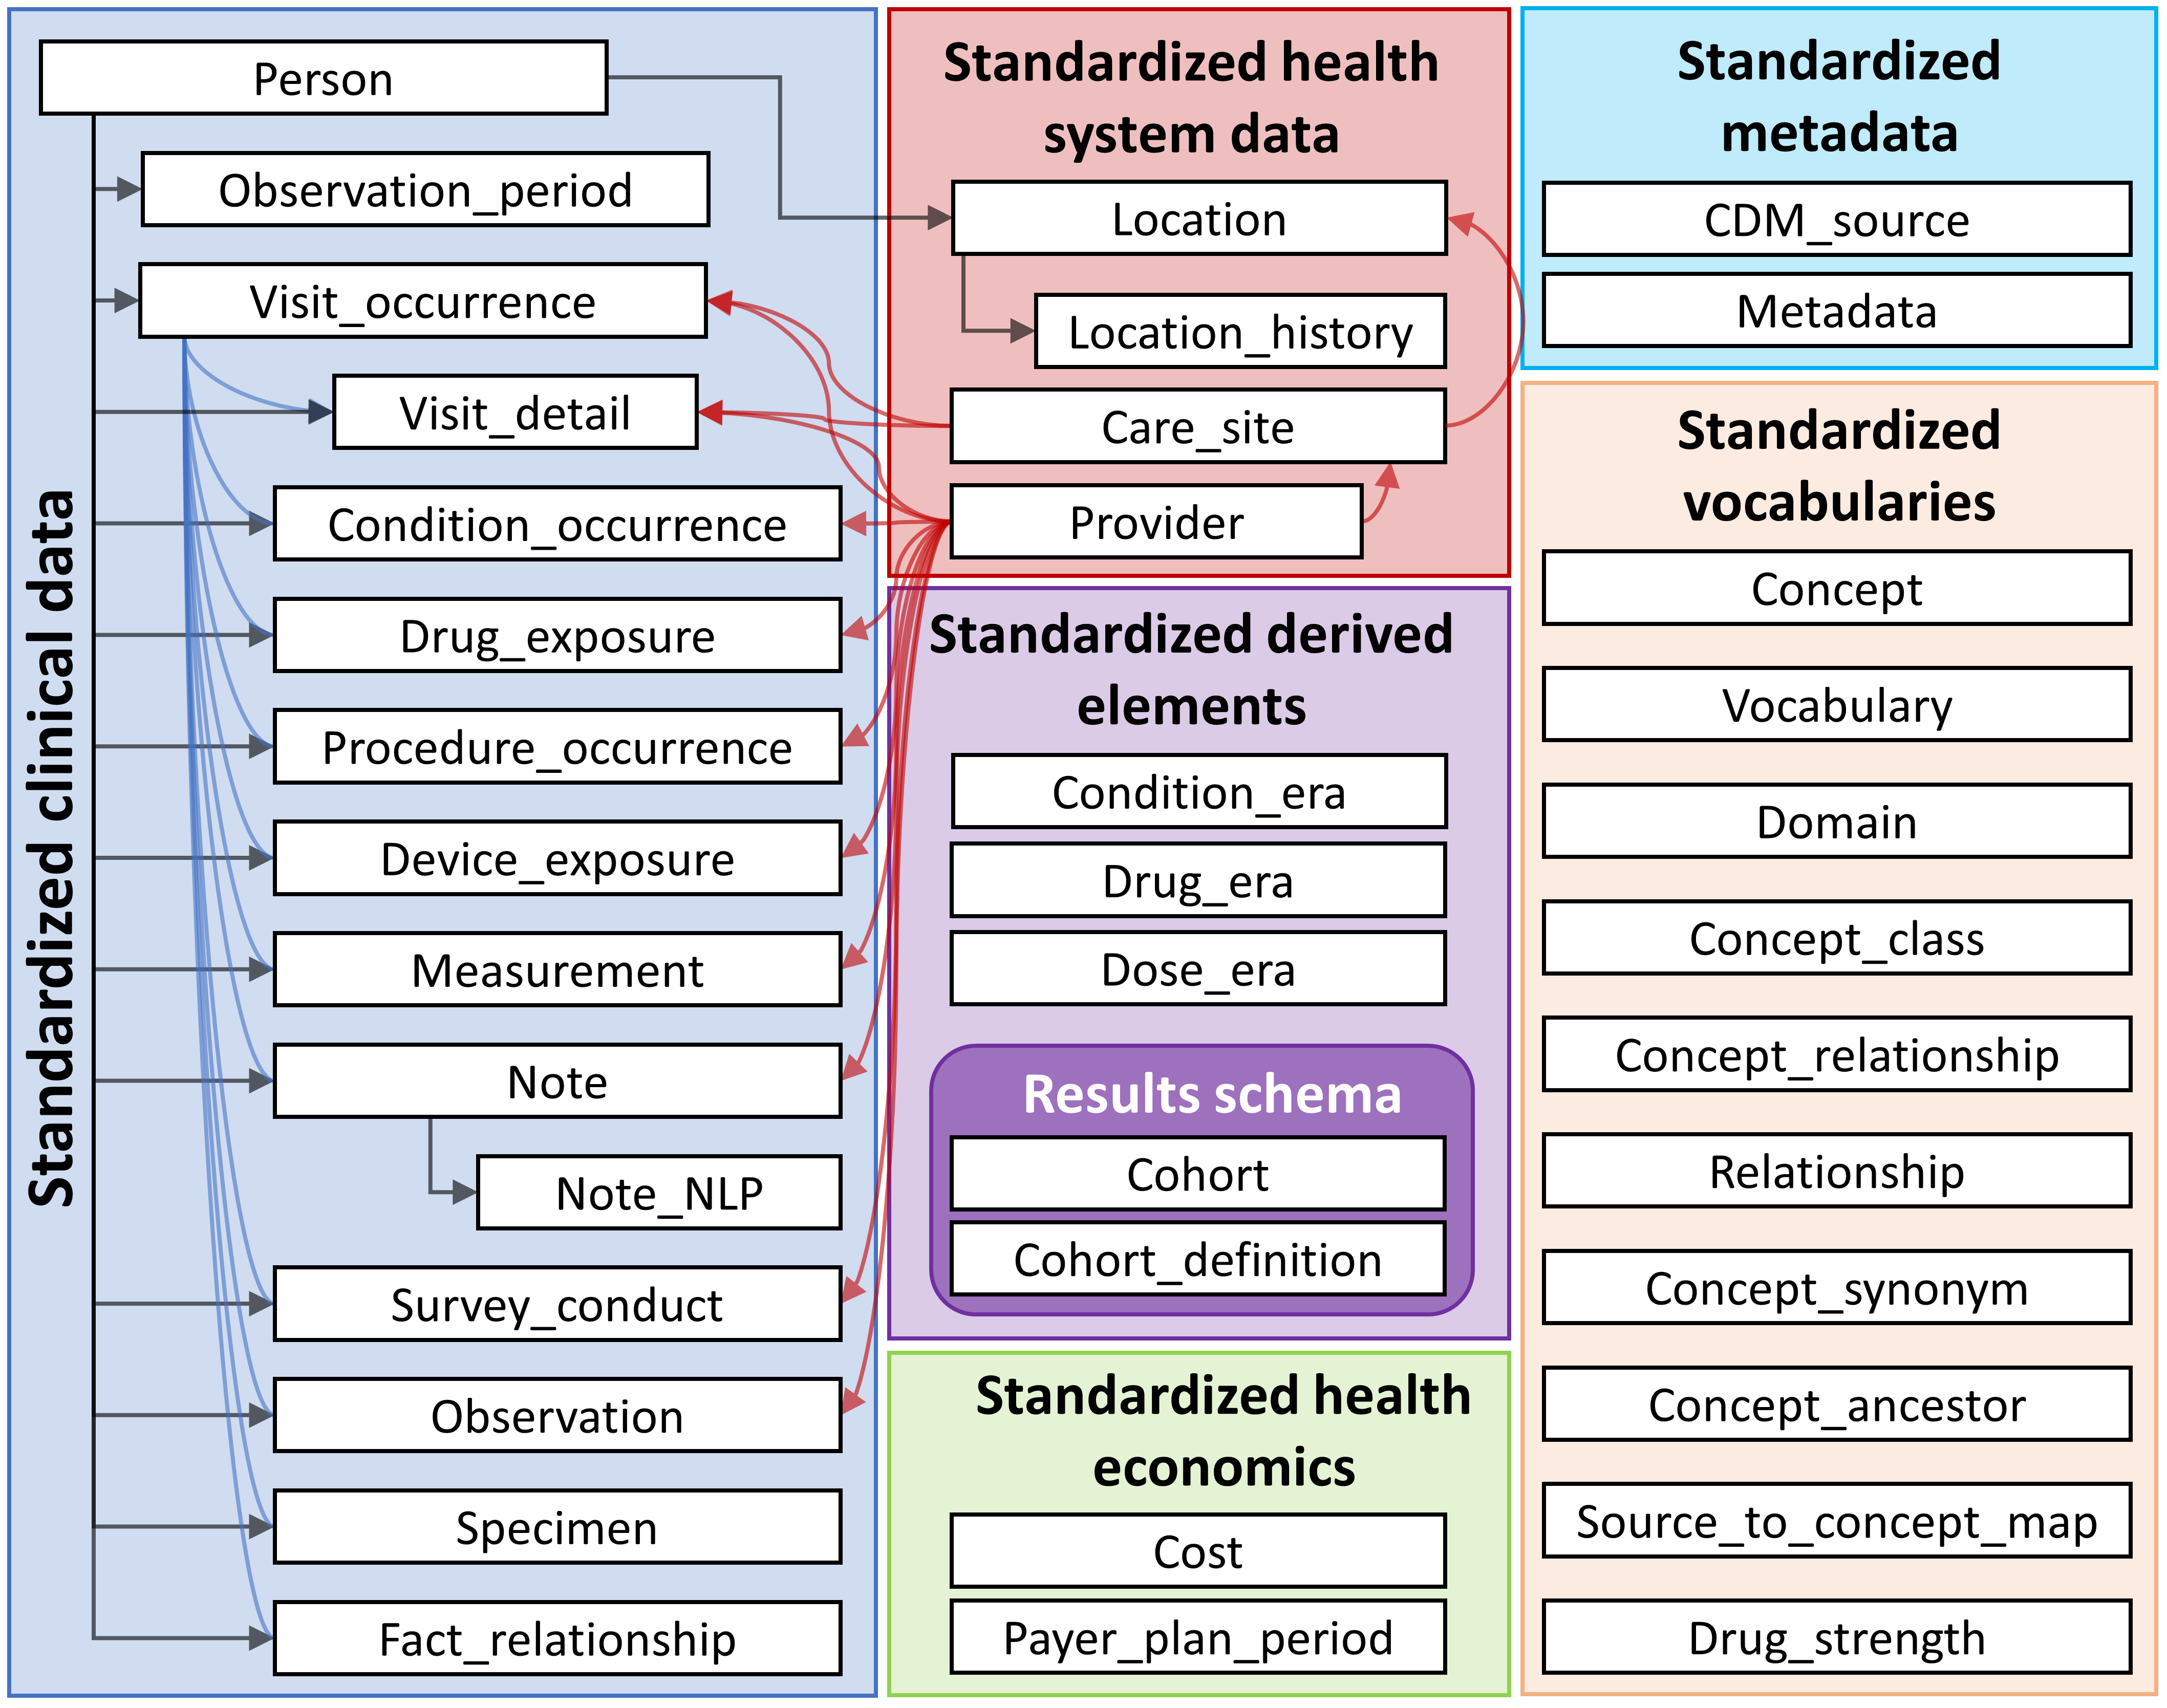
\includegraphics[width=1\linewidth]{images/CommonDataModel/cdmDiagram} \caption{Overview of all tables in the CDM version 6.0. Note that not all relationships between tables are shown.}\label{fig:cdmDiagram}
\end{figure}

\section{Design Principles}\label{design-principles}

The CDM is designed to include all observational health data elements
(experiences of the patient receiving health care) that are relevant for
analysis use cases to support the generation of reliable scientific
evidence about disease natural history, healthcare delivery, effects of
medical interventions, the identification of demographic information,
health care interventions and outcomes.

Therefore, the CDM is designed to store observational data to allow for
research, under the following principles:

\begin{itemize}
\tightlist
\item
  \textbf{Suitability for purpose}: The CDM aims to provide data
  organized in a way optimal for analysis, rather than for the purpose
  of addressing the operational needs of health care providers or
  payers.
\item
  \textbf{Data protection}: All data that might jeopardize the identity
  and protection of patients, such as names, precise birthdays etc. are
  limited. Exceptions are possible where the research expressly requires
  more detailed information, such as precise birth dates for the study
  of infants.
\item
  \textbf{Design of domains}: The domains are modeled in a
  person-centric relational data model, where for each record the
  identity of the person and a date is captured as a minimum.
\item
  \textbf{Rationale for domains}: Domains are identified and separately
  defined in an entity-relationship model if they have an analysis use
  case and the domain has specific attributes that are not otherwise
  applicable. All other data can be preserved as an observation in an
  entity-attribute-value structure.
\item
  \textbf{Standardized Vocabularies}: To standardize the content of
  those records, the CDM relies on the Standardized Vocabularies
  containing all necessary and appropriate corresponding standard
  healthcare concepts.
\item
  \textbf{Reuse of existing vocabularies}: If possible, these concepts
  are leveraged from national or industry standardization or vocabulary
  definition organizations or initiatives, such as the National Library
  of Medicine, the Department of Veterans' Affairs, the Center of
  Disease Control and Prevention, etc.
\item
  \textbf{Maintaining source codes}: Even though all codes are mapped to
  the Standardized Vocabularies, the model also stores the original
  source code to ensure no information is lost.
\item
  \textbf{Technology neutrality}: The CDM does not require a specific
  technology. It can be realized in any relational database, such as
  Oracle, SQL Server etc., or as SAS analytical datasets.
\item
  \textbf{Scalability}: The CDM is optimized for data processing and
  computational analysis to accommodate data sources that vary in size,
  including databases with up to hundreds of millions of persons and
  billions of clinical observations.
\item
  \textbf{Backwards compatibility}: All changes from previous CDMs are
  clearly delineated in the github repository
  \href{https://github.com/OHDSI/CommonDataModel}{(https://github.com/OHDSI/CommonDataModel)}.
  Older versions of the CDM can be easily created from the CDMv5, and no
  information is lost that was present previously.
\end{itemize}

\section{Data Model Conventions}\label{data-model-conventions}

There are a number of implicit and explicit conventions that have been
adopted in the CDM. Developers of methods that run against the CDM need
to understand these conventions.

\subsection{General conventions of the model}\label{model-conv}

The OMOP CDM is considered a ``person-centric'' model, meaning that the
people (or patients) drive the event and observation tables. At a
minimum, the tables have a foreign key into the PERSON table and a date.
This allows for a longitudinal view on all healthcare-relevant events by
person. The exceptions from this rule are the standardized health system
data tables, which are linked directly to events of the various domains.

\subsection{General conventions of
schemas}\label{general-conventions-of-schemas}

New to CDM v6.0 is the concept of schemas. This allows for more
separation between read-only and writeable tables. The clinical data,
event, and vocabulary tables are in the ``CDM'' schema and are
considered read-only to the end user. This means that the tables can be
queried but no information can be accidentally removed or written over
except by the database administrator. Tables that need to be manipulated
by web-based tools or end users have moved to the ``Results'' schema.
Currently the only two tables in the ``Results'' schema are COHORT and
COHORT\_DEFINITON, \textbf{Todo: add a sentence explaining that these
tables describe groups of interest that the user might define, put in
links to the later sections} though likely more will be added over the
course of v6.0 point releases. These tables can be written to, meaning
that a cohort created in ATLAS or by a user can be stored in the COHORT
table and accessed at a later date. This does mean that cohorts in the
COHORT table can be manipulated by anyone so it is always recommended
that the SQL code used to create the cohort be saved along with the
project or analysis in the event it needs to be regenerated.

\subsection{General conventions of data
tables}\label{general-conventions-of-data-tables}

The CDM is platform-independent. Data types are defined generically
using ANSI SQL data types (VARCHAR, INTEGER, FLOAT, DATE, DATETIME,
CLOB). Precision is provided only for VARCHAR. It reflects the minimal
required string length and can be expanded within a CDM instantiation.
The CDM does not prescribe the date and datetime format. Standard
queries against CDM may vary for local instantiations and date/datetime
configurations.

In most cases, the first field in each table ends in ``\_id``,
containing a record identifier that can be used as a foreign key in
another table. For example, the CONDITION\_OCCURRENCE table contains the
field visit\_occurrence\_id which is a foreign key to the
VISIT\_OCCURRENCE table where visit\_occurrence\_id is the primary key.

\subsection{General conventions of
fields}\label{general-conventions-of-fields}

Variable names across all tables follow one convention:

\begin{longtable}[]{@{}ll@{}}
\caption{\label{tab:fieldConventions} Field name
conventions.}\tabularnewline
\toprule
\begin{minipage}[b]{0.34\columnwidth}\raggedright\strut
Notation\strut
\end{minipage} & \begin{minipage}[b]{0.61\columnwidth}\raggedright\strut
Description\strut
\end{minipage}\tabularnewline
\midrule
\endfirsthead
\toprule
\begin{minipage}[b]{0.34\columnwidth}\raggedright\strut
Notation\strut
\end{minipage} & \begin{minipage}[b]{0.61\columnwidth}\raggedright\strut
Description\strut
\end{minipage}\tabularnewline
\midrule
\endhead
\begin{minipage}[t]{0.34\columnwidth}\raggedright\strut
{[}entity{]}\_id\strut
\end{minipage} & \begin{minipage}[t]{0.61\columnwidth}\raggedright\strut
Unique identifiers for key entities, which can serve as foreign keys to
establish relationships across entities. For example, person\_id
uniquely identifies each individual. visit\_occurrence\_id uniquely
identifies a PERSON encounter at a point of care.\strut
\end{minipage}\tabularnewline
\begin{minipage}[t]{0.34\columnwidth}\raggedright\strut
{[}entity{]}\_source\_value\strut
\end{minipage} & \begin{minipage}[t]{0.61\columnwidth}\raggedright\strut
Verbatim information from the source data, typically used in ETL to map
to concept\_id, and not to be used by any standard analytics. For
example, condition\_source\_value = `787.02' was the ICD-9 code captured
as a diagnosis from the administrative claim.\strut
\end{minipage}\tabularnewline
\begin{minipage}[t]{0.34\columnwidth}\raggedright\strut
{[}entity{]}\_concept\_id\strut
\end{minipage} & \begin{minipage}[t]{0.61\columnwidth}\raggedright\strut
Foreign key into the Standardized Vocabularies (i.e.~the standard
concept attribute for the corresponding term is true), which serves as
the primary basis for all standardized analytics. For example,
condition\_concept\_id =
\href{http://athena.ohdsi.org/search-terms/terms/31967}{31967} contains
the reference value for the SNOMED concept of ``Nausea''.\strut
\end{minipage}\tabularnewline
\begin{minipage}[t]{0.34\columnwidth}\raggedright\strut
{[}entity{]}\_source\_concept\_id\strut
\end{minipage} & \begin{minipage}[t]{0.61\columnwidth}\raggedright\strut
Foreign key into the Standardized Vocabularies representing the concept
and terminology used in the source data, when applicable. For example,
condition\_source\_concept\_id =
\href{http://athena.ohdsi.org/search-terms/terms/45431665}{45431665}
denotes the concept of ``Nausea'' in the Read terminology; the analogous
condition\_concept\_id is
\href{http://athena.ohdsi.org/search-terms/terms/31967}{31967}, since
SNOMED-CT is the Standardized Vocabulary for most clinical diagnoses and
findings.\strut
\end{minipage}\tabularnewline
\begin{minipage}[t]{0.34\columnwidth}\raggedright\strut
{[}entity{]}\_type\_concept\_id\strut
\end{minipage} & \begin{minipage}[t]{0.61\columnwidth}\raggedright\strut
Delineates the origin of the source information, standardized within the
Standardized Vocabularies. For example, drug\_type\_concept\_id can
allow analysts to discriminate between ``Pharmacy dispensing'' and
``Prescription written''\strut
\end{minipage}\tabularnewline
\bottomrule
\end{longtable}

\subsection{Representation of content through
Concepts}\label{representation-of-content-through-concepts}

In CDM data tables the content of each record is represented using
Concepts. Concepts are stored in event tables with their concept IDs as
foreign keys to the CONCEPT table, which contains concepts necessary to
describe the healthcare experience of a patient. If a Standard Concept
does not exist or cannot be identified, the concept ID 0 is used,
representing a non-existing concept or un-mappable source value.

Records in the CONCEPT table contain detailed information about each
concept (name, domain, class etc.). Concepts, Concept Relationships,
Concept Ancestors and other information relating to Concepts is
contained in the tables of the Standardized Vocabularies.

\subsection{Difference between Concept IDs and Source
Values}\label{difference-between-concept-ids-and-source-values}

Many tables contain equivalent information in multiple places: As a
Source Value, a Source Concept and as a Standard Concept.

\begin{itemize}
\tightlist
\item
  \textbf{Source Values} contain the codes from public code systems such
  as ICD-9-CM, NDC, CPT-4, READ etc. or locally controlled vocabularies
  (such as F for female and M for male) copied from the source data.
  Source Values are stored in the {[}entity{]}\_source\_value fields in
  the data tables.
\item
  \textbf{Concepts} are CDM-specific entities that represent the meaning
  of a clinical fact. Most concepts are based on code systems used in
  healthcare (called Source Concepts), while others were created de-novo
  (concept\_code = ``OMOP generated''). Concepts have unique IDs across
  all domains.
\item
  \textbf{Source Concepts} are the concepts that represent the code used
  in the source. Source Concepts are only used for common healthcare
  code systems, not for OMOP-generated Concepts. Source Concepts are
  stored in the {[}entity{]}\_source\_concept\_id field in the data
  tables.
\item
  \textbf{Standard Concepts} are those concepts that are used to define
  the unique meaning of a clinical entity. For each entity there is one
  Standard Concept. Standard Concepts are typically drawn from existing
  public vocabulary sources. Concepts that have the equivalent meaning
  to a Standard Concept are mapped to the Standard Concept. Standard
  Concepts are referred to in the {[}entity{]}\_concept\_id field of the
  data tables.
\end{itemize}

Source Values are only provided for convenience and quality assurance
(QA) purposes. Source Values and Source Concepts are optional, while
\textbf{Standard Concepts are mandatory}. Source Values may contain
information that is only meaningful in the context of a specific data
source. This mandatory use of Standard Concepts is what allows all OHDSI
collaborators to speak the same language. For example, let's look at the
condition ``Pulmonary Tuberculosis'' (TB). Figure \ref{fig:pulmTubICD9}
shows that the ICD9CM code for TB is 011.

\begin{figure}

{\centering 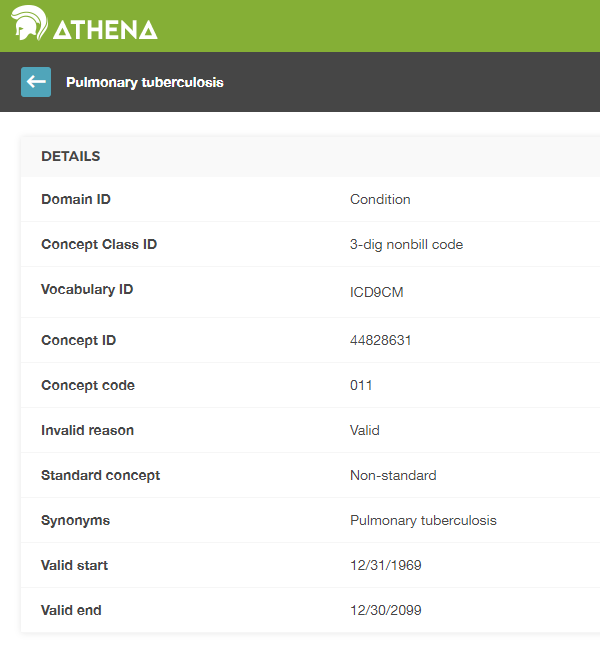
\includegraphics[width=0.75\linewidth]{images/CommonDataModel/pulmTubICD9} 

}

\caption{ICD9CM code for Pulmonary Tuberculosis}\label{fig:pulmTubICD9}
\end{figure}

Without the use of a standard way to represent TB the code 011 could be
interpreted as ``Hospital Inpatient (Including Medicare Part A)'' in the
UB04 vocabulary, or as ``Nervous System Neoplasms without Complications,
Comorbidities'' in the DRG vocabulary. This is where Concept IDs, both
Source and Standard, are valuable. The Concept ID that represents the
011 ICD9CM code is
\href{http://athena.ohdsi.org/search-terms/terms/44828631}{44828631}.
This differentiates the ICD9CM from the UBO4 and from the DRG. The
Standard Concept that ICD9CM code maps to is
\href{http://athena.ohdsi.org/search-terms/terms/253954}{253954} as
shown in figure \ref{fig:pulmTubMap} by the relationship ``Non-standard
to Standard map (OMOP)''. This same mapping relationship exists between
Read, ICD10, CIEL, and MeSH codes, among others, so that any research
that references the standard SNOMED concept is sure to include all
supported source codes.

\begin{figure}
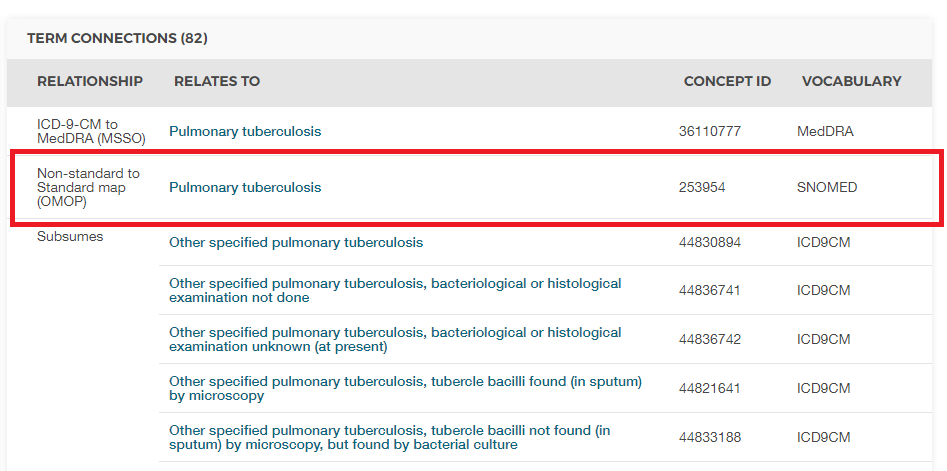
\includegraphics[width=1\linewidth]{images/CommonDataModel/pulmTubMap} \caption{SNOMED code for Pulmonary Tuberculosis}\label{fig:pulmTubMap}
\end{figure}

An example of how this relationship is depicted in the tables is shown
in Table \ref{tab:conditionOccurrence}.

\section{OMOP CDM Standardized
Tables}\label{omop-cdm-standardized-tables}

The OMOP CDM contains 16 Clinical data tables, 10 Vocabulary tables, 2
Metadata tables, 4 Health System data tables, 2 Health Economics data
tables, 3 standardized derived elements, and 2 results schema tables.
These tables are fully specified in the CDM Wiki\footnote{\url{https://github.com/OHDSI/CommonDataModel/wiki}{]}(\url{https://github.com/OHDSI/CommonDataModel/wiki}}.

To illustrate how these tables are used in practice the data of one
person will be used as a common thread throughout the rest of the
chapter. While part of the CDM the Vocabulary tables are not covered
here, rather, they are detailed in depth in Chapter
\ref{StandardizedVocabularies}.

\subsection{Running Example:
Endometriosis}\label{running-example-endometriosis}

Endometriosis is a painful condition whereby cells normally found in the
lining of a woman's uterus occur elsewhere in the body. Severe cases can
lead to infertility, bowel, and bladder problems. The following sections
will detail one patient's experience with this disease and how her
clinical experience might be represented in the Common Data Model.

\begin{center}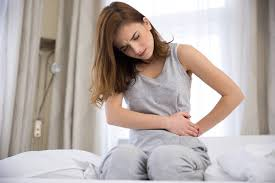
\includegraphics[width=0.5\linewidth]{images/CommonDataModel/Lauren} \end{center}

\begin{quote}
Every step of this painfull journey I had to convince everyone how much
pain I was in.
\end{quote}

Lauren had been experiencing endometriosis symptoms for many year;
however, it took a ruptured cyst in her ovary before she was diagnosed.
You can read more about Lauren at
\url{https://www.endometriosis-uk.org/laurens-story}.

\subsection{PERSON table}\label{person}

As the Common Data Model is a person-centric model (see section
\ref{model-conv}) let's start with how she would be represented in the
PERSON table.

\textbf{What do we know about Lauren?}

\begin{itemize}
\tightlist
\item
  She is a 36-year-old woman
\item
  Her birthday is 12-March-1982
\item
  She is white
\item
  She is english
\end{itemize}

With that in mind, her PERSON table might look something like this:

\begin{longtable}[]{@{}lll@{}}
\caption{\label{tab:person} The PERSON table.}\tabularnewline
\toprule
\begin{minipage}[b]{0.28\columnwidth}\raggedright\strut
Column name\strut
\end{minipage} & \begin{minipage}[b]{0.16\columnwidth}\raggedright\strut
Value\strut
\end{minipage} & \begin{minipage}[b]{0.48\columnwidth}\raggedright\strut
Explanation\strut
\end{minipage}\tabularnewline
\midrule
\endfirsthead
\toprule
\begin{minipage}[b]{0.28\columnwidth}\raggedright\strut
Column name\strut
\end{minipage} & \begin{minipage}[b]{0.16\columnwidth}\raggedright\strut
Value\strut
\end{minipage} & \begin{minipage}[b]{0.48\columnwidth}\raggedright\strut
Explanation\strut
\end{minipage}\tabularnewline
\midrule
\endhead
\begin{minipage}[t]{0.28\columnwidth}\raggedright\strut
person\_id\strut
\end{minipage} & \begin{minipage}[t]{0.16\columnwidth}\raggedright\strut
1\strut
\end{minipage} & \begin{minipage}[t]{0.48\columnwidth}\raggedright\strut
person\_id should be an integer, either directly from the source or
generated as part of the build process.\strut
\end{minipage}\tabularnewline
\begin{minipage}[t]{0.28\columnwidth}\raggedright\strut
gender\_concept\_id\strut
\end{minipage} & \begin{minipage}[t]{0.16\columnwidth}\raggedright\strut
8532\strut
\end{minipage} & \begin{minipage}[t]{0.48\columnwidth}\raggedright\strut
The concept ID referring to female gender is
\href{http://athena.ohdsi.org/search-terms/terms/8532}{8532}.\strut
\end{minipage}\tabularnewline
\begin{minipage}[t]{0.28\columnwidth}\raggedright\strut
year\_of\_birth\strut
\end{minipage} & \begin{minipage}[t]{0.16\columnwidth}\raggedright\strut
1982\strut
\end{minipage} & \begin{minipage}[t]{0.48\columnwidth}\raggedright\strut
\strut
\end{minipage}\tabularnewline
\begin{minipage}[t]{0.28\columnwidth}\raggedright\strut
month\_of\_birth\strut
\end{minipage} & \begin{minipage}[t]{0.16\columnwidth}\raggedright\strut
3\strut
\end{minipage} & \begin{minipage}[t]{0.48\columnwidth}\raggedright\strut
\strut
\end{minipage}\tabularnewline
\begin{minipage}[t]{0.28\columnwidth}\raggedright\strut
day\_of\_birth\strut
\end{minipage} & \begin{minipage}[t]{0.16\columnwidth}\raggedright\strut
12\strut
\end{minipage} & \begin{minipage}[t]{0.48\columnwidth}\raggedright\strut
\strut
\end{minipage}\tabularnewline
\begin{minipage}[t]{0.28\columnwidth}\raggedright\strut
birth\_datetime\strut
\end{minipage} & \begin{minipage}[t]{0.16\columnwidth}\raggedright\strut
1982-03-12 00:00:00\strut
\end{minipage} & \begin{minipage}[t]{0.48\columnwidth}\raggedright\strut
When the time is not known midnight is used.\strut
\end{minipage}\tabularnewline
\begin{minipage}[t]{0.28\columnwidth}\raggedright\strut
death\_datetime\strut
\end{minipage} & \begin{minipage}[t]{0.16\columnwidth}\raggedright\strut
\strut
\end{minipage} & \begin{minipage}[t]{0.48\columnwidth}\raggedright\strut
\strut
\end{minipage}\tabularnewline
\begin{minipage}[t]{0.28\columnwidth}\raggedright\strut
race\_concept\_id\strut
\end{minipage} & \begin{minipage}[t]{0.16\columnwidth}\raggedright\strut
8527\strut
\end{minipage} & \begin{minipage}[t]{0.48\columnwidth}\raggedright\strut
The concept ID referring to white race is
\href{http://athena.ohdsi.org/search-terms/terms/8527}{8527}.\strut
\end{minipage}\tabularnewline
\begin{minipage}[t]{0.28\columnwidth}\raggedright\strut
ethnicity\_concept\_ id\strut
\end{minipage} & \begin{minipage}[t]{0.16\columnwidth}\raggedright\strut
38003564\strut
\end{minipage} & \begin{minipage}[t]{0.48\columnwidth}\raggedright\strut
Typically hispanic status is stored for ethnicity. The concept ID
\href{http://athena.ohdsi.org/search-terms/terms/38003564}{38003564}
refers to ``Not hispanic''.\strut
\end{minipage}\tabularnewline
\begin{minipage}[t]{0.28\columnwidth}\raggedright\strut
location\_id\strut
\end{minipage} & \begin{minipage}[t]{0.16\columnwidth}\raggedright\strut
\strut
\end{minipage} & \begin{minipage}[t]{0.48\columnwidth}\raggedright\strut
Her address is not known.\strut
\end{minipage}\tabularnewline
\begin{minipage}[t]{0.28\columnwidth}\raggedright\strut
provider\_id\strut
\end{minipage} & \begin{minipage}[t]{0.16\columnwidth}\raggedright\strut
\strut
\end{minipage} & \begin{minipage}[t]{0.48\columnwidth}\raggedright\strut
Her primary care provider is not known.\strut
\end{minipage}\tabularnewline
\begin{minipage}[t]{0.28\columnwidth}\raggedright\strut
care\_site\_id\strut
\end{minipage} & \begin{minipage}[t]{0.16\columnwidth}\raggedright\strut
\strut
\end{minipage} & \begin{minipage}[t]{0.48\columnwidth}\raggedright\strut
Her primary care site is not known.\strut
\end{minipage}\tabularnewline
\begin{minipage}[t]{0.28\columnwidth}\raggedright\strut
person\_source\_value\strut
\end{minipage} & \begin{minipage}[t]{0.16\columnwidth}\raggedright\strut
1\strut
\end{minipage} & \begin{minipage}[t]{0.48\columnwidth}\raggedright\strut
Typically this would be her identifier in the source data, though often
is it the same as the person\_id.\strut
\end{minipage}\tabularnewline
\begin{minipage}[t]{0.28\columnwidth}\raggedright\strut
gender\_source\_value\strut
\end{minipage} & \begin{minipage}[t]{0.16\columnwidth}\raggedright\strut
F\strut
\end{minipage} & \begin{minipage}[t]{0.48\columnwidth}\raggedright\strut
The gender value as it appears in the source is stored here.\strut
\end{minipage}\tabularnewline
\begin{minipage}[t]{0.28\columnwidth}\raggedright\strut
gender\_source\_ concept\_id\strut
\end{minipage} & \begin{minipage}[t]{0.16\columnwidth}\raggedright\strut
0\strut
\end{minipage} & \begin{minipage}[t]{0.48\columnwidth}\raggedright\strut
If the gender value in the source was coded using a vocabulary
recognized by OHDSI, that concept ID would go here. For example, if her
gender was ``Sex-F'' in the source and it was stated to be in the
PCORNet vocabulary concept ID
\href{http://athena.ohdsi.org/search-terms/terms/44814665}{44814665}
would go in this field.\strut
\end{minipage}\tabularnewline
\begin{minipage}[t]{0.28\columnwidth}\raggedright\strut
race\_source\_value\strut
\end{minipage} & \begin{minipage}[t]{0.16\columnwidth}\raggedright\strut
white\strut
\end{minipage} & \begin{minipage}[t]{0.48\columnwidth}\raggedright\strut
The race value as it appears in the source is stored here.\strut
\end{minipage}\tabularnewline
\begin{minipage}[t]{0.28\columnwidth}\raggedright\strut
race\_source\_concept\_ id\strut
\end{minipage} & \begin{minipage}[t]{0.16\columnwidth}\raggedright\strut
0\strut
\end{minipage} & \begin{minipage}[t]{0.48\columnwidth}\raggedright\strut
Same principle as gender\_source\_concept\_id.\strut
\end{minipage}\tabularnewline
\begin{minipage}[t]{0.28\columnwidth}\raggedright\strut
ethnicity\_source\_ value\strut
\end{minipage} & \begin{minipage}[t]{0.16\columnwidth}\raggedright\strut
english\strut
\end{minipage} & \begin{minipage}[t]{0.48\columnwidth}\raggedright\strut
The ethnicity value as it appears in the source is stored here.\strut
\end{minipage}\tabularnewline
\begin{minipage}[t]{0.28\columnwidth}\raggedright\strut
ethnicity\_source\_ concept\_id\strut
\end{minipage} & \begin{minipage}[t]{0.16\columnwidth}\raggedright\strut
0\strut
\end{minipage} & \begin{minipage}[t]{0.48\columnwidth}\raggedright\strut
Same principle as gender\_source\_concept\_id.\strut
\end{minipage}\tabularnewline
\bottomrule
\end{longtable}

\subsection{OBSERVATION\_PERIOD table}\label{observationPeriod}

The OBSERVATION\_PERIOD table is designed to define the amount of time
for which a patient's clinical events are recorded in the source system.
For US healthcare insurance claims this is typically the enrollment
period of the patient. When working with data from electronic health
records (EHR) often the first record in the system is considered the
observation\_period\_start\_date and the latest record is considered the
observation\_period\_end\_date with the understanding that only the
clinical events that happened within that particular system were
recorded.

\textbf{How can we determine Lauren's observation period?}

Lauren's information as shown in Table \ref{tab:encounters} is most
similar to EHR data in that we only have records of her encounters from
which to determine her observation period.

\begin{longtable}[]{@{}llll@{}}
\caption{\label{tab:encounters} Lauren's healthcare
encounters.}\tabularnewline
\toprule
Encounter ID & Start date & Stop date & Type\tabularnewline
\midrule
\endfirsthead
\toprule
Encounter ID & Start date & Stop date & Type\tabularnewline
\midrule
\endhead
70 & 2010-01-06 & 2010-01-06 & outpatient\tabularnewline
80 & 2011-01-06 & 2011-01-06 & outpatient\tabularnewline
90 & 2012-01-06 & 2012-01-06 & outpatient\tabularnewline
100 & 2013-01-07 & 2013-01-07 & outpatient\tabularnewline
101 & 2013-01-14 & 2013-01-14 & ambulatory\tabularnewline
102 & 2013-01-17 & 2013-01-24 & inpatient\tabularnewline
\bottomrule
\end{longtable}

Based on the encounter records her OBSERVATION\_PERIOD table might look
something like this:

\begin{longtable}[]{@{}lll@{}}
\caption{\label{tab:observationPeriod} The OBSERVATION\_PERIOD
table.}\tabularnewline
\toprule
\begin{minipage}[b]{0.28\columnwidth}\raggedright\strut
Column name\strut
\end{minipage} & \begin{minipage}[b]{0.16\columnwidth}\raggedright\strut
Value\strut
\end{minipage} & \begin{minipage}[b]{0.48\columnwidth}\raggedright\strut
Explanation\strut
\end{minipage}\tabularnewline
\midrule
\endfirsthead
\toprule
\begin{minipage}[b]{0.28\columnwidth}\raggedright\strut
Column name\strut
\end{minipage} & \begin{minipage}[b]{0.16\columnwidth}\raggedright\strut
Value\strut
\end{minipage} & \begin{minipage}[b]{0.48\columnwidth}\raggedright\strut
Explanation\strut
\end{minipage}\tabularnewline
\midrule
\endhead
\begin{minipage}[t]{0.28\columnwidth}\raggedright\strut
observation\_period\_ id\strut
\end{minipage} & \begin{minipage}[t]{0.16\columnwidth}\raggedright\strut
1\strut
\end{minipage} & \begin{minipage}[t]{0.48\columnwidth}\raggedright\strut
This is typically an autogenerated field that creates a unique ID number
for each record in the table.\strut
\end{minipage}\tabularnewline
\begin{minipage}[t]{0.28\columnwidth}\raggedright\strut
person\_id\strut
\end{minipage} & \begin{minipage}[t]{0.16\columnwidth}\raggedright\strut
1\strut
\end{minipage} & \begin{minipage}[t]{0.48\columnwidth}\raggedright\strut
This comes from the PERSON table and links PERSON and
OBSERVATION\_PERIOD.\strut
\end{minipage}\tabularnewline
\begin{minipage}[t]{0.28\columnwidth}\raggedright\strut
observation\_period\_ start\_date\strut
\end{minipage} & \begin{minipage}[t]{0.16\columnwidth}\raggedright\strut
2010-01-06\strut
\end{minipage} & \begin{minipage}[t]{0.48\columnwidth}\raggedright\strut
This is the start date of her earliest encounter on record.\strut
\end{minipage}\tabularnewline
\begin{minipage}[t]{0.28\columnwidth}\raggedright\strut
observation\_period\_ end\_date\strut
\end{minipage} & \begin{minipage}[t]{0.16\columnwidth}\raggedright\strut
2013-01-24\strut
\end{minipage} & \begin{minipage}[t]{0.48\columnwidth}\raggedright\strut
This is the end date of her latest encounter on record.\strut
\end{minipage}\tabularnewline
\begin{minipage}[t]{0.28\columnwidth}\raggedright\strut
period\_type\_ concept\_id\strut
\end{minipage} & \begin{minipage}[t]{0.16\columnwidth}\raggedright\strut
44814725\strut
\end{minipage} & \begin{minipage}[t]{0.48\columnwidth}\raggedright\strut
The best option in the Vocabulary with the concept class ``Obs Period
Type'' is
\href{http://athena.ohdsi.org/search-terms/terms/44814724}{44814724},
which stands for ``Period covering healthcare encounters''.\strut
\end{minipage}\tabularnewline
\bottomrule
\end{longtable}

\subsection{VISIT\_OCCURRENCE}\label{visitOccurrence}

The VISIT\_OCCURRENCE table houses information about a patient's
encounters with the health care system. Within the OHDSI vernacular
these are referred to as visits and are considered to be discreet
events. There are 12 categories of visits though the most common are
inpatient, outpatient, emergency and long term care.

\textbf{How do we represent Lauren's encounters as visits?}

As an example let's represent the inpatient encounter in Table
\ref{tab:encounters} as a record in the VISIT\_OCCURRENCE table.

\begin{longtable}[]{@{}lll@{}}
\caption{\label{tab:visitOccurrence} The VISIT\_OCCURRENCE
table.}\tabularnewline
\toprule
\begin{minipage}[b]{0.28\columnwidth}\raggedright\strut
Column name\strut
\end{minipage} & \begin{minipage}[b]{0.16\columnwidth}\raggedright\strut
Value\strut
\end{minipage} & \begin{minipage}[b]{0.48\columnwidth}\raggedright\strut
Explanation\strut
\end{minipage}\tabularnewline
\midrule
\endfirsthead
\toprule
\begin{minipage}[b]{0.28\columnwidth}\raggedright\strut
Column name\strut
\end{minipage} & \begin{minipage}[b]{0.16\columnwidth}\raggedright\strut
Value\strut
\end{minipage} & \begin{minipage}[b]{0.48\columnwidth}\raggedright\strut
Explanation\strut
\end{minipage}\tabularnewline
\midrule
\endhead
\begin{minipage}[t]{0.28\columnwidth}\raggedright\strut
visit\_occurrence\_id\strut
\end{minipage} & \begin{minipage}[t]{0.16\columnwidth}\raggedright\strut
514\strut
\end{minipage} & \begin{minipage}[t]{0.48\columnwidth}\raggedright\strut
This is typically an autogenerated field that creates a unique ID number
for each visit on the person's record in the converted CDM
database.\strut
\end{minipage}\tabularnewline
\begin{minipage}[t]{0.28\columnwidth}\raggedright\strut
person\_id\strut
\end{minipage} & \begin{minipage}[t]{0.16\columnwidth}\raggedright\strut
1\strut
\end{minipage} & \begin{minipage}[t]{0.48\columnwidth}\raggedright\strut
This comes from the PERSON table and links PERSON and
VISIT\_OCCURRENCE.\strut
\end{minipage}\tabularnewline
\begin{minipage}[t]{0.28\columnwidth}\raggedright\strut
visit\_concept\_id\strut
\end{minipage} & \begin{minipage}[t]{0.16\columnwidth}\raggedright\strut
9201\strut
\end{minipage} & \begin{minipage}[t]{0.48\columnwidth}\raggedright\strut
The concept ID referring to an inpatient visit is
\href{http://athena.ohdsi.org/search-terms/terms/9201}{9201}.\strut
\end{minipage}\tabularnewline
\begin{minipage}[t]{0.28\columnwidth}\raggedright\strut
visit\_start\_date\strut
\end{minipage} & \begin{minipage}[t]{0.16\columnwidth}\raggedright\strut
2013-01-17\strut
\end{minipage} & \begin{minipage}[t]{0.48\columnwidth}\raggedright\strut
The start date of the visit.\strut
\end{minipage}\tabularnewline
\begin{minipage}[t]{0.28\columnwidth}\raggedright\strut
visit\_start\_datetime\strut
\end{minipage} & \begin{minipage}[t]{0.16\columnwidth}\raggedright\strut
2013-01-17 00:00:00\strut
\end{minipage} & \begin{minipage}[t]{0.48\columnwidth}\raggedright\strut
The date and time of the visit started. When time is unknown midnight is
used.\strut
\end{minipage}\tabularnewline
\begin{minipage}[t]{0.28\columnwidth}\raggedright\strut
visit\_end\_date\strut
\end{minipage} & \begin{minipage}[t]{0.16\columnwidth}\raggedright\strut
2013-01-24\strut
\end{minipage} & \begin{minipage}[t]{0.48\columnwidth}\raggedright\strut
The end date of the visit. If this is a one-day visit the end date
should match the start date.\strut
\end{minipage}\tabularnewline
\begin{minipage}[t]{0.28\columnwidth}\raggedright\strut
visit\_end\_datetime\strut
\end{minipage} & \begin{minipage}[t]{0.16\columnwidth}\raggedright\strut
2013-01-24 00:00:00\strut
\end{minipage} & \begin{minipage}[t]{0.48\columnwidth}\raggedright\strut
The date and time of the visit end. If time is unknown midnight is
used.\strut
\end{minipage}\tabularnewline
\begin{minipage}[t]{0.28\columnwidth}\raggedright\strut
visit\_type\_concept\_ id\strut
\end{minipage} & \begin{minipage}[t]{0.16\columnwidth}\raggedright\strut
32034\strut
\end{minipage} & \begin{minipage}[t]{0.48\columnwidth}\raggedright\strut
This column is intended to provide information about the provenance of
the visit record, i.e.~does it come from an insurance claim, hospital
billing record, EHR record, etc. For this example the concept ID
\href{http://athena.ohdsi.org/search-terms/terms/32035}{32035} (``Visit
derived from EHR encounter record'') is used as the encounters are
similar to electronic health records\strut
\end{minipage}\tabularnewline
\begin{minipage}[t]{0.28\columnwidth}\raggedright\strut
provider\_id*\strut
\end{minipage} & \begin{minipage}[t]{0.16\columnwidth}\raggedright\strut
NULL\strut
\end{minipage} & \begin{minipage}[t]{0.48\columnwidth}\raggedright\strut
If the encounter record has a provider associated, the ID for that
provider goes in this field. This should be the provider\_id from the
PROVIDER table that represents the provider on the encounter.\strut
\end{minipage}\tabularnewline
\begin{minipage}[t]{0.28\columnwidth}\raggedright\strut
care\_site\_id\strut
\end{minipage} & \begin{minipage}[t]{0.16\columnwidth}\raggedright\strut
NULL\strut
\end{minipage} & \begin{minipage}[t]{0.48\columnwidth}\raggedright\strut
If the encounter record has a care site associated, the ID for that care
site goes in this field. This should be the care\_site\_id from the
CARE\_SITE table that codes for the care site on the encounter.\strut
\end{minipage}\tabularnewline
\begin{minipage}[t]{0.28\columnwidth}\raggedright\strut
visit\_source\_value\strut
\end{minipage} & \begin{minipage}[t]{0.16\columnwidth}\raggedright\strut
inpatient\strut
\end{minipage} & \begin{minipage}[t]{0.48\columnwidth}\raggedright\strut
The visit value as it appears in the source goes here. In this context
``visit'' means outpatient, inpatient, emergency, etc.\strut
\end{minipage}\tabularnewline
\begin{minipage}[t]{0.28\columnwidth}\raggedright\strut
visit\_source\_ concept\_id\strut
\end{minipage} & \begin{minipage}[t]{0.16\columnwidth}\raggedright\strut
0\strut
\end{minipage} & \begin{minipage}[t]{0.48\columnwidth}\raggedright\strut
If the visit value from the source is coded using a vocabulary that is
recognized by OHDSI, the concept ID that represents the visit source
value would go here.\strut
\end{minipage}\tabularnewline
\begin{minipage}[t]{0.28\columnwidth}\raggedright\strut
admitted\_from\_ concept\_id\strut
\end{minipage} & \begin{minipage}[t]{0.16\columnwidth}\raggedright\strut
0\strut
\end{minipage} & \begin{minipage}[t]{0.48\columnwidth}\raggedright\strut
If known, this is the concept ID that represents where the patient was
admitted from. This concept should have the concept class ``Place of
Service'' and the domain ``Visit''. For example, if a patient was
admitted to the hospital from home, the concept ID would be
\href{http://athena.ohdsi.org/search-terms/terms/8536}{8536}
(``Home'').\strut
\end{minipage}\tabularnewline
\begin{minipage}[t]{0.28\columnwidth}\raggedright\strut
admitted\_from\_ source\_ value\strut
\end{minipage} & \begin{minipage}[t]{0.16\columnwidth}\raggedright\strut
NULL\strut
\end{minipage} & \begin{minipage}[t]{0.48\columnwidth}\raggedright\strut
This is the value from the source that represents where the patient was
admitted from. Using the above example, this would be ``home''.\strut
\end{minipage}\tabularnewline
\begin{minipage}[t]{0.28\columnwidth}\raggedright\strut
discharge\_to\_ concept\_id\strut
\end{minipage} & \begin{minipage}[t]{0.16\columnwidth}\raggedright\strut
0\strut
\end{minipage} & \begin{minipage}[t]{0.48\columnwidth}\raggedright\strut
If known, this is the concept ID that represents where the patient was
discharged to. This concept should have the concept class ``Place of
Service'' and the domain ``Visit''. For example, if a patient was
released to an assisted living facility, the concept ID would be
\href{http://athena.ohdsi.org/search-terms/terms/8615}{8615} (``Assisted
Living Facility'').\strut
\end{minipage}\tabularnewline
\begin{minipage}[t]{0.28\columnwidth}\raggedright\strut
discharge\_to\_source\_ value\strut
\end{minipage} & \begin{minipage}[t]{0.16\columnwidth}\raggedright\strut
0\strut
\end{minipage} & \begin{minipage}[t]{0.48\columnwidth}\raggedright\strut
This is the value from the source that represents where the patient was
discharged to. Using the above example, this would be ``assisted living
facility''.\strut
\end{minipage}\tabularnewline
\begin{minipage}[t]{0.28\columnwidth}\raggedright\strut
preceding\_visit\_ occurrence\_id\strut
\end{minipage} & \begin{minipage}[t]{0.16\columnwidth}\raggedright\strut
NULL\strut
\end{minipage} & \begin{minipage}[t]{0.48\columnwidth}\raggedright\strut
The visit\_occurrence\_id for the visit immediately preceding the
current one in time for the patient.\strut
\end{minipage}\tabularnewline
\bottomrule
\end{longtable}

*A patient may interact with multiple health care providers during one
visit, as is often the case with inpatient stays. These interactions can
be recorded in the VISIT\_DETAIL table. While not covered in depth in
this chapter, you can read more about the VISIT\_DETAIL table in the
\href{https://github.com/OHDSI/CommonDataModel/wiki/VISIT_DETAIL}{CDM
wiki}.

\subsection{CONDITION\_OCCURRENCE}\label{conditionOccurrence}

Records in the CONDITION\_OCCURRENCE table are diagnoses, signs, or
symptoms of a condition either observed by a Provider or reported by the
patient.

\textbf{What are Lauren's conditions?}

Revisiting her account she says:

\begin{quote}
About 3 years ago I noticed my periods, which had also been painful,
were getting increasingly more painful. I started becoming aware of a
sharp jabbing pain right by my colon and feeling tender and bloated
around my tailbone and lower pelvis area. My periods had become so
painful that I was missing 1-2 days of work a month. Painkillers
sometimes dulled the pain, but usually they didn't do much.
\end{quote}

The SNOMED code for painful menstruation cramps, otherwise known as
dysmenorrhea, is 266599000. Table \ref{tab:conditionOccurrence} shows
how that would be represented in the CONDITION\_OCCURRENCE table:

\begin{longtable}[]{@{}lll@{}}
\caption{\label{tab:conditionOccurrence} The CONDITION\_OCCURRENCE
table.}\tabularnewline
\toprule
\begin{minipage}[b]{0.28\columnwidth}\raggedright\strut
Column name\strut
\end{minipage} & \begin{minipage}[b]{0.16\columnwidth}\raggedright\strut
Value\strut
\end{minipage} & \begin{minipage}[b]{0.48\columnwidth}\raggedright\strut
Explanation\strut
\end{minipage}\tabularnewline
\midrule
\endfirsthead
\toprule
\begin{minipage}[b]{0.28\columnwidth}\raggedright\strut
Column name\strut
\end{minipage} & \begin{minipage}[b]{0.16\columnwidth}\raggedright\strut
Value\strut
\end{minipage} & \begin{minipage}[b]{0.48\columnwidth}\raggedright\strut
Explanation\strut
\end{minipage}\tabularnewline
\midrule
\endhead
\begin{minipage}[t]{0.28\columnwidth}\raggedright\strut
condition\_ occurrence\_id\strut
\end{minipage} & \begin{minipage}[t]{0.16\columnwidth}\raggedright\strut
964\strut
\end{minipage} & \begin{minipage}[t]{0.48\columnwidth}\raggedright\strut
This is typically an autogenerated field that creates a unique ID number
for each condition on the person's record in the converted CDM
database.\strut
\end{minipage}\tabularnewline
\begin{minipage}[t]{0.28\columnwidth}\raggedright\strut
person\_id\strut
\end{minipage} & \begin{minipage}[t]{0.16\columnwidth}\raggedright\strut
1\strut
\end{minipage} & \begin{minipage}[t]{0.48\columnwidth}\raggedright\strut
This comes from the PERSON table and links PERSON and
CONDITION\_OCCURRENCE.\strut
\end{minipage}\tabularnewline
\begin{minipage}[t]{0.28\columnwidth}\raggedright\strut
condition\_concept\_id\strut
\end{minipage} & \begin{minipage}[t]{0.16\columnwidth}\raggedright\strut
194696\strut
\end{minipage} & \begin{minipage}[t]{0.48\columnwidth}\raggedright\strut
The concept ID that represents the SNOMED code 266599000 is
\href{http://athena.ohdsi.org/search-terms/terms/194696}{194696}.\strut
\end{minipage}\tabularnewline
\begin{minipage}[t]{0.28\columnwidth}\raggedright\strut
condition\_start\_date\strut
\end{minipage} & \begin{minipage}[t]{0.16\columnwidth}\raggedright\strut
2010-01-06\strut
\end{minipage} & \begin{minipage}[t]{0.48\columnwidth}\raggedright\strut
The date when the instance of the Condition is recorded.\strut
\end{minipage}\tabularnewline
\begin{minipage}[t]{0.28\columnwidth}\raggedright\strut
condition\_start\_ datetime\strut
\end{minipage} & \begin{minipage}[t]{0.16\columnwidth}\raggedright\strut
2010-01-06 00:00:00\strut
\end{minipage} & \begin{minipage}[t]{0.48\columnwidth}\raggedright\strut
The date and time when the instance of the Condition is recorded.
Midnight is used when the time is unknown\strut
\end{minipage}\tabularnewline
\begin{minipage}[t]{0.28\columnwidth}\raggedright\strut
condition\_end\_date\strut
\end{minipage} & \begin{minipage}[t]{0.16\columnwidth}\raggedright\strut
NULL\strut
\end{minipage} & \begin{minipage}[t]{0.48\columnwidth}\raggedright\strut
If known, this is the date when the instance of the Condition is
considered to have ended.\strut
\end{minipage}\tabularnewline
\begin{minipage}[t]{0.28\columnwidth}\raggedright\strut
condition\_end\_ datetime\strut
\end{minipage} & \begin{minipage}[t]{0.16\columnwidth}\raggedright\strut
NULL\strut
\end{minipage} & \begin{minipage}[t]{0.48\columnwidth}\raggedright\strut
If known, this is the date and time when the instance of the Condition
is considered to have ended.\strut
\end{minipage}\tabularnewline
\begin{minipage}[t]{0.28\columnwidth}\raggedright\strut
condition\_type\_ concept\_id\strut
\end{minipage} & \begin{minipage}[t]{0.16\columnwidth}\raggedright\strut
32020\strut
\end{minipage} & \begin{minipage}[t]{0.48\columnwidth}\raggedright\strut
This column is intended to provide information about the provenance of
the condition, i.e.~does it come from an insurance claim, hospital
billing record, EHR record, etc. For this example the concept ID
\href{http://athena.ohdsi.org/search-terms/terms/32020}{32020} (``EHR
encounter diagnosis'') is used as the encounters are similar to
electronic health records. Concept IDs in this field should be in the
``Condition Type'' vocabulary.\strut
\end{minipage}\tabularnewline
\begin{minipage}[t]{0.28\columnwidth}\raggedright\strut
condition\_status\_ concept\_id\strut
\end{minipage} & \begin{minipage}[t]{0.16\columnwidth}\raggedright\strut
0\strut
\end{minipage} & \begin{minipage}[t]{0.48\columnwidth}\raggedright\strut
If known, the this represents when and/or how the condition was
diagnosed. For example, a condition could be an admitting diagnosis, in
which case the concept ID
\href{http://athena.ohdsi.org/search-terms/terms/4203942}{4203942} would
be used.\strut
\end{minipage}\tabularnewline
\begin{minipage}[t]{0.28\columnwidth}\raggedright\strut
stop\_reason\strut
\end{minipage} & \begin{minipage}[t]{0.16\columnwidth}\raggedright\strut
NULL\strut
\end{minipage} & \begin{minipage}[t]{0.48\columnwidth}\raggedright\strut
If known, the reason that the Condition was no longer present, as
indicated in the source data.\strut
\end{minipage}\tabularnewline
\begin{minipage}[t]{0.28\columnwidth}\raggedright\strut
provider\_id\strut
\end{minipage} & \begin{minipage}[t]{0.16\columnwidth}\raggedright\strut
NULL\strut
\end{minipage} & \begin{minipage}[t]{0.48\columnwidth}\raggedright\strut
If the condition record has a diagnosing provider listed, the ID for
that provider goes in this field. This should be the provider\_id from
the PROVIDER table that represents the provider on the encounter.\strut
\end{minipage}\tabularnewline
\begin{minipage}[t]{0.28\columnwidth}\raggedright\strut
visit\_occurrence\_id\strut
\end{minipage} & \begin{minipage}[t]{0.16\columnwidth}\raggedright\strut
509\strut
\end{minipage} & \begin{minipage}[t]{0.48\columnwidth}\raggedright\strut
If known, this is the visit (represented as visit\_occurrence\_id taken
from the VISIT\_OCCURRENCE table) during which the condition was
diagnosed.\strut
\end{minipage}\tabularnewline
\begin{minipage}[t]{0.28\columnwidth}\raggedright\strut
visit\_detail\_id\strut
\end{minipage} & \begin{minipage}[t]{0.16\columnwidth}\raggedright\strut
NULL\strut
\end{minipage} & \begin{minipage}[t]{0.48\columnwidth}\raggedright\strut
If known, this is the visit detail encounter (represented as
VISIT\_DETAIL\_ID from the VISIT\_DETAIL table) during which the
condition was diagnosed.\strut
\end{minipage}\tabularnewline
\begin{minipage}[t]{0.28\columnwidth}\raggedright\strut
condition\_source\_ value\strut
\end{minipage} & \begin{minipage}[t]{0.16\columnwidth}\raggedright\strut
266599000\strut
\end{minipage} & \begin{minipage}[t]{0.48\columnwidth}\raggedright\strut
This is the value from the source that represents the condition. In
Lauren's case of dysmenorrhea the SNOMED code for that condition is
stored here and the standard concept ID mapped from that code is stored
in condition\_concept\_id.\strut
\end{minipage}\tabularnewline
\begin{minipage}[t]{0.28\columnwidth}\raggedright\strut
condition\_source\_ concept\_id\strut
\end{minipage} & \begin{minipage}[t]{0.16\columnwidth}\raggedright\strut
194696\strut
\end{minipage} & \begin{minipage}[t]{0.48\columnwidth}\raggedright\strut
If the condition value from the source is coded using a vocabulary that
is recognized by OHDSI, the concept ID that represents that value would
go here. In the example of dysmennorhea the source value is a SNOMED
code so the concept ID that represents that code is 194696. In this case
it is the same as the condition\_concept\_id since the SNOMED vocabulary
is the standard condition vocabulary.\strut
\end{minipage}\tabularnewline
\begin{minipage}[t]{0.28\columnwidth}\raggedright\strut
condition\_status\_ source\_ value\strut
\end{minipage} & \begin{minipage}[t]{0.16\columnwidth}\raggedright\strut
0\strut
\end{minipage} & \begin{minipage}[t]{0.48\columnwidth}\raggedright\strut
If the condition status value from the source is coded using a
vocabulary that is recognized by OHDSI, the concept ID that represents
that source value would go here.\strut
\end{minipage}\tabularnewline
\bottomrule
\end{longtable}

\subsection{DRUG\_EXPOSURE}\label{drugExposure}

The DRUG\_EXPOSURE table captures records about the utilization of a
drug when ingested or otherwise introduced into the body. Drugs include
prescription and over-the-counter medicines, vaccines, and
large-molecule biologic therapies. Radiological devices ingested or
applied locally do not count as Drugs.

Drug exposures are inferred from clinical events associated with orders,
prescriptions written, pharmacy dispensings, procedural administrations,
and other patient-reported information.

\textbf{What are Lauren's drug exposures?}

We know that Lauren was given 60 acetaminophen 325mg oral tablets for 30
days (NDC code 69842087651) at her visit on 2010-01-06 to help with her
dysmenorrhea pain. Here's how that might look in the DRUG\_EXPOSURE
table:

\begin{longtable}[]{@{}lll@{}}
\caption{\label{tab:drugExposure} The DRUG\_EXPOSURE table.}\tabularnewline
\toprule
\begin{minipage}[b]{0.28\columnwidth}\raggedright\strut
Column name\strut
\end{minipage} & \begin{minipage}[b]{0.16\columnwidth}\raggedright\strut
Value\strut
\end{minipage} & \begin{minipage}[b]{0.48\columnwidth}\raggedright\strut
Explanation\strut
\end{minipage}\tabularnewline
\midrule
\endfirsthead
\toprule
\begin{minipage}[b]{0.28\columnwidth}\raggedright\strut
Column name\strut
\end{minipage} & \begin{minipage}[b]{0.16\columnwidth}\raggedright\strut
Value\strut
\end{minipage} & \begin{minipage}[b]{0.48\columnwidth}\raggedright\strut
Explanation\strut
\end{minipage}\tabularnewline
\midrule
\endhead
\begin{minipage}[t]{0.28\columnwidth}\raggedright\strut
drug\_exposure\_id\strut
\end{minipage} & \begin{minipage}[t]{0.16\columnwidth}\raggedright\strut
1001\strut
\end{minipage} & \begin{minipage}[t]{0.48\columnwidth}\raggedright\strut
This is typically an autogenerated field that creates a unique ID number
for each drug exposure on the person's record in the converted CDM
database.\strut
\end{minipage}\tabularnewline
\begin{minipage}[t]{0.28\columnwidth}\raggedright\strut
person\_id\strut
\end{minipage} & \begin{minipage}[t]{0.16\columnwidth}\raggedright\strut
1\strut
\end{minipage} & \begin{minipage}[t]{0.48\columnwidth}\raggedright\strut
This comes from the PERSON table and links PERSON and
DRUG\_EXPOSURE.\strut
\end{minipage}\tabularnewline
\begin{minipage}[t]{0.28\columnwidth}\raggedright\strut
drug\_concept\_id\strut
\end{minipage} & \begin{minipage}[t]{0.16\columnwidth}\raggedright\strut
1127433\strut
\end{minipage} & \begin{minipage}[t]{0.48\columnwidth}\raggedright\strut
The NDC code for acetaminophen maps to the RxNorm code 313782 which is
represented by the concept ID
\href{http://athena.ohdsi.org/search-terms/terms/1127433}{1127433}.\strut
\end{minipage}\tabularnewline
\begin{minipage}[t]{0.28\columnwidth}\raggedright\strut
drug\_exposure\_start\_ date\strut
\end{minipage} & \begin{minipage}[t]{0.16\columnwidth}\raggedright\strut
2010-01-06\strut
\end{minipage} & \begin{minipage}[t]{0.48\columnwidth}\raggedright\strut
The start date of the drug exposure\strut
\end{minipage}\tabularnewline
\begin{minipage}[t]{0.28\columnwidth}\raggedright\strut
drug\_exposure\_start\_ datetime\strut
\end{minipage} & \begin{minipage}[t]{0.16\columnwidth}\raggedright\strut
2010-01-06 00:00:00\strut
\end{minipage} & \begin{minipage}[t]{0.48\columnwidth}\raggedright\strut
The start date and time of the drug exposure. Midnight is used when the
time is not known.\strut
\end{minipage}\tabularnewline
\begin{minipage}[t]{0.28\columnwidth}\raggedright\strut
drug\_exposure\_end\_ date\strut
\end{minipage} & \begin{minipage}[t]{0.16\columnwidth}\raggedright\strut
2010-02-05\strut
\end{minipage} & \begin{minipage}[t]{0.48\columnwidth}\raggedright\strut
The end date of the drug exposure. Depending on different sources, it
could be a known or an inferred date and denotes the last day at which
the patient was still exposed to the drug. In this case the end is
inferred since we know Lauren had a 30 days supply.\strut
\end{minipage}\tabularnewline
\begin{minipage}[t]{0.28\columnwidth}\raggedright\strut
drug\_exposure\_end\_ datetime\strut
\end{minipage} & \begin{minipage}[t]{0.16\columnwidth}\raggedright\strut
2010-02-05 00:00:00\strut
\end{minipage} & \begin{minipage}[t]{0.48\columnwidth}\raggedright\strut
The end date and time of the drug exposure. Similar rules apply as to
drug\_exposure\_end\_date. Midnight is used when time is unknown\strut
\end{minipage}\tabularnewline
\begin{minipage}[t]{0.28\columnwidth}\raggedright\strut
verbatim\_end\_date\strut
\end{minipage} & \begin{minipage}[t]{0.16\columnwidth}\raggedright\strut
NULL\strut
\end{minipage} & \begin{minipage}[t]{0.48\columnwidth}\raggedright\strut
If the source provides an end date rather than just days supply that
date goes here.\strut
\end{minipage}\tabularnewline
\begin{minipage}[t]{0.28\columnwidth}\raggedright\strut
drug\_type\_concept\_id\strut
\end{minipage} & \begin{minipage}[t]{0.16\columnwidth}\raggedright\strut
38000177\strut
\end{minipage} & \begin{minipage}[t]{0.48\columnwidth}\raggedright\strut
This column is intended to provide information about the provenance of
the drug, i.e.~does it come from an insurance claim, prescription
record, etc. For this example the concept ID
\href{http://athena.ohdsi.org/search-terms/terms/38000177}{38000177}
(``Prescription written'') is used as the drug record is from a written
prescription. Concept IDs in this field should be in the ``Drug Type''
vocabulary.\strut
\end{minipage}\tabularnewline
\begin{minipage}[t]{0.28\columnwidth}\raggedright\strut
stop\_reason\strut
\end{minipage} & \begin{minipage}[t]{0.16\columnwidth}\raggedright\strut
NULL\strut
\end{minipage} & \begin{minipage}[t]{0.48\columnwidth}\raggedright\strut
The reason the drug was stopped. Reasons include regimen completed,
changed, removed, etc.\strut
\end{minipage}\tabularnewline
\begin{minipage}[t]{0.28\columnwidth}\raggedright\strut
refills\strut
\end{minipage} & \begin{minipage}[t]{0.16\columnwidth}\raggedright\strut
NULL\strut
\end{minipage} & \begin{minipage}[t]{0.48\columnwidth}\raggedright\strut
The number of refills after the initial prescription. The initial
prescription is not counted, values start with null. In the case of
Lauren's acetaminophen she did not have any refills so the value is
NULL.\strut
\end{minipage}\tabularnewline
\begin{minipage}[t]{0.28\columnwidth}\raggedright\strut
quantity\strut
\end{minipage} & \begin{minipage}[t]{0.16\columnwidth}\raggedright\strut
60\strut
\end{minipage} & \begin{minipage}[t]{0.48\columnwidth}\raggedright\strut
The quantity of drug as recorded in the original prescription or
dispensing record.\strut
\end{minipage}\tabularnewline
\begin{minipage}[t]{0.28\columnwidth}\raggedright\strut
days\_supply\strut
\end{minipage} & \begin{minipage}[t]{0.16\columnwidth}\raggedright\strut
30\strut
\end{minipage} & \begin{minipage}[t]{0.48\columnwidth}\raggedright\strut
The number of days of supply of the medication as prescribed.\strut
\end{minipage}\tabularnewline
\begin{minipage}[t]{0.28\columnwidth}\raggedright\strut
sig\strut
\end{minipage} & \begin{minipage}[t]{0.16\columnwidth}\raggedright\strut
NULL\strut
\end{minipage} & \begin{minipage}[t]{0.48\columnwidth}\raggedright\strut
The directions (`signetur') on the Drug prescription as recorded in the
original prescription (and printed on the container) or dispensing
record.\strut
\end{minipage}\tabularnewline
\begin{minipage}[t]{0.28\columnwidth}\raggedright\strut
route\_concept\_id\strut
\end{minipage} & \begin{minipage}[t]{0.16\columnwidth}\raggedright\strut
4132161\strut
\end{minipage} & \begin{minipage}[t]{0.48\columnwidth}\raggedright\strut
This concept is meant to represent the route of the drug the patient was
was exposed to. Lauren took her acetaminophen orally so the concept ID
\href{http://athena.ohdsi.org/search-terms/terms/4132161}{4132161}
(``Oral'') is used.\strut
\end{minipage}\tabularnewline
\begin{minipage}[t]{0.28\columnwidth}\raggedright\strut
lot\_number\strut
\end{minipage} & \begin{minipage}[t]{0.16\columnwidth}\raggedright\strut
NULL\strut
\end{minipage} & \begin{minipage}[t]{0.48\columnwidth}\raggedright\strut
An identifier assigned to a particular quantity or lot of drug product
from the manufacturer.\strut
\end{minipage}\tabularnewline
\begin{minipage}[t]{0.28\columnwidth}\raggedright\strut
provider\_id\strut
\end{minipage} & \begin{minipage}[t]{0.16\columnwidth}\raggedright\strut
NULL\strut
\end{minipage} & \begin{minipage}[t]{0.48\columnwidth}\raggedright\strut
If the drug record has a prescribing provider listed, the ID for that
provider goes in this field. This should be the PROVIDER\_ID from the
PROVIDER table that represents the provider on the encounter.\strut
\end{minipage}\tabularnewline
\begin{minipage}[t]{0.28\columnwidth}\raggedright\strut
visit\_occurrence\_id\strut
\end{minipage} & \begin{minipage}[t]{0.16\columnwidth}\raggedright\strut
509\strut
\end{minipage} & \begin{minipage}[t]{0.48\columnwidth}\raggedright\strut
If known, this is the visit (represented as visit\_occurrence\_id taken
from the VISIT\_OCCURRENCE table) during which the drug was
prescribed.\strut
\end{minipage}\tabularnewline
\begin{minipage}[t]{0.28\columnwidth}\raggedright\strut
visit\_detail\_id\strut
\end{minipage} & \begin{minipage}[t]{0.16\columnwidth}\raggedright\strut
NULL\strut
\end{minipage} & \begin{minipage}[t]{0.48\columnwidth}\raggedright\strut
If known, this is the visit detail (represented as visit\_detail\_id
taken from the VISIT\_DETAIL table) during which the drug was
prescribed.\strut
\end{minipage}\tabularnewline
\begin{minipage}[t]{0.28\columnwidth}\raggedright\strut
drug\_source\_value\strut
\end{minipage} & \begin{minipage}[t]{0.16\columnwidth}\raggedright\strut
69842087651\strut
\end{minipage} & \begin{minipage}[t]{0.48\columnwidth}\raggedright\strut
This is the source code for the drug as it appears in the source data.
In Lauren's case she was prescribed acetaminophen and the NDC code is
stored here.\strut
\end{minipage}\tabularnewline
\begin{minipage}[t]{0.28\columnwidth}\raggedright\strut
drug\_source\_concept\_ id\strut
\end{minipage} & \begin{minipage}[t]{0.16\columnwidth}\raggedright\strut
750264\strut
\end{minipage} & \begin{minipage}[t]{0.48\columnwidth}\raggedright\strut
This is the concept ID that represents the drug source value. In this
example the concept ID is
\href{http://athena.ohdsi.org/search-terms/terms/750264}{750264}, the
NDC code for ``Acetaminophen 325 MG Oral Tablet''.\strut
\end{minipage}\tabularnewline
\begin{minipage}[t]{0.28\columnwidth}\raggedright\strut
route\_source\_value\strut
\end{minipage} & \begin{minipage}[t]{0.16\columnwidth}\raggedright\strut
NULL\strut
\end{minipage} & \begin{minipage}[t]{0.48\columnwidth}\raggedright\strut
The information about the route of administration as detailed in the
source.\strut
\end{minipage}\tabularnewline
\begin{minipage}[t]{0.28\columnwidth}\raggedright\strut
dose\_unit\_source\_ value\strut
\end{minipage} & \begin{minipage}[t]{0.16\columnwidth}\raggedright\strut
NULL\strut
\end{minipage} & \begin{minipage}[t]{0.48\columnwidth}\raggedright\strut
The information about the dose unit as detailed in the source.\strut
\end{minipage}\tabularnewline
\bottomrule
\end{longtable}

\subsection{PROCEDURE\_OCCURRENCE}\label{procedureOccurrence}

The PROCEDURE\_OCCURRENCE table contains records of activities or
processes ordered by, or carried out by, a healthcare provider on the
patient to have a diagnostic or therapeutic purpose. Procedures are
present in various data sources in different forms with varying levels
of standardization. For example:

\begin{itemize}
\tightlist
\item
  Medical Claims include procedure codes that are submitted as part of a
  claim for health services rendered, including procedures performed.
\item
  Electronic Health Records that capture procedures as orders.
\end{itemize}

\textbf{What procedures did Lauren have?} From her description we know
she had a ultrasound of her left ovary on 2013-01-14 that showed a 4x5cm
cyst. Here's how that would look in the PROCEDURE\_OCCURRENCE table:

\begin{longtable}[]{@{}lll@{}}
\caption{\label{tab:procedureOccurrence} The PROCEDURE\_OCCURRENCE
table.}\tabularnewline
\toprule
\begin{minipage}[b]{0.28\columnwidth}\raggedright\strut
Column name\strut
\end{minipage} & \begin{minipage}[b]{0.16\columnwidth}\raggedright\strut
Value\strut
\end{minipage} & \begin{minipage}[b]{0.48\columnwidth}\raggedright\strut
Explanation\strut
\end{minipage}\tabularnewline
\midrule
\endfirsthead
\toprule
\begin{minipage}[b]{0.28\columnwidth}\raggedright\strut
Column name\strut
\end{minipage} & \begin{minipage}[b]{0.16\columnwidth}\raggedright\strut
Value\strut
\end{minipage} & \begin{minipage}[b]{0.48\columnwidth}\raggedright\strut
Explanation\strut
\end{minipage}\tabularnewline
\midrule
\endhead
\begin{minipage}[t]{0.28\columnwidth}\raggedright\strut
procedure\_ occurrence\_id\strut
\end{minipage} & \begin{minipage}[t]{0.16\columnwidth}\raggedright\strut
1277\strut
\end{minipage} & \begin{minipage}[t]{0.48\columnwidth}\raggedright\strut
This is typically an autogenerated field that creates a unique ID number
for each procedure occurrence on the person's record in the converted
CDM database.\strut
\end{minipage}\tabularnewline
\begin{minipage}[t]{0.28\columnwidth}\raggedright\strut
person\_id\strut
\end{minipage} & \begin{minipage}[t]{0.16\columnwidth}\raggedright\strut
1\strut
\end{minipage} & \begin{minipage}[t]{0.48\columnwidth}\raggedright\strut
This comes from the PERSON table and links PERSON and
PROCEDURE\_OCCURRENCE\strut
\end{minipage}\tabularnewline
\begin{minipage}[t]{0.28\columnwidth}\raggedright\strut
procedure\_concept\_id\strut
\end{minipage} & \begin{minipage}[t]{0.16\columnwidth}\raggedright\strut
4127451\strut
\end{minipage} & \begin{minipage}[t]{0.48\columnwidth}\raggedright\strut
The SNOMED procedure code for a pelvic ultrasound is 304435002 which is
represented by the concept ID
\href{http://athena.ohdsi.org/search-terms/terms/4127451}{4127451}.\strut
\end{minipage}\tabularnewline
\begin{minipage}[t]{0.28\columnwidth}\raggedright\strut
procedure\_date\strut
\end{minipage} & \begin{minipage}[t]{0.16\columnwidth}\raggedright\strut
2013-01-14\strut
\end{minipage} & \begin{minipage}[t]{0.48\columnwidth}\raggedright\strut
The date on which the procedure was performed.\strut
\end{minipage}\tabularnewline
\begin{minipage}[t]{0.28\columnwidth}\raggedright\strut
procedure\_datetime\strut
\end{minipage} & \begin{minipage}[t]{0.16\columnwidth}\raggedright\strut
2013-01-14 00:00:00\strut
\end{minipage} & \begin{minipage}[t]{0.48\columnwidth}\raggedright\strut
The date and time on which the procedure was performed. Midnight is used
when time is unknown.\strut
\end{minipage}\tabularnewline
\begin{minipage}[t]{0.28\columnwidth}\raggedright\strut
procedure\_type\_ concept\_id\strut
\end{minipage} & \begin{minipage}[t]{0.16\columnwidth}\raggedright\strut
38000275\strut
\end{minipage} & \begin{minipage}[t]{0.48\columnwidth}\raggedright\strut
This column is intended to provide information about the provenance of
the procedure, i.e.~does it come from an insurance claim, EHR order,
etc. For this example the concept ID
\href{http://athena.ohdsi.org/search-terms/terms/38000275}{38000275}
(``EHR order list entry'') is used as the procedure record is from an
EHR record. Concept IDs in this field should be in the ``Procedure
Type'' vocabulary.\strut
\end{minipage}\tabularnewline
\begin{minipage}[t]{0.28\columnwidth}\raggedright\strut
modifier\_concept\_id\strut
\end{minipage} & \begin{minipage}[t]{0.16\columnwidth}\raggedright\strut
0\strut
\end{minipage} & \begin{minipage}[t]{0.48\columnwidth}\raggedright\strut
This is meant for a concept ID representing the modifier on the
procedure. For example, if the record indicated that a CPT4 procedure
was performed bilaterally then the concept ID
\href{http://athena.ohdsi.org/search-terms/terms/42739579}{42739579}
(``Bilateral procedure'') would be used.\strut
\end{minipage}\tabularnewline
\begin{minipage}[t]{0.28\columnwidth}\raggedright\strut
quantity\strut
\end{minipage} & \begin{minipage}[t]{0.16\columnwidth}\raggedright\strut
0\strut
\end{minipage} & \begin{minipage}[t]{0.48\columnwidth}\raggedright\strut
The quantity of procedures ordered or administered.\strut
\end{minipage}\tabularnewline
\begin{minipage}[t]{0.28\columnwidth}\raggedright\strut
provider\_id\strut
\end{minipage} & \begin{minipage}[t]{0.16\columnwidth}\raggedright\strut
NULL\strut
\end{minipage} & \begin{minipage}[t]{0.48\columnwidth}\raggedright\strut
If the procedure record has a provider listed, the ID for that provider
goes in this field. This should be the provider\_id from the PROVIDER
table that represents the provider on the encounter.\strut
\end{minipage}\tabularnewline
\begin{minipage}[t]{0.28\columnwidth}\raggedright\strut
visit\_occurrence\_id\strut
\end{minipage} & \begin{minipage}[t]{0.16\columnwidth}\raggedright\strut
740\strut
\end{minipage} & \begin{minipage}[t]{0.48\columnwidth}\raggedright\strut
If known, this is the visit (represented as visit\_occurrence\_id taken
from the VISIT\_OCCURRENCE table) during which the procedure was
performed.\strut
\end{minipage}\tabularnewline
\begin{minipage}[t]{0.28\columnwidth}\raggedright\strut
visit\_detail\_id\strut
\end{minipage} & \begin{minipage}[t]{0.16\columnwidth}\raggedright\strut
NULL\strut
\end{minipage} & \begin{minipage}[t]{0.48\columnwidth}\raggedright\strut
If known, this is the visit detail (represented as visit\_detail\_id
taken from the VISIT\_DETAIL table) during which the procedure was
performed.\strut
\end{minipage}\tabularnewline
\begin{minipage}[t]{0.28\columnwidth}\raggedright\strut
procedure\_source\_ value\strut
\end{minipage} & \begin{minipage}[t]{0.16\columnwidth}\raggedright\strut
304435002\strut
\end{minipage} & \begin{minipage}[t]{0.48\columnwidth}\raggedright\strut
The source code for the procedure as it appears in the source data. This
code is mapped to a standard procedure Concept in the Standardized
Vocabularies and the original code is, stored here for reference.\strut
\end{minipage}\tabularnewline
\begin{minipage}[t]{0.28\columnwidth}\raggedright\strut
procedure\_source\_ concept\_id\strut
\end{minipage} & \begin{minipage}[t]{0.16\columnwidth}\raggedright\strut
4127451\strut
\end{minipage} & \begin{minipage}[t]{0.48\columnwidth}\raggedright\strut
This is the concept ID that represents the procedure source value.\strut
\end{minipage}\tabularnewline
\begin{minipage}[t]{0.28\columnwidth}\raggedright\strut
modifier\_source\_ value\strut
\end{minipage} & \begin{minipage}[t]{0.16\columnwidth}\raggedright\strut
NULL\strut
\end{minipage} & \begin{minipage}[t]{0.48\columnwidth}\raggedright\strut
The source code for the modifier as it appears in the source data.\strut
\end{minipage}\tabularnewline
\bottomrule
\end{longtable}

\section{Summary}\label{summary}

\BeginKnitrBlock{rmdsummary}
\begin{itemize}
\tightlist
\item
  TODO: add
\end{itemize}
\EndKnitrBlock{rmdsummary}

\section{Exercises}\label{exercises}

TODO

\chapter{Standardized Vocabularies}\label{StandardizedVocabularies}

The OMOP Standardized Vocabulary: Christian's (almost) finished paper +
\url{http://www.ohdsi.org/web/wiki/doku.php?id=documentation:vocabulary}

\chapter{Extract Transform Load}\label{ExtractTransformLoad}

Leads: Mui van Zandt \& Clair Blacketer

Business Rules and Conventions: From the CDM Wiki + Themis

Conversion to OMOP CDM (ETL - Extract, Transform, Load):
\url{http://www.ohdsi.org/web/wiki/doku.php?id=documentation:etl_best_practices}

\begin{itemize}
\tightlist
\item
  WhiteRabbit and Rabbit-in-a-Hat:
  \url{http://www.ohdsi.org/web/wiki/doku.php?id=documentation:software:whiterabbit}
\item
  Usagi:
  \url{http://www.ohdsi.org/web/wiki/doku.php?id=documentation:software:usagi}
\item
  Achilles:
  \url{http://www.ohdsi.org/web/wiki/doku.php?id=documentation:software:achilles}
\item
  Athena:
  \url{http://www.ohdsi.org/web/wiki/doku.php?id=documentation:vocabulary_etl}
\end{itemize}

Mapping and QA of codes to Standard Concepts

\begin{itemize}
\tightlist
\item
  Mapping codes locally versus through the OHDSI Standard Vocabularies
\item
  Usagi
\item
  Systematic mapping of Drug codes
\item
  Systematic mapping of Condition codes
\item
  Systematic mapping of Procedure codes
\item
  Systematic mapping of other codes
\end{itemize}

\part{Data Analytics}\label{part-data-analytics}

\chapter{Data Analytics Use Cases}\label{DataAnalyticsUseCases}

\emph{Chapter lead: David Madigan}

The OHDSI collaboration focuses on generating reliable evidence from
real-world healthcare data, typically in the form of claims databases or
electronic health record databases. The use cases that OHDSI focuses on
fall into three major categories:

\begin{itemize}
\tightlist
\item
  Characterization
\item
  Population-level estimation
\item
  Patient-level prediction
\end{itemize}

We describe these in detail below. Note, for all the use cases, the
evidence we generate inherits the limitations of the data; we discuss
these limitations at length in the book section on Evidence Quality
(Chapters \ref{EvidenceQuality} - \ref{MethodValidity})

\section{Characterization}\label{characterization}

Characterization attempts to answer the question

\begin{quote}
What happened to them?
\end{quote}

We can use the data to provide answers to questions about the
characteristics of the persons in a cohort or the entire database, the
practice of healthcare, and study how these things change over time.

The data can provide answers to questions like:

\begin{itemize}
\tightlist
\item
  For patients newly diagnosed with atrial fibrillation, how many
  receive a prescription for warfarin?
\item
  What is the average age of patients who undergo hip arthroplasty?
\item
  What is the incidence rate of pneumonia in patients over 65 years old?
\end{itemize}

\section{Population-level estimation}\label{population-level-estimation}

To a limited extent, the data can support causal inferences about the
effects of healthcare interventions, answering the question

\begin{quote}
What are the causal effects?
\end{quote}

We would like to understand causal effects to understand consequences of
actions. For example, if we decide to take some treatment, how does that
change what happens to us in the future?

The data can provide answers to questions like:

\begin{itemize}
\tightlist
\item
  For patients newly diagnosed with atrial fibrillation, in the first
  year after therapy initiation, does warfarin cause more major bleeds
  than dabigatran?
\item
  Does the causal effect of metformin on diarrhea vary by age?
\end{itemize}

\section{Patient-Level prediction}\label{patient-level-prediction}

Based on the collected patient health histories in the database, we can
make patient-level predictions about future health events, answering the
question

\begin{quote}
What will happen to me?
\end{quote}

The data can provide answers to questions like:

\begin{itemize}
\tightlist
\item
  For a specific patient newly diagnosed with major depressive disorder,
  what is the probability the patient will attempt suicide in the first
  year following diagnosis?
\item
  For a specific patient newly diagnosed with atrial fibrillation, in
  the first year after therapy initiation with warfarin, what is the
  probability the patient suffers an ischemic stroke?
\end{itemize}

Population-level estimation and patient-level prediction overlap to a
certain extent. For example, an important use case for prediction is to
predict an outcome for a specific patient had drug A been prescribed and
also predict the same outcome had drug B been prescribed. Let's assume
that in reality only one of these drugs is prescribed (say drug A) so we
get to see whether the outcome following treatment with A actually
occurs. Since drug B was not prescribed, the outcome following treatment
B, while predictable, is ``counterfactual'' since it is not ever
observed. Each of these prediction tasks falls under patient-level
prediction. However, the difference between (or ratio of) the two
outcomes is a unit-level \emph{causal} effect, and should be estimated
using causal effect estimation methods instead.

\BeginKnitrBlock{rmdimportant}
People have a natural tendency to erroneously interpret predictive
models as if they are causal models. But a predictive model can only
show correlation, never causation. For example, diabetic drug use might
be a strong predictor for myocardial infarction (MI) because diabetes is
a strong risk factor for MI. However, that does not mean that stopping
the diabetic drugs will prevent MI!
\EndKnitrBlock{rmdimportant}

\section{Limitations of observational
research}\label{limitations-of-observational-research}

There are many important healthcare questions for which OHDSI databases
cannot provide answers. These include:

\begin{itemize}
\tightlist
\item
  Causal effects of interventions compared to placebo. Sometimes it is
  possible to consider the causal effect of a treatment as compared with
  non-treatment but not placebo treatment.
\item
  Anything related to over-the-counter medications.
\item
  Many outcomes and other variables are sparsely recorded if at all.
  These include mortality, behavioral outcomes, lifestyle, and
  socioeconomic status.
\item
  Since patients tend to encounter the healthcare system only when they
  are unwell, measurement of the benefits of treatments can prove
  elusive.
\end{itemize}

\subsection{Missing data}\label{missing-data}

Missingness in OHDSI databases presents subtle challenges. A health
event (e.g., prescription, laboratory value, etc.) that should be
recorded in a database, but isn't, is ``missing.'' The statistics
literature distinguishes between types of missingness such as ``missing
completely at random,'' ``missing at random'', and ``missing not at
random'' and methods of increasing complexity attempt to address these
types. \citet{perkins2017principled} provide a useful introduction to
this topic.

\section{Summary}\label{summary-1}

\BeginKnitrBlock{rmdsummary}
\begin{itemize}
\item
  In observational research we distinguish three large categories of
  uses cases.
\item
  \textbf{Characterization aims} to answer the questions ``What happened
  to them?''
\item
  \textbf{Population-level estimation} attempts to answer the question
  ``What are the causal effects?''
\item
  \textbf{Patient-level prediction} tries to answer ``What will happen
  to me?''
\item
  Prediction models are not causal models; There is no reason to believe
  that intervening on a strong predictor will impact the outcome.
\end{itemize}
\EndKnitrBlock{rmdsummary}

\chapter{OHDSI Analytics Tools}\label{OhdsiAnalyticsTools}

\emph{Chapter lead: Martijn Schuemie}

OHDSI offers a wide range of open source tools to support the various
data-analytics use cases. What these tools have in common is that they
can all interaction with one or more databases using the Commond Data
Model (CDM). Furthermore, these tools standardize the analytics for
various use cases; Rather than having to start from scratch, an analysis
can be implemented by filling in standard templates. This makes
performign analysis easier, and also improves reproducibility and
transparancy. For example, there appear to be a near-infinte number of
ways to compute an incidence rate, but these can be specified in the
OHDSI tools with a few choices, and anyone making those same choices
will compute incidence rates the same way.

In this chapter we first describe various ways in which we can choose to
implement an analysis, and what strategies the analysis can employ. We
then review the various OHDSI tools and how they fit the various use
cases.

\section{Analysis implementation}\label{analysis-implementation}

Figure \ref{fig:implementations} shows the various ways in which we can
choose to implement a study against a database using the CDM.

\begin{figure}

{\centering 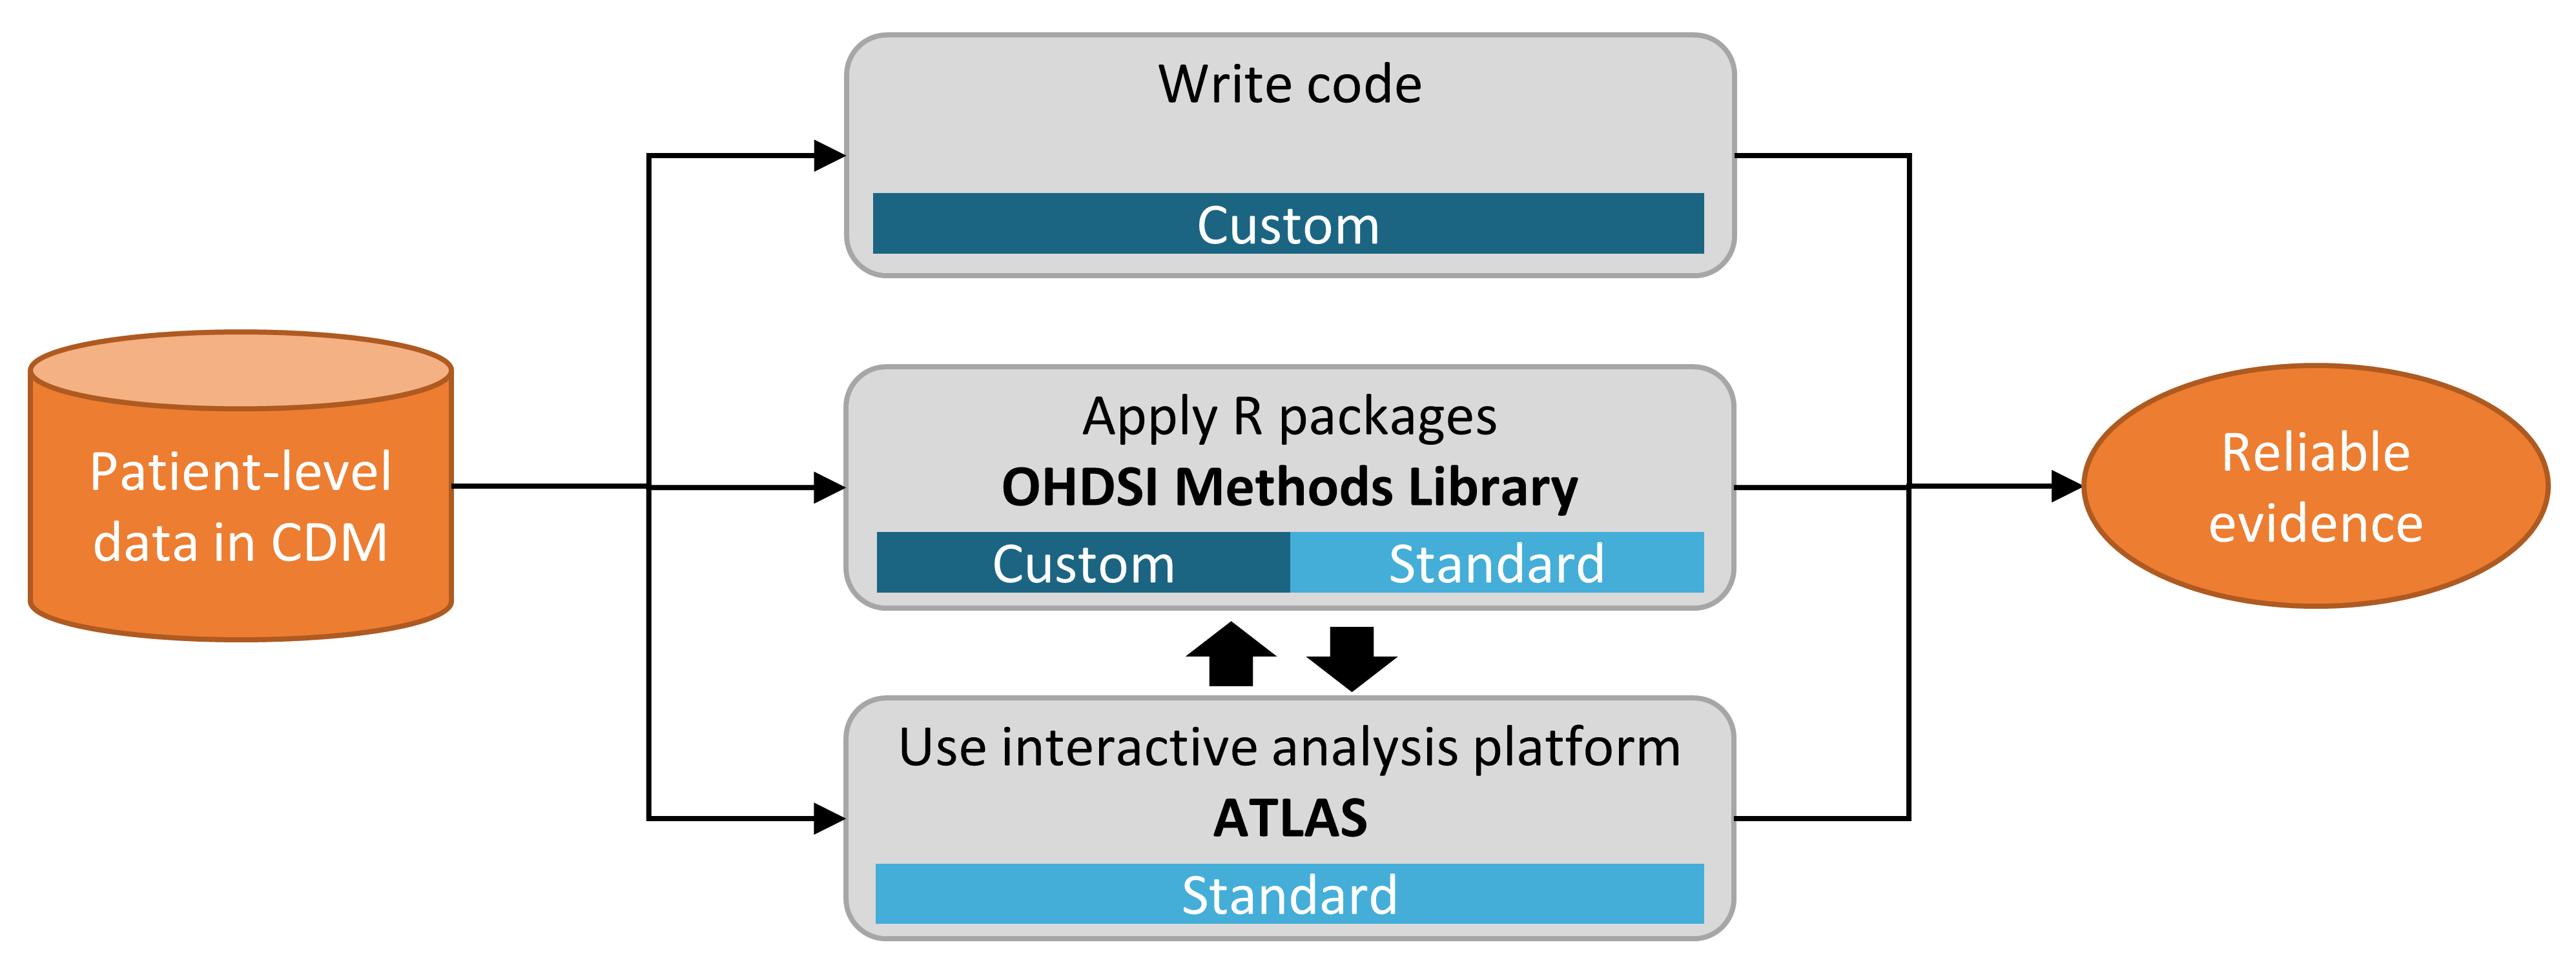
\includegraphics[width=0.9\linewidth]{images/OhdsiAnalyticsTools/implementations} 

}

\caption{Different ways to implement an analysis against data in the CDM.}\label{fig:implementations}
\end{figure}

We may choose to write our analysis as custom code, and not make use of
any of the tools OHDSI has to offer. One could write a de novo analysis
in R, SAS, or any other language. This provides the maximum flexibility,
and may in fact be the only option if the specific analysis is not
supported by any of our tools. However, this path requires a lot of
technical skill, time, and effort, and as the analysis increases in
complexity it becomes harder to avoid errors in the code.

An alternative is to develop the analysis in R, and make use of the
packages in the \href{https://ohdsi.github.io/MethodsLibrary/}{OHDSI
Methods Library}. At a minimum, one could use the
\href{https://ohdsi.github.io/SqlRender/}{SqlRender} and
\href{https://ohdsi.github.io/DatabaseConnector/}{DatabaseConnector}
packages described in more detail in Chapter \ref{SqlAndR} that allow
the same code to be executed on various database platforms, such as
PostgreSQL, SQL Server, and Oracle. Other packages such as
\href{https://ohdsi.github.io/CohortMethod/}{CohortMethod} and
\href{https://ohdsi.github.io/PatientLevelPrediction/}{PatientLevelPrediction}
offer R functions for advanced analytics against the CDM that can be
called on in one's code. This still requires a lot of tecnhical
expertise, but by re-using the validated components of the Methods
Library we can be more efficient and error-free than when using
completely custom code.

The third approach relies on our interactive analysis platform
\href{https://github.com/OHDSI/Atlas/wiki}{ATLAS}, a web-based tool that
allows non-programmers to perform a wide range of analyses efficiently.
The downside is that some options may not be available.

ATLAS and the Methods Library are not independent. Some of the more
complicated analytics that can be invoked in ATLAS are executed through
calls to the packages in the Methods Library. Similarly, cohorts used in
the Methods Library are often designed in ATLAS.

\section{Analysis strategy}\label{analysis-strategy}

More or less independently of how we choose to implement our analysis is
the strategy that our analytics takes in answering specific questions.
Figure \ref{fig:strategies} highlights three strategies that are
employed in OHDSI.

\begin{figure}

{\centering 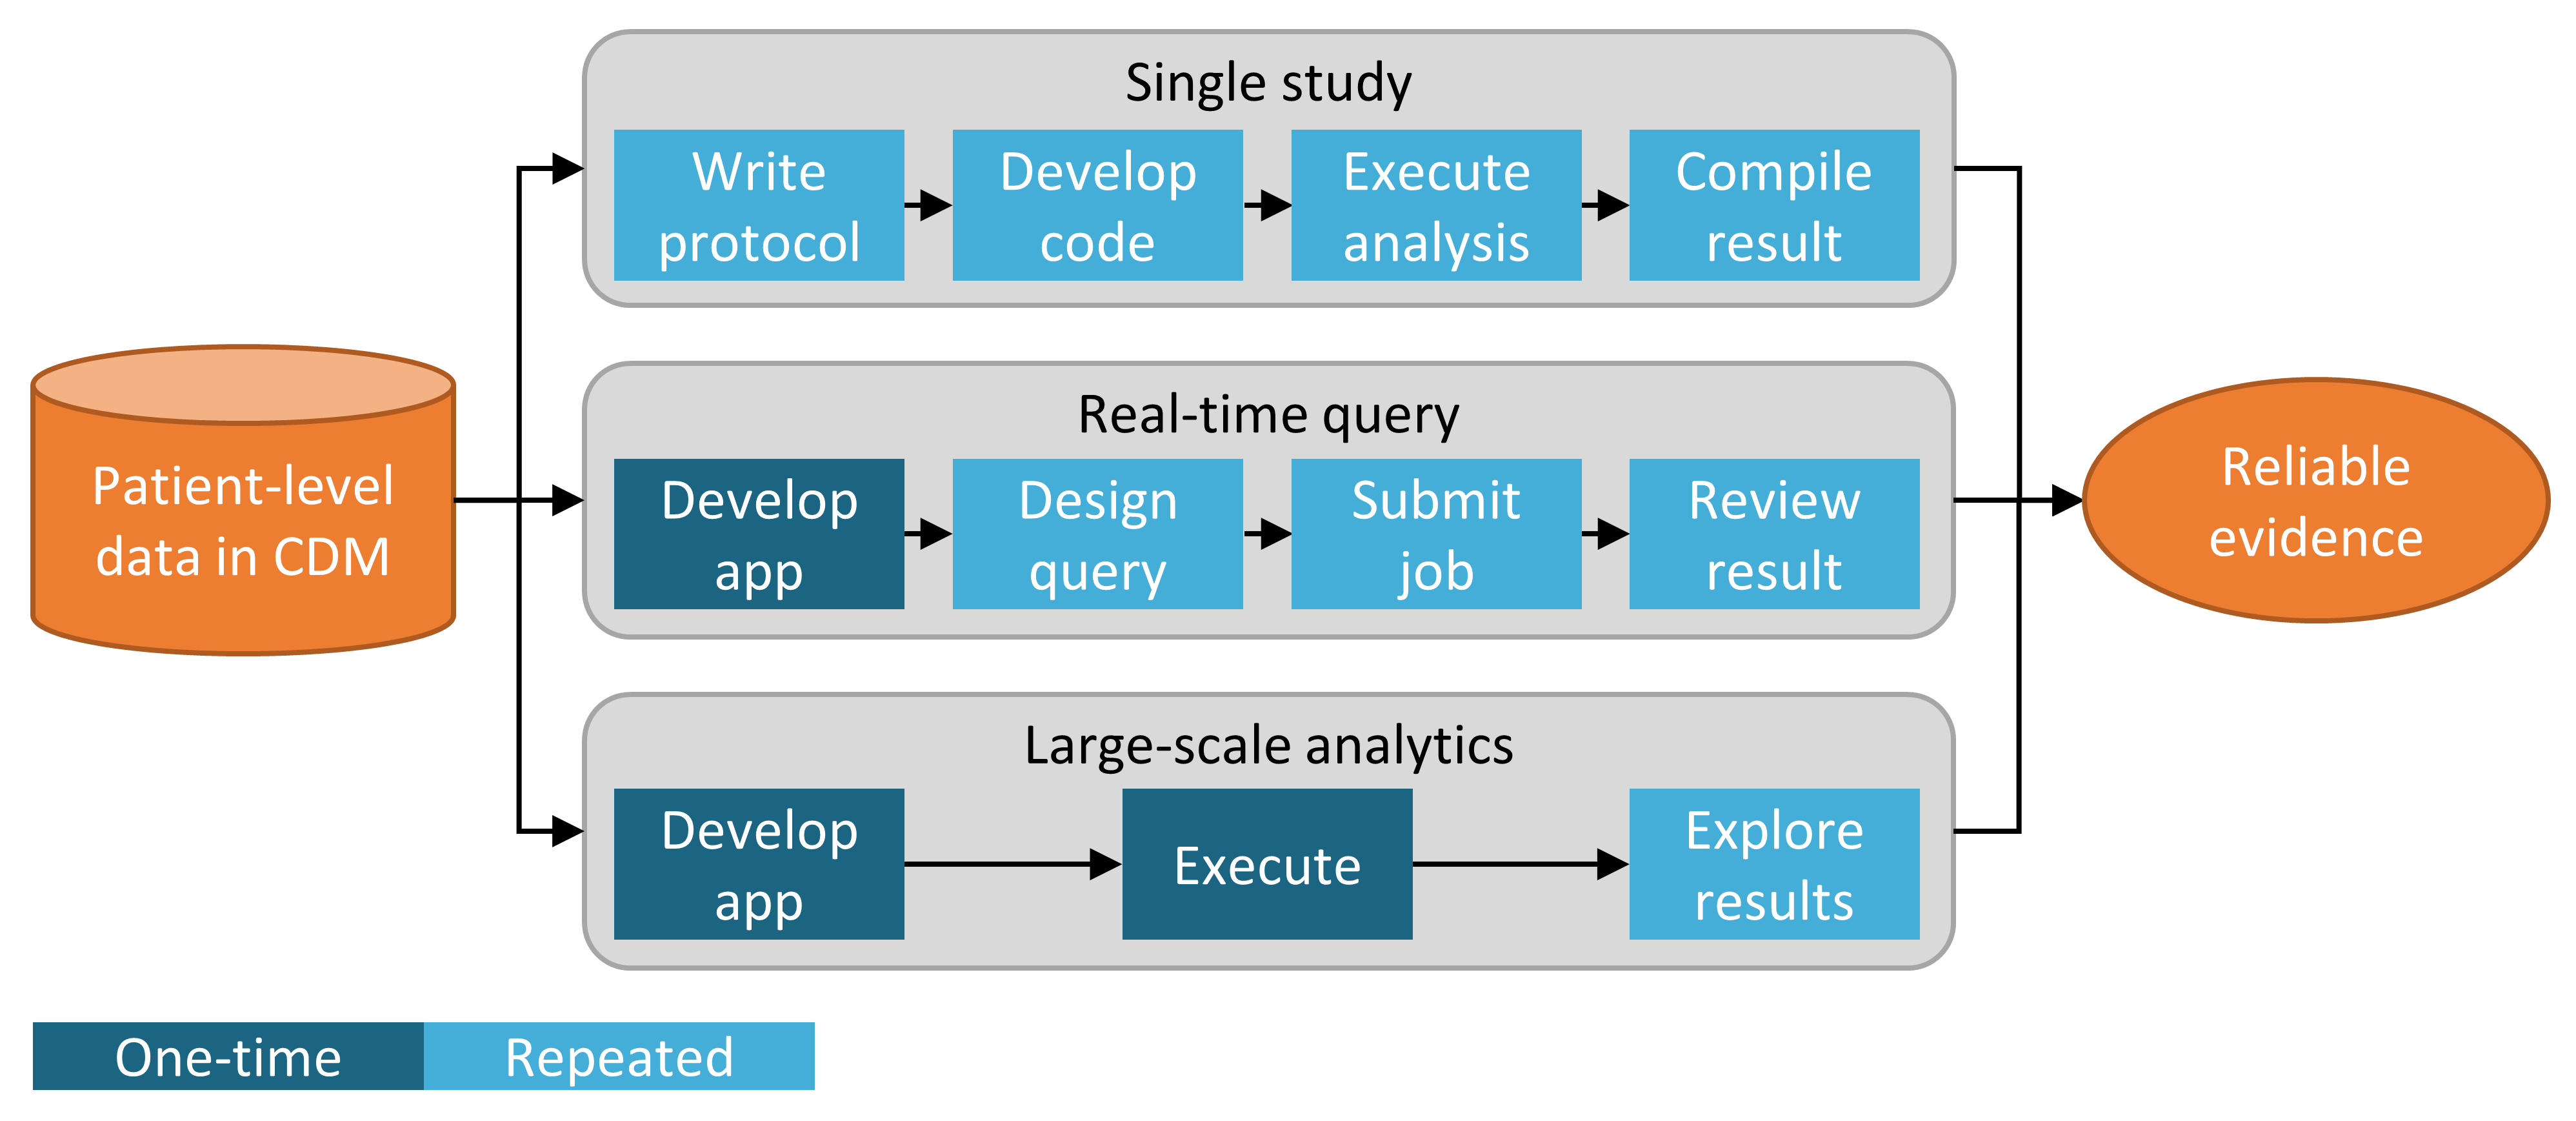
\includegraphics[width=0.9\linewidth]{images/OhdsiAnalyticsTools/strategies} 

}

\caption{Strategies for generating evidence for (clinical) questions.}\label{fig:strategies}
\end{figure}

The first strategy views every analysis as a single individual study.
The analysis must be pre-specified in a protocol, implemented as code,
executed against the data, after which the result can be compiled and
interpreted. For every question, all steps must be repeated. An example
of such an analysis is the OHDSI study into the risk of angioedema
associated with levetiracetam compared with phenytoin. \citep{duke_2017}
Here, a protocol was first written, analysis code using the OHDSI
Methods Library was developed and executed across the OHDSI network, and
results were compiled and disseminated in a journal publication.

The second strategy develops some app that allows users to answer a
specific class of questions in real time or near-real time. Once the app
has been developed, users can interactively define queries, submit them,
and view the results. An example is the cohort definition and generation
tool in ATLAS. This tool allows users to specify cohort definitions of
arbitrary complexity, and execute the definition against a database to
see how many people meet the various inclusion and exclusion criteria.

The third strategy similarly focuses on a class of questions, but then
attempts to exhaustively generate all the evidence for the questions
within the class. Users can then explore the evidence as needed, usually
through some viewer app. One example is the OHDSI study into the effects
of depression treatments \citep{schuemie_2018b}. In this study all
depression treatments are compared for a large set of outcomes of
interest across four large observational databases. The full set of
results, including 17,718 empirically calibrated hazard ratios along
with extensive study diagnostics, is available in an interactive web app
\footnote{\url{http://data.ohdsi.org/SystematicEvidence/}}.

\section{ATLAS}\label{atlas}

ATLAS is a web-based tool that must run on a server with access to the
patient-level data in the CDM. To directly run the analyses against the
data, ATLAS must therefore be installed behind your organization's
firewall. However, there is also a public ATLAS \footnote{\url{http://www.ohdsi.org/web/atlas}},
and although this ATLAS instance only has access to a small simulated
dataset, it can still be used for many purposes. For example, it is
possible to fully define an effect estimation of prediction study in the
public ATLAS, and automatically generate the R code for executing the
study.

\begin{figure}

{\centering 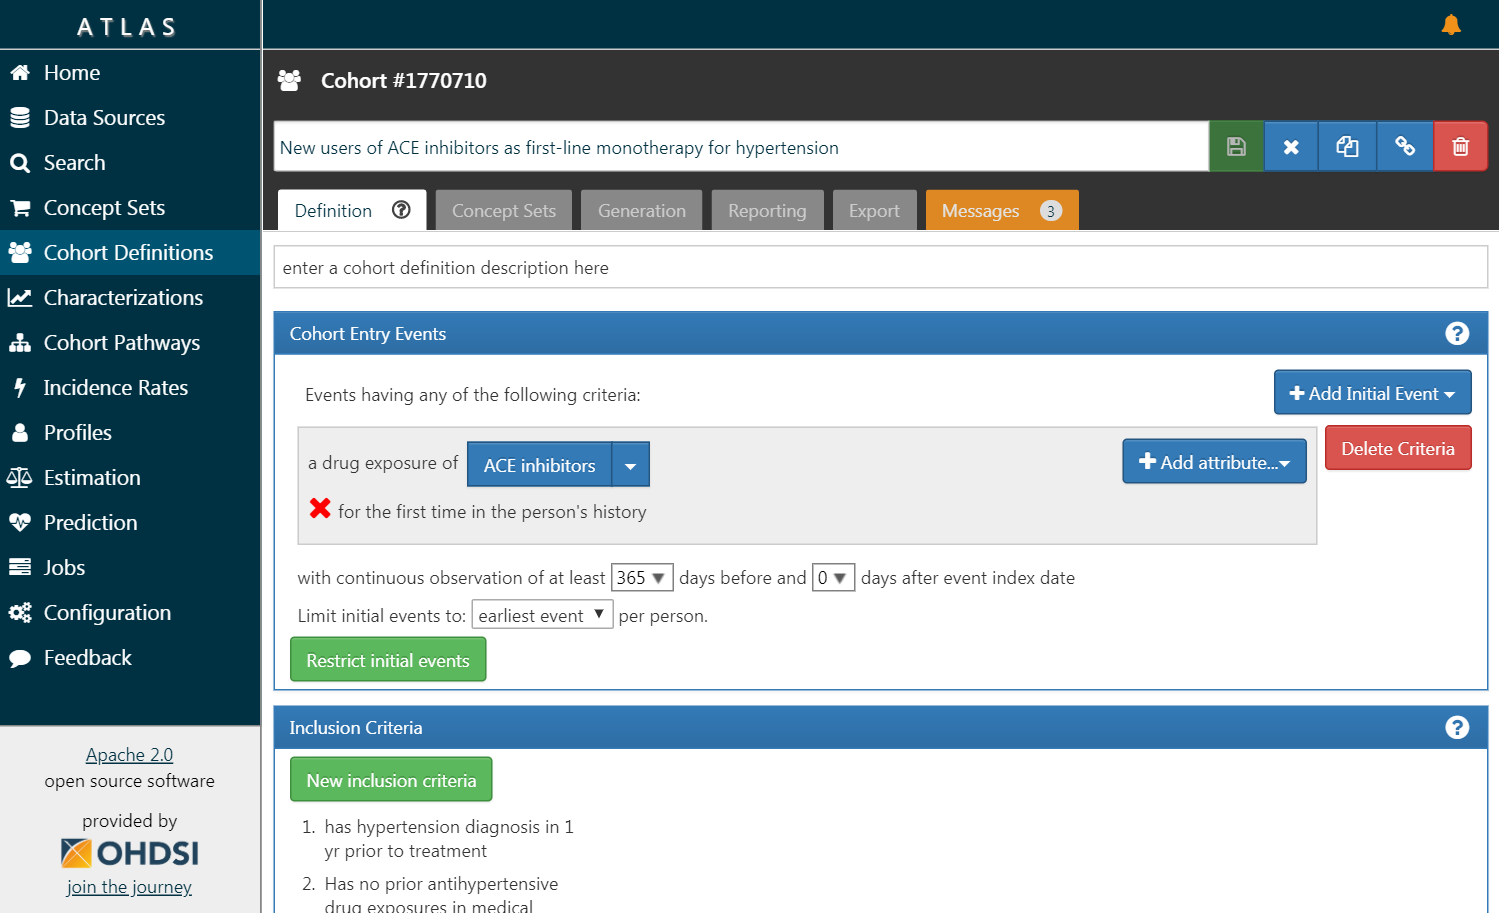
\includegraphics[width=1\linewidth]{images/OhdsiAnalyticsTools/atlas} 

}

\caption{ATLAS user interface.}\label{fig:atlas}
\end{figure}

A screenshot of ATLAS is provided in Figure \ref{fig:atlas}. On the left
is a navigation bar showing the various functions provided by ATLAS:

\begin{description}
\tightlist
\item[Data Sources]
Data sources provides the capability review descriptive, standardized
reporting for each of the data sources that you have configured within
your Atlas platform. This feature uses the large-scale analytics
strategy: all descriptives have been pre-computed. Data sources is
discussed in Chapter \ref{Characterization}.
\item[Vocabulary Search]
Atlas provides the ability to search and explore the OMOP standardized
vocabulary to understand what concepts exist within those vocabularies
and how to apply those concepts in your standardized analysis against
your data sources. This feature is discussed in Chapter
\ref{StandardizedVocabularies}.
\item[Concept Sets]
Concept sets is the ability to create your own lists of codes that you
are going to use throughout your standardized analyses so by searching
the vocabulary and identifying the sets of terms that you're interested
in you can save those and reuse them in all of your analyses.
\item[Cohort Definitions]
Cohort definitions is the ability to construct a set of persons who
satisfy one or more criteria for a duration of time and these cohorts
can then serve as the basis of inputs for all of your subsequent
analyses. This feature is discussed in Chapter \ref{Cohorts}.
\item[Characterizations]
Characterisations is an analytic capability that allows you to look at
one or more cohorts that you've defined and to summarize characteristics
about those patient populations. This feature uses the real-time query
strategy, and is discussed in Chapter \ref{Characterization}.
\item[Cohort Pathways]
Cohort pathways is an analytic tool that allows you to look at the
sequence of clinical events that occur within one or more populations.
This feature uses the real-time query strategy, and is discussed in
Chapter \ref{Characterization}.
\item[Incidence Rates]
Incidence rates is a tool that allows you to estimate the incidence of
outcomes within target populations of interest. This feature uses the
real-time query strategy, and is discussed in Chapter
\ref{Characterization}.
\item[Profiles]
Profiles is a tool that allows you to explore an individual patients
longitudinal observational data to summarize what is going on within a
given individual. This feature uses the real-time query strategy.
\item[Population Level Estimation]
Estimation is a capability to allow you to conduct population level
effect estimation studies using a comparative cohort design whereby
comparisons between one or more target and comparator cohorts can be
explored for a series of outcomes. This feature can be said to implement
the real-time query strategy, as no coding is required, and is discussed
in Chapter \ref{PopulationLevelEstimation}.
\item[Patient Level Prediction]
Prediction is a capability to allow you to apply machine learning
algorithms to conduct patient level prediction analyses whereby you can
predict an outcome within any given target exposures. This feature can
be said to implement the real-time query strategy, as no coding is
required, and is discussed in Chapter \ref{PatientLevelPrediction}.
\item[Jobs]
Select the ``jobs'' menu item to explore jobs that are running in the
background for long running processes such as generating a cohort or
computing cohort reports.
\item[Configuration]
Select the ``configuration'' menu item to review the data sources that
have been configured in the source configuration section.
\item[Feedback]
This will take you to the issue log for Atlas so that you can log a new
issue or to search through existing issues. If you have ideas for new
features or enhancements, this is also a place note these for the
development community.
\end{description}

\subsection{Security}\label{security}

\subsection{Documentation}\label{documentation}

\subsection{System requirements}\label{system-requirements}

\subsection{How to install}\label{how-to-install}

\section{Methods Library}\label{methods-library}

The \href{https://ohdsi.github.io/MethodsLibrary/}{OHDSI Methods
Library} is the collection of open source R packages show in Figure
\ref{fig:methodsLibrary}.

\begin{figure}

{\centering 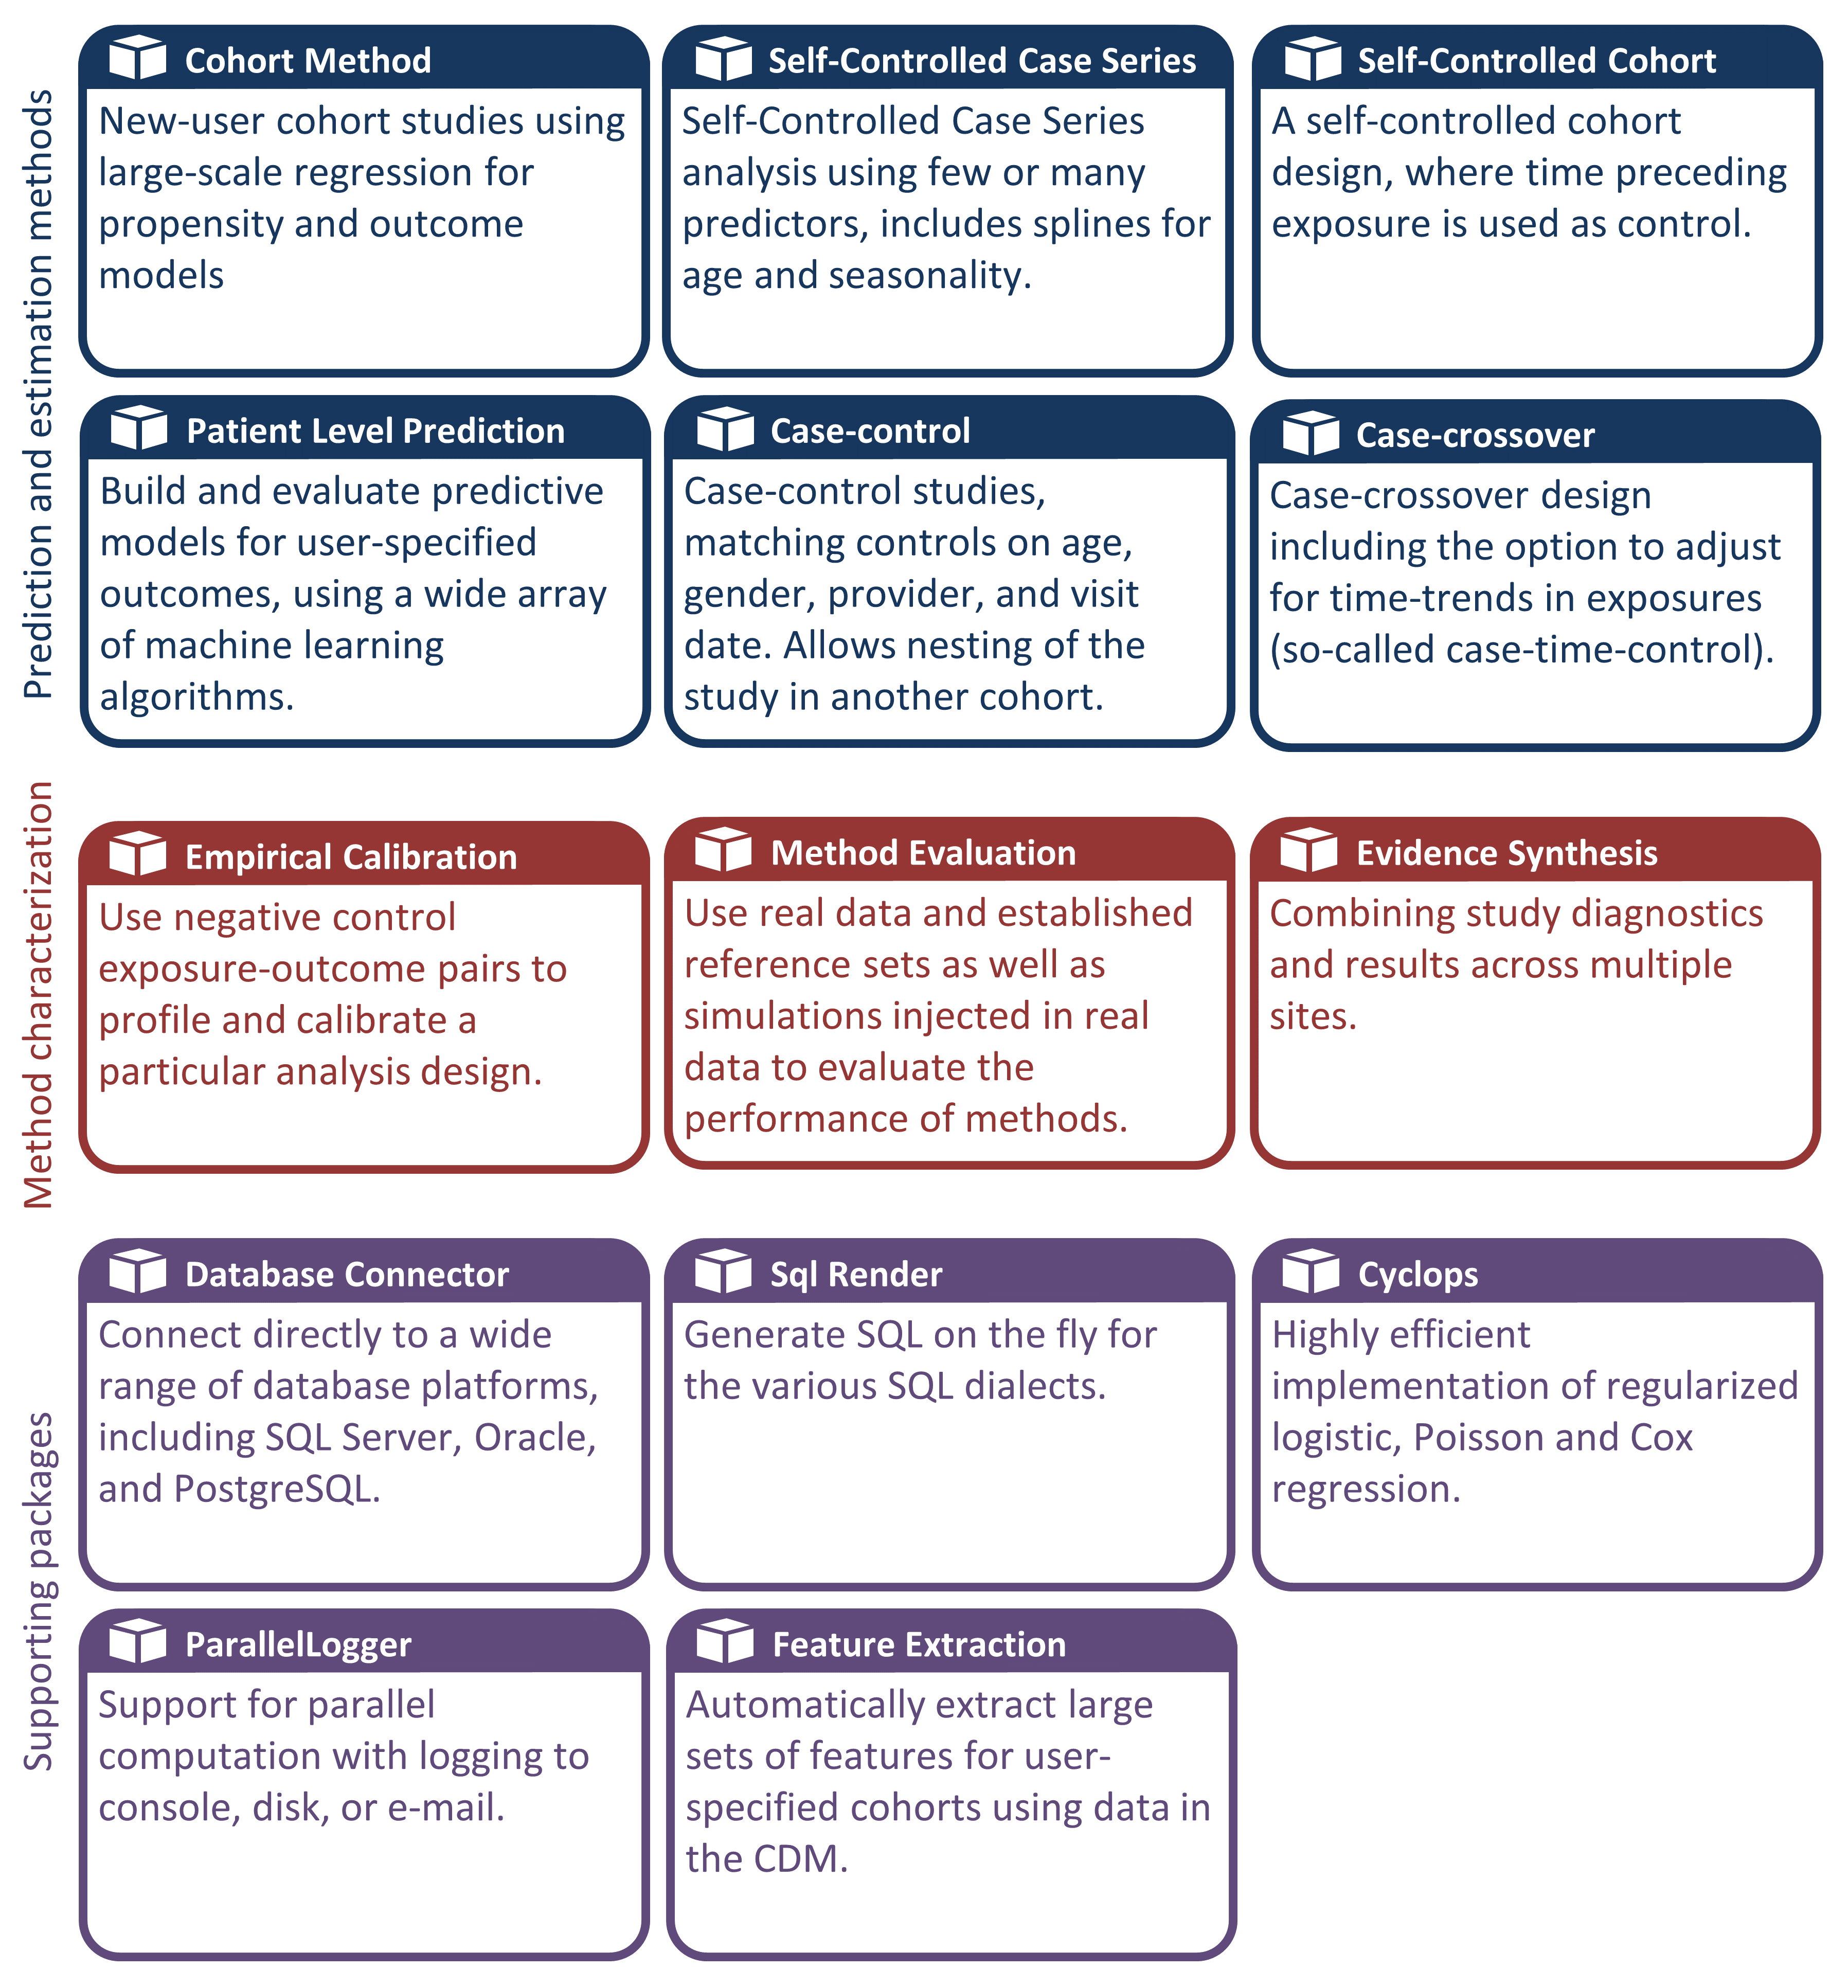
\includegraphics[width=1\linewidth]{images/OhdsiAnalyticsTools/methodsLibrary} 

}

\caption{Packages in the OHDSI Methods Library.}\label{fig:methodsLibrary}
\end{figure}

The packages offer R functions that together can be used to perform an
observation study from data to estimates and supporting statistics,
figures, and tables. The packages interact directly with observational
data in the CDM, and can be used simply to provide cross-platform
compatibility to completely custom analyses as described in Chapter
\ref{SqlAndR}, or can provide advanced standardized analytics for
population characterization (Chapter \ref{Characterization}),
population-level causal effect estimation (Chapter
\ref{PopulationLevelEstimation}), and patient-level prediction (Chapter
\ref{PatientLevelPrediction}). The Methods Library supports best
practices for use of observational data as learned from previous and
ongoing research, such as transparency, reproducibility, as well as
measuring of the operating characteristics of methods in a particular
context and subsequent empirical calibration of estimates produced by
the methods.

The Methods Library has already been used in many published clinical
studies
\citep{boland_2017, duke_2017, ramcharran_2017, weinstein_2017, wang_2017, ryan_2018, vashisht_2018, yuan_2018, johnston_2019},
as well as methodological studies
\citep{schuemie_2014, schuemie_2016, reps2018, tian_2018, schuemie_2018, schuemie_2018b, reps_2019}.
Great care is taken to ensure the validity of the Methods Library, as
described in Chapter \ref{SoftwareValidity}.

\subsection{Support for large-scale
analytics}\label{support-for-large-scale-analytics}

One key feature incorporated in all packages is the ability to
efficiently run many analyses. For example, when performing
population-level estimation, the CohortMethod package allows for
computing effect-size estimates for many exposures and outcomes, using
various analysis settings, and the package will automatically choose the
optimal path to compute all the required artifacts. Steps that can be
re-used, such as extraction of covariates, or fitting a propensity
model, will be executed only once. Where possible, computations will
take place in parallel to maximuze the use of computational resources.

This feature allows for large-scale analytics, answering many questions
at once, and is also essential for including control hypotheses
(e.g.~negative controls) to measure the operating characteristics of our
methods, and perform empirical calibration as described in Chapter
\ref{MethodValidity}.

\subsection{Support for big data}\label{BigDataSupport}

The Methods Library is also designed to run against very large databases
and be able to perform computations involving large amounts of data.
This achieved in three ways:

\begin{enumerate}
\def\labelenumi{\arabic{enumi}.}
\tightlist
\item
  Most data manipulation is performed on the database server. An
  analysis usually only requires a small fraction of the entire data in
  the database, and the Methods Library, through the SqlRender and
  DatabaseConnector packages, allows for advanced operations to be
  performed on the server to preprocess and extract the relevant data.
\item
  Large local data objects are stored in a memory-efficient manner. For
  the data that is downloaded to the local machine, the Methods Library
  uses the \href{https://cran.r-project.org/web/packages/ff}{ff} package
  to store and work with large data objects. This allows us to work with
  data much larger than fits in memory.
\item
  High-performance computing is applied where needed. For example, the
  \href{https://ohdsi.github.io/Cyclops/}{Cyclops} package implements a
  highly efficient regression engine that is used throughout the Methods
  Library to perform large-scale regressions (large number of variables,
  large number of observations) that would not be possible to fit
  otherwise.
\end{enumerate}

\subsection{Documentation}\label{documentation-1}

R provides a standard way of documenting package. Each package has a
\emph{package manual} that documents every function and data set in the
package. All package manuals are available online through the Methods
Library website \footnote{\url{https://ohdsi.github.io/MethodsLibrary}},
through the package GitHub repositories, and for those packages
available through CRAN they can be found in CRAN. Furtermore, from
within R the package manual can be consulted by using the question mark.
For example, after loading the DatabaseConnector package, typing the
command \texttt{?connect} brings up the documentation on the ``connect''
function.

In addition to the package manual, many packages provide
\emph{vignettes}. Vignettes are long-form documentation that describe
how a package can be used to perform certain tasks. For example, one
vignette \footnote{\url{https://ohdsi.github.io/CohortMethod/articles/MultipleAnalyses.html}}
describes how to perform multiple analyses efficiently using the
CohortMethod package. Vignettes can also be found through the Methods
Library website , through the package GitHub repositories, and for those
packages available through CRAN they can be found in CRAN.

\subsection{System requirements}\label{system-requirements-1}

Two computing environments are relevant when discussing the system
requirements: The database server, and the analytics workstation.

The database server must hold the observational healthcare data in CDM
format. The Methods Library supports a wide array of database management
systems including traditional database systems (PostgreSQL, Microsoft
SQL Server, and Oracle), parallel data warehouses (Microsoft APS, IBM
Netezza, and Amazon RedShift), as well as Big Data platforms (Hadoop
through Impala, and Google BigQuery).

The analytics workstation is where the Methods Library is installed and
run. This can either be a local machine, such as someone's laptop, or a
remote server running RStudio Server. In all cases the requiments are
that R is installed, preferrably together with RStudio. The Methods
Library also requires that Java is installed. The analytics workstation
should also be able to connect to the database server, specifically, any
firewall between them should have the database server access ports
opened the the workstation. Some of the analytics can be computationally
intensive, so having multiple processing cores and ample memory can help
speed up the analyses. We recommend having at least four cores and 16
gigabytes of memory.

\subsection{How to install}\label{how-to-install-1}

Here are the steps for installing the required environment to run the
OHDSI R packages. Four things needs to be installed:

\begin{enumerate}
\def\labelenumi{\arabic{enumi}.}
\tightlist
\item
  \textbf{R} is a statistical computing environment. It comes with a
  basic user interface that is primarily a command-line interface.
\item
  \textbf{RTools} is a set of programs that is required on Windows to
  build R packages from source.
\item
  \textbf{RStudio} is an IDE (Integrated Development Environment) that
  makes R easier to use. It includes a code editor, debugging and
  visualization tools. Please use it to obtain a nice R experience.
\item
  \textbf{Java} is a computing environment that is needed to run some of
  the components in the OHDSI R packages, for example those needed to
  connect to a database.
\end{enumerate}

Below we describe how to install each of these in a Windows environment.

\BeginKnitrBlock{rmdimportant}
In Windows, both R and Java come in 32-bit and 64-bits architectures. If
you install R in both architectures, you \textbf{must} also install Java
in both architectures. It is recommended to only install the 64-bit
version of R.
\EndKnitrBlock{rmdimportant}

\textbf{Installing R}

\begin{enumerate}
\def\labelenumi{\arabic{enumi}.}
\tightlist
\item
  Go to \url{https://cran.r-project.org/}, click on ``Download R for
  Windows'', then ``base'', then click the Download link indicated in
  Figure \ref{fig:downloadR}.
\end{enumerate}

\begin{figure}

{\centering 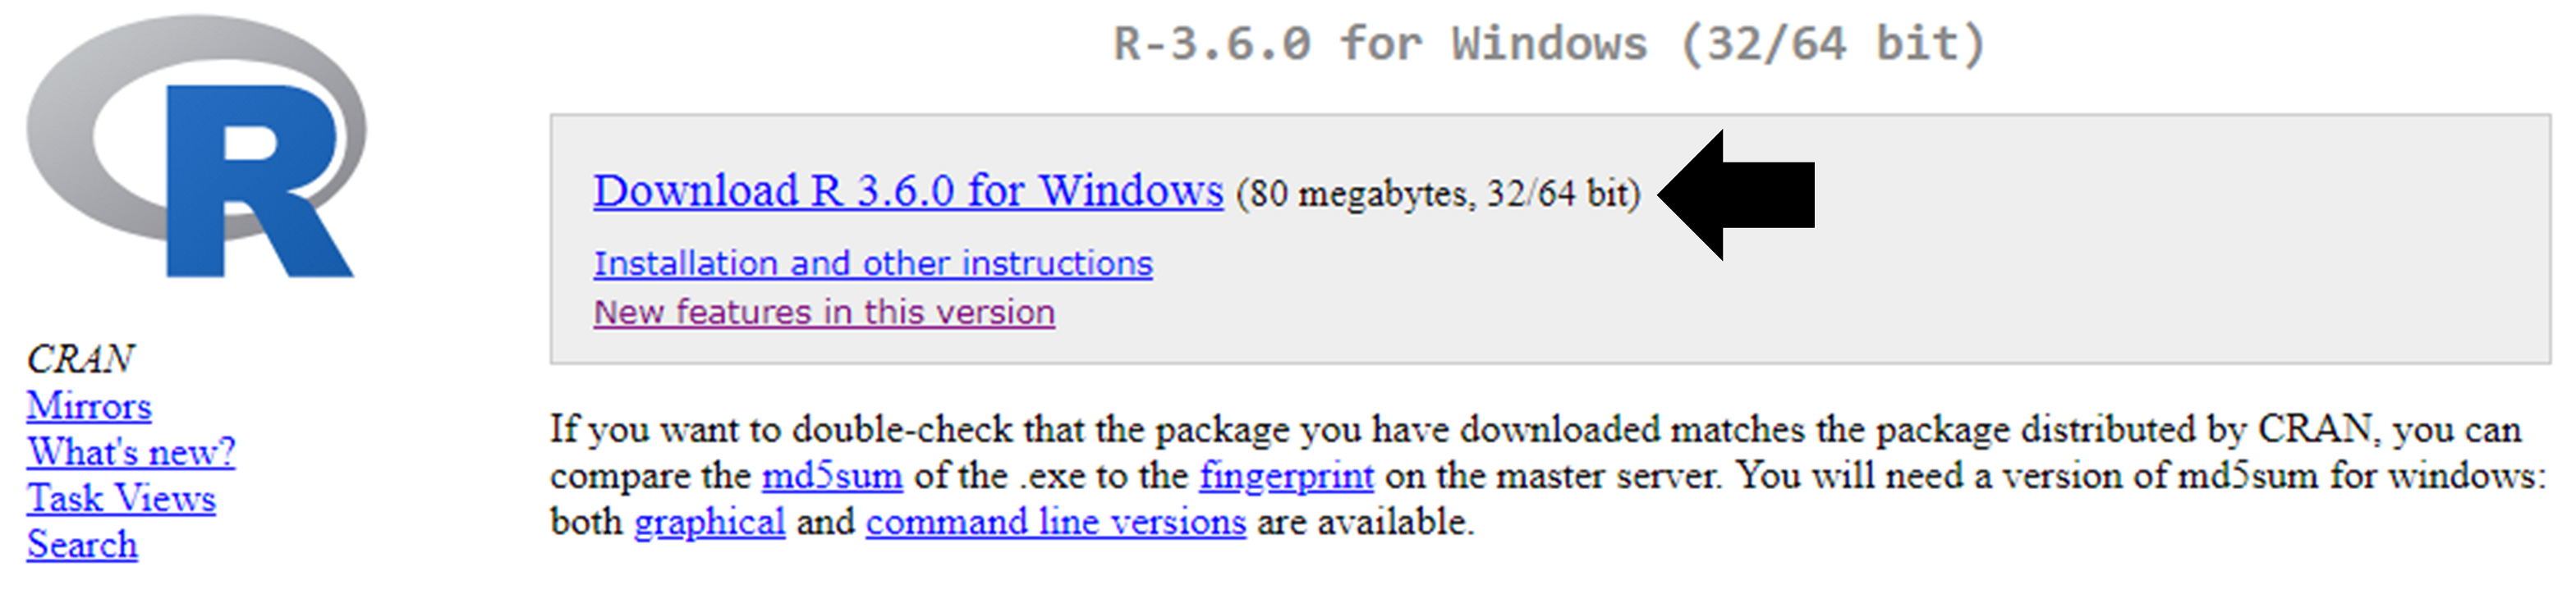
\includegraphics[width=1\linewidth]{images/OhdsiAnalyticsTools/downloadR} 

}

\caption{Downloading R from CRAN.}\label{fig:downloadR}
\end{figure}

\begin{enumerate}
\def\labelenumi{\arabic{enumi}.}
\setcounter{enumi}{1}
\tightlist
\item
  After the download has completed, run the installer. Use the default
  options everywhere, with two exceptions: First, it is better not to
  install into program files. Instead, just make R a subfolder of your C
  drive as shown in Figure \ref{fig:rDestination}. Second, to avoid
  problems due to differing architectures between R and Java, disable
  the 32-bit architecture as shown in Figure \ref{fig:no32Bits}.
\end{enumerate}

\begin{figure}

{\centering 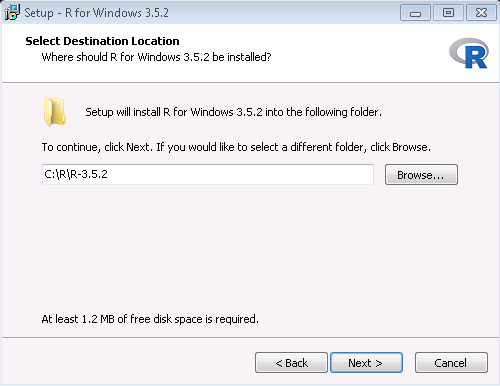
\includegraphics[width=0.8\linewidth]{images/OhdsiAnalyticsTools/rDestination} 

}

\caption{Settings the destination folder for R.}\label{fig:rDestination}
\end{figure}

\begin{figure}

{\centering 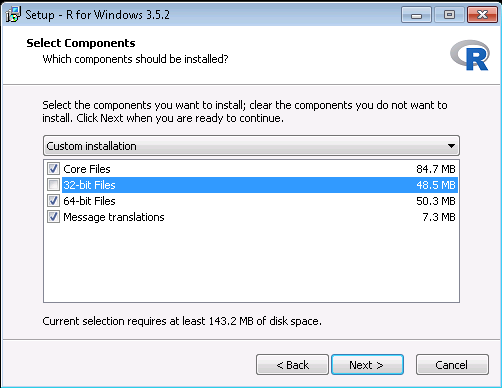
\includegraphics[width=0.8\linewidth]{images/OhdsiAnalyticsTools/no32Bits} 

}

\caption{Disabling the 32-bit version of R.}\label{fig:no32Bits}
\end{figure}

Once completed, you should be able to select R from your Start Menu.

\textbf{Installing RTools}

\begin{enumerate}
\def\labelenumi{\arabic{enumi}.}
\item
  Go to \url{https://cran.r-project.org/}, click on ``Download R for
  Windows'', then ``Rtools'', and select the very latest version of
  RTools to download.
\item
  After downloading has completed run the installer. Select the default
  options everywhere.
\end{enumerate}

\textbf{Installing RStudio}

\begin{enumerate}
\def\labelenumi{\arabic{enumi}.}
\tightlist
\item
  Go to \url{https://www.rstudio.com/}, select ``Download RStudio'' (or
  the ``Download'' button under ``RStudio''), opt for the free version,
  and download the installer for Windows as shown in Figure
  \ref{fig:downloadRStudio}.
\end{enumerate}

\begin{figure}

{\centering 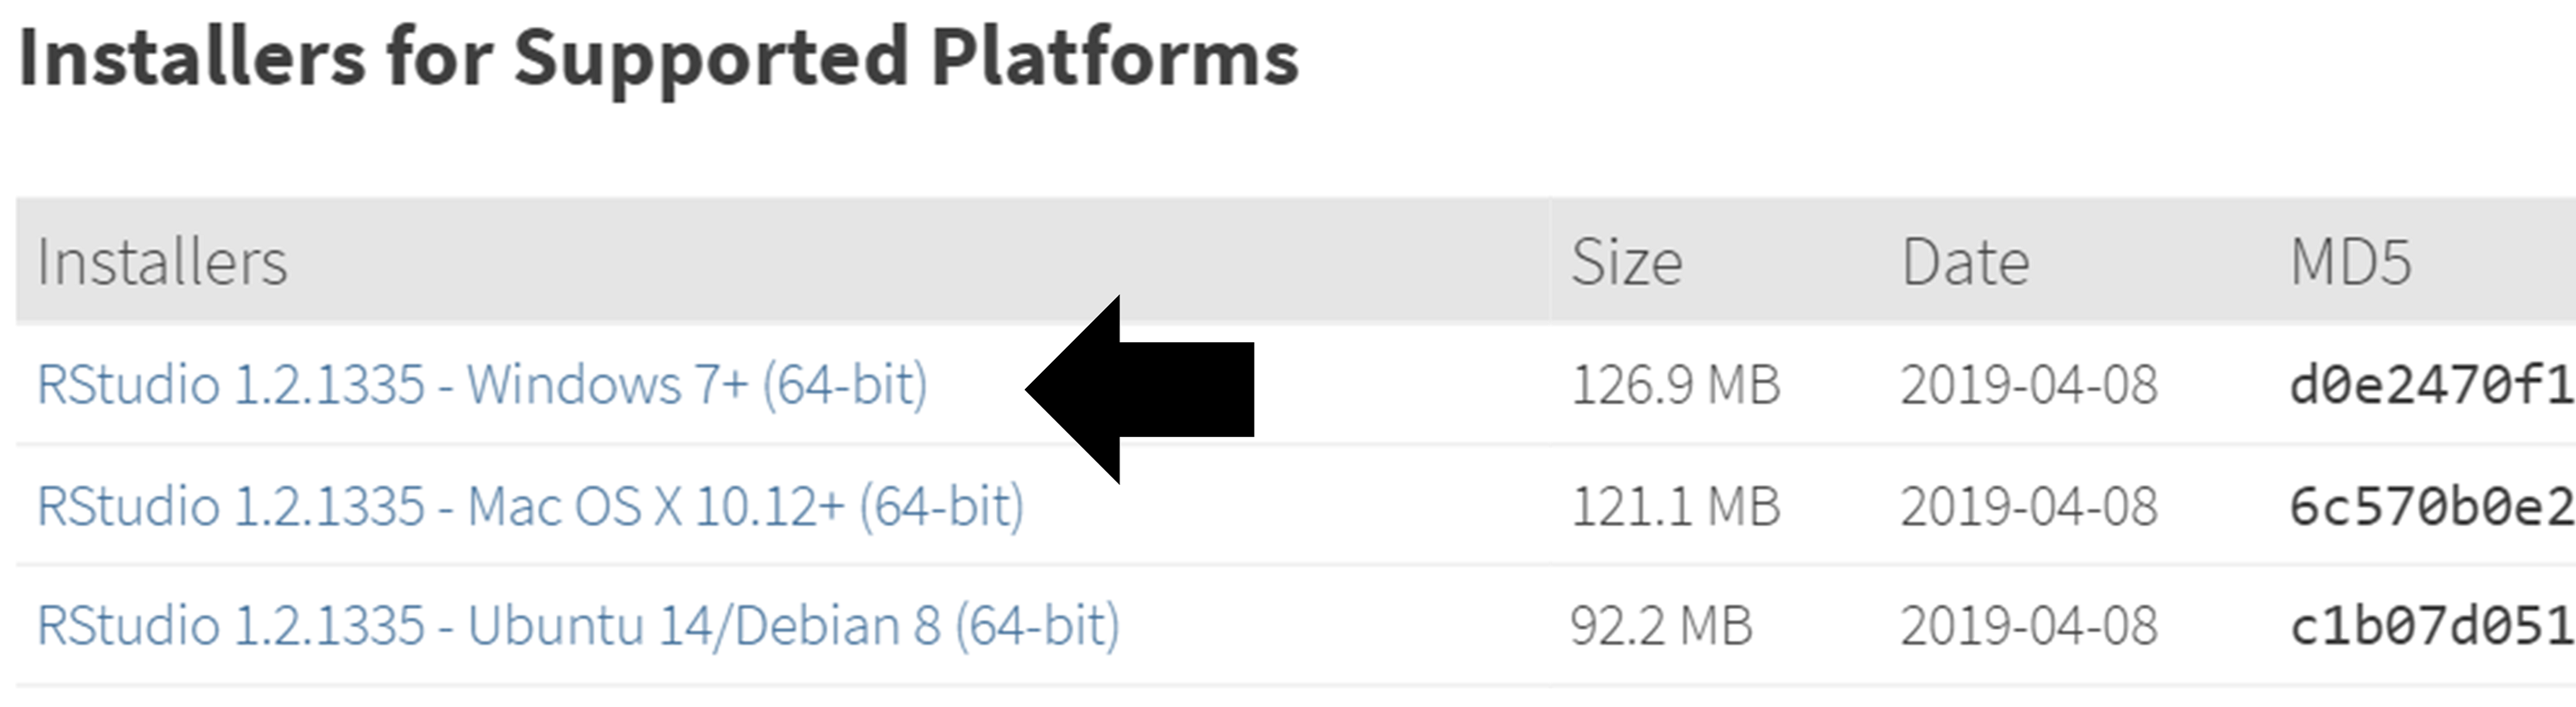
\includegraphics[width=1\linewidth]{images/OhdsiAnalyticsTools/downloadRStudio} 

}

\caption{Downloading RStudio.}\label{fig:downloadRStudio}
\end{figure}

\begin{enumerate}
\def\labelenumi{\arabic{enumi}.}
\setcounter{enumi}{1}
\tightlist
\item
  After downloading, start the installer, and use the default options
  everywhere.
\end{enumerate}

\section{Installing Java}\label{installing-java}

\begin{enumerate}
\def\labelenumi{\arabic{enumi}.}
\tightlist
\item
  Go to \url{https://java.com/en/download/manual.jsp}, and select the
  Windows 64-bit installer as shown in Figure \ref{fig:downloadJava}. If
  you also installed the 32-bit version of R, you \emph{must} also
  install the other (32-bit) version of Java.
\end{enumerate}

\begin{figure}

{\centering 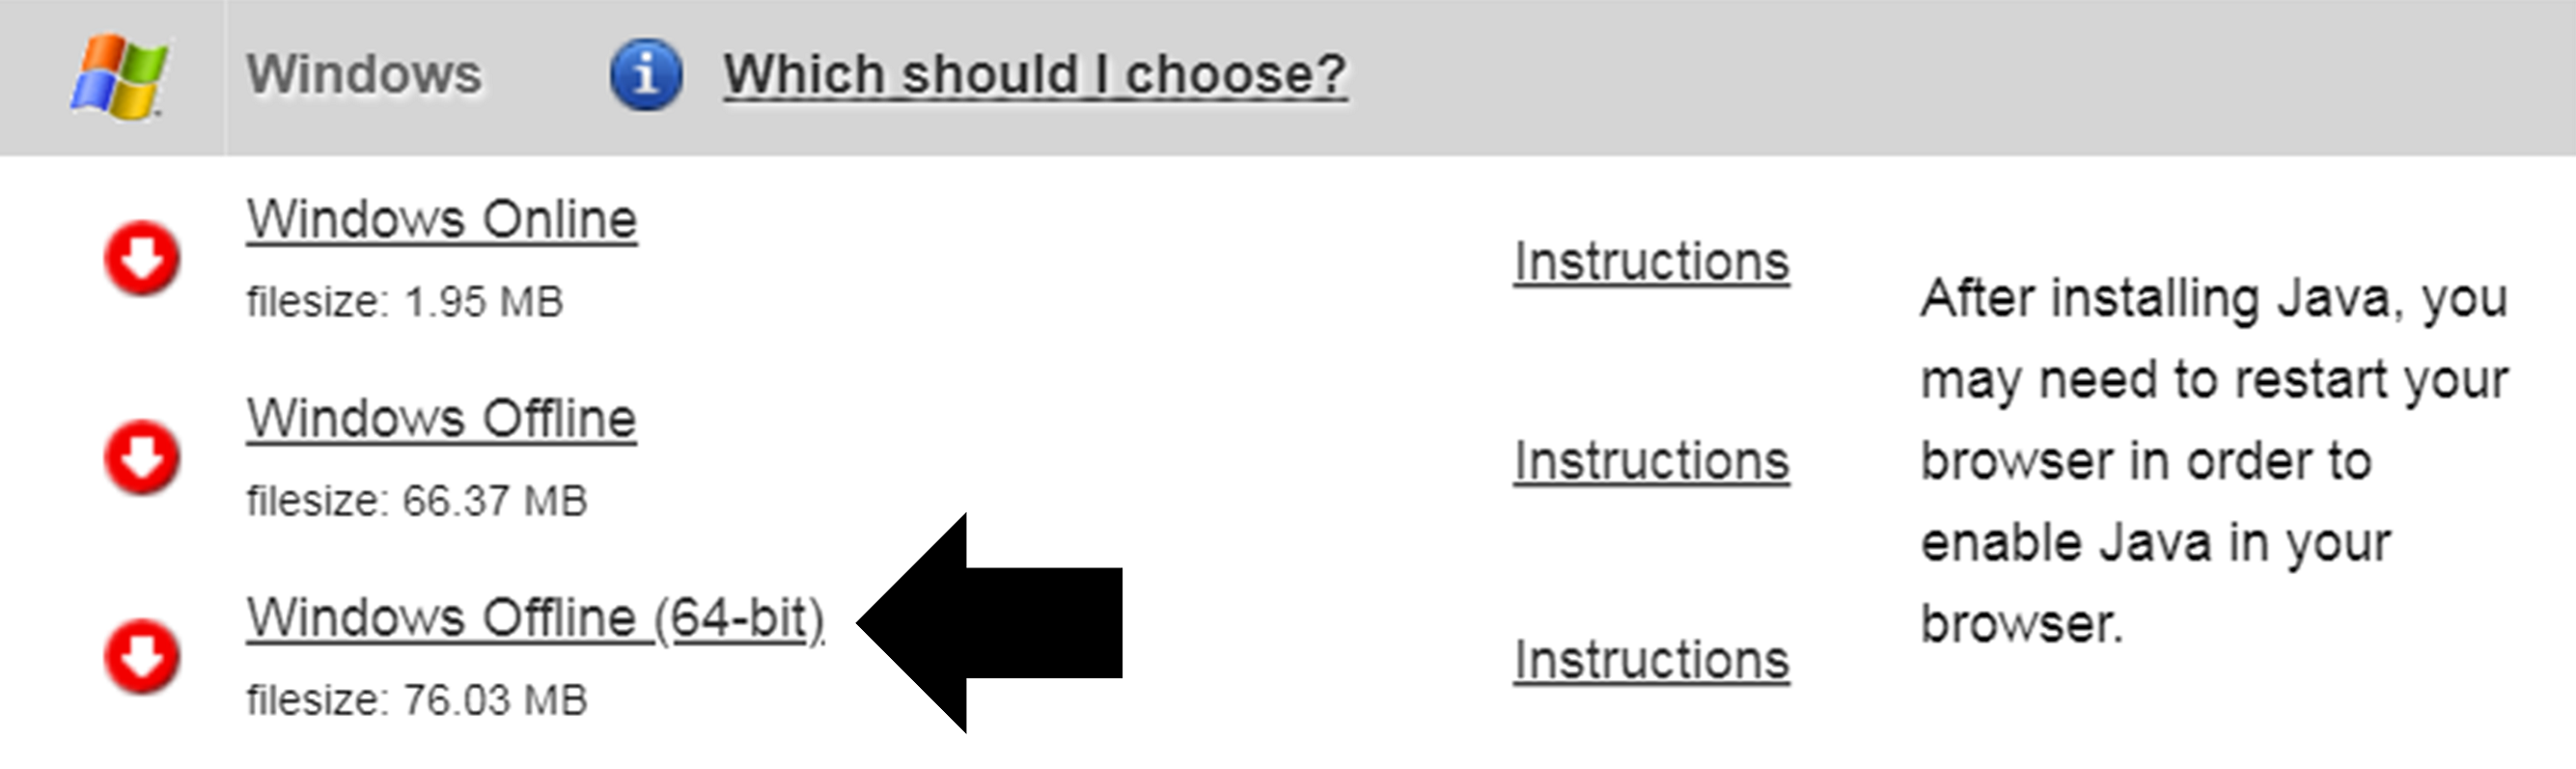
\includegraphics[width=1\linewidth]{images/OhdsiAnalyticsTools/downloadJava} 

}

\caption{Downloading Java.}\label{fig:downloadJava}
\end{figure}

\begin{enumerate}
\def\labelenumi{\arabic{enumi}.}
\setcounter{enumi}{1}
\tightlist
\item
  After downloading just run the installer.
\end{enumerate}

\textbf{Verifying the installation}

You should now be ready to go, but we should make sure. Start R-studio,
and type

\begin{Shaded}
\begin{Highlighting}[]
\KeywordTok{install.packages}\NormalTok{(}\StringTok{"SqlRender"}\NormalTok{)}
\KeywordTok{library}\NormalTok{(SqlRender)}
\KeywordTok{translate}\NormalTok{(}\StringTok{"SELECT TOP 10 * FROM person;"}\NormalTok{, }\StringTok{"postgresql"}\NormalTok{)}
\end{Highlighting}
\end{Shaded}

\begin{verbatim}
## [1] "SELECT  * FROM person LIMIT 10;"
\end{verbatim}

This function uses Java, so if all goes well we know both R and Java
have been installed correctly!

Another test is to see if source packages can be built. Run the
following R code to install the \texttt{CohortMethod} package from the
OHDSI GitHub repository:

\begin{Shaded}
\begin{Highlighting}[]
\KeywordTok{install.packages}\NormalTok{(}\StringTok{"drat"}\NormalTok{)}
\NormalTok{drat}\OperatorTok{::}\KeywordTok{addRepo}\NormalTok{(}\StringTok{"OHDSI"}\NormalTok{)}
\KeywordTok{install.packages}\NormalTok{(}\StringTok{"CohortMethod"}\NormalTok{)}
\end{Highlighting}
\end{Shaded}

\section{Integrated solutions}\label{integrated-solutions}

BroadSea?

\chapter{SQL and R}\label{SqlAndR}

\emph{Chapter leads: Martijn Schuemie \& Peter Rijnbeek}

The Common Data Model (CDM) is a relational database model (all data is
represented as records in tables that have fields), which means that the
data will typically be stored in a relational database using a software
platform like PostgreSQL, Oracle, or Microsoft SQL Server. The various
OHDSI tools such as ATLAS and the Methods Library work by querying the
database behind the scene, but we can also query the database directly
ourselves if we have appropriate access rights. The main reason to do
this is to perform analyses that currently are not supported by any
existing tool. However, directly querying the database also comes with
greater risk of making mistakes, as the OHDSI tools are often designed
to help guide the user to appropriate analysis of the data, and direct
queries do not provide such guidance.

The standard language for querying relational databases is SQL
(Structured Query Language), which can be used both to query the
database as well as to make changes to the data. Although the basic
commands in SQL are indeed standard, meaning the same across software
platforms, each platform has its own dialect, with subtle changes. For
example, to retrieve the top 10 rows of the PERSON table on SQL Server
one would type:

\begin{Shaded}
\begin{Highlighting}[]
\KeywordTok{SELECT}\NormalTok{ TOP }\DecValTok{10}\NormalTok{ * }\KeywordTok{FROM}\NormalTok{ person;}
\end{Highlighting}
\end{Shaded}

Whereas the same query on PostgreSQL would be:

\begin{Shaded}
\begin{Highlighting}[]
\KeywordTok{SELECT}\NormalTok{ * }\KeywordTok{FROM}\NormalTok{ person }\KeywordTok{LIMIT} \DecValTok{10}\NormalTok{;}
\end{Highlighting}
\end{Shaded}

In OHDSI, we would like to be agnostic to the specific dialect a
platform uses; We would like to `speak' the same SQL language across all
OHDSI databases. For this reason OHDSI developed the
\href{https://ohdsi.github.io/SqlRender/}{SqlRender} package, an R
package that can translate from one standard dialect to any of the
supported dialects that will be discussed later in this chapter. This
standard dialect - \textbf{OHDSI SQL} - is mainly a subset of the SQL
Server SQL dialect. The example SQL statements provided throughout this
chapter will all use OHDSI SQL.

Each database platform also comes with its own software tools for
querying the database using SQL. In OHDSI we developed the
\href{https://ohdsi.github.io/DatabaseConnector/}{DatabaseConnector}
package, one R package that can connect to many database platforms.
DatabaseConnector will also be discussed later in this chapter.

So although one can query a database that conforms to the CDM without
using any OHDSI tools, the recommended path is to use the
DatabaseConnector and SqlRender packages. This allows queries that are
developed at one site to be used at any other site without modification.
R itself also immediately provides features to further analyse the data
extracted from the database, such as performing statistical analyses and
generating (interactive) plots.

In this chapter we assume the reader has a basic understanding of SQL.
We first review how to use SqlRender and DatabaseConnector. If the
reader does not intend to use these packages these sections can be
skipped. In Section \ref{QueryTheCdm} we discuss how to use SQL (in this
case OHDSI SQL) to query the CDM. The following section highlight how to
use the OHDSI Standardized Vocabulary when querying the CDM. We
highlight the QueryLibrary, a collection of commonly-used queries
against the CDM that is publicly available. We close this chapter with
an example study estimating incidence rates, and implement this study
using SqlRender and DatabaseConnector.

\section{SqlRender}\label{SqlRender}

The \href{https://ohdsi.github.io/SqlRender/}{SqlRender} package is
available on CRAN (the Comprehensive R Archive Network), and can
therefore be installed using:

\begin{Shaded}
\begin{Highlighting}[]
\KeywordTok{install.packages}\NormalTok{(}\StringTok{"SqlRender"}\NormalTok{)}
\end{Highlighting}
\end{Shaded}

SqlRender supports a wide array of technical platforms including
traditional database systems (PostgreSQL, Microsoft SQL Server, SQLite,
and Oracle), parallel data warehouses (Microsoft APS, IBM Netezza, and
Amazon RedShift), as well as Big Data platforms (Hadoop through Impala,
and Google BigQuery). The R package comes with a package manual and a
vignette that explores the full functionality. Here we describer some of
the main features.

\subsection{SQL parameterization}\label{sql-parameterization}

One of the functions of the package is to support parameterization of
SQL. Often, small variations of SQL need to be generated based on some
parameters. SqlRender offers a simple markup syntax inside the SQL code
to allow parameterization. Rendering the SQL based on parameter values
is done using the \texttt{render()} function.

\textbf{Substituting parameter values}

The \texttt{@} character can be used to indicate parameter names that
need to be exchange for actual parameter values when rendering. In the
following example, a variable called \texttt{a} is mentioned in the SQL.
In the call to the render function the value of this parameter is
defined:

\begin{Shaded}
\begin{Highlighting}[]
\NormalTok{sql <-}\StringTok{ "SELECT * FROM concept WHERE concept_id = @a;"}
\KeywordTok{render}\NormalTok{(sql, }\DataTypeTok{a =} \DecValTok{123}\NormalTok{)}
\end{Highlighting}
\end{Shaded}

\begin{verbatim}
## [1] "SELECT * FROM concept WHERE concept_id = 123;"
\end{verbatim}

Note that, unlike the parameterization offered by most database
management systems, it is just as easy to parameterize table or field
names as values:

\begin{Shaded}
\begin{Highlighting}[]
\NormalTok{sql <-}\StringTok{ "SELECT * FROM @x WHERE person_id = @a;"}
\KeywordTok{render}\NormalTok{(sql, }\DataTypeTok{x =} \StringTok{"observation"}\NormalTok{, }\DataTypeTok{a =} \DecValTok{123}\NormalTok{)}
\end{Highlighting}
\end{Shaded}

\begin{verbatim}
## [1] "SELECT * FROM observation WHERE person_id = 123;"
\end{verbatim}

The parameter values can be numbers, strings, booleans, as well as
vectors, which are converted to comma-delimited lists:

\begin{Shaded}
\begin{Highlighting}[]
\NormalTok{sql <-}\StringTok{ "SELECT * FROM concept WHERE concept_id IN (@a);"}
\KeywordTok{render}\NormalTok{(sql, }\DataTypeTok{a =} \KeywordTok{c}\NormalTok{(}\DecValTok{123}\NormalTok{, }\DecValTok{234}\NormalTok{, }\DecValTok{345}\NormalTok{))}
\end{Highlighting}
\end{Shaded}

\begin{verbatim}
## [1] "SELECT * FROM concept WHERE concept_id IN (123,234,345);"
\end{verbatim}

\textbf{If-then-else}

Sometimes blocks of codes need to be turned on or off based on the
values of one or more parameters. This is done using the
\texttt{\{Condition\}\ ?\ \{if\ true\}\ :\ \{if\ false\}} syntax. If the
\emph{condition} evaluates to true or 1, the \emph{if true} block is
used, else the \emph{if false} block is shown (if present).

\begin{Shaded}
\begin{Highlighting}[]
\NormalTok{sql <-}\StringTok{ "SELECT * FROM cohort \{@x\} ? \{WHERE subject_id = 1\}"}
\KeywordTok{render}\NormalTok{(sql, }\DataTypeTok{x =} \OtherTok{FALSE}\NormalTok{)}
\end{Highlighting}
\end{Shaded}

\begin{verbatim}
## [1] "SELECT * FROM cohort "
\end{verbatim}

\begin{Shaded}
\begin{Highlighting}[]
\KeywordTok{render}\NormalTok{(sql, }\DataTypeTok{x =} \OtherTok{TRUE}\NormalTok{)}
\end{Highlighting}
\end{Shaded}

\begin{verbatim}
## [1] "SELECT * FROM cohort WHERE subject_id = 1"
\end{verbatim}

Simple comparisons are also supported:

\begin{Shaded}
\begin{Highlighting}[]
\NormalTok{sql <-}\StringTok{ "SELECT * FROM cohort \{@x == 1\} ? \{WHERE subject_id = 1\};"}
\KeywordTok{render}\NormalTok{(sql,}\DataTypeTok{x =} \DecValTok{1}\NormalTok{)}
\end{Highlighting}
\end{Shaded}

\begin{verbatim}
## [1] "SELECT * FROM cohort WHERE subject_id = 1;"
\end{verbatim}

\begin{Shaded}
\begin{Highlighting}[]
\KeywordTok{render}\NormalTok{(sql,}\DataTypeTok{x =} \DecValTok{2}\NormalTok{)}
\end{Highlighting}
\end{Shaded}

\begin{verbatim}
## [1] "SELECT * FROM cohort ;"
\end{verbatim}

As well as the \texttt{IN} operator:

\begin{Shaded}
\begin{Highlighting}[]
\NormalTok{sql <-}\StringTok{ "SELECT * FROM cohort \{@x IN (1,2,3)\} ? \{WHERE subject_id = 1\};"}
\KeywordTok{render}\NormalTok{(sql,}\DataTypeTok{x =} \DecValTok{2}\NormalTok{)}
\end{Highlighting}
\end{Shaded}

\begin{verbatim}
## [1] "SELECT * FROM cohort WHERE subject_id = 1;"
\end{verbatim}

\subsection{Translation to other SQL
dialects}\label{translation-to-other-sql-dialects}

Another function of the
\href{https://ohdsi.github.io/SqlRender/}{SqlRender} package is to
translate from OHDSI SQL to other SQL dialects. For example:

\begin{Shaded}
\begin{Highlighting}[]
\NormalTok{sql <-}\StringTok{ "SELECT TOP 10 * FROM person;"}
\KeywordTok{translate}\NormalTok{(sql, }\DataTypeTok{targetDialect =} \StringTok{"postgresql"}\NormalTok{)}
\end{Highlighting}
\end{Shaded}

\begin{verbatim}
## [1] "SELECT  * FROM person LIMIT 10;"
\end{verbatim}

The \texttt{targetDialect} parameter can have the following values:
``oracle'', ``postgresql'', ``pdw'', ``redshift'', ``impala'',
``netezza'', ``bigquery'', ``sqlite'', and ``sql server''.

\BeginKnitrBlock{rmdimportant}
There are limits to what SQL functions and constructs can be translated
properly, both because only a limited set of translation rules have been
implemented in the package, but also some SQL features do not have an
equivalent in all dialects. This is the primary reason why OHDSI SQL was
developed as its own, new SQL dialect. However, whenever possible we
have kept to the SQL Server syntax to avoid reinventing the wheel.
\EndKnitrBlock{rmdimportant}

Despite our best effords, there are quite a few things to consider when
writing OHDSI SQL that will run without error on all supported
platforms. In what follows we discuss these considerations in detail.

\textbf{Functions and structures supported by translate}

These SQL Server functions have been tested and were found to be
translated correctly to the various dialects:

\begin{longtable}[]{@{}lll@{}}
\caption{\label{tab:sqlFunctions} Functions supported by
translate.}\tabularnewline
\toprule
Function & Function & Function\tabularnewline
\midrule
\endfirsthead
\toprule
Function & Function & Function\tabularnewline
\midrule
\endhead
ABS & EXP & RAND\tabularnewline
ACOS & FLOOR & RANK\tabularnewline
ASIN & GETDATE & RIGHT\tabularnewline
ATAN & HASHBYTES* & ROUND\tabularnewline
AVG & ISNULL & ROW\_NUMBER\tabularnewline
CAST & ISNUMERIC & RTRIM\tabularnewline
CEILING & LEFT & SIN\tabularnewline
CHARINDEX & LEN & SQRT\tabularnewline
CONCAT & LOG & SQUARE\tabularnewline
COS & LOG10 & STDEV\tabularnewline
COUNT & LOWER & SUM\tabularnewline
COUNT\_BIG & LTRIM & TAN\tabularnewline
DATEADD & MAX & UPPER\tabularnewline
DATEDIFF & MIN & VAR\tabularnewline
DATEFROMPARTS & MONTH & YEAR\tabularnewline
DATETIMEFROMPARTS & NEWID &\tabularnewline
DAY & PI &\tabularnewline
EOMONTH & POWER &\tabularnewline
\bottomrule
\end{longtable}

* Requires special privileges on Oracle. Has no equivalent on SQLite.

Similarly, many SQL syntax structures are supported. Here is a
non-exhaustive lists of expressions that we know will translate well:

\begin{Shaded}
\begin{Highlighting}[]
\CommentTok{-- Simple selects:}
\KeywordTok{SELECT}\NormalTok{ * }\KeywordTok{FROM} \KeywordTok{table}\NormalTok{;}

\CommentTok{-- Selects with joins:}
\KeywordTok{SELECT}\NormalTok{ * }\KeywordTok{FROM}\NormalTok{ table_1 }\KeywordTok{INNER} \KeywordTok{JOIN}\NormalTok{ table_2 }\KeywordTok{ON}\NormalTok{ a = b;}

\CommentTok{-- Nested queries:}
\KeywordTok{SELECT}\NormalTok{ * }\KeywordTok{FROM}\NormalTok{ (}\KeywordTok{SELECT}\NormalTok{ * }\KeywordTok{FROM}\NormalTok{ table_1) tmp }\KeywordTok{WHERE}\NormalTok{ a = b;}

\CommentTok{-- Limiting to top rows:}
\KeywordTok{SELECT}\NormalTok{ TOP }\DecValTok{10}\NormalTok{ * }\KeywordTok{FROM} \KeywordTok{table}\NormalTok{;}

\CommentTok{-- Selecting into a new table:}
\KeywordTok{SELECT}\NormalTok{ * }\KeywordTok{INTO}\NormalTok{ new_table }\KeywordTok{FROM} \KeywordTok{table}\NormalTok{;}

\CommentTok{-- Creating tables:}
\KeywordTok{CREATE} \KeywordTok{TABLE} \KeywordTok{table}\NormalTok{ (field }\DataTypeTok{INT}\NormalTok{);}

\CommentTok{-- Inserting verbatim values:}
\KeywordTok{INSERT} \KeywordTok{INTO}\NormalTok{ other_table (field_1) }\KeywordTok{VALUES}\NormalTok{ (}\DecValTok{1}\NormalTok{);}

\CommentTok{-- Inserting from SELECT:}
\KeywordTok{INSERT} \KeywordTok{INTO}\NormalTok{ other_table (field_1) }\KeywordTok{SELECT} \FunctionTok{value} \KeywordTok{FROM} \KeywordTok{table}\NormalTok{;}
  
\CommentTok{-- Simple drop commands:}
\KeywordTok{DROP} \KeywordTok{TABLE} \KeywordTok{table}\NormalTok{;}

\CommentTok{-- Drop table if it exists:}
\KeywordTok{IF}\NormalTok{ OBJECT_ID(}\StringTok{'ACHILLES_analysis'}\NormalTok{, }\StringTok{'U'}\NormalTok{) }\KeywordTok{IS} \KeywordTok{NOT} \KeywordTok{NULL}
  \KeywordTok{DROP} \KeywordTok{TABLE}\NormalTok{ ACHILLES_analysis;}
  
\CommentTok{-- Drop temp table if it exists:}
\KeywordTok{IF}\NormalTok{ OBJECT_ID(}\StringTok{'tempdb..#cohorts'}\NormalTok{, }\StringTok{'U'}\NormalTok{) }\KeywordTok{IS} \KeywordTok{NOT} \KeywordTok{NULL}
  \KeywordTok{DROP} \KeywordTok{TABLE}\NormalTok{ #cohorts;  }

\CommentTok{-- Common table expressions:}
\KeywordTok{WITH}\NormalTok{ cte }\KeywordTok{AS}\NormalTok{ (}\KeywordTok{SELECT}\NormalTok{ * }\KeywordTok{FROM} \KeywordTok{table}\NormalTok{) }\KeywordTok{SELECT}\NormalTok{ * }\KeywordTok{FROM}\NormalTok{ cte;}

\CommentTok{-- OVER clauses:}
\KeywordTok{SELECT} \FunctionTok{ROW_NUMBER}\NormalTok{() }\KeywordTok{OVER}\NormalTok{ (}\KeywordTok{PARTITION} \KeywordTok{BY}\NormalTok{ a }\KeywordTok{ORDER} \KeywordTok{BY}\NormalTok{ b)}
  \KeywordTok{AS} \OtherTok{"Row Number"} \KeywordTok{FROM} \KeywordTok{table}\NormalTok{;}
  
\CommentTok{-- CASE WHEN clauses:}
\KeywordTok{SELECT} \KeywordTok{CASE} \KeywordTok{WHEN}\NormalTok{ a=}\DecValTok{1} \KeywordTok{THEN}\NormalTok{ a }\KeywordTok{ELSE} \DecValTok{0} \KeywordTok{END} \KeywordTok{AS} \FunctionTok{value} \KeywordTok{FROM} \KeywordTok{table}\NormalTok{;}

\CommentTok{-- UNIONs:}
\KeywordTok{SELECT}\NormalTok{ * }\KeywordTok{FROM}\NormalTok{ a }\KeywordTok{UNION} \KeywordTok{SELECT}\NormalTok{ * }\KeywordTok{FROM}\NormalTok{ b;}

\CommentTok{-- INTERSECTIONs:}
\KeywordTok{SELECT}\NormalTok{ * }\KeywordTok{FROM}\NormalTok{ a }\KeywordTok{INTERSECT} \KeywordTok{SELECT}\NormalTok{ * }\KeywordTok{FROM}\NormalTok{ b;}

\CommentTok{-- EXCEPT:}
\KeywordTok{SELECT}\NormalTok{ * }\KeywordTok{FROM}\NormalTok{ a }\KeywordTok{EXCEPT} \KeywordTok{SELECT}\NormalTok{ * }\KeywordTok{FROM}\NormalTok{ b;}
\end{Highlighting}
\end{Shaded}

\textbf{String concatenation}

String concatenation is one area where SQL Server is less specific than
other dialects. In SQL Server, one would write
\texttt{SELECT\ first\_name\ +\ \textquotesingle{}\ \textquotesingle{}\ +\ last\_name\ AS\ full\_name\ FROM\ table},
but this should be
\texttt{SELECT\ first\_name\ \textbar{}\textbar{}\ \textquotesingle{}\ \textquotesingle{}\ \textbar{}\textbar{}\ last\_name\ AS\ full\_name\ FROM\ table}
in PostgreSQL and Oracle. SqlRender tries to guess when values that are
being concatenated are strings. In the example above, because we have an
explicit string (the space surrounded by single quotation marks), the
translation will be correct. However, if the query had been
\texttt{SELECT\ first\_name\ +\ last\_name\ AS\ full\_name\ FROM\ table},
SqlRender would have had no clue the two fields were strings, and would
incorrectly leave the plus sign. Another clue that a value is a string
is an explicit cast to VARCHAR, so
\texttt{SELECT\ last\_name\ +\ CAST(age\ AS\ VARCHAR(3))\ AS\ full\_name\ FROM\ table}
would also be translated correctly. To avoid ambiguity altogether, it is
probable best to use the \texttt{CONCAT()} function to concatenate two
or more strings.

\textbf{Table aliases and the AS keyword}

Many SQL dialects allow the use of the \texttt{AS} keyword when defining
a table alias, but will also work fine without the keyword. For example,
both these SQL statements are fine for SQL Server, PostgreSQL, RedShift,
etc.:

\begin{Shaded}
\begin{Highlighting}[]
\CommentTok{-- Using AS keyword}
\KeywordTok{SELECT}\NormalTok{ * }
\KeywordTok{FROM}\NormalTok{ my_table }\KeywordTok{AS}\NormalTok{ table_}\DecValTok{1}
\KeywordTok{INNER} \KeywordTok{JOIN}\NormalTok{ (}
  \KeywordTok{SELECT}\NormalTok{ * }\KeywordTok{FROM}\NormalTok{ other_table}
\NormalTok{) }\KeywordTok{AS}\NormalTok{ table_}\DecValTok{2}
\KeywordTok{ON}\NormalTok{ table_1.person_id = table_2.person_id;}

\CommentTok{-- Not using AS keyword}
\KeywordTok{SELECT}\NormalTok{ * }
\KeywordTok{FROM}\NormalTok{ my_table table_}\DecValTok{1}
\KeywordTok{INNER} \KeywordTok{JOIN}\NormalTok{ (}
  \KeywordTok{SELECT}\NormalTok{ * }\KeywordTok{FROM}\NormalTok{ other_table}
\NormalTok{) table_}\DecValTok{2}
\KeywordTok{ON}\NormalTok{ table_1.person_id = table_2.person_id;}
\end{Highlighting}
\end{Shaded}

However, Oracle will throw an error when the \texttt{AS} keyword is
used. In the above example, the first query will fail. It is therefore
recommended to not use the \texttt{AS} keyword when aliasing tables.
(Note: we can't make SqlRender handle this, because it can't easily
distinguish between table aliases where Oracle doesn't allow \texttt{AS}
to be used, and field aliases, where Oracle requires \texttt{AS} to be
used.)

\textbf{Temp tables}

Temp tables can be very useful to store intermediate results, and when
used correctly can be used to dramatically improve performance of
queries. On most database platforms temp tables have very nice
properties: they're only visible to the current user, are automatically
dropped when the session ends, and can be created even when the user has
no write access. Unfortunately, in Oracle temp tables are basically
permanent tables, with the only difference that the data inside the
table is only visible to the current user. This is why, in Oracle,
SqlRender will try to emulate temp tables by

\begin{enumerate}
\def\labelenumi{\arabic{enumi}.}
\tightlist
\item
  Adding a random string to the table name so tables from different
  users will not conflict.
\item
  Allowing the user to specify the schema where the temp tables will be
  created.
\end{enumerate}

For example:

\begin{Shaded}
\begin{Highlighting}[]
\NormalTok{sql <-}\StringTok{ "SELECT * FROM #children;"}
\KeywordTok{translate}\NormalTok{(sql, }\DataTypeTok{targetDialect =} \StringTok{"oracle"}\NormalTok{, }\DataTypeTok{oracleTempSchema =} \StringTok{"temp_schema"}\NormalTok{)}
\end{Highlighting}
\end{Shaded}

\begin{verbatim}
## [1] "SELECT * FROM temp_schema.kkbzzj4schildren ;"
\end{verbatim}

Note that the user will need to have write privileges on
\texttt{temp\_schema}.

Also note that because Oracle has a limit on table names of 30
characters, \textbf{temp table names are only allowed to be at most 22
characters long} because else the name will become too long after
appending the session ID.

Furthermore, remember that temp tables are not automatically dropped on
Oracle, so you will need to explicitly \texttt{TRUNCATE} and
\texttt{DROP} all temp tables once you're done with them to prevent
orphan tables accumulating in the Oracle temp schema.

\textbf{Implicit casts}

One of the few points where SQL Server is less explicit than other
dialects is that it allows implicit casts. For example, this code will
work on SQL Server:

\begin{Shaded}
\begin{Highlighting}[]
\KeywordTok{CREATE} \KeywordTok{TABLE}\NormalTok{ #temp (txt }\DataTypeTok{VARCHAR}\NormalTok{);}

\KeywordTok{INSERT} \KeywordTok{INTO}\NormalTok{ #temp}
\KeywordTok{SELECT} \StringTok{'1'}\NormalTok{;}

\KeywordTok{SELECT}\NormalTok{ * }\KeywordTok{FROM}\NormalTok{ #temp }\KeywordTok{WHERE}\NormalTok{ txt = }\DecValTok{1}\NormalTok{;}
\end{Highlighting}
\end{Shaded}

Even though \texttt{txt} is a VARCHAR field and we are comparing it with
an integer, SQL Server will automatically cast one of the two to the
correct type to allow the comparison. In contrast, other dialects such
as PostgreSQL will throw an error when trying to compare a VARCHAR with
an INT.

You should therefore always make casts explicit. In the above example,
the last statement should be replaced with either

\begin{Shaded}
\begin{Highlighting}[]
\KeywordTok{SELECT}\NormalTok{ * }\KeywordTok{FROM}\NormalTok{ #temp }\KeywordTok{WHERE}\NormalTok{ txt = }\FunctionTok{CAST}\NormalTok{(}\DecValTok{1} \KeywordTok{AS} \DataTypeTok{VARCHAR}\NormalTok{);}
\end{Highlighting}
\end{Shaded}

or

\begin{Shaded}
\begin{Highlighting}[]
\KeywordTok{SELECT}\NormalTok{ * }\KeywordTok{FROM}\NormalTok{ #temp }\KeywordTok{WHERE} \FunctionTok{CAST}\NormalTok{(txt }\KeywordTok{AS} \DataTypeTok{INT}\NormalTok{) = }\DecValTok{1}\NormalTok{;}
\end{Highlighting}
\end{Shaded}

\textbf{Case sensitivity in string comparisons}

Some DBMS platforms such as SQL Server always perform string comparisons
in a case-insensitive way, while others such as PostgreSQL are always
case sensitive. It is therefore recommended to always assume
case-sensitive comparisons, and to explicitly make comparisons
case-insensitive when unsure about the case. For example, instead of

\begin{Shaded}
\begin{Highlighting}[]
\KeywordTok{SELECT}\NormalTok{ * }\KeywordTok{FROM}\NormalTok{ concept }\KeywordTok{WHERE}\NormalTok{ concep_class_id = }\StringTok{'Clinical Finding'}
\end{Highlighting}
\end{Shaded}

it is preferred to use

\begin{Shaded}
\begin{Highlighting}[]
\KeywordTok{SELECT}\NormalTok{ * }\KeywordTok{FROM}\NormalTok{ concept }\KeywordTok{WHERE} \FunctionTok{LOWER}\NormalTok{(concep_class_id) = }\StringTok{'clinical finding'}
\end{Highlighting}
\end{Shaded}

\textbf{Schemas and databases}

In SQL Server, tables are located in a schema, and schemas reside in a
database. For example, \texttt{cdm\_data.dbo.person} refers to the
\texttt{person} table in the \texttt{dbo} schema in the
\texttt{cdm\_data} database. In other dialects, even though a similar
hierarchy often exists they are used very differently. In SQL Server,
there is typically one schema per database (often called \texttt{dbo}),
and users can easily use data in different databases. On other
platforms, for example in PostgreSQL, it is not possible to use data
across databases in a single session, but there are often many schemas
in a database. In PostgreSQL one could say that the equivalent of SQL
Server's database is the schema.

We therefore recommend concatenating SQL Server's database and schema
into a single parameter, which we typically call
\texttt{@databaseSchema}. For example, we could have the parameterized
SQL

\begin{Shaded}
\begin{Highlighting}[]
\KeywordTok{SELECT}\NormalTok{ * }\KeywordTok{FROM}\NormalTok{ @databaseSchema.person}
\end{Highlighting}
\end{Shaded}

where on SQL Server we can include both database and schema names in the
value: \texttt{databaseSchema\ =\ "cdm\_data.dbo"}. On other platforms,
we can use the same code, but now only specify the schema as the
parameter value: \texttt{databaseSchema\ =\ "cdm\_data"}.

The one situation where this will fail is the \texttt{USE} command,
since \texttt{USE\ cdm\_data.dbo;} will throw an error. It is therefore
preferred not to use the \texttt{USE} command, but always specify the
database / schema where a table is located.

\textbf{Debugging parameterized SQL}

Debugging parameterized SQL can be a bit complicated; Only the rendered
SQL can be tested against a database server, but changes to the code
should be made in the parameterized (pre-rendered) SQL.

A Shiny app is included in the SqlRender package for interactively
editing source SQL and generating rendered and translated SQL. The app
can be started using:

\begin{Shaded}
\begin{Highlighting}[]
\KeywordTok{launchSqlRenderDeveloper}\NormalTok{()}
\end{Highlighting}
\end{Shaded}

Which will open the default browser with the app shown in Figure
\ref{fig:sqlDeveloper}. The app is also publicly available on the
web\footnote{\url{http://data.ohdsi.org/SqlDeveloper/}}.

\begin{figure}

{\centering 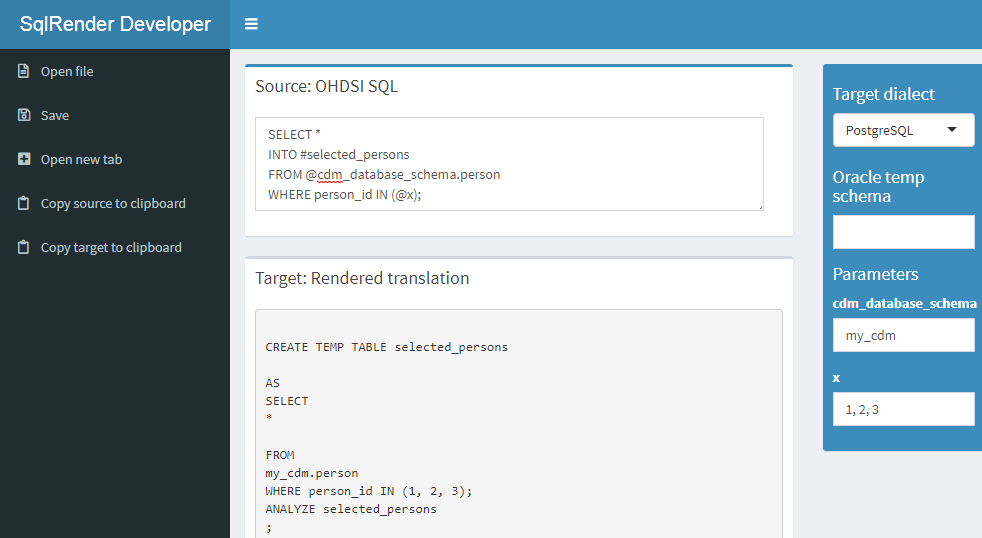
\includegraphics[width=1\linewidth]{images/SqlAndR/sqlDeveloper} 

}

\caption{The SqlDeveloper Shiny app.}\label{fig:sqlDeveloper}
\end{figure}

In the app you can enter OHDSI SQL, select the target dialect as well as
provide values for the parameters that appear in your SQL, and the
translation will automatically appear at the bottom.

\section{DatabaseConnector}\label{DatabaseConnector}

\href{https://ohdsi.github.io/DatabaseConnector/}{DatabaseConnector} is
an R package for connecting to various database platforms using Java's
JDBC drivers. The DatabaseConnector package is available on CRAN (the
Comprehensive R Archive Network), and can therefore be installed using:

\begin{Shaded}
\begin{Highlighting}[]
\KeywordTok{install.packages}\NormalTok{(}\StringTok{"DatabaseConnector"}\NormalTok{)}
\end{Highlighting}
\end{Shaded}

DatabaseConnector supports a wide array of technical platforms including
traditional database systems (PostgreSQL, Microsoft SQL Server, SQLite,
and Oracle), parallel data warehouses (Microsoft APS, IBM Netezza, and
Amazon RedShift), as well as Big Data platforms (Hadoop through Impala,
and Google BigQuery). The package already contains most drivers, but
because of licensing reasons the drivers for BigQuery, Netezza and
Impala are not included but must be obtained by the user. Type
\texttt{?jdbcDrivers} for instructions on how to download these drivers.
Once downloaded, you can use the \texttt{pathToDriver} argument of the
\texttt{connect}, \texttt{dbConnect}, and
\texttt{createConnectionDetails} functions.

\subsection{Creating a connection}\label{creating-a-connection}

To connect to a database a number of details need to be specified, such
as the database platform, the location of the server, the user name, and
password. We can call the \texttt{connect} function and specify these
details directly:

\begin{Shaded}
\begin{Highlighting}[]
\NormalTok{conn <-}\StringTok{ }\KeywordTok{connect}\NormalTok{(}\DataTypeTok{dbms =} \StringTok{"postgresql"}\NormalTok{,}
                \DataTypeTok{server =} \StringTok{"localhost/postgres"}\NormalTok{,}
                \DataTypeTok{user =} \StringTok{"joe"}\NormalTok{,}
                \DataTypeTok{password =} \StringTok{"secret"}\NormalTok{,}
                \DataTypeTok{schema =} \StringTok{"cdm"}\NormalTok{)}
\end{Highlighting}
\end{Shaded}

\begin{verbatim}
## Connecting using PostgreSQL driver
\end{verbatim}

See \texttt{?connect} for information on which details are required for
each platform. Don't forget to close any connection afterwards:

\begin{Shaded}
\begin{Highlighting}[]
\KeywordTok{disconnect}\NormalTok{(conn)}
\end{Highlighting}
\end{Shaded}

Note that, instead of providing the server name, it is also possible to
provide the JDBC connection string if this is more convenient:

\begin{Shaded}
\begin{Highlighting}[]
\NormalTok{connString <-}\StringTok{ "jdbc:postgresql://localhost:5432/postgres"}
\NormalTok{conn <-}\StringTok{ }\KeywordTok{connect}\NormalTok{(}\DataTypeTok{dbms =} \StringTok{"postgresql"}\NormalTok{,}
                \DataTypeTok{connectionString =}\NormalTok{ connString,}
                \DataTypeTok{user =} \StringTok{"joe"}\NormalTok{,}
                \DataTypeTok{password =} \StringTok{"secret"}\NormalTok{,}
                \DataTypeTok{schema =} \StringTok{"cdm"}\NormalTok{)}
\end{Highlighting}
\end{Shaded}

\begin{verbatim}
## Connecting using PostgreSQL driver
\end{verbatim}

Sometimes we may want to first specify the connection details, and defer
connecting until later. This may be convenient for example when the
connection is established inside a function, and the details need to be
passed as an argument. We can use the \texttt{createConnectionDetails}
function for this purpose:

\begin{Shaded}
\begin{Highlighting}[]
\NormalTok{details <-}\StringTok{ }\KeywordTok{createConnectionDetails}\NormalTok{(}\DataTypeTok{dbms =} \StringTok{"postgresql"}\NormalTok{,}
                                   \DataTypeTok{server =} \StringTok{"localhost/postgres"}\NormalTok{,}
                                   \DataTypeTok{user =} \StringTok{"joe"}\NormalTok{,}
                                   \DataTypeTok{password =} \StringTok{"secret"}\NormalTok{,}
                                   \DataTypeTok{schema =} \StringTok{"cdm"}\NormalTok{)}
\NormalTok{conn <-}\StringTok{ }\KeywordTok{connect}\NormalTok{(details)}
\end{Highlighting}
\end{Shaded}

\begin{verbatim}
## Connecting using PostgreSQL driver
\end{verbatim}

\subsection{Querying}\label{querying}

The main functions for querying database are the \texttt{querySql} and
\texttt{executeSql} functions. The difference between these functions is
that \texttt{querySql} expects data to be returned by the database, and
can handle only one SQL statement at a time. In contrast,
\texttt{executeSql} does not expect data to be returned, and accepts
multiple SQL statements in a single SQL string.

Some examples:

\begin{Shaded}
\begin{Highlighting}[]
\KeywordTok{querySql}\NormalTok{(conn, }\StringTok{"SELECT TOP 3 * FROM person"}\NormalTok{)}
\end{Highlighting}
\end{Shaded}

\begin{verbatim}
##   PERSON_ID GENDER_CONCEPT_ID YEAR_OF_BIRTH
## 1         1              8507          1975
## 2         2              8507          1976
## 3         3              8507          1977
\end{verbatim}

\begin{Shaded}
\begin{Highlighting}[]
\KeywordTok{executeSql}\NormalTok{(conn, }\StringTok{"TRUNCATE TABLE foo; DROP TABLE foo;"}\NormalTok{)}
\end{Highlighting}
\end{Shaded}

Both function provide extensive error reporting: When an error is thrown
by the server, the error message and the offending piece of SQL are
written to a text file to allow better debugging. The
\texttt{executeSql} function also by default shows a progress bar,
indicating the percentage of SQL statements that has been executed. If
those attributes are not desired, the package also offers the
\texttt{lowLevelQuerySql} and \texttt{lowLevelExecuteSql} functions.

\subsection{Querying using ffdf
objects}\label{querying-using-ffdf-objects}

Sometimes the data to be fetched from the database is too large to fit
into memory. As mentioned in Section \ref{BigDataSupport}, in such a
case we can use the \texttt{ff} package to store R data objects on file,
and use them as if they are available in memory.
\texttt{DatabaseConnector} can download data directly into ffdf objects:

\begin{Shaded}
\begin{Highlighting}[]
\NormalTok{x <-}\StringTok{ }\KeywordTok{querySql.ffdf}\NormalTok{(conn, }\StringTok{"SELECT * FROM person"}\NormalTok{)}
\end{Highlighting}
\end{Shaded}

Where x is now an ffdf object.

\subsection{Querying different platforms using the same
SQL}\label{querying-different-platforms-using-the-same-sql}

The following convenience functions are available that first call the
\texttt{render} and \texttt{translate} functions in the SqlRender
package: \texttt{renderTranslateExecuteSql},
\texttt{renderTranslateQuerySql}, \texttt{renderTranslateQuerySql.ffdf}.
For example:

\begin{Shaded}
\begin{Highlighting}[]
\NormalTok{x <-}\StringTok{ }\KeywordTok{renderTranslateQuerySql}\NormalTok{(conn, }
                             \DataTypeTok{sql =} \StringTok{"SELECT TOP 10 * FROM @schema.person"}\NormalTok{,}
                             \DataTypeTok{schema =} \StringTok{"cdm_synpuf"}\NormalTok{)}
\end{Highlighting}
\end{Shaded}

Note that the SQL Server-specific `TOP 10' syntax will be translated to
for example `LIMIT 10' on PostgreSQL, and that the SQL parameter
\texttt{@schema} will be instantiated with the provided value
`cdm\_synpuf'.

\subsection{Inserting tables}\label{inserting-tables}

Although it is also possible to insert data in the database by sending
SQL statements using the \texttt{executeSql} function, it is often more
convenient and faster (due to some optimization) to use the
\texttt{insertTable} function:

\begin{Shaded}
\begin{Highlighting}[]
\KeywordTok{data}\NormalTok{(mtcars)}
\KeywordTok{insertTable}\NormalTok{(conn, }\StringTok{"mtcars"}\NormalTok{, mtcars, }\DataTypeTok{createTable =} \OtherTok{TRUE}\NormalTok{)}
\end{Highlighting}
\end{Shaded}

In this example, we're uploading the mtcars data frame to a table called
`mtcars' on the server, which will be automatically created.

\section{Querying the CDM}\label{QueryTheCdm}

In the following examples we use OHDSI SQL to query a database that
adheres to the CDM. These queries use \texttt{@cdm} to denote the
database schema where the data in CDM can be found.

We can start by just querying how many people are in the database:

\begin{Shaded}
\begin{Highlighting}[]
\KeywordTok{SELECT} \FunctionTok{COUNT}\NormalTok{(*) }\KeywordTok{AS}\NormalTok{ person_count }\KeywordTok{FROM}\NormalTok{ @cdm.person;}
\end{Highlighting}
\end{Shaded}

\begin{longtable}[]{@{}r@{}}
\toprule
PERSON\_COUNT\tabularnewline
\midrule
\endhead
26299001\tabularnewline
\bottomrule
\end{longtable}

Or perhaps we're interested in the average length of an observation
period:

\begin{Shaded}
\begin{Highlighting}[]
\KeywordTok{SELECT} \FunctionTok{AVG}\NormalTok{(DATEDIFF(}\DataTypeTok{DAY}\NormalTok{, }
\NormalTok{                    observation_period_start_date, }
\NormalTok{                    observation_period_end_date) / }\FloatTok{365.25}\NormalTok{) }\KeywordTok{AS}\NormalTok{ num_years}
\KeywordTok{FROM}\NormalTok{ @cdm.observation_period;}
\end{Highlighting}
\end{Shaded}

\begin{longtable}[]{@{}r@{}}
\toprule
NUM\_YEARS\tabularnewline
\midrule
\endhead
1.980803\tabularnewline
\bottomrule
\end{longtable}

We can join tables to produce additional statistics. A join combines
fields from multiple tables, typically by requiring specific fields in
the tables to have the same value. For example, here we join the PERSON
table to the OBSERVATION\_PERIOD table on the person\_id fields in both
tables. In other words, the result of the join is a new table-like set
that has all the fields of the two tables, but in all rows the
person\_id fields from the two tables must have the same value. We can
now for example compute the maximum age at observation end by using the
observation\_period\_end\_date field from the OBSERVATION\_PERIOD table
together with the year\_of\_birth field of the PERSON table:

\begin{Shaded}
\begin{Highlighting}[]
\KeywordTok{SELECT} \FunctionTok{MAX}\NormalTok{(}\DataTypeTok{YEAR}\NormalTok{(observation_period_end_date) -}
\NormalTok{           year_of_birth) }\KeywordTok{AS}\NormalTok{ max_age}
\KeywordTok{FROM}\NormalTok{ @cdm.person}
\KeywordTok{INNER} \KeywordTok{JOIN}\NormalTok{ @cdm.observation_period}
  \KeywordTok{ON}\NormalTok{ person.person_id = observation_period.person_id;}
\end{Highlighting}
\end{Shaded}

\begin{longtable}[]{@{}r@{}}
\toprule
MAX\_AGE\tabularnewline
\midrule
\endhead
90\tabularnewline
\bottomrule
\end{longtable}

A much more complicated query is needed to determine the distribution of
age at the start of observation. In this query, we first join the PERSON
to the OBSERVATION\_PERIOD table to compute age at start of observetion.
We also compute the ordering for this joined set based on age, and store
it as order\_nr. Because we want to use the result of this join multiple
times, we define it as a common table expression (CTE) (defined using
\texttt{WITH\ ...\ AS}) that we call ``ages'', meaning We can refer to
ages as if it is an existing table. We count the number of rows in ages
to produce ``n'', and then for each quantile find the minimum age where
the order\_nr is smaller than the fraction times n. For example, median
we use the minimum age where \(order\_nr < .50 * n\). The minimum and
maximum age are computed separately:

\begin{Shaded}
\begin{Highlighting}[]
\KeywordTok{WITH}\NormalTok{ ages}
\KeywordTok{AS}\NormalTok{ (}
    \KeywordTok{SELECT}\NormalTok{ age,}
        \FunctionTok{ROW_NUMBER}\NormalTok{() }\KeywordTok{OVER}\NormalTok{ (}
            \KeywordTok{ORDER} \KeywordTok{BY}\NormalTok{ age}
\NormalTok{            ) order_nr}
    \KeywordTok{FROM}\NormalTok{ (}
        \KeywordTok{SELECT} \DataTypeTok{YEAR}\NormalTok{(observation_period_start_date) - year_of_birth }\KeywordTok{AS}\NormalTok{ age}
        \KeywordTok{FROM}\NormalTok{ @cdm.person}
        \KeywordTok{INNER} \KeywordTok{JOIN}\NormalTok{ @cdm.observation_period}
            \KeywordTok{ON}\NormalTok{ person.person_id = observation_period.person_id}
\NormalTok{        ) age_computed}
\NormalTok{    )}
\KeywordTok{SELECT} \FunctionTok{MIN}\NormalTok{(age) }\KeywordTok{AS}\NormalTok{ min_age,}
    \FunctionTok{MIN}\NormalTok{(}\KeywordTok{CASE} 
            \KeywordTok{WHEN}\NormalTok{ order_nr < .}\DecValTok{25}\NormalTok{ * n}
                \KeywordTok{THEN} \DecValTok{9999}
            \KeywordTok{ELSE}\NormalTok{ age}
            \KeywordTok{END}\NormalTok{) }\KeywordTok{AS}\NormalTok{ q25_age,}
    \FunctionTok{MIN}\NormalTok{(}\KeywordTok{CASE} 
            \KeywordTok{WHEN}\NormalTok{ order_nr < .}\DecValTok{50}\NormalTok{ * n}
                \KeywordTok{THEN} \DecValTok{9999}
            \KeywordTok{ELSE}\NormalTok{ age}
            \KeywordTok{END}\NormalTok{) }\KeywordTok{AS}\NormalTok{ median_age,}
    \FunctionTok{MIN}\NormalTok{(}\KeywordTok{CASE} 
            \KeywordTok{WHEN}\NormalTok{ order_nr < .}\DecValTok{75}\NormalTok{ * n}
                \KeywordTok{THEN} \DecValTok{9999}
            \KeywordTok{ELSE}\NormalTok{ age}
            \KeywordTok{END}\NormalTok{) }\KeywordTok{AS}\NormalTok{ q75_age,}
    \FunctionTok{MAX}\NormalTok{(age) }\KeywordTok{AS}\NormalTok{ max_age}
\KeywordTok{FROM}\NormalTok{ ages}
\KeywordTok{CROSS} \KeywordTok{JOIN}\NormalTok{ (}
    \KeywordTok{SELECT} \FunctionTok{COUNT}\NormalTok{(*) }\KeywordTok{AS}\NormalTok{ n}
    \KeywordTok{FROM}\NormalTok{ ages}
\NormalTok{    ) population_size;}
\end{Highlighting}
\end{Shaded}

\begin{longtable}[]{@{}rrrrr@{}}
\toprule
MIN\_AGE & Q25\_AGE & MEDIAN\_AGE & Q75\_AGE & MAX\_AGE\tabularnewline
\midrule
\endhead
0 & 6 & 17 & 34 & 90\tabularnewline
\bottomrule
\end{longtable}

More complex computations can also be performed in R instead of using
SQL. For example, we can get the same answer using this R code:

\begin{Shaded}
\begin{Highlighting}[]
\NormalTok{sql <-}\StringTok{ "SELECT YEAR(observation_period_start_date) -}
\StringTok{               year_of_birth AS age}
\StringTok{FROM @cdm.person}
\StringTok{INNER JOIN @cdm.observation_period}
\StringTok{  ON person.person_id = observation_period.person_id;"}
\NormalTok{age <-}\StringTok{ }\KeywordTok{renderTranslateQuerySql}\NormalTok{(conn, sql, }\DataTypeTok{cdm =} \StringTok{"cdm"}\NormalTok{)}
\KeywordTok{quantile}\NormalTok{(age[, }\DecValTok{1}\NormalTok{], }\KeywordTok{c}\NormalTok{(}\DecValTok{0}\NormalTok{, }\FloatTok{0.25}\NormalTok{, }\FloatTok{0.5}\NormalTok{, }\FloatTok{0.75}\NormalTok{, }\DecValTok{1}\NormalTok{))}
\end{Highlighting}
\end{Shaded}

\begin{verbatim}
##   0%  25%  50%  75% 100% 
##    0    6   17   34   90
\end{verbatim}

Here we compute age on the server, download all ages, and then compute
the age distribution. However, this requires millions of rows of data to
be downloaded from the database server, and is therefore not very
efficient. You will need to decide on a case-by-case basis whether a
computation is best performed in SQL or in R.

Queries can use the source values in the CDM. For example, we can
retrieve the top 10 most frequent condition source codes using:

\begin{Shaded}
\begin{Highlighting}[]
\KeywordTok{SELECT}\NormalTok{ TOP }\DecValTok{10}\NormalTok{ condition_source_value, }
  \FunctionTok{COUNT}\NormalTok{(*) }\KeywordTok{AS}\NormalTok{ code_count}
\KeywordTok{FROM}\NormalTok{ @cdm.condition_occurrence}
\KeywordTok{GROUP} \KeywordTok{BY}\NormalTok{ condition_source_value}
\KeywordTok{ORDER} \KeywordTok{BY}\NormalTok{ -COUNT(*);}
\end{Highlighting}
\end{Shaded}

\begin{longtable}[]{@{}rr@{}}
\toprule
CONDITION\_SOURCE\_VALUE & CODE\_COUNT\tabularnewline
\midrule
\endhead
4019 & 49094668\tabularnewline
25000 & 36149139\tabularnewline
78099 & 28908399\tabularnewline
319 & 25798284\tabularnewline
31401 & 22547122\tabularnewline
317 & 22453999\tabularnewline
311 & 19626574\tabularnewline
496 & 19570098\tabularnewline
I10 & 19453451\tabularnewline
3180 & 18973883\tabularnewline
\bottomrule
\end{longtable}

Here we grouped records in the CONDITION\_OCCURRENCE table by values of
the condition\_source\_value field, and counted the number of records in
each group. We retrieve the condition\_source\_value and the count, and
reverse-order it by the count.

\section{Using the vocabulary when
querying}\label{using-the-vocabulary-when-querying}

Many operations require the vocabulary to be useful. The Vocabulary
tables are part of the CDM, and are therefore available using SQL
queries. Querying the Vocabulary is already described at length in
Chapter \ref{StandardizedVocabularies}. Here we show how queries against
the Vocabulary can be combined with queries against the CDM. Many fields
in the CDM contain concept IDs which can be resolved using the CONCEPT
table. For example, we may wish to count the number of persons in the
database stratified by gender, and it would be convenient to resolve the
GENDER\_CONCEPT\_ID field to a concept name:

\begin{Shaded}
\begin{Highlighting}[]
\KeywordTok{SELECT} \FunctionTok{COUNT}\NormalTok{(*) }\KeywordTok{AS}\NormalTok{ subject_count,}
\NormalTok{  concept_name}
\KeywordTok{FROM}\NormalTok{ @cdm.person}
\KeywordTok{INNER} \KeywordTok{JOIN}\NormalTok{ @cdm.concept}
  \KeywordTok{ON}\NormalTok{ person.gender_concept_id = concept.concept_id}
\KeywordTok{GROUP} \KeywordTok{BY}\NormalTok{ concept_name;}
\end{Highlighting}
\end{Shaded}

\begin{longtable}[]{@{}rr@{}}
\toprule
SUBJECT\_COUNT & CONCEPT\_NAME\tabularnewline
\midrule
\endhead
14927548 & FEMALE\tabularnewline
11371453 & MALE\tabularnewline
\bottomrule
\end{longtable}

A very powerful feature of the Vocabulary is its hierarchy. A very
common query looks for a specific concept \emph{and all of its
descendants}. For example, image we wish to count the number of
prescriptions containing the ingredient ibuprofen:

\begin{Shaded}
\begin{Highlighting}[]
\KeywordTok{SELECT} \FunctionTok{COUNT}\NormalTok{(*) }\KeywordTok{AS}\NormalTok{ prescription_count}
\KeywordTok{FROM}\NormalTok{ @cdm.drug_exposure}
\KeywordTok{INNER} \KeywordTok{JOIN}\NormalTok{ @cdm.concept_ancestor}
  \KeywordTok{ON}\NormalTok{ drug_concept_id = descendant_concept_id}
\KeywordTok{INNER} \KeywordTok{JOIN}\NormalTok{ @cdm.concept ingredient}
  \KeywordTok{ON}\NormalTok{ ancestor_concept_id = ingredient.concept_id}
\KeywordTok{WHERE}\NormalTok{ ingredient.concept_name = }\StringTok{'Ibuprofen'}
  \KeywordTok{AND}\NormalTok{ ingredient.concept_class_id = }\StringTok{'Ingredient'}
  \KeywordTok{AND}\NormalTok{ ingredient.standard_concept = }\StringTok{'S'}\NormalTok{;}
\end{Highlighting}
\end{Shaded}

\begin{longtable}[]{@{}r@{}}
\toprule
PRESCRIPTION\_COUNT\tabularnewline
\midrule
\endhead
26871214\tabularnewline
\bottomrule
\end{longtable}

\section{QueryLibrary}\label{querylibrary}

TODO: update this section when QueryLibrary is finalized.

QueryLibrary is a library of commonly-used SQL queries for the CDM. It
is available as an online application \footnote{\url{http:/data.ohdsi.org/QueryLibrary}}
shown in Figure \ref{fig:queryLibrary}, and as an R package\footnote{\url{https://github.com/OHDSI/QueryLibrary}}.

\begin{figure}

{\centering 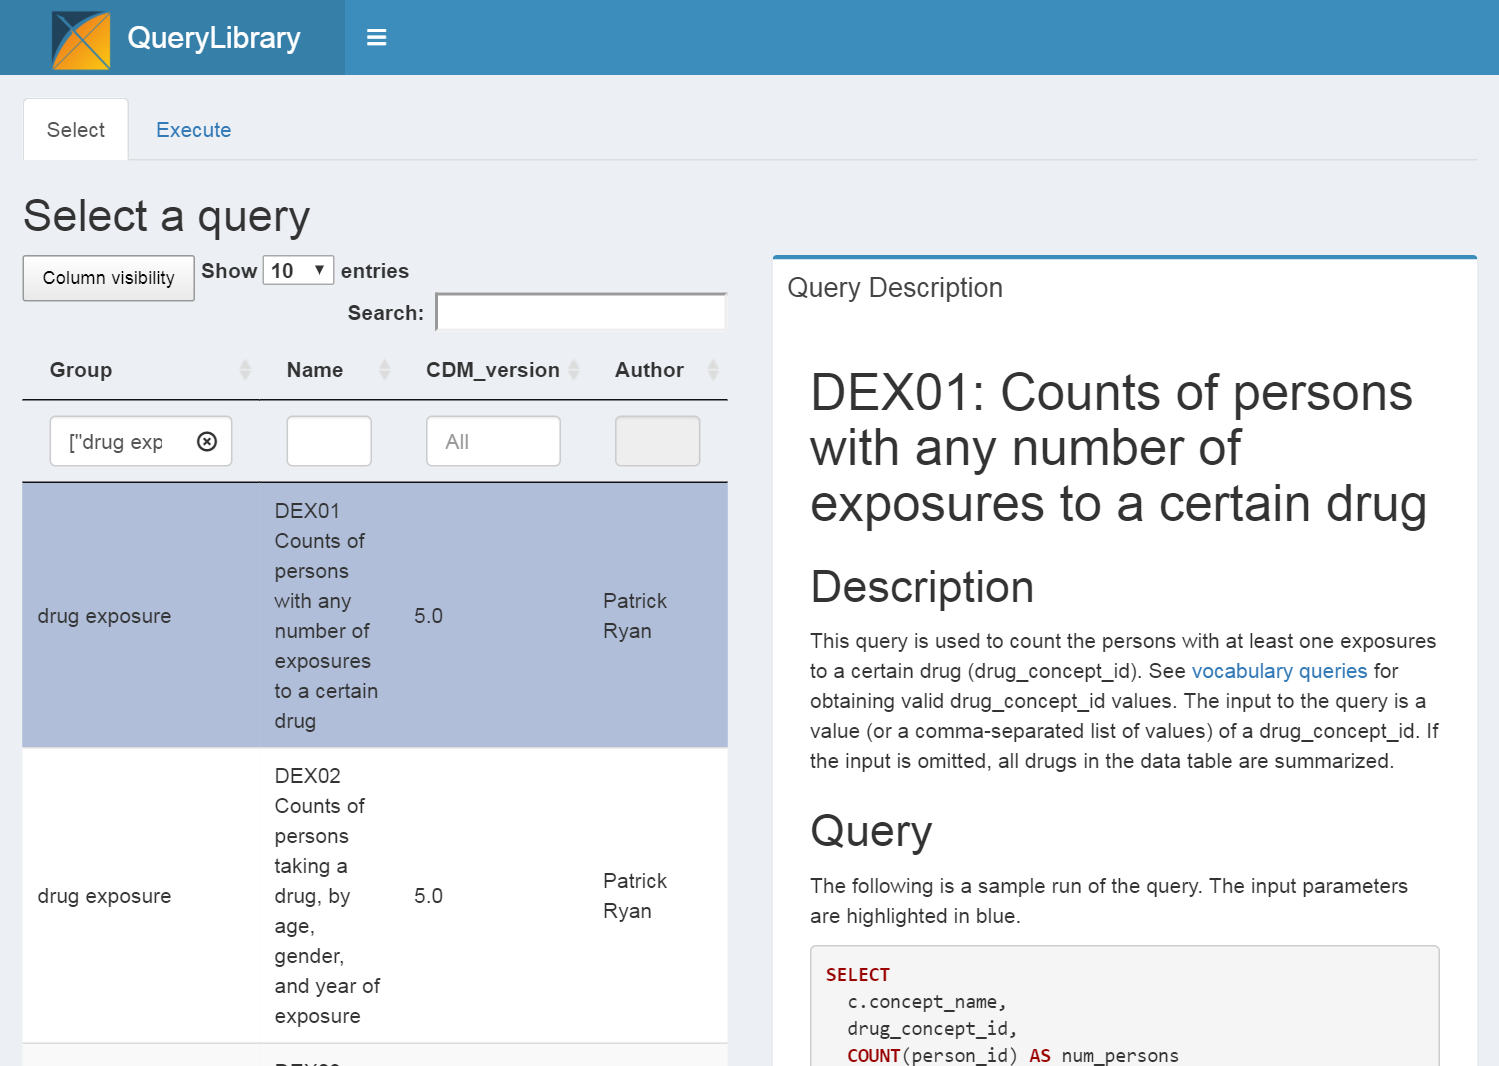
\includegraphics[width=1\linewidth]{images/SqlAndR/queryLibrary} 

}

\caption{QueryLibrary: a library of SQL queries against the CDM.}\label{fig:queryLibrary}
\end{figure}

The purpose of the library is to help new users learn how to query the
CDM. The queries in the library have been reviewed and approved by the
OHDSI community. The query library is primarily intended for training
purposes, but is also a valuable resource for experienced users.

The QueryLibrary makes use of SqlRender to output the queries in the SQL
dialect of choice. Users can also specify the CDM database schema,
vocabulary database schema (if separate), and the Oracle temp schema (if
needed), so the queries will be automatically rendered with these
settings.

\section{Designing a simple study}\label{designing-a-simple-study}

\subsection{Problem definition}\label{problem-definition}

Angioedema is a well-known side-effect of ACE inhibitors (ACEi).
\citet{slater_1988} estimate the incidence rate of angioedema in the
first week of ACEi treatment to be one case per 3,000 patients per week.
Here we seek to replicate this finding, and stratify by age and gender,
thus answering the question

\begin{quote}
What is the rate of angioedema in the first week following ACEi
treatment initiation, stratified by age and gender?
\end{quote}

\subsection{Exposure}\label{exposure}

We'll define exposure as first exposure to a drug containing an
ingredient in the ACEi class. By first we mean no earlier exposure to
any ingredient in the class. We require 365 days of continuous
observation time prior to the first exposure.

\subsection{Outcome}\label{outcome}

We define angioedema as any occurrence of an angioedema diagnose code
during an inpatient or emergency room (ER) visit.

\subsection{Time-at-risk}\label{time-at-risk}

We will compute the incidence rate in the first week following treatment
initiation, irrespective of whether patients were exposed for the full
week.

\section{Implementing the study using SQL and
R}\label{implementing-the-study-using-sql-and-r}

Although we are not bound to any of the OHDSI tool conventions, it is
helpful to follow the same principles. In this case, we will use SQL to
populate a cohort table, similarly to how the OHDSI tools work. The
COHORT table is defined in the CDM, and has a predefined set of fields
that we will also use. We first must create the COHORT table in a
database schema where we have write access, which likely is not the same
as the database schema that holds the data in CDM format.

\begin{Shaded}
\begin{Highlighting}[]
\KeywordTok{library}\NormalTok{(DatabaseConnector)}
\NormalTok{conn <-}\StringTok{ }\KeywordTok{connect}\NormalTok{(}\DataTypeTok{dbms =} \StringTok{"postgresql"}\NormalTok{,}
                \DataTypeTok{server =} \StringTok{"localhost/postgres"}\NormalTok{,}
                \DataTypeTok{user =} \StringTok{"joe"}\NormalTok{,}
                \DataTypeTok{password =} \StringTok{"secret"}\NormalTok{)}
\NormalTok{cdmDbSchema <-}\StringTok{ "cdm"}
\NormalTok{cohortDbSchema <-}\StringTok{ "scratch"}
\NormalTok{cohortTable <-}\StringTok{ "my_cohorts"}

\NormalTok{sql <-}\StringTok{ "}
\StringTok{CREATE TABLE @cohort_db_schema.@cohort_table (}
\StringTok{  cohort_definition_id INT,}
\StringTok{  cohort_start_date DATE,}
\StringTok{  cohort_end_date DATE,}
\StringTok{  subject_id BIGINT}
\StringTok{);}
\StringTok{"}
\KeywordTok{renderTranslateExecuteSql}\NormalTok{(conn, sql,}
                          \DataTypeTok{cohort_db_schema =}\NormalTok{ cohortDbSchema,}
                          \DataTypeTok{cohort_table =}\NormalTok{ cohortTable)}
\end{Highlighting}
\end{Shaded}

Here we have parameterized the database schema and table names, so we
can easily adapt them to different environments. The result is an empty
table on the database server.

\subsection{Exposure cohort}\label{exposure-cohort}

Next we create our exposure cohort, and insert it into our COHORT table:

\begin{Shaded}
\begin{Highlighting}[]
\NormalTok{sql <-}\StringTok{ "}
\StringTok{INSERT INTO @cohort_db_schema.@cohort_table (}
\StringTok{  cohort_definition_id,}
\StringTok{  cohort_start_date,}
\StringTok{  cohort_end_date,}
\StringTok{  subject_id}
\StringTok{)}
\StringTok{SELECT 1 AS cohort_definition_id,}
\StringTok{  cohort_start_date,}
\StringTok{  cohort_end_date,}
\StringTok{  subject_id}
\StringTok{FROM (}
\StringTok{  SELECT MIN(drug_exposure_start_date) AS cohort_start_date,}
\StringTok{    MIN(drug_exposure_end_date) AS cohort_end_date,}
\StringTok{    person_id AS subject_id}
\StringTok{  FROM @cdm_db_schema.drug_exposure}
\StringTok{  INNER JOIN @cdm_db_schema.concept_ancestor}
\StringTok{    ON drug_concept_id = descendant_concept_id}
\StringTok{  WHERE ancestor_concept_id IN (1335471, 1340128, 1341927,}
\StringTok{    1363749, 1308216, 1310756, 1373225, 1331235, 1334456,}
\StringTok{    1342439) -- ACE inhibitors}
\StringTok{  GROUP BY person_id}
\StringTok{) first_exposure}
\StringTok{INNER JOIN @cdm_db_schema.observation_period}
\StringTok{  ON subject_id = person_id}
\StringTok{    AND observation_period_start_date < cohort_start_date}
\StringTok{    AND observation_period_end_date > cohort_start_date}
\StringTok{WHERE DATEDIFF(DAY,}
\StringTok{               observation_period_start_date,}
\StringTok{               cohort_start_date) >= 365;}
\StringTok{"}

\KeywordTok{renderTranslateExecuteSql}\NormalTok{(conn, sql,}
                          \DataTypeTok{cohort_db_schema =}\NormalTok{ cohortDbSchema,}
                          \DataTypeTok{cohort_table =}\NormalTok{ cohortTable,}
                          \DataTypeTok{cdm_db_schema =}\NormalTok{ cdmDbSchema)}
\end{Highlighting}
\end{Shaded}

Here we use the DRUG\_EXPOSURE table, and join it the CONCEPT\_ANCESTOR
table, thus allowing us to search for the ACEi ingredients and all their
descendants, i.e.~all drugs containing an ACEi. We take the first drug
exposure per person, and then join to the OBSERVATION\_PERIOD table, and
because a person can have several observation periods we must make sure
we only join to the period containing the drug exposure. We then require
at least 365 days between the observation\_period\_start\_date and the
cohort\_start\_date.

\subsection{Outcome cohort}\label{outcome-cohort}

Finally, we must create our outcome cohort:

\begin{Shaded}
\begin{Highlighting}[]
\NormalTok{sql <-}\StringTok{ "}
\StringTok{INSERT INTO @cohort_db_schema.@cohort_table (}
\StringTok{ cohort_definition_id,}
\StringTok{ cohort_start_date,}
\StringTok{ cohort_end_date,}
\StringTok{subject_id}
\StringTok{)}
\StringTok{SELECT 2 AS cohort_definition_id,}
\StringTok{  cohort_start_date,}
\StringTok{  cohort_end_date,}
\StringTok{  subject_id}
\StringTok{FROM (}
\StringTok{  SELECT DISTINCT person_id AS subject_id,}
\StringTok{    condition_start_date AS cohort_start_date,}
\StringTok{    condition_end_date AS cohort_end_date}
\StringTok{  FROM @cdm_db_schema.condition_occurrence}
\StringTok{  INNER JOIN @cdm_db_schema.concept_ancestor}
\StringTok{    ON condition_concept_id = descendant_concept_id}
\StringTok{  WHERE ancestor_concept_id = 432791 -- Angioedema}
\StringTok{) distinct_occurrence}
\StringTok{INNER JOIN @cdm_db_schema.visit_occurrence}
\StringTok{  ON subject_id = person_id}
\StringTok{  AND visit_start_date <= cohort_start_date}
\StringTok{  AND visit_end_date >= cohort_start_date}
\StringTok{WHERE visit_concept_id IN (262, 9203,}
\StringTok{    9201) -- Inpatient or ER;}
\StringTok{"}

\KeywordTok{renderTranslateExecuteSql}\NormalTok{(conn, sql,}
                          \DataTypeTok{cohort_db_schema =}\NormalTok{ cohortDbSchema,}
                          \DataTypeTok{cohort_table =}\NormalTok{ cohortTable,}
                          \DataTypeTok{cdm_db_schema =}\NormalTok{ cdmDbSchema)}
\end{Highlighting}
\end{Shaded}

Here we join the CONDITION\_OCCURRENCE table to the CONCEPT\_ANCESTOR
table to find all occurrences of angioedema or any of its descendants.
We use DISTINCT to make sure we only select one record per day, as we
believe multiple angioedema diagnoses on the same day are more likely to
be the same occurrence rather than multiple angioedema events. We join
these occurrences to the VISIT\_OCCURRENCE table to ensure the diagnose
was made in and inpatient or ER setting.

\subsection{Incidence rate
calculation}\label{incidence-rate-calculation}

Now that our cohorts are in place, we can compute the incidence rate,
stratified by age and gender:

\begin{Shaded}
\begin{Highlighting}[]
\NormalTok{sql <-}\StringTok{ "}
\StringTok{WITH tar AS (}
\StringTok{  SELECT concept_name AS gender,}
\StringTok{    FLOOR((YEAR(cohort_start_date) -}
\StringTok{          year_of_birth) / 10) AS age,}
\StringTok{    subject_id,}
\StringTok{    cohort_start_date,}
\StringTok{    CASE WHEN DATEADD(DAY, 7, cohort_start_date) >}
\StringTok{      observation_period_end_date}
\StringTok{    THEN observation_period_end_date}
\StringTok{    ELSE DATEADD(DAY, 7, cohort_start_date)}
\StringTok{    END AS cohort_end_date}
\StringTok{  FROM @cohort_db_schema.@cohort_table}
\StringTok{  INNER JOIN @cdm_db_schema.observation_period}
\StringTok{    ON subject_id = observation_period.person_id}
\StringTok{      AND observation_period_start_date < cohort_start_date}
\StringTok{      AND observation_period_end_date > cohort_start_date}
\StringTok{  INNER JOIN @cdm_db_schema.person}
\StringTok{    ON subject_id = person.person_id}
\StringTok{  INNER JOIN @cdm_db_schema.concept}
\StringTok{    ON gender_concept_id = concept_id}
\StringTok{  WHERE cohort_definition_id = 1 -- Exposure}
\StringTok{)}
\StringTok{SELECT days.gender,}
\StringTok{    days.age,}
\StringTok{    days,}
\StringTok{    CASE WHEN events IS NULL THEN 0 ELSE events END AS events}
\StringTok{FROM (}
\StringTok{  SELECT gender,}
\StringTok{    age,}
\StringTok{    SUM(DATEDIFF(DAY, cohort_start_date,}
\StringTok{      cohort_end_date)) AS days}
\StringTok{  FROM tar}
\StringTok{  GROUP BY gender,}
\StringTok{    age}
\StringTok{) days}
\StringTok{LEFT JOIN (}
\StringTok{  SELECT gender,}
\StringTok{      age,}
\StringTok{      COUNT(*) AS events}
\StringTok{  FROM tar}
\StringTok{  INNER JOIN @cohort_db_schema.@cohort_table angioedema}
\StringTok{    ON tar.subject_id = angioedema.subject_id}
\StringTok{      AND tar.cohort_start_date <= angioedema.cohort_start_date}
\StringTok{      AND tar.cohort_end_date >= angioedema.cohort_start_date}
\StringTok{  WHERE cohort_definition_id = 2 -- Outcome}
\StringTok{  GROUP BY gender,}
\StringTok{    age}
\StringTok{) events}
\StringTok{ON days.gender = events.gender}
\StringTok{  AND days.age = events.age;}
\StringTok{"}

\NormalTok{results <-}\StringTok{ }\KeywordTok{renderTranslateQuerySql}\NormalTok{(conn, sql,}
                                   \DataTypeTok{cohort_db_schema =}\NormalTok{ cohortDbSchema,}
                                   \DataTypeTok{cohort_table =}\NormalTok{ cohortTable,}
                                   \DataTypeTok{cdm_db_schema =}\NormalTok{ cdmDbSchema,}
                                   \DataTypeTok{snakeCaseToCamelCase =} \OtherTok{TRUE}\NormalTok{)}
\end{Highlighting}
\end{Shaded}

We first create ``tar'', a CTE that contains all exposures with the
appropriate time-at-risk. Note that we truncate the time-at-risk at the
observation\_period\_end\_date. We also compute the age in 10-year bins,
and identify the gender. The advantage of using a CTE is that we can use
the same set of intermediate results several times in a query. In this
case we use it to count the total amount of time-at-risk, as well as the
number of angioedema events that occur during the time-at-risk.

We use \texttt{snakeCaseToCamelCase\ =\ TRUE} because in SQL we tend to
use snake\_case for field names (because SQL in case-insensitive),
whereas in R we tend to use camelCase (because R is case-sensitive). The
\texttt{results} data frame column names will now be in camelCase.

With the help of the ggplot2 package we can easily plot our results:

\begin{Shaded}
\begin{Highlighting}[]
\CommentTok{# Compute incidence rate (IR) :}
\NormalTok{results}\OperatorTok{$}\NormalTok{ir <-}\StringTok{ }\DecValTok{1000} \OperatorTok{*}\StringTok{ }\NormalTok{results}\OperatorTok{$}\NormalTok{events }\OperatorTok{/}\StringTok{ }\NormalTok{results}\OperatorTok{$}\NormalTok{days }\OperatorTok{/}\StringTok{ }\DecValTok{7}

\CommentTok{# Fix age scale:}
\NormalTok{results}\OperatorTok{$}\NormalTok{age <-}\StringTok{ }\NormalTok{results}\OperatorTok{$}\NormalTok{age }\OperatorTok{*}\StringTok{ }\DecValTok{10}

\KeywordTok{library}\NormalTok{(ggplot2)}
\KeywordTok{ggplot}\NormalTok{(results, }\KeywordTok{aes}\NormalTok{(}\DataTypeTok{x =}\NormalTok{ age, }\DataTypeTok{y =}\NormalTok{ ir, }\DataTypeTok{group =}\NormalTok{ gender, }\DataTypeTok{color =}\NormalTok{ gender)) }\OperatorTok{+}
\StringTok{  }\KeywordTok{geom_line}\NormalTok{() }\OperatorTok{+}
\StringTok{  }\KeywordTok{xlab}\NormalTok{(}\StringTok{"Age"}\NormalTok{) }\OperatorTok{+}
\StringTok{  }\KeywordTok{ylab}\NormalTok{(}\StringTok{"Incidence (per 1,000 patient weeks)"}\NormalTok{)}
\end{Highlighting}
\end{Shaded}

\begin{center}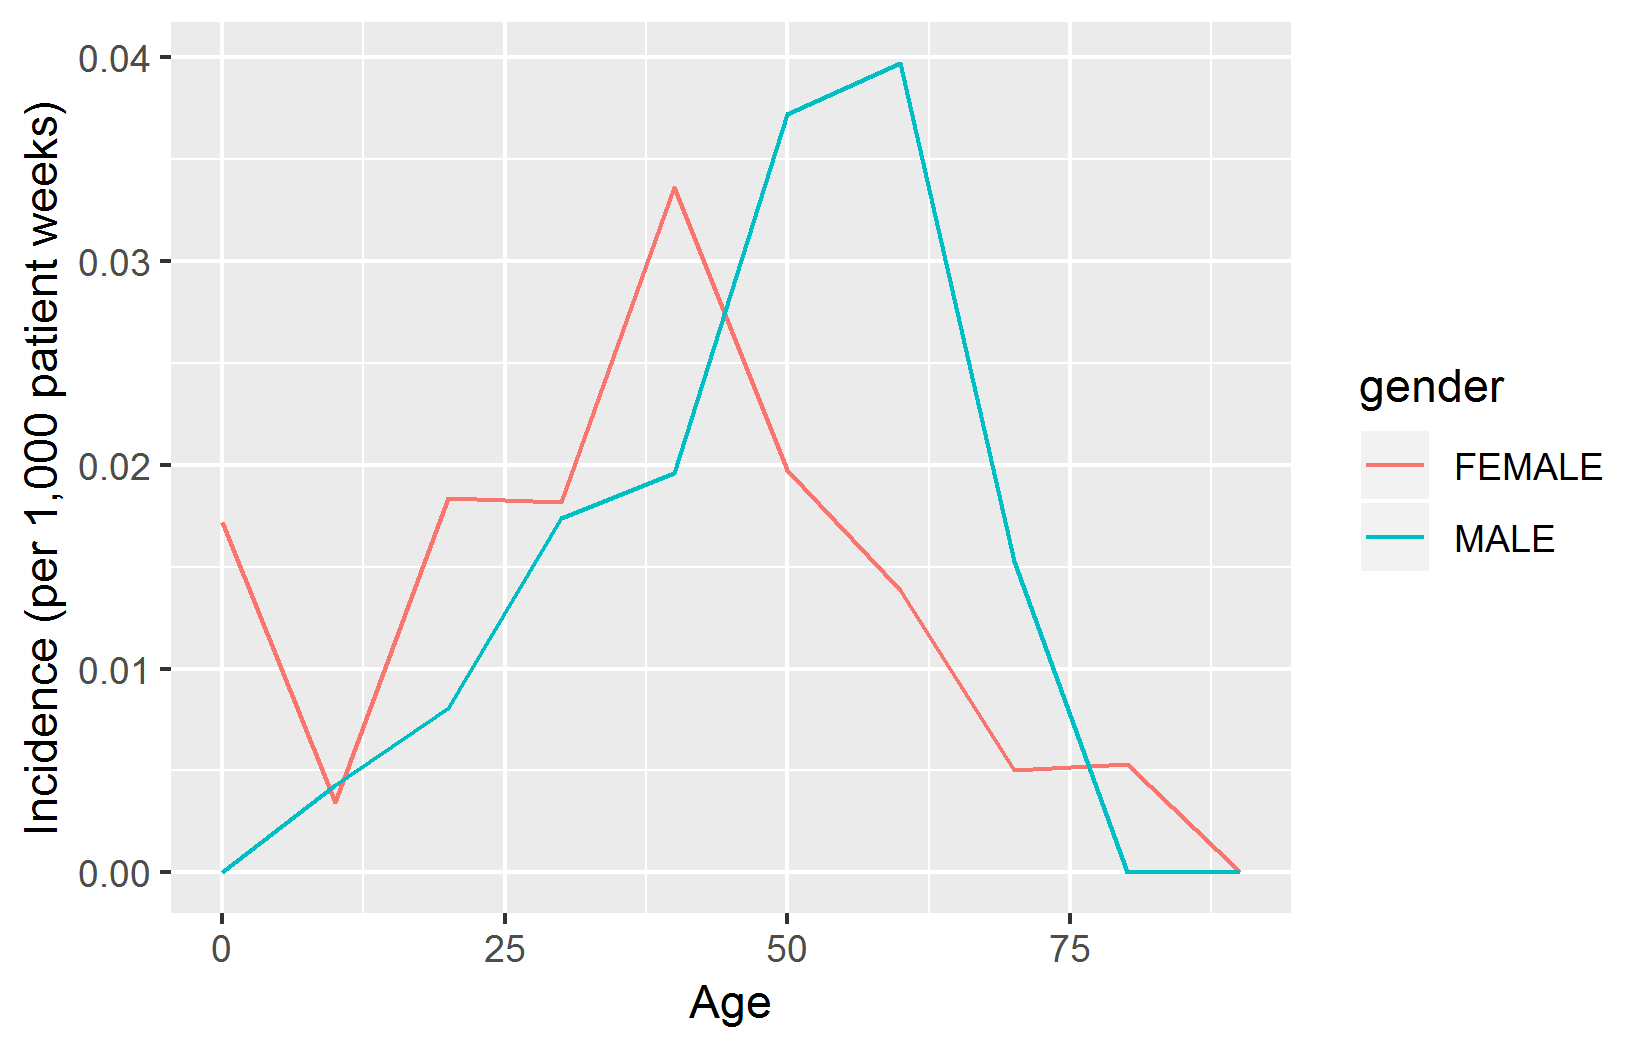
\includegraphics[width=0.8\linewidth]{images/SqlAndR/ir} \end{center}

\subsection{Clean up}\label{clean-up}

Don't forget to clean up the table we created, and to close the
connection:

\begin{Shaded}
\begin{Highlighting}[]
\NormalTok{sql <-}\StringTok{ "}
\StringTok{TRUNCATE TABLE @cohort_db_schema.@cohort_table;}
\StringTok{DROP TABLE @cohort_db_schema.@cohort_table;}
\StringTok{"}
\KeywordTok{renderTranslateExecuteSql}\NormalTok{(conn, sql,}
                          \DataTypeTok{cohort_db_schema =}\NormalTok{ cohortDbSchema,}
                          \DataTypeTok{cohort_table =}\NormalTok{ cohortTable)}

\KeywordTok{disconnect}\NormalTok{(conn)}
\end{Highlighting}
\end{Shaded}

\subsection{Compatibility}\label{compatibility}

Because we use OHDSI SQL together with DatabaseConnector and SqlRender
throughout, the code we reviewed here will run on any database platform
supported by OHDSI.

Note that for demonstration purposes we chose to create our cohorts
using hand-crafted SQL. It would probably have been more convenient to
construct cohort definition in ATLAS, and use the SQL generated by ATLAS
to instantiate the cohorts. ATLAS also produced OHDSI SQL, and can
therefore easily be used together with SqlRender and DatabaseConnector.

\section{Summary}\label{summary-2}

\BeginKnitrBlock{rmdsummary}
\begin{itemize}
\item
  \textbf{SQL} (Structured Query Language) is a standard language for
  querying databases, including those that conform to the Common Data
  Model (CDM).
\item
  Different database platforms have different SQL dialects, and require
  different tools to query them.
\item
  The \textbf{SqlRender} and \textbf{DatabaseConnector} R packages
  provide a unified way to query data in the CDM, allowing the same
  analysis code to be run in different environments without
  modificiation.
\item
  By using R and SQL together we can implement custom analyses that are
  not supported by the OHDSI tools.
\item
  The \textbf{QueryLibrary} provides a collection of re-usable SQL
  queries for the CDM.
\end{itemize}
\EndKnitrBlock{rmdsummary}

\section{Exercises}\label{exercises-1}

\chapter{Building the building blocks: cohorts}\label{Cohorts}

Introduction: a cohort is a group of people that meet a set of criteria
for a particular span of time etc. Cohorts are used throughout OHDSIs
analytical tools as the primary building blocks.

Using ATLAS: use material from Patrick's tutorial on cohort building

Using SQL: For advanced users, explain how cohorts can be created
programmatically.

Probabilistic cohorts: Aphrodite?

Case study: some example cohort definitions

\chapter{Characterization}\label{Characterization}

ATLAS' incidence rate calculator + cohort characterization tool

FeatureExtraction package:
\url{https://github.com/OHDSI/FeatureExtraction}

Case study: characteristics + IRs of some cohorts

Example .. \url{http://www.pnas.org/content/113/27/7329}

\chapter{Population-level estimation}\label{PopulationLevelEstimation}

\emph{Chapter leads: Martijn Schuemie, David Madigan, Marc Suchard \&
Patrick Ryan}

Observational healthcare data, such as administrative claims and
electronic health records, offer opportunities to generate real-world
evidence about the effect of treatments that can meaningfully improve
the lives of patients. In this chapter we focus on population-level
effect estimation, that is, the estimation of average causal effects of
exposures (e.g.~medical interventions such as drug exposures or
procedures) on specific health outcomes of interest. In what follows, we
consider two different estimation tasks:

\begin{itemize}
\tightlist
\item
  \textbf{Direct effect estimation}: estimating the effect of an
  exposure on the risk of an outcome, as compared to no exposure.
\item
  \textbf{Comparative effect estimation}: estimating the effect of an
  exposure (the target exposure) on the risk of an outcome, as compared
  to another exposure (the comparator exposure).
\end{itemize}

In both cases, the patient-level causal effect contrasts a factual
outcome, i.e., what happened to the exposed patient, with a
counterfactual outcome, i.e., what would have happened had the exposure
not occurred (direct) or had a different exposure occurred
(comparative). Since any one patient reveals only the factual outcome
(the fundamental problem of causal inference), the various effect
estimation designs employ different analytic devices to shed light on
the counterfactual outcomes.

Use-cases for population-level effect estimation include treatment
selection, safety surveillance, and comparative effectiveness. Methods
can test specific hypotheses one-at-a-time (e.g. `signal evaluation') or
explore multiple-hypotheses-at-once (e.g. `signal detection'). In all
cases, the objective remains the same: to produce a high-quality
estimate of the causal effect.

In this chapter we first describe various population-level estimation
study designs, all of which are implemented as R packages in the
\href{https://ohdsi.github.io/MethodsLibrary/}{OHDSI Methods Library}.
We then detail the design of an example estimation study, followed by
step-by-step guides of how to implement the design using ATLAS and R.
Finally, we review the various outputs generated by the study, including
study diagnostics and effect size estimates.

\section{The cohort method design}\label{CohortMethod}

\begin{figure}

{\centering 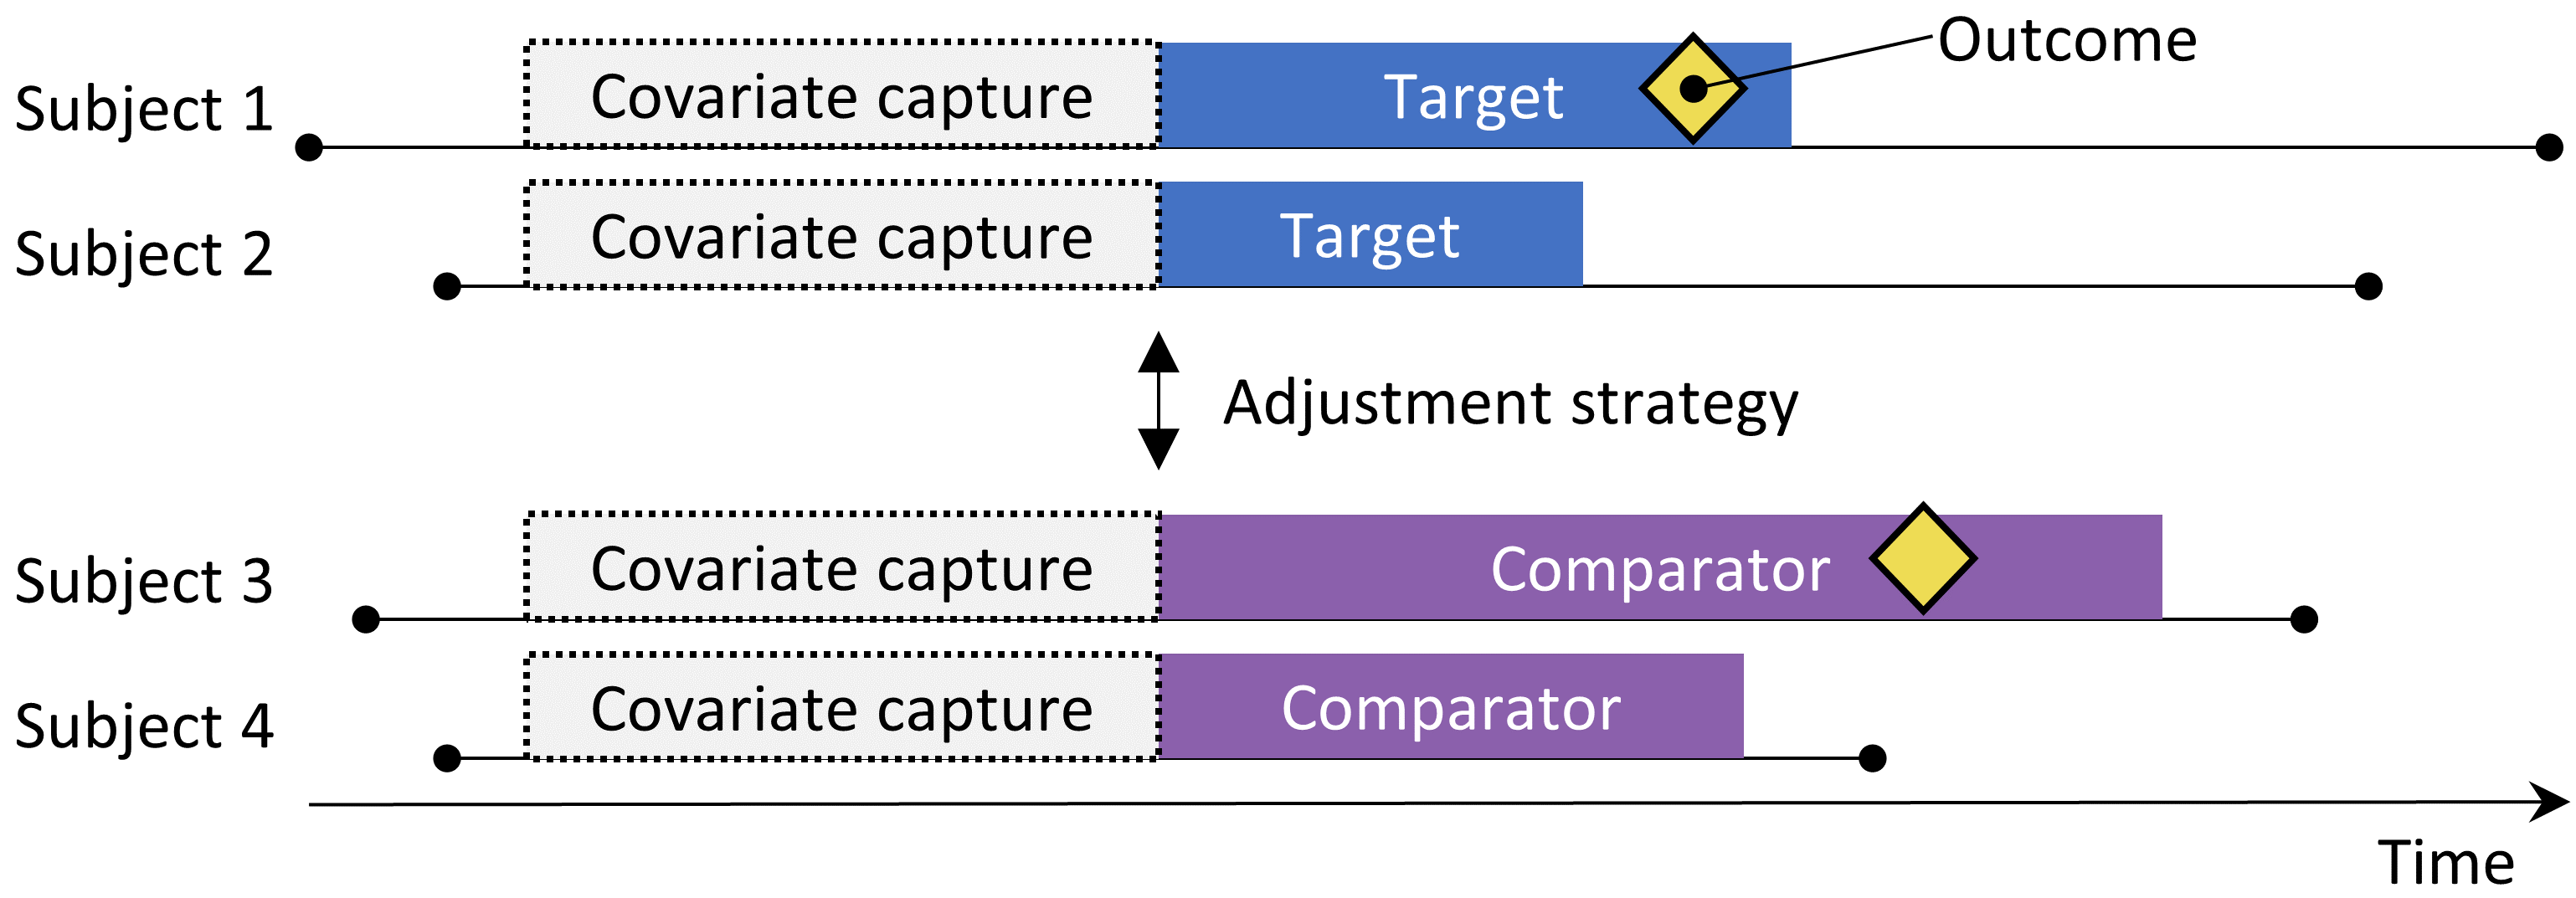
\includegraphics[width=0.9\linewidth]{images/PopulationLevelEstimation/cohortMethod} 

}

\caption{The new-user cohort design. Subjects observed to initiate the target treatment are compared to those initiating the comparator treatment. To adjust for differences between the two treatment groups several adjustment strategies can be used, such as stratification, matching, or weighting by the propensity score, or by adding baseline characateristcs to the outcome model. The chararacteristics included in the propensity model or outcome model are captured prior to treatment initiation.}\label{fig:cohortMethod}
\end{figure}

The cohort method attempts to emulate a randomized clinical trial
\citep{hernan_2016}. Subjects that are observed to initiate one
treatment (the target) are compared to subjects initiating another
treatment (the comparator) and are followed for a specific amount of
time following treatment initiation, for example the time they stay on
the treatment. We can specify the questions we wish to answer in a
cohort study by making the five choices highlighted in Table
\ref{tab:cmChoices}.

\begin{longtable}[]{@{}ll@{}}
\caption{\label{tab:cmChoices} Main design choices in a comparative cohort
design.}\tabularnewline
\toprule
\begin{minipage}[b]{0.23\columnwidth}\raggedright\strut
Choice\strut
\end{minipage} & \begin{minipage}[b]{0.71\columnwidth}\raggedright\strut
Description\strut
\end{minipage}\tabularnewline
\midrule
\endfirsthead
\toprule
\begin{minipage}[b]{0.23\columnwidth}\raggedright\strut
Choice\strut
\end{minipage} & \begin{minipage}[b]{0.71\columnwidth}\raggedright\strut
Description\strut
\end{minipage}\tabularnewline
\midrule
\endhead
\begin{minipage}[t]{0.23\columnwidth}\raggedright\strut
Target cohort\strut
\end{minipage} & \begin{minipage}[t]{0.71\columnwidth}\raggedright\strut
A cohort representing the target treatment\strut
\end{minipage}\tabularnewline
\begin{minipage}[t]{0.23\columnwidth}\raggedright\strut
Comparator cohort\strut
\end{minipage} & \begin{minipage}[t]{0.71\columnwidth}\raggedright\strut
A cohort representing the comparator treatment\strut
\end{minipage}\tabularnewline
\begin{minipage}[t]{0.23\columnwidth}\raggedright\strut
Outcome cohort\strut
\end{minipage} & \begin{minipage}[t]{0.71\columnwidth}\raggedright\strut
A cohort representing the outcome of interest\strut
\end{minipage}\tabularnewline
\begin{minipage}[t]{0.23\columnwidth}\raggedright\strut
Time-at-risk\strut
\end{minipage} & \begin{minipage}[t]{0.71\columnwidth}\raggedright\strut
At what time (often relative to the target and comparator cohort start
and end dates) do we consider the risk of the outcome?\strut
\end{minipage}\tabularnewline
\begin{minipage}[t]{0.23\columnwidth}\raggedright\strut
Model\strut
\end{minipage} & \begin{minipage}[t]{0.71\columnwidth}\raggedright\strut
The model used to estimate the effect while adjusting for differences
between the target and comparator\strut
\end{minipage}\tabularnewline
\bottomrule
\end{longtable}

The choice of model specifies, among others, the type of model. For
example, we could use a logistic regression, which evaluates whether or
not the outcome has occurred, and produces an odds ratio. A logistic
regression assumes the time-at-risk is of the same length for both
target and comparator, or is irrelevant. Alternatively, we could choose
a Poisson regression which estimates the incidence rate ratio, assuming
a constant incidence rate. Often a Cox regression is used which
considers time to first outcome to estimate the hazard ratio, assuming
proportional hazards between target and comparator.

\BeginKnitrBlock{rmdimportant}
The new-user cohort method inherently is a method for comparative effect
estimation, comparing one treatment to another. It is difficult to use
this method to compare a treatment against no treatment, since it is
hard to define a group of unexposed people that is comparable with the
exposed group. If one wants to use this design for direct effect
estimation, the preferred way is to select a comparator treatment for
the same indication as the exposure of interest, where the comparator
treatment is believed to have no effect on the outcome. Unfortunately,
such a comparator might not always be available.
\EndKnitrBlock{rmdimportant}

A key concern is that the patients receiving the target treatment may
systematically differ from those receiving the comparator treatment. For
example, suppose the target cohort is, on average, 60 years old, whereas
the comparator cohort is on average 40 years old. Comparing target to
comparator with respect to any age-related health outcome (e.g. stroke)
might then show substantial differences. An uninformed investigator
might reach the conclusion there is a causal association between the
target treatment and stroke as compared to the comparator. More
prosaically or commonplace, the investigator might conclude that there
exist target patients that experienced stroke that would not have done
so had they received the comparator. This conclusion could well be
entirely incorrect! Maybe those target patients disproportionately
experienced stroke simply because they are older; maybe the target
patients that experienced stroke might well have done so even if they
had received the comparator. In this context, age is a ``confounder''.

\subsection{Propensity scores}\label{propensity-scores}

In a randomized trial, a (virtual) coin toss assigns patients to their
respective groups. Thus, by design, the probability that a patient
receives the target treatment as against the comparator treatment does
not relate in any way to patient characteristics such as age. The coin
has no knowledge of the patient, and, what's more, we know with
certainty the exact probability that a patient receives the target
exposure. As a consequence, and with increasing confidence as the number
of patients in the trial increases, the two groups of patients
essentially \emph{cannot} differ systematically with respect to
\emph{any} patient characteristic. This guaranteed balance holds true
for characteristics that the trial measured (such as age) as well as
characteristics that the trial failed to measure.

For a given patient, the \emph{propensity score} (PS) is the probability
that that patient received the target treatment as against the
comparator. \citep{rosenbaum_1983} In a balanced two-arm randomized
trial, the propensity score is 0.5 for every patient. In a propensity
score-adjusted observational study, we estimate the probability of a
patient receiving the target treatment based on what we can observe in
the data on and before the time of treatment initiation (irrespective of
the treatment they actually received). This a straightforward predictive
modeling application; we fit a model (e.g.~a logistic regression) that
predicts whether a subject receives the target treatment, and use this
model to generate predicted probabilities (the PS) for each subject.
Unlike in a standard randomized trial, different patients will have
different probabilities of receiving the target treatment. The PS can be
used in several ways, for example by matching target subjects to
comparator subjects with similar PS, by stratifying the study population
based on the PS, or by weighting subjects using Inverse Probability of
Treatment Weighting (IPTW) derived from the PS. When matching we can
select just one comparator subject for each target subject, or we can
allow more than one comparator subject per target subject, a technique
know as variable-ratio matching. \citep{rassen_2012}

For example, suppose we use one-on-one PS matching, and that Jan has a
priori probability of 0.4 of receiving the target treatment and in fact
receives the target treatment. If we can find a patient (named Jun) that
also had an a priori probability of 0.4 of receiving the target
treatment but in fact received the comparator, the comparison of Jan and
Jun's outcomes is like a mini-randomized trial, at least with respect to
measured confounders. This comparison will yield an estimate of the
Jan-Jun causal contrast that is as good as the one randomization would
have produced. Estimation then proceeds as follows: for every patient
that received the target, find one or more matched patients that
received the comparator but had the same a priori probability of
receiving the target. Compare the outcome for the target patient with
the outcomes for the comparator patients within each of these matched
groups.

Propensity scoring controls for measured confounders. In fact, if
treatment assignment is ``strongly ignorable'' given measured
characteristics, propensity scoring will yield an unbiased estimate of
the causal effect. ``Strongly ignorable'' essentially means that there
are no unmeasured confounders, and that the measured confounders are
adjusted for appropriately. Unfortunately this is not a testable
assumption. See Chapter \ref{MethodValidity} for further discussion of
this issue.

\subsection{Variable selection}\label{VariableSelection}

In the past, PS were computed based on manually selected
characteristics, and although the OHDSI tools can support such
practices, we prefer using many generic characteristics
(i.e.~characteristics that are not selected based on the specific
exposures and outcomes in the study). \citep{tian_2018} These
characteristics include demographics, as well as all diagnoses, drug
exposures, measurement, and medical procedures observed prior to and on
the day of treatment initiation. A model typically involves 10,000 to
100,000 unique characteristics, which we fit using large-scale
regularized regression \citep{suchard_2013} implemented in the
\href{https://ohdsi.github.io/Cyclops/}{Cyclops} package. In essence, we
let the data appropriately weigh the characteristics.

\BeginKnitrBlock{rmdimportant}
We typically include the day of treatment initiation in the covariate
capture window because many relevant data points such as the diagnosis
leading to the treatment are recorded on that date. This does require us
to explicitly exclude the target and comparator treatment from the set
of covariates, because these are the things we are trying to predict.
\EndKnitrBlock{rmdimportant}

Some have argued that a data-driven approach to covariate selection that
does not depend on clinical expertise to specify the ``right'' causal
structure runs the risk of erroneously including so-called instrumental
variables and colliders, thus increasing variance and potentially
introducing bias. \citep{hernan_2002} However, these concerns are
unlikely to have a large impact in real-world scenarios.
\citep{schneeweiss_2018} Furthermore, in medicine the true causal
structure is rarely known, and when different researchers are asked to
identify the `right' covariates to include for a specific research
question, each researcher invariably comes up with a different list,
thus making the process irreproducible. Most importantly, our
diagnostics such as inspection of the propensity model, evaluating
balance on all covariates, and including negative controls would
identify most problems related to colliders and instrumental variables.

\subsection{Caliper}\label{caliper}

Since propensity scores fall on a continuum from 0 to 1, exact matching
is rarely possible. Instead, the matching process finds patients that
match the propensity score of a target patient(s) within some tolerance
known as a ``caliper.'' Following \citet{austin_2011}, we use a default
caliper of 0.2 standard deviations on the logit scale.

\subsection{Overlap: preference scores}\label{overlap-preference-scores}

The propensity method requires that matching patients exist! As such, a
key diagnostic shows the distribution of the propensity scores in the
two groups. To facilitate interpretation, the OHDSI tools plot a
transformation of the propensity score called the ``preference score''.
\citep{walker_2013} The preference score adjusts for the ``market
share'' of the two treatments. For example, if 10\% of patients receive
the target treatment (and 90\% receive the comparator treatment), then
patients with a preference score of 0.5 have a 10\% probability of
receiving the target treatment. Mathematically, the preference score is

\[\ln\left(\frac{F}{1-F}\right)=\ln\left(\frac{S}{1-S}\right)-\ln\left(\frac{P}{1-P}\right)\]

Where \(F\) is the preference score, \(S\) is the propensity score, and
\(P\) is the proportion of patients receiving the target treatment.

\citet{walker_2013} discuss the concept of ``empirical equipoise''. They
accept exposure pairs as emerging from empirical equipoise if at least
half of the exposures are to patients with a preference score of between
0.3 and 0.7.

\subsection{Balance}\label{balance}

Good practice always checks that the PS adjustment succeeds in creating
balanced groups of patients. Figure \ref{fig:balance} shows the standard
OHDSI output for checking balance. For each patient characteristic, this
plots the standardized difference between means between the two exposure
groups before and after PS adjustment. Some guidelines recommend an
after-adjustment standardized difference upper bound of 0.1.
\citep{rubin_2001}

\section{The self-controlled cohort
design}\label{the-self-controlled-cohort-design}

\begin{figure}

{\centering 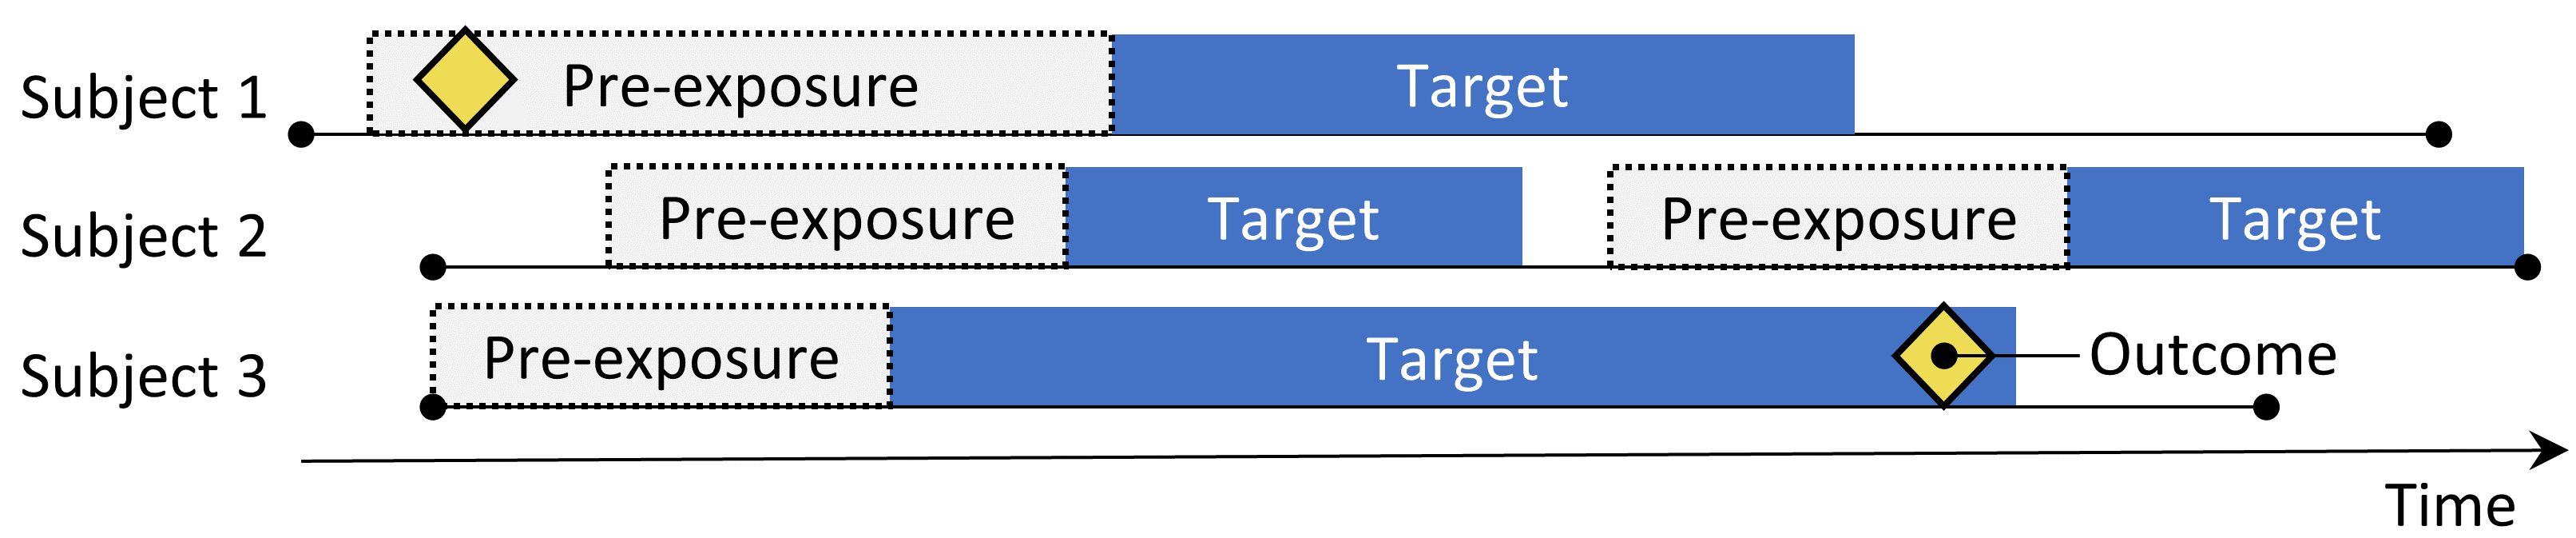
\includegraphics[width=0.9\linewidth]{images/PopulationLevelEstimation/selfControlledCohort} 

}

\caption{The self-controlled cohort design. The rate of outcomes during exposure to the target is compared to the rate of outcomes in the time pre-exposure.}\label{fig:scc}
\end{figure}

The self-controlled cohort (SCC) design \citep{ryan_2013} compares the
rate of outcomes during exposure to the rate of outcomes in the time
just prior to the exposure. The four choices shown in Table
\ref{tab:sccChoices} define a self-controlled cohort question.

\begin{longtable}[]{@{}ll@{}}
\caption{\label{tab:sccChoices} Main design choices in a self-controlled
cohort design.}\tabularnewline
\toprule
\begin{minipage}[b]{0.23\columnwidth}\raggedright\strut
Choice\strut
\end{minipage} & \begin{minipage}[b]{0.71\columnwidth}\raggedright\strut
Description\strut
\end{minipage}\tabularnewline
\midrule
\endfirsthead
\toprule
\begin{minipage}[b]{0.23\columnwidth}\raggedright\strut
Choice\strut
\end{minipage} & \begin{minipage}[b]{0.71\columnwidth}\raggedright\strut
Description\strut
\end{minipage}\tabularnewline
\midrule
\endhead
\begin{minipage}[t]{0.23\columnwidth}\raggedright\strut
Target cohort\strut
\end{minipage} & \begin{minipage}[t]{0.71\columnwidth}\raggedright\strut
A cohort representing the treatment\strut
\end{minipage}\tabularnewline
\begin{minipage}[t]{0.23\columnwidth}\raggedright\strut
Outcome cohort\strut
\end{minipage} & \begin{minipage}[t]{0.71\columnwidth}\raggedright\strut
A cohort representing the outcome of interest\strut
\end{minipage}\tabularnewline
\begin{minipage}[t]{0.23\columnwidth}\raggedright\strut
Time-at-risk\strut
\end{minipage} & \begin{minipage}[t]{0.71\columnwidth}\raggedright\strut
At what time (often relative to the target cohort start and end dates)
do we consider the risk of the outcome?\strut
\end{minipage}\tabularnewline
\begin{minipage}[t]{0.23\columnwidth}\raggedright\strut
Control time\strut
\end{minipage} & \begin{minipage}[t]{0.71\columnwidth}\raggedright\strut
The time period used as the control time\strut
\end{minipage}\tabularnewline
\bottomrule
\end{longtable}

Because the same subject that make up the exposed group are also used as
the control group, no adjustment for between-person differences need to
be made. However, the method is vulnerable to other differences, such as
differences in the baseline risk of the outcome between different time
periods.

\section{The case-control design}\label{the-case-control-design}

\begin{figure}

{\centering 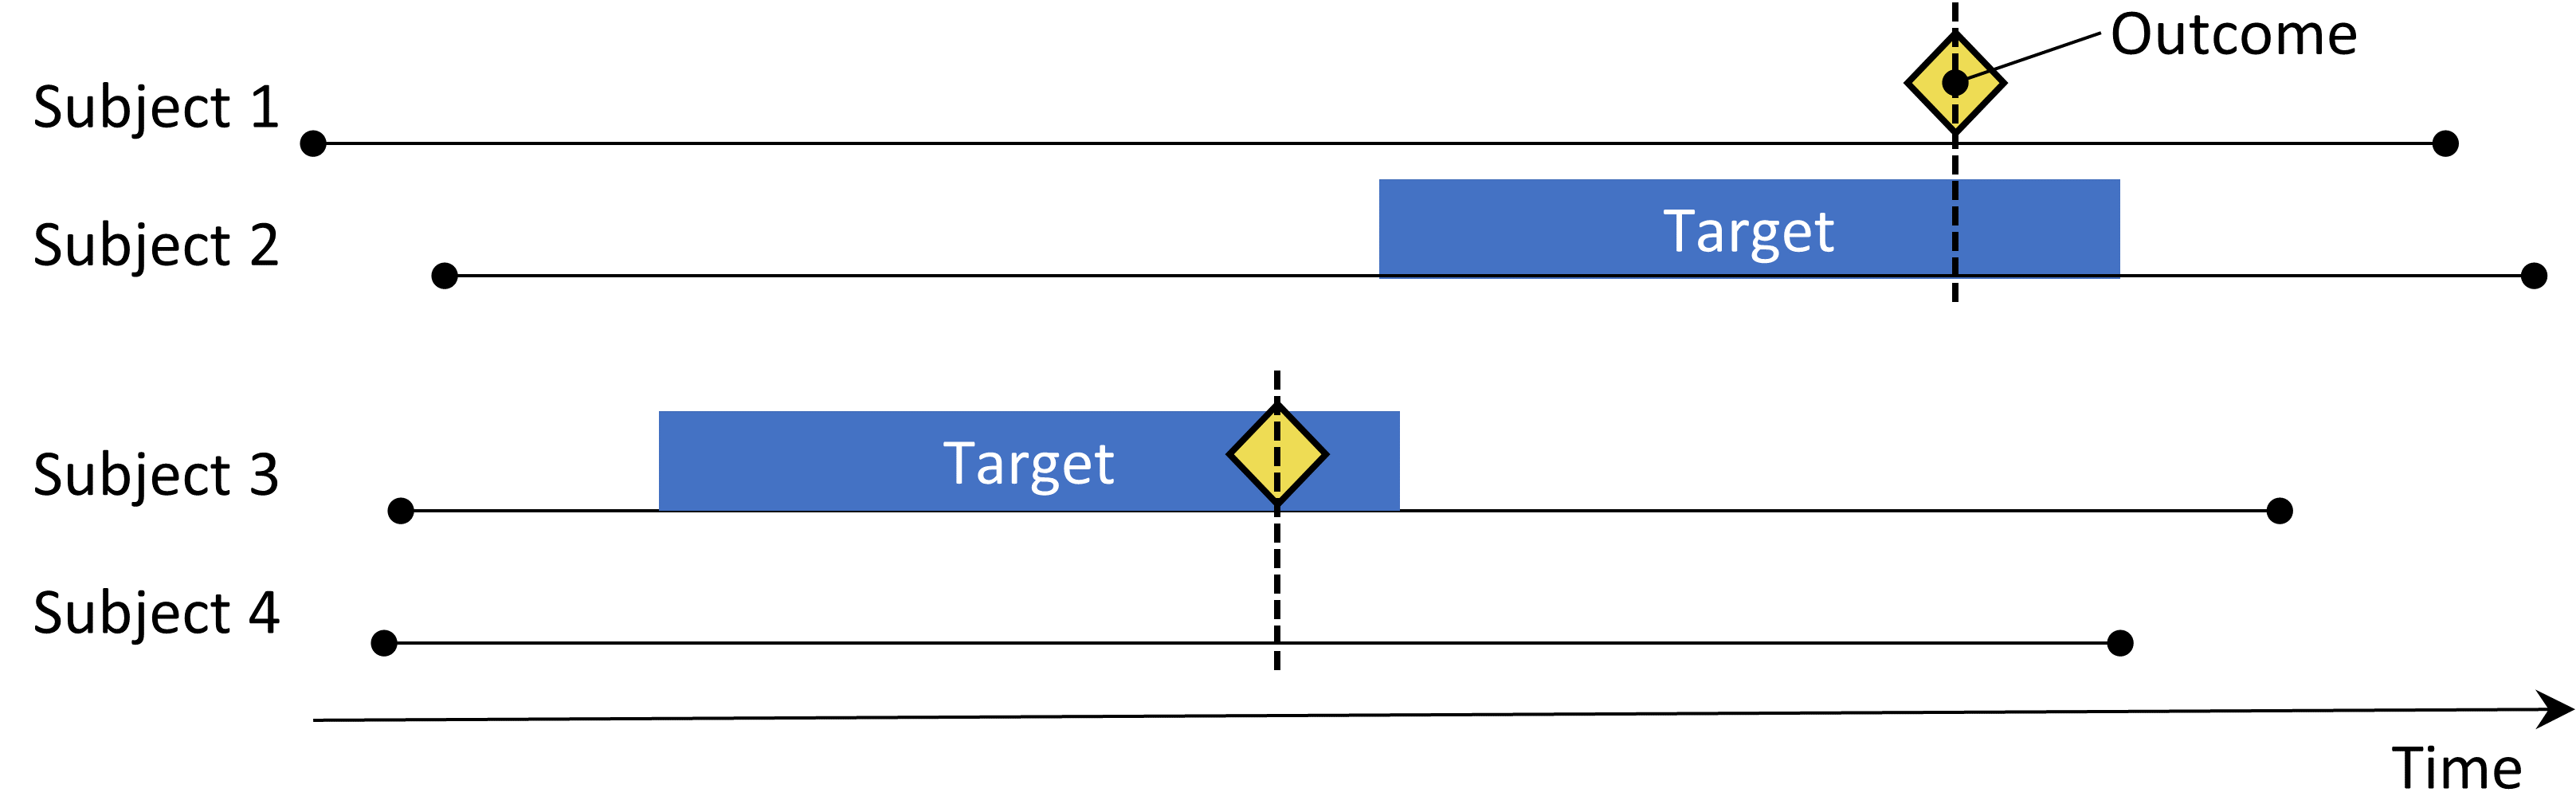
\includegraphics[width=0.9\linewidth]{images/PopulationLevelEstimation/caseControl} 

}

\caption{The case-control design. Subjects with the outcome (‘cases’) are compared to subjects without the outcome (‘controls’) in terms of their exposure status. Often, cases and controls are matched on various characteristics such as age and sex.}\label{fig:caseControl}
\end{figure}

Case-control studies \citep{vandenbroucke_2012} consider the question
``are persons with a specific disease outcome exposed more frequently to
a specific agent than those without the disease?'' Thus, the central
idea is to compare ``cases'', i.e., subjects that experience the outcome
of interest with ``controls'', i.e., subjects that did not experience
the outcome of interest. The choices in Table \ref{tab:ccChoices} define
a case-control question.

\begin{longtable}[]{@{}ll@{}}
\caption{\label{tab:ccChoices} Main design choices in a case-control
design.}\tabularnewline
\toprule
\begin{minipage}[b]{0.23\columnwidth}\raggedright\strut
Choice\strut
\end{minipage} & \begin{minipage}[b]{0.71\columnwidth}\raggedright\strut
Description\strut
\end{minipage}\tabularnewline
\midrule
\endfirsthead
\toprule
\begin{minipage}[b]{0.23\columnwidth}\raggedright\strut
Choice\strut
\end{minipage} & \begin{minipage}[b]{0.71\columnwidth}\raggedright\strut
Description\strut
\end{minipage}\tabularnewline
\midrule
\endhead
\begin{minipage}[t]{0.23\columnwidth}\raggedright\strut
Outcome cohort\strut
\end{minipage} & \begin{minipage}[t]{0.71\columnwidth}\raggedright\strut
A cohort representing the cases (the outcome of interest)\strut
\end{minipage}\tabularnewline
\begin{minipage}[t]{0.23\columnwidth}\raggedright\strut
Control cohort\strut
\end{minipage} & \begin{minipage}[t]{0.71\columnwidth}\raggedright\strut
A cohort representing the controls. Typically the control cohort is
automatically derived from the outcome cohort using some selection
logic\strut
\end{minipage}\tabularnewline
\begin{minipage}[t]{0.23\columnwidth}\raggedright\strut
Target cohort\strut
\end{minipage} & \begin{minipage}[t]{0.71\columnwidth}\raggedright\strut
A cohort representing the treatment\strut
\end{minipage}\tabularnewline
\begin{minipage}[t]{0.23\columnwidth}\raggedright\strut
{[}Nesting cohort{]}\strut
\end{minipage} & \begin{minipage}[t]{0.71\columnwidth}\raggedright\strut
Optionally, a cohort defining the subpopulation from which cases and
controls are drawn\strut
\end{minipage}\tabularnewline
\begin{minipage}[t]{0.23\columnwidth}\raggedright\strut
Time-at-risk\strut
\end{minipage} & \begin{minipage}[t]{0.71\columnwidth}\raggedright\strut
At what time (often relative to the index date) do we consider exposure
status?\strut
\end{minipage}\tabularnewline
\bottomrule
\end{longtable}

Often, one selects controls to match cases based on characteristics such
as age and sex to make them more comparable. Another widespread practice
is to nest the analysis within a specific subgroup of people, for
example people that have all been diagnosed with one of the indications
of the exposure of interest.

\section{The case-crossover design}\label{the-case-crossover-design}

\begin{figure}

{\centering 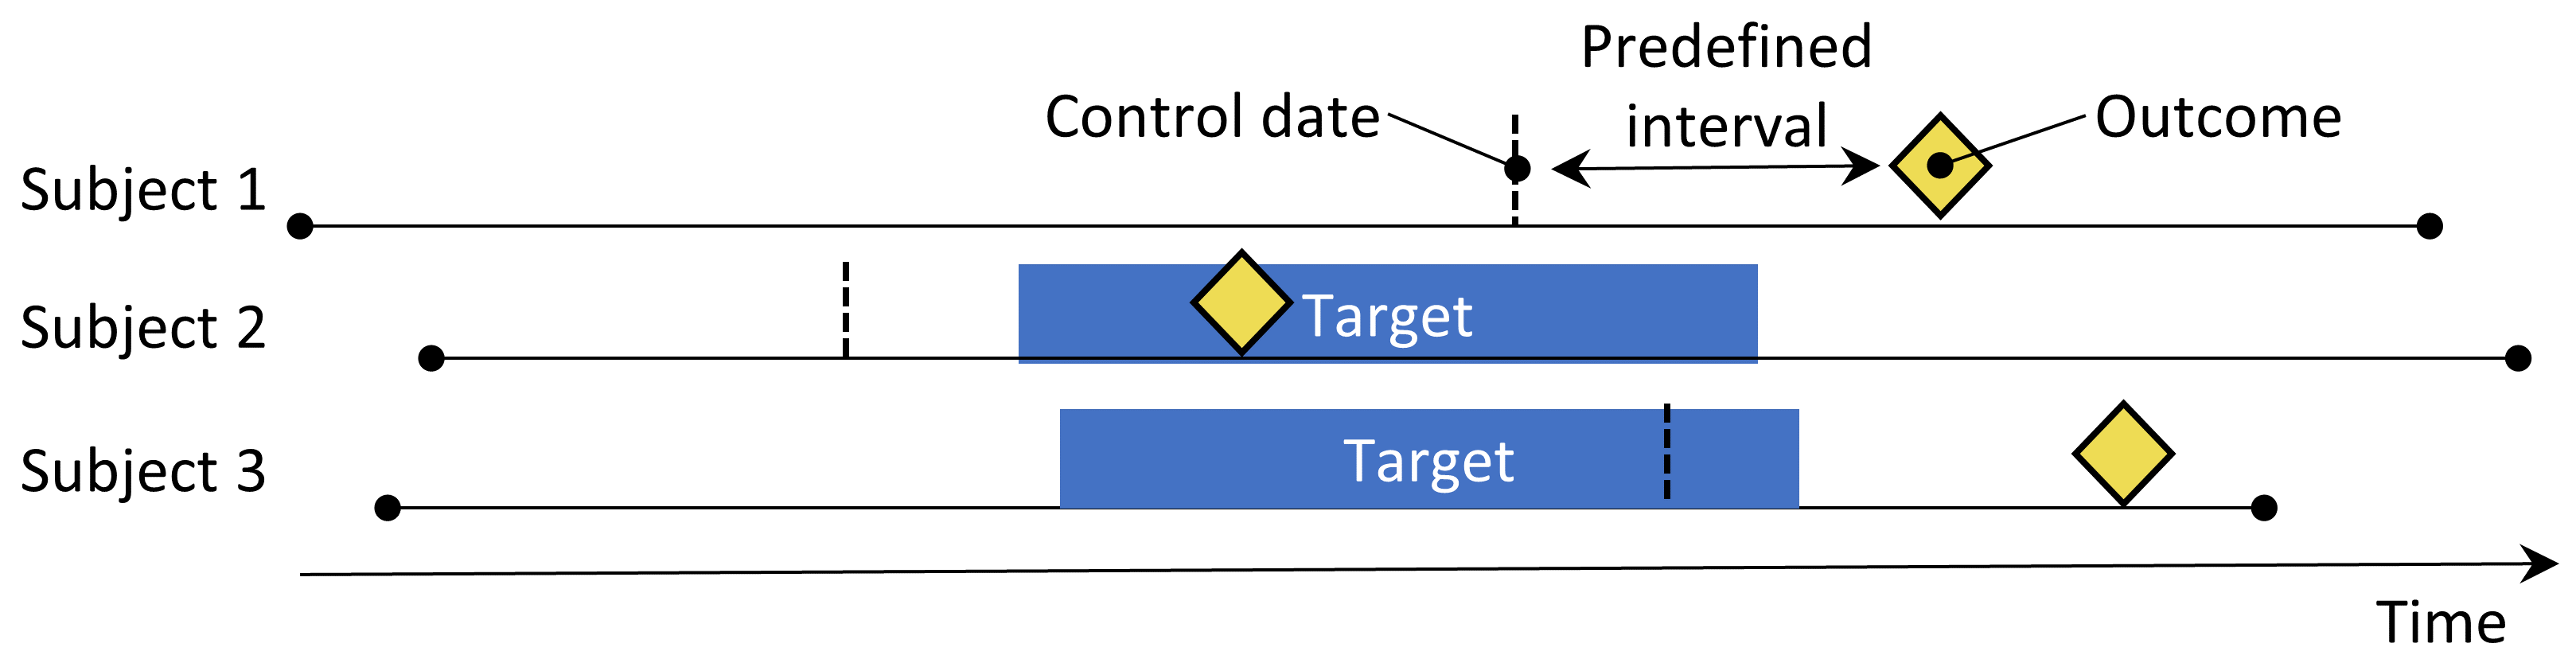
\includegraphics[width=0.9\linewidth]{images/PopulationLevelEstimation/caseCrossover} 

}

\caption{The case-crossover design. The time around the outcome is compared to a control date set at a predefined interval prior to the outcome date.}\label{fig:caseCrossover}
\end{figure}

The case-crossover \citep{maclure_1991} design evaluates whether the
rate of exposure is different at the time of the outcome than at some
predefined number of days prior to the outcome. It is trying to
determine whether there is something special about the day the outcome
occurred. Table \ref{tab:ccrChoices} shows the choices that define a
case-crossover question:

\begin{longtable}[]{@{}ll@{}}
\caption{\label{tab:ccrChoices} Main design choices in a case-crossover
design.}\tabularnewline
\toprule
\begin{minipage}[b]{0.23\columnwidth}\raggedright\strut
Choice\strut
\end{minipage} & \begin{minipage}[b]{0.71\columnwidth}\raggedright\strut
Description\strut
\end{minipage}\tabularnewline
\midrule
\endfirsthead
\toprule
\begin{minipage}[b]{0.23\columnwidth}\raggedright\strut
Choice\strut
\end{minipage} & \begin{minipage}[b]{0.71\columnwidth}\raggedright\strut
Description\strut
\end{minipage}\tabularnewline
\midrule
\endhead
\begin{minipage}[t]{0.23\columnwidth}\raggedright\strut
Outcome cohort\strut
\end{minipage} & \begin{minipage}[t]{0.71\columnwidth}\raggedright\strut
A cohort representing the cases (the outcome of interest)\strut
\end{minipage}\tabularnewline
\begin{minipage}[t]{0.23\columnwidth}\raggedright\strut
Target cohort\strut
\end{minipage} & \begin{minipage}[t]{0.71\columnwidth}\raggedright\strut
A cohort representing the treatment\strut
\end{minipage}\tabularnewline
\begin{minipage}[t]{0.23\columnwidth}\raggedright\strut
Time-at-risk\strut
\end{minipage} & \begin{minipage}[t]{0.71\columnwidth}\raggedright\strut
At what time (often relative to the index date) do we consider exposure
status?\strut
\end{minipage}\tabularnewline
\begin{minipage}[t]{0.23\columnwidth}\raggedright\strut
Control time\strut
\end{minipage} & \begin{minipage}[t]{0.71\columnwidth}\raggedright\strut
The time period used as the control time\strut
\end{minipage}\tabularnewline
\bottomrule
\end{longtable}

Since cases serve as their own control, it is a self-controlled design,
and should therefore be robust to confounding due to between-person
differences. One concern is that, because the outcome date is always
later than the control date, the method will be positively biased if the
overall frequency of exposure increases over time (or negatively biased
if there is a decrease). To address this, the case-time-control design
\citep{suissa_1995} was developed, which adds controls, matched for
example on age and sex, to the case-crossover design to adjust for
exposure trends.

\section{The self-controlled case series
design}\label{the-self-controlled-case-series-design}

\begin{figure}

{\centering 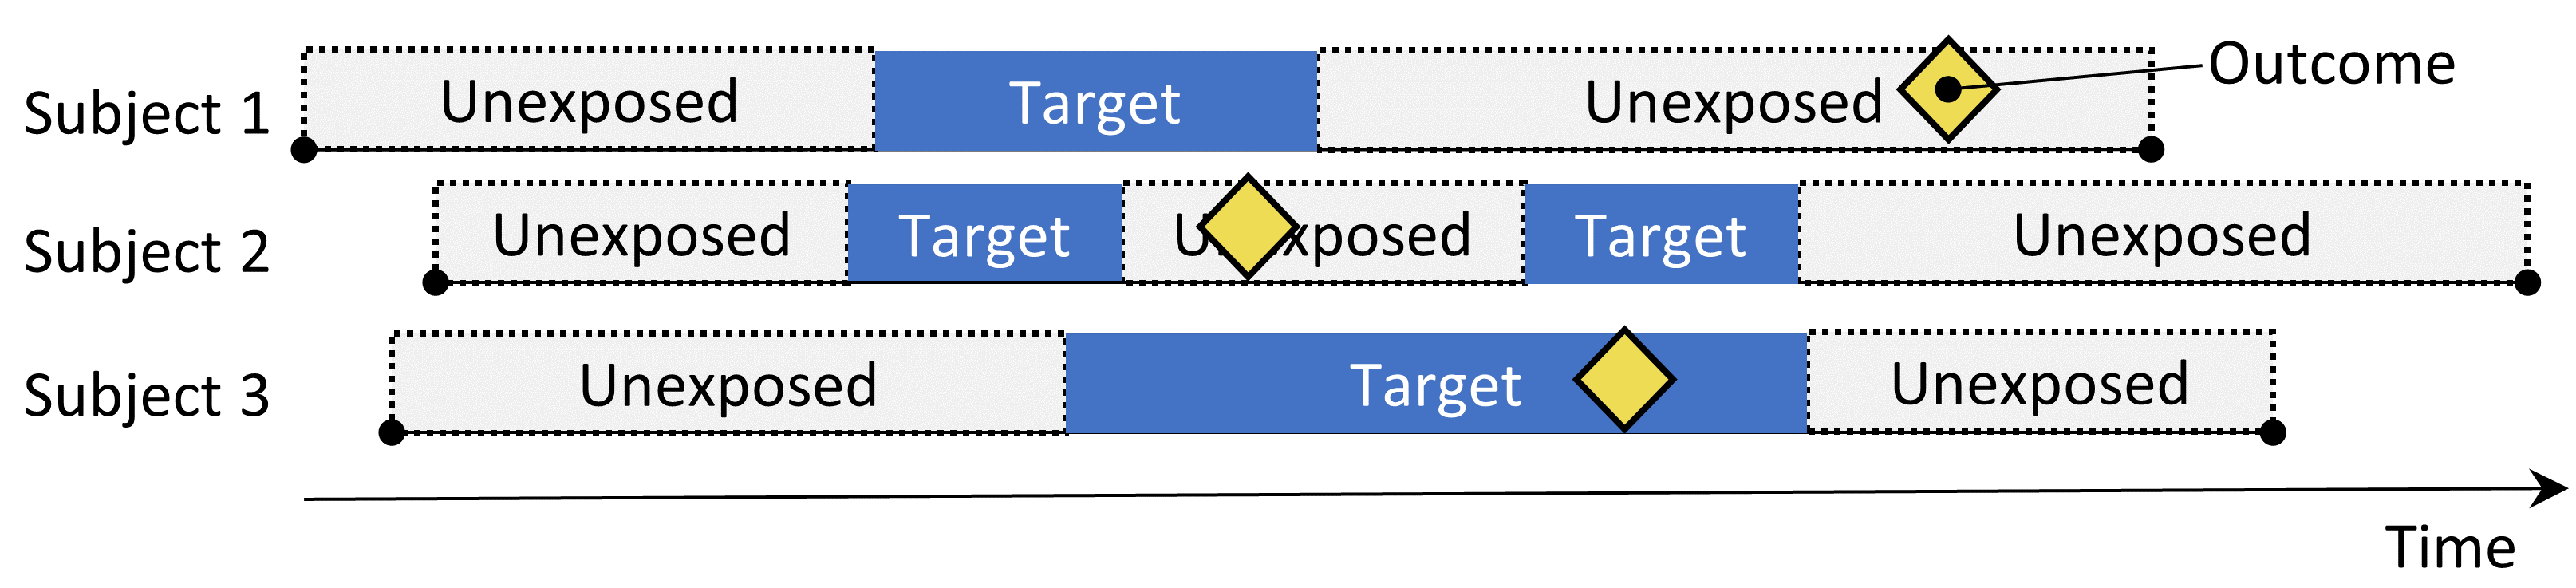
\includegraphics[width=0.9\linewidth]{images/PopulationLevelEstimation/selfControlledCaseSeries} 

}

\caption{The Self-Controlled Case Series design. The rate of outcomes during exposure is compared to the rate of outcomes when not exposed.}\label{fig:selfControlledCaseSeries}
\end{figure}

The Self-Controlled Case Series (SCCS) design
\citep{farrington_1995, whitaker_2006} compares the rate of outcomes
during exposure to the rate of outcomes during all unexposed time, both
before, between, and after exposures. It is a Poisson regression that is
conditioned on the person. Thus, it seeks to answer the question:
``Given that a patient has the outcome, is the outcome more likely
during exposed time compared to non-exposed time?''. The choices in
Table \ref{tab:sccsChoices} define an SCCS question.

\begin{longtable}[]{@{}ll@{}}
\caption{\label{tab:sccsChoices} Main design choices in a self-controlled
case series design.}\tabularnewline
\toprule
\begin{minipage}[b]{0.23\columnwidth}\raggedright\strut
Choice\strut
\end{minipage} & \begin{minipage}[b]{0.71\columnwidth}\raggedright\strut
Description\strut
\end{minipage}\tabularnewline
\midrule
\endfirsthead
\toprule
\begin{minipage}[b]{0.23\columnwidth}\raggedright\strut
Choice\strut
\end{minipage} & \begin{minipage}[b]{0.71\columnwidth}\raggedright\strut
Description\strut
\end{minipage}\tabularnewline
\midrule
\endhead
\begin{minipage}[t]{0.23\columnwidth}\raggedright\strut
Target cohort\strut
\end{minipage} & \begin{minipage}[t]{0.71\columnwidth}\raggedright\strut
A cohort representing the treatment\strut
\end{minipage}\tabularnewline
\begin{minipage}[t]{0.23\columnwidth}\raggedright\strut
Outcome cohort\strut
\end{minipage} & \begin{minipage}[t]{0.71\columnwidth}\raggedright\strut
A cohort representing the outcome of interest\strut
\end{minipage}\tabularnewline
\begin{minipage}[t]{0.23\columnwidth}\raggedright\strut
Time-at-risk\strut
\end{minipage} & \begin{minipage}[t]{0.71\columnwidth}\raggedright\strut
At what time (often relative to the target cohort start and end dates)
do we consider the risk of the outcome?\strut
\end{minipage}\tabularnewline
\begin{minipage}[t]{0.23\columnwidth}\raggedright\strut
Model\strut
\end{minipage} & \begin{minipage}[t]{0.71\columnwidth}\raggedright\strut
The model to estimate the effect, including any adjustments for
time-varying confounders\strut
\end{minipage}\tabularnewline
\bottomrule
\end{longtable}

Like other self-controlled designs, the SCCS is robust to confounding
due to between-person differences, but vulnerable to confounding due to
time-varying effects. Several adjustments are possible to attempt to
account for these, for example by including age and season. A special
variant of the SCCS includes not just the exposure of interest, but all
other exposures to drugs recorded in the database, \citep{simpson_2013}
potentially adding thousands of additional variables to the model.
L1-regularization using cross-validation to select the regularization
hyperparameter is applied to the coefficients of all exposures except
the exposure of interest.

One important assumption underlying the SCCS is that the observation
period end is independent of the date of the outcome. Because for some
outcomes, especially ones that can be fatal such as stroke, this
assumption can be violated. An extension to the SCCS has been developed
that corrects for any such dependency. \citep{farrington_2011}

\section{Designing a hypertension
study}\label{designing-a-hypertension-study}

\subsection{Problem definition}\label{problem-definition-1}

ACE inhibitors (ACEi) are widely used in patients with hypertension or
ischemic heart disease, especially those with other comorbidities such
as congestive heart failure, diabetes mellitus, or chronic kidney
disease. \citep{zaman_2002} Angioedema, a serious and sometimes
life-threatening adverse event that usually manifests as swelling of the
lips, tongue, mouth, larynx, pharynx, or periorbital region, has been
linked to the use of these medications. \citep{sabroe_1997} However,
limited information is available about the absolute and relative risks
for angioedema associated with the use of these medications. Existing
evidence is primarily based on investigations of specific cohorts (e.g.,
predominantly male veterans or Medicaid beneficiaries), whose findings
may not be generalizable to other populations, or based on
investigations with few events, which provide unstable risk estimates
\citep{powers_2012}. Several observational studies compare ACEi to
beta-blockers for the risk of angioedema, \citep{magid_2010, toh_2012}
but beta-blockers are no longer recommend as first-line treatment of
hypertension. \citep{whelton_2018} A viable alternative treatment could
be thiazides or thiazide-like diuretics (THZ), which could be just as
effective in managing hypertension and its associated risks such as
acute myocardial infarction (AMI), but without increasing the risk of
angioedema.

The following will demonstrate how to apply our population-level
estimation framework to observational healthcare data to address the
following comparative estimation questions:

\begin{quote}
What is the risk of angioedema in new users of ACE inhibitors compared
to new users of thiazide and thiazide-like diuretics?
\end{quote}

\begin{quote}
What is the risk of acute myocaridal infarction in new users of ACE
inhibitors compared to new users of thiazide and thiazide-like
diuretics?
\end{quote}

Since these are comparative effect estimation questions we will apply
the cohort method as described in Section \ref{CohortMethod}.

\subsection{Target and comparator}\label{target-and-comparator}

We consider patients new-users if their first observed treatment for
hypertension was monotherapy with any active ingredient in either the
ACEi or THZ class. We define mono therapy as not starting on any other
anti-hypertensive drug in the seven days following treatment initiation.
We require patients to have at least one year of prior continuous
observation in the database before first exposure and a recorded
hypertension diagnosis at or in the year preceding treatment initiation.

\subsection{Outcome}\label{outcome-1}

We define angioedema as any occurrence of an angioedema condition
concept during an inpatient or emergency room (ER) visit, and require
there to be no angioedema diagnosis recorded in the seven days prior. We
define AMI as any occurrence of an AMI condition concept during an
inpatient or ER visit, and require there to be no AMI diagnosis record
in the 180 days prior.

\subsection{Time-at-risk}\label{time-at-risk-1}

We define time-at-risk to start on the day after treatment initiation,
and stop when exposure stops, allowing for a 30-day gap between
subsequent drug exposures.

\subsection{Model}\label{model}

We fit a PS model using the default set of covariates, including
demographics, conditions, drugs, procedures, measurements, observations,
and several co-morbidity scores. We exclude ACEi and THZ from the
covariates. We perform variable-ratio matching and condition the Cox
regression on the matched sets.

\subsection{Study summary}\label{study-summary}

\begin{longtable}[]{@{}ll@{}}
\caption{\label{tab:aceChoices} Main design choices four our comparative
cohort study.}\tabularnewline
\toprule
\begin{minipage}[b]{0.23\columnwidth}\raggedright\strut
Choice\strut
\end{minipage} & \begin{minipage}[b]{0.71\columnwidth}\raggedright\strut
Value\strut
\end{minipage}\tabularnewline
\midrule
\endfirsthead
\toprule
\begin{minipage}[b]{0.23\columnwidth}\raggedright\strut
Choice\strut
\end{minipage} & \begin{minipage}[b]{0.71\columnwidth}\raggedright\strut
Value\strut
\end{minipage}\tabularnewline
\midrule
\endhead
\begin{minipage}[t]{0.23\columnwidth}\raggedright\strut
Target cohort\strut
\end{minipage} & \begin{minipage}[t]{0.71\columnwidth}\raggedright\strut
New users of ACE inhibitors as first-line monotherapy for
hypertension.\strut
\end{minipage}\tabularnewline
\begin{minipage}[t]{0.23\columnwidth}\raggedright\strut
Comparator cohort\strut
\end{minipage} & \begin{minipage}[t]{0.71\columnwidth}\raggedright\strut
New users of thiazides or thiazide-like diuretics as first-line
monotherapy for hypertension.\strut
\end{minipage}\tabularnewline
\begin{minipage}[t]{0.23\columnwidth}\raggedright\strut
Outcome cohort\strut
\end{minipage} & \begin{minipage}[t]{0.71\columnwidth}\raggedright\strut
Angioedema or acute myocardial infarction.\strut
\end{minipage}\tabularnewline
\begin{minipage}[t]{0.23\columnwidth}\raggedright\strut
Time-at-risk\strut
\end{minipage} & \begin{minipage}[t]{0.71\columnwidth}\raggedright\strut
Starting the day after treatment initiation, stopping when exposure
stops.\strut
\end{minipage}\tabularnewline
\begin{minipage}[t]{0.23\columnwidth}\raggedright\strut
Model\strut
\end{minipage} & \begin{minipage}[t]{0.71\columnwidth}\raggedright\strut
Cox proportional hazards model using variable-ratio matching.\strut
\end{minipage}\tabularnewline
\bottomrule
\end{longtable}

\subsection{Control questions}\label{control-questions}

To evaluate whether our study design produces estimates in line with the
truth, we additionally include a set of control questions where the true
effect size is known. Control questions can be divided in negative
controls, having a hazard ratio of 1, and positive controls, having a
known hazard ratio greater than 1. For several reasons we use real
negative controls, and synthesize positive controls based on these
negative controls. How to define and use control questions is discussed
in detail in Chapter \ref{MethodValidity}.

\section{Implementing the study using
ATLAS}\label{implementing-the-study-using-atlas}

Here we demonstrate how this study can be implemented using the
Estimation function in ATLAS. Click on
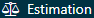
\includegraphics{images/PopulationLevelEstimation/estimation.png} in the
left bar of ATLAS, and create a new estimation study. Make sure to give
the study an easy-to-recognize name. The study design can be saved at
any time by clicking the

\includegraphics{images/PopulationLevelEstimation/save.png} button.

In the Estimation design function, there are three sections:
Comparisons, Analysis Settings, and Evaluation Settings. We can specify
multiple comparisons and multiple analysis settings, and ATLAS will
execute all combinations of these as separate analyses. Here we discuss
each section:

\subsection{Comparative cohort settings}\label{ComparisonSettings}

A study can have one or more comparisons. Click on ``Add Comparison'',
which will open a new dialog. Click on

\includegraphics{images/PopulationLevelEstimation/open.png} to the
select the target and comparator cohorts. By clicking on ``Add Outcome''
we can add our two outcome cohorts. We assume the cohorts have already
been created in ATLAS as described in Chapter \ref{Cohorts}. The
Appendix provides the full definitions of the target (Appendix
\ref{AceInhibitorsMono}) , comparator (Appendix \ref{ThiazidesMono}),
and outcome (Appendix \ref{Angioedema} and Appendix \ref{Ami}) cohorts.
When done, the dialog should look like Figure \ref{fig:comparisons}.

\begin{figure}

{\centering 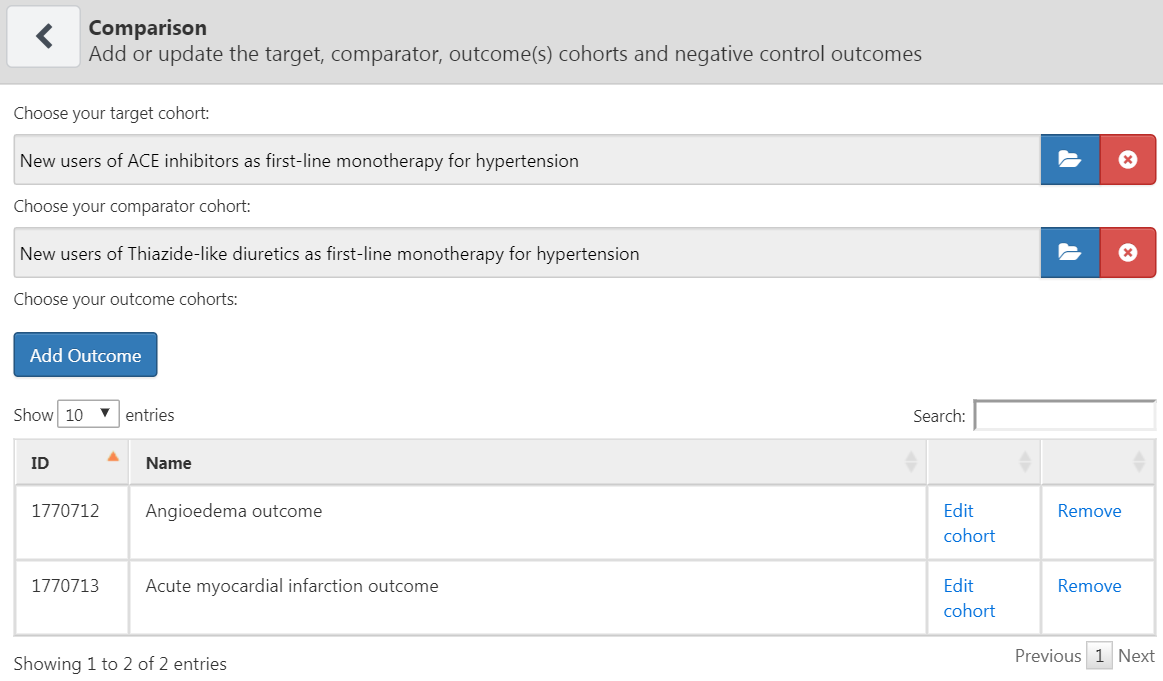
\includegraphics[width=1\linewidth]{images/PopulationLevelEstimation/comparisons} 

}

\caption{The comparison dialog}\label{fig:comparisons}
\end{figure}

Note that we can select multiple outcomes for a target-comparator pair.
Each outcome will be treated independently, and will result in a
separate analysis.

\textbf{Negative control outcomes}

Negative controls outcomes are outcomes that are not believed to be
caused by either the target or the comparator, and where therefore the
true hazard ratio equals 1. Ideally, we would have proper cohort
definitions for each outcome cohort. However, typically, we only have a
concept set, with one concept per negative control outcome, and some
standard logic to turn these into outcome cohorts. Here we assume the
concept set has already been created as described in Chapter
\ref{MethodValidity} and can simply be selected. The negative control
concept set should contain a concept per negative control, and not
include descendants. Figure \ref{fig:ncConceptSet} shows the negative
control concept set used for this study.

\begin{figure}

{\centering 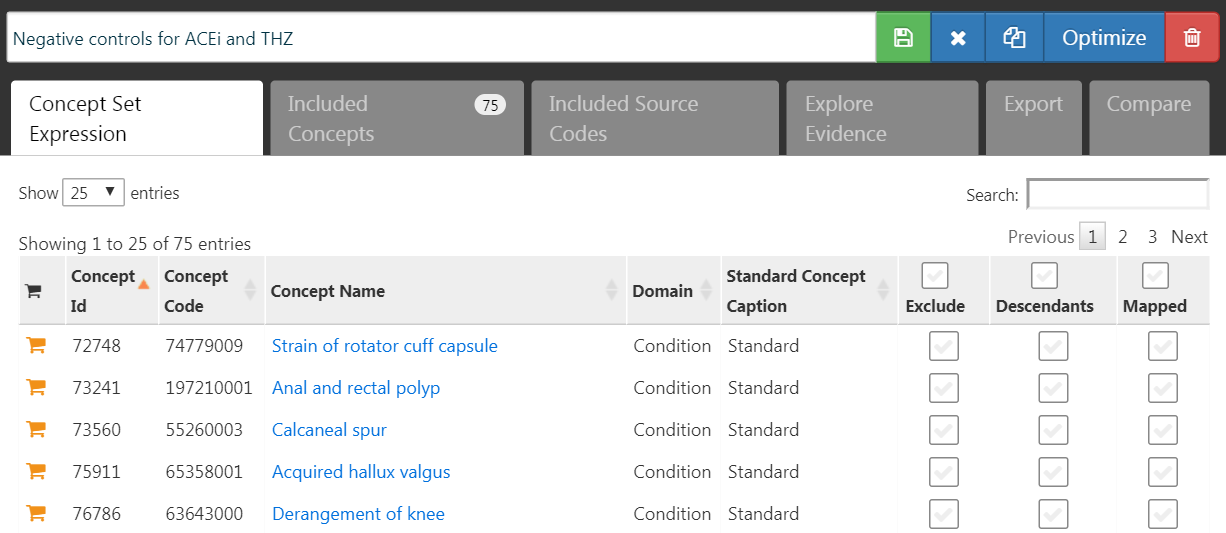
\includegraphics[width=1\linewidth]{images/PopulationLevelEstimation/ncConceptSet} 

}

\caption{Negative Control concept set.}\label{fig:ncConceptSet}
\end{figure}

\textbf{Concepts to include}

TODO: Update these sections when ATLAS interface has been updated.

When selecting concept to include, we can specify which covariates we
would like to generate, for example to use in a propensity model. When
specifying covariates here, all other covariates (aside from those you
specified) are left out. We usually want to include all baseline
covariates, letting the regularized regression build a model that
balances all covariates. The only reason we might want to specify
particular covariates is to replicate an existing study that manually
picked covariates. These inclusions can be specified in this comparison
section or in the analysis section, because sometimes they pertain to a
specific comparison (e.g.~know confounders in a comparison), or
sometimes they pertain to an analysis (e.g.~when evaluating a particular
covariate selection strategy).

\textbf{Concepts to exclude}

Rather than specifying which concepts to include, we can instead specify
concepts to \emph{exclude}. When we submit a concept set in this field,
we use every covariate except for those that we submitted. When using
the default set of covariates, which includes all drugs and procedures
occurring on the day of treatment initiation, we must exclude the target
and comparator treatment, and any concepts that are directly related to
these. For example, if the target exposure is an injectable, we should
not only exclude the drug, but also the injection procedure from the
propensity model. In this example, the covariates we want to exclude are
ACEi and THZ. Figure \ref{fig:covsToExclude} shows we select a concept
set that includes all these concepts.

\begin{figure}

{\centering 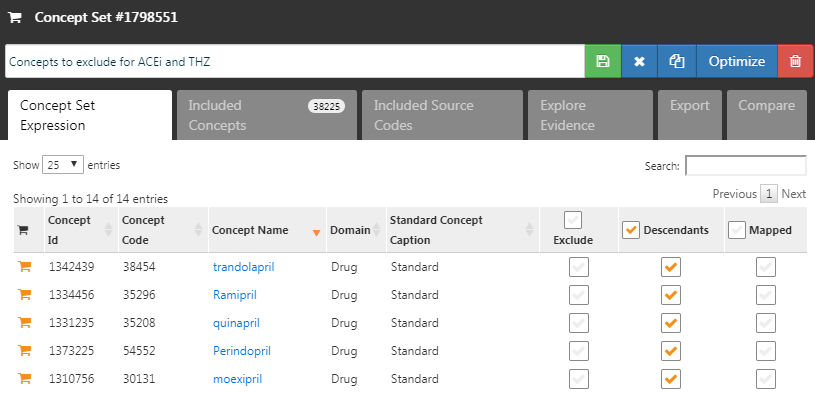
\includegraphics[width=1\linewidth]{images/PopulationLevelEstimation/covsToExclude} 

}

\caption{The concept set defining the concepts to exclude.}\label{fig:covsToExclude}
\end{figure}

After selecting the negative controls and covariates to exclude, the
lower half of the comparisons dialog should look like Figure
\ref{fig:comparisons2}.

\begin{figure}

{\centering 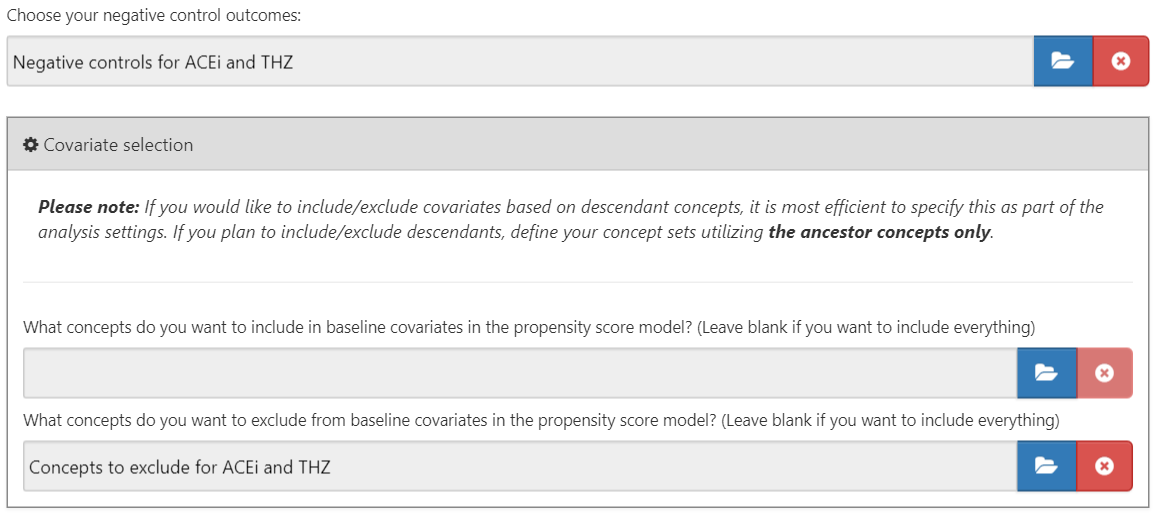
\includegraphics[width=1\linewidth]{images/PopulationLevelEstimation/comparisons2} 

}

\caption{The comparison window showing concept sets for negative controls and concepts to exclude.}\label{fig:comparisons2}
\end{figure}

\subsection{Effect estimation analysis
settings}\label{effect-estimation-analysis-settings}

After closing the comparisons dialog we can click on ``Add Analysis
Settings''. In the box labeled ``Analysis Name'', we can give the
analysis a unique name that is easy to remember and locate in the
future. For example, we could set the name to ``Propensity score
matching''.

\textbf{Study population}

There are a wide range of options to specify the study population; the
set of subjects that will enter the analysis. Many of these overlap with
options available when designing the target and comparator cohorts in
the cohort definition tool. One reason for using the options in
Estimation instead of in the cohort definition is re-usability: We can
define the target, comparator, and outcome cohorts completely
independently, and add dependencies between these at a later point in
time. For example, if we wish to remove people who had the outcome
before treatment initiation, we could do so in the definitions of the
target and comparator cohort, but then we would need to create separate
cohorts for every outcome! Instead, we can choose to have people with
prior outcomes be removed in the analysis settings, and now we can reuse
our target and comparator cohorts for our two outcomes of interest (as
well as our negative control outcomes).

The \textbf{study start and end dates} can be used to limit the analyses
to a specific period. The study end date also truncates risk windows,
meaning no outcomes beyond the study end date will be considered. One
reason for selecting a study start date might be that one of the drugs
being studied is new and did not exist in an earlier time. Automatically
adjusting for this can be done by answering ``yes'' to the question
``\textbf{Restrict the analysis to the period when both exposures are
observed?}''. Another reason to adjust study start and end dates might
be that medical practice changed over time (e.g., due to a drug warning)
and we are only interested in the time where medicine was practiced a
specific way.

The option ``\textbf{Should only the first exposure per subject be
included?}'' can be used to restrict to the first exposure per patient.
Often this is already done in the cohort definition, as is the case in
this example. Similarly, the option ``\textbf{The minimum required
continuous observation time prior to index date for a person to be
included in the cohort}'' is often already set in the cohort definition,
and can therefore be left at 0 here. Having observed time (as defined in
the OBSERVATION\_PERIOD table) before the index date ensures that there
is sufficient information about the patient to calculate a propensity
score, and is also often used to ensure the patient is truly a new user,
and therefore was not exposed before.

``\textbf{Remove subjects that are in both the target and comparator
cohort?}'' defines, together with the option ``\textbf{If a subject is
in multiple cohorts, should time-at-risk be censored when the new
time-at-risk starts to prevent overlap?}'' what happens when a subject
is in both target and comparator cohort. The first setting has three
choices:

\begin{itemize}
\tightlist
\item
  ``\textbf{Keep All}'' indicating to keep the subjects in both cohorts.
  With this option it might be possible to double-count subjects and
  outcomes.
\item
  ``\textbf{Keep First}'' indicating to keep the subject in the first
  cohort that occurred.
\item
  ``\textbf{Remove All}'' indicating to remove the subject from both
  cohorts.
\end{itemize}

If the options ``keep all'' or ``keep first'' are selected, we may wish
to censor the time when a person is in both cohorts. This is illustrated
in Figure \ref{fig:tar}. By default, the time-at-risk is defined
relative to the cohort start and end date. In this example, the
time-at-risk starts one day after cohort entry, and stops at cohort end.
Without censoring the time-at-risk for the two cohorts might overlap.
This is especially problematic if we choose to keep all, because any
outcome that occurs during this overlap (as shown) will be counted
twice. If we choose to censor, the first cohort's time-at-risk ends when
the second cohort's time-at-risk starts.

\begin{figure}

{\centering 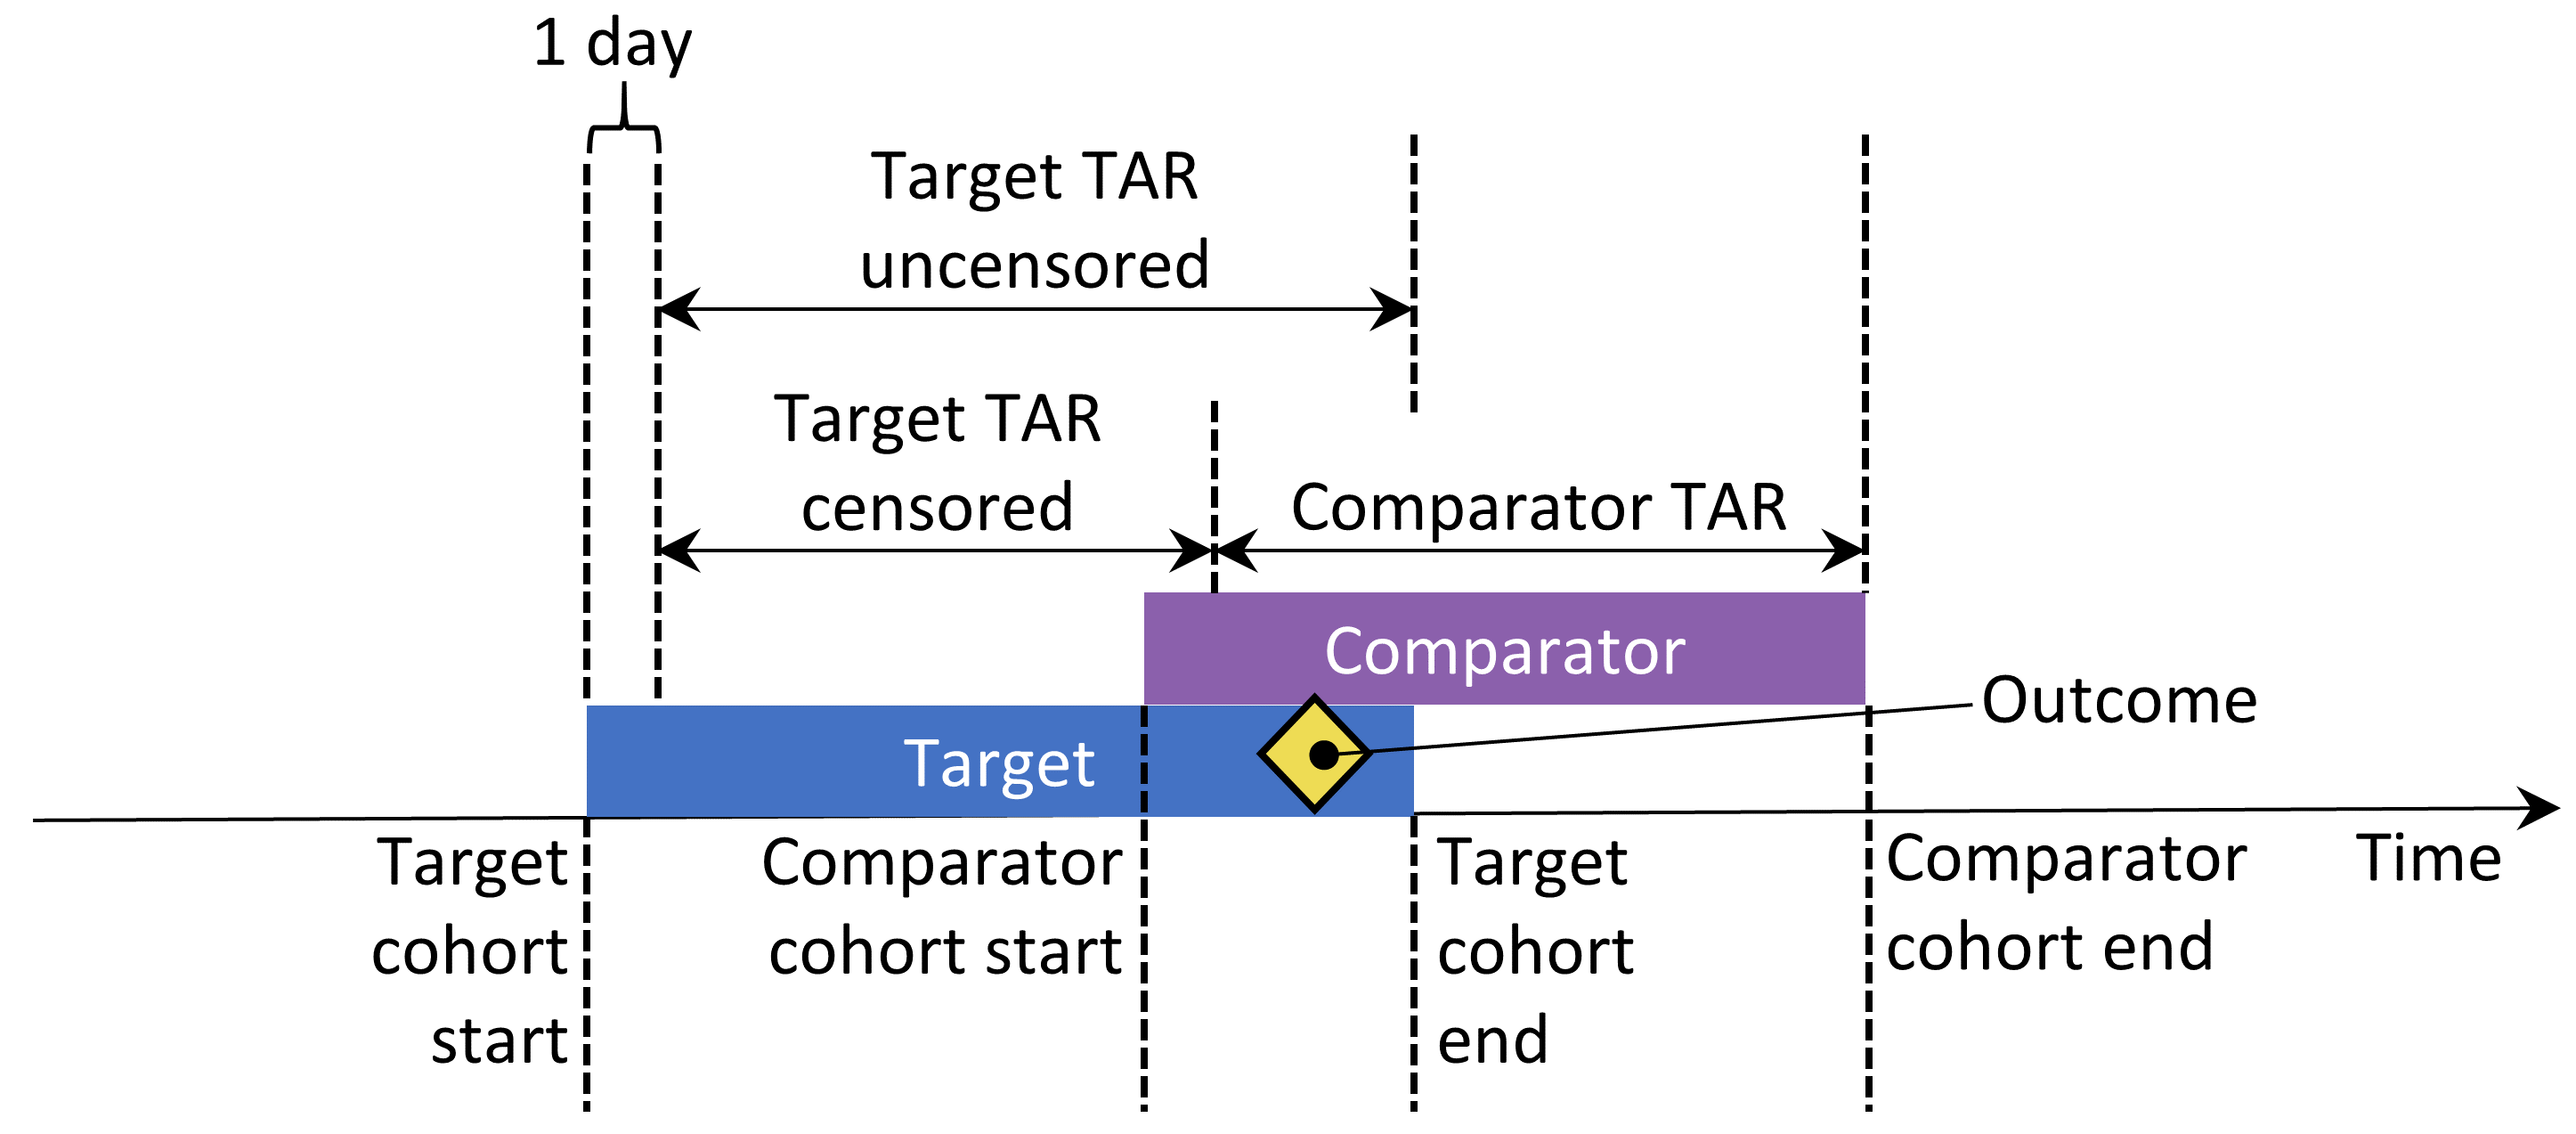
\includegraphics[width=0.8\linewidth]{images/PopulationLevelEstimation/tar} 

}

\caption{Time-at-risk (TAR) for subjects who are in both cohorts, assuming time-at-risk starts the day after treatment initiation, and stops at exposure end.}\label{fig:tar}
\end{figure}

We can choose to \textbf{remove subjects that have the outcome prior to
the risk window start}, because often a second outcome occurrence is the
continuation of the first one. For instance, when someone develops heart
failure, a second occurrence is likely, which means the heart failure
probably never fully resolved in between. On the other hand, some
outcomes are episodic, and it would be expected for patients to have
more than one independent occurrence, like an upper respiratory
infection. If we choose to remove people that had the outcome before, we
can select \textbf{how many days we should look back when identifying
prior outcomes}.

Our choices for our example study are shown in Figure
\ref{fig:studyPopulation}. Because our target and comparator cohort
definitions already restrict to the first exposure and require
observation time prior to treatment initiation, we do not apply these
criteria here.

\begin{figure}

{\centering 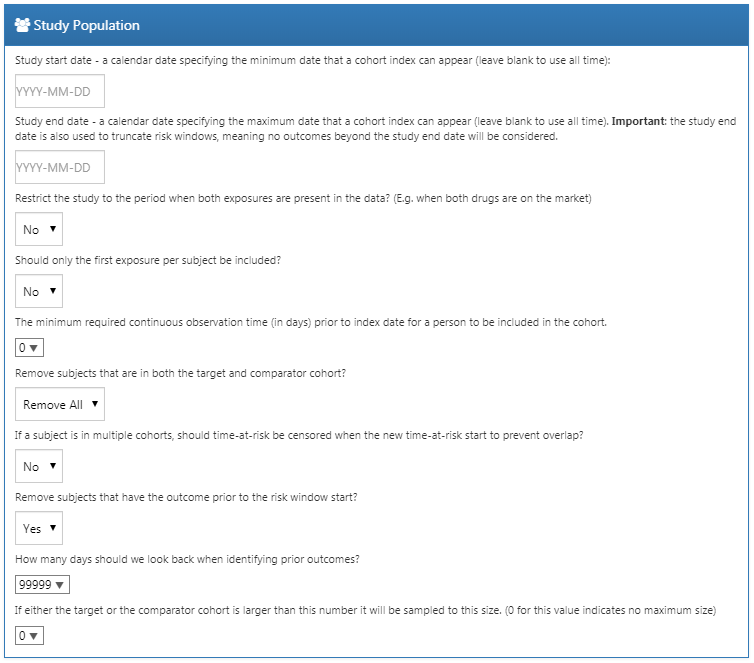
\includegraphics[width=1\linewidth]{images/PopulationLevelEstimation/studyPopulation} 

}

\caption{Study population settings..}\label{fig:studyPopulation}
\end{figure}

\textbf{Covariate settings}

Here we specify the covariates to construct. These covariates are
typically used in the propensity model, but can also be included in the
outcome model (the Cox proporitional hazards model in this case). If we
\textbf{click to view details} of our covariate settings, we can select
which sets of covariates to construct. However, the recommendation is to
use the default set, which constructs covariates for demographics, all
conditions, drugs, procedures, measurements, etc.

We can modify the set of covariates by specifying concepts to
\textbf{include} and/or \textbf{exclude}. These settings are the same as
the ones found in Section \ref{ComparisonSettings} on comparison
settings. The reason why they can be found in two places is because
sometimes these settings are related to a specific comparison, as is the
case here because we wish to exclude the drugs we are comparing, and
sometimes the settings are related to a specific analysis. When
executing an analysis for a specific comparison using specific analysis
settings, the OHDSI tools will take the union of these sets.

The choice to \textbf{add descendants to include or exclude} affects
this union of the two settings. So in this example we specified only the
ingredients to exclude when defining the comparisons. Here we set
``Should descendant concepts be added to the list of excluded
concepts?'' to ``Yes'' to also add all descendants.

Figure \ref{fig:covariateSettings} shows our choices for this study.
Note that we have selected to add descendants to the concept to exclude,
which we defined in the comparison settings in Figure
\ref{fig:comparisons2}.

\begin{figure}

{\centering 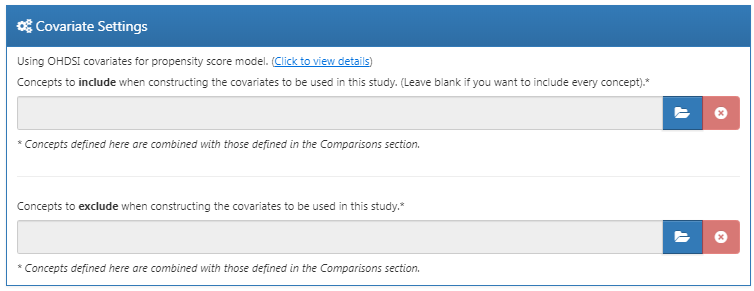
\includegraphics[width=1\linewidth]{images/PopulationLevelEstimation/covariateSettings} 

}

\caption{Covariate settings.}\label{fig:covariateSettings}
\end{figure}

\textbf{Time at risk}

Time-at-risk is defined relative to the start and end dates of our
target and comparator cohorts. In our example, we had set the cohort
start date to start on treatment initiation, and cohort end date when
exposure stops (for at least 30 days). We set the start of time-at-risk
to one day after cohort start, so one day after treatment initiation. A
reason to set the time-at-risk start to be later than the cohort start
is because we may want to exclude outcome events that occur on the day
of treatment initiation if we do not believe it biologically plausible
they can be caused by the drug.

We set the end of the time-at-risk to the cohort end, so when exposure
stops. We could choose to set the end date later if for example we
believe events closely following treatment end may still be attributable
to the exposure. In the extreme we could set the time-at-risk end to a
large number of days (e.g.~99999) after the cohort end date, meaning we
will effectively follow up subjects until observation end. Such a design
is sometimes referred to as an \emph{intent-to-treat} design.

A patient with zero days at risk adds no information, so the
\textbf{minimum days at risk} is normally set at one day. If there is a
known latency for the side effect, then this may be increased to get a
more informative proportion. It can also be used to create a cohort more
similar to that of a randomized trial it is being compared to (e.g., all
the patients in the randomized trial were observed for at least N days).

\BeginKnitrBlock{rmdimportant}
A golden rule in designing a cohort study is to never use information
that falls after the cohort start date to define the study population,
as this may introduce bias. For example, if we require everyone to have
at least a year of time-at-risk, we will likely have limited our
analyses to those who tolerate the treatment well. This setting should
therefore be used with extreme care.
\EndKnitrBlock{rmdimportant}

\begin{figure}

{\centering 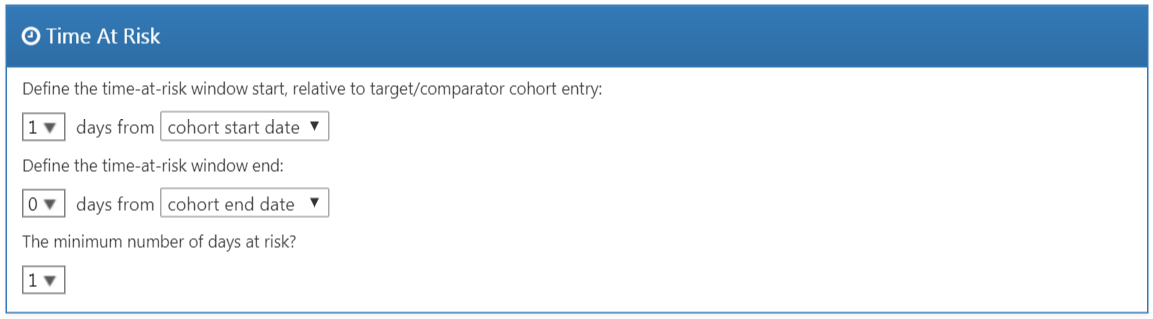
\includegraphics[width=1\linewidth]{images/PopulationLevelEstimation/timeAtRisk} 

}

\caption{Time-at-risk settings.}\label{fig:timeAtRisk}
\end{figure}

\textbf{Propensity score adjustment}

We can opt to \textbf{trim} the study population, removing people with
extreme PS values. We can choose to remove the top and bottom
percentage, or we can remove subjects whose preference score falls
outside the range we specify. Trimming the cohorts is generally not
recommended because it requires discarding observations, which reduces
statistical power. It may be desirable to trim in some cases, for
example when using IPTW.

In addition to, or instead of trimming, we can choose to
\textbf{stratify} or \textbf{match} on the propensity score. When
stratifying we need to specify the \textbf{number of strata} and whether
to select the strata based on the target, comparator, or entire study
population. When matching we need to specify the \textbf{maximum number
of people from the comparator group to match to each person in the
target group}. Typical values are 1 for one-on-one matching, or a large
number (e.g.~100) for variable-ratio matching. We also need to specify
the \textbf{caliper}: the maximum allowed difference between propensity
scores to allow a match. The caliper can be defined on difference
\textbf{caliper scales}:

\begin{itemize}
\tightlist
\item
  \textbf{The propensity score scale}: the PS itself
\item
  \textbf{The standardized scale}: in standard deviations of the PS
  distributions
\item
  \textbf{The standardized logit scale}: in standard deviations of the
  PS distributions after the logit transformation to make the PS more
  normally distributed.
\end{itemize}

In case of doubt, we suggest using the default values, or consult the
work on this topic by \citet{austin_2011}.

Fitting large-scale propensity models can be computationally expensive,
so we may want to restrict the data used to fit the model to just a
sample of the data. By default the maximum size of the target and
comparator cohort is set to 250,000. In most studies this limit will not
be reached. It is also unlikely that more data will lead to a better
model. Note that although a sample of the data may be used to fit the
model, the model will be used to compute PS for the entire population.

\textbf{Test each covariate for correlation with the target assignment?}
If any covariate has an unusually high correlation (either positive or
negative), this will throw an error. This avoids lengthy calculation of
a propensity model only to discover complete separation. Finding very
high univariate correlation allows you to review the covariate to
determine why it has high correlation and whether it should be dropped.

Figure \ref{fig:psSettings} shows our choices for this study. Note that
we select variable-ratio matching by setting the maximum number of
people to match to 100.

\begin{figure}

{\centering 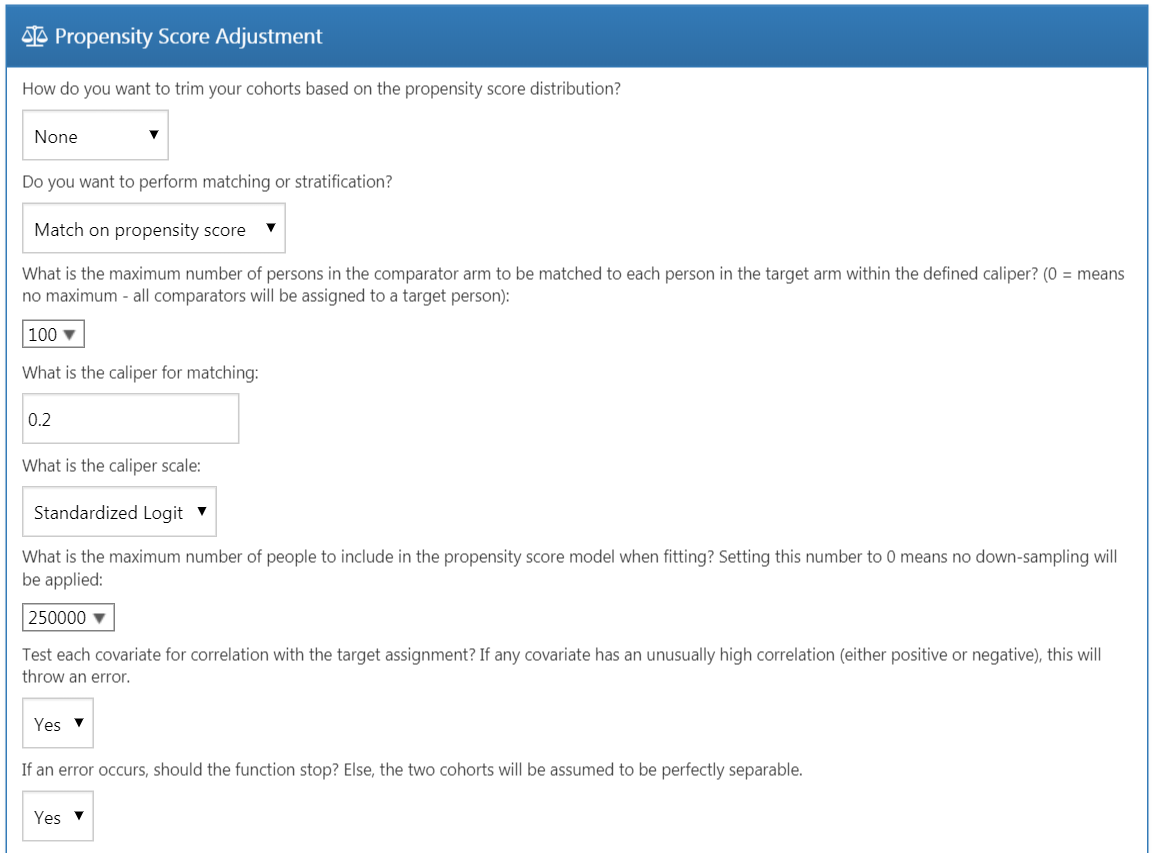
\includegraphics[width=1\linewidth]{images/PopulationLevelEstimation/psSettings} 

}

\caption{Propenstity score adjustment settings.}\label{fig:psSettings}
\end{figure}

\textbf{Outcome model settings}

First, we need to \textbf{specify the statistical model we will use to
estimate the relative risk of the outcome between target and comparator
cohorts}. We can choose between Cox, Poisson, and logistic regression,
as discussed briefly in Section \ref{CohortMethod}. For our example we
choose a Cox proportional hazards model, which considers time to first
event with possible censoring. Next, we need to specify \textbf{whether
the regression should be conditioned on the strata}. One way to
understand conditioning is to imagine a separate estimate is produced in
each stratum, and then combined across strata. For one-to-one matching
this is likely unnecessary and would just lose power. For stratification
or variable-ratio matching it is required.

We can also choose to \textbf{add all covariates to the outcome model}
to adjust the analysis. This can be done in addition or instead of using
a propensity model. However, whereas there usually is ample data to fit
a propensity model, with many people in both treatment groups, there is
typically very little data to fit the outcome model, with only few
people having the outcome. We therefore recommend keeping the outcome
model as simple as possible and not include additional covariates.

Instead of stratifying or matching on the propensity score we can also
choose to \textbf{use inverse probability of treatment weighting}
(IPTW). If weighting is used it is often recommended to use some form of
trimming to avoid extreme weights and therefore unstable estimates.

Figure \ref{fig:psSettings} shows our choices for this study. Because we
use variable-ratio matching, we must condition the regression on the
strata (i.e.~the matched sets).

\begin{figure}

{\centering 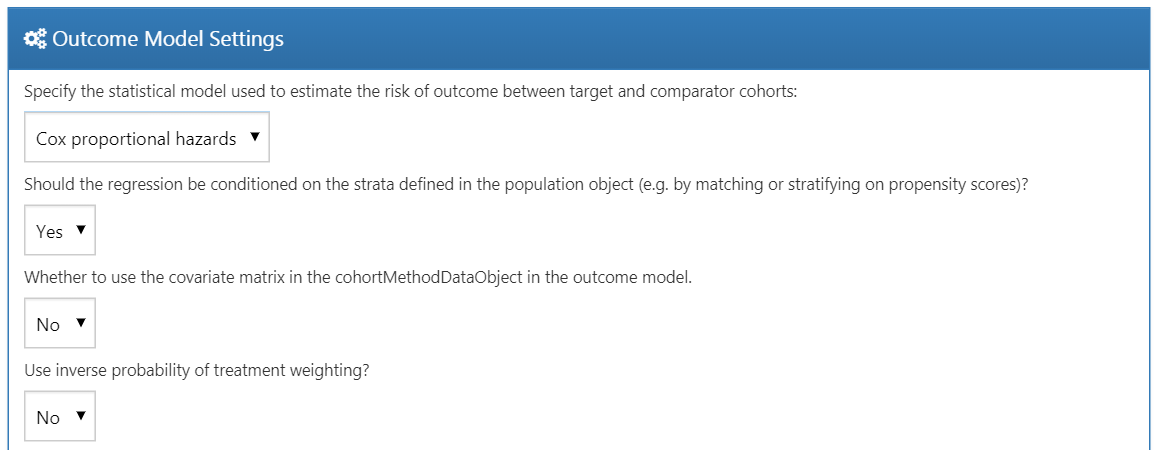
\includegraphics[width=1\linewidth]{images/PopulationLevelEstimation/outcomeModelSettings} 

}

\caption{Outcome model settings.}\label{fig:outcomeModelSettings}
\end{figure}

\subsection{Evaluation settings}\label{evaluationSettings}

As described in Chapter \ref{MethodValidity}, negative and positive
controls should be included in our study to evaluate the operating
characteristics, and perform empirical calibration.

\textbf{Negative control outcome cohort definition}

In Section \ref{ComparisonSettings} we selected a concept set
representing the negative control outcomes. However, we need logic to
convert concepts to cohorts to be used as outcomes in our analysis.
ATLAS provides standard logic with three choices The first choice is
whether to \textbf{use all occurrences} or just the \textbf{first
occurrence} of the concept. The second choice determines \textbf{whether
occurrences of descendant concepts should be considered}. For example,
occurrences of the descendant ``ingrown nail of foot'' can also be
counted as an occurrence of the ancestor ``ingrown nail''. The third
choice specifies which domains should be considered when looking for the
concepts.

\begin{figure}

{\centering 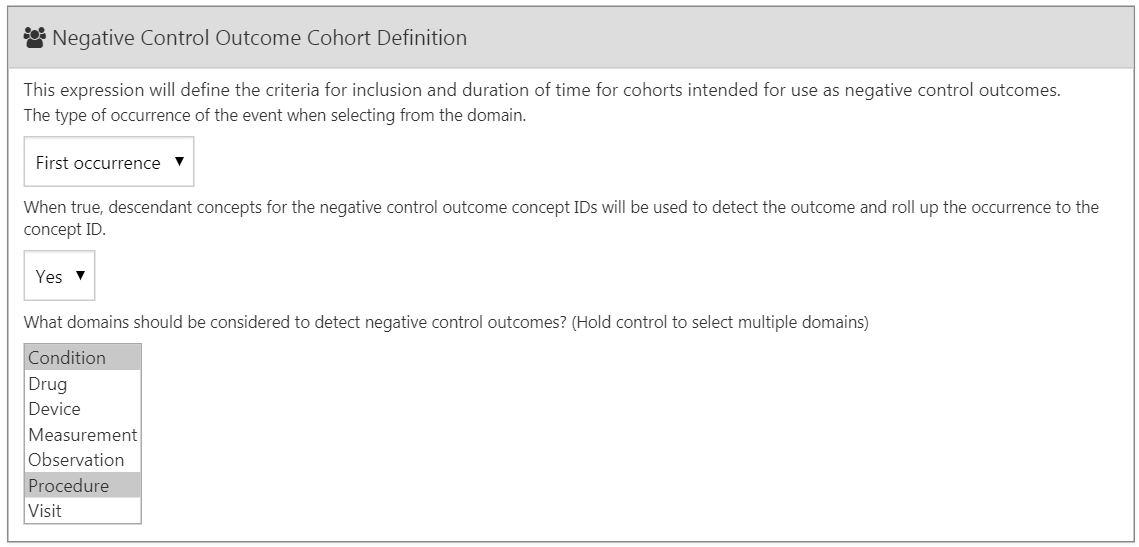
\includegraphics[width=1\linewidth]{images/PopulationLevelEstimation/ncSettings} 

}

\caption{Negative control outcome cohort definition settings.}\label{fig:ncSettings}
\end{figure}

\textbf{Positive control synthesis}

In addition to negative controls we can also include positive controls,
which are exposure-outcome pairs where a causal effect is believed to
exist with known effect size. For various reasons real positive controls
are problematic, so instead we rely on synthetic positive controls,
derived from negative controls as described in Chapter
\ref{MethodValidity}. Positive control synthesis is an advanced topic
that we will skip for now.

TODO: Add positive control synthesis settings when ATLAS interface is
updated.

\subsection{Running the study package}\label{running-the-study-package}

Now that we have fully defined our study, we can export it as an
executable R package. This package contains everything that is needed to
execute the study at a site that has data in CDM. This includes the
cohort definitions that can be used to instantiate the target,
comparator and outcome cohorts, the negative control concept set and
logic to create the negative control outcome cohorts, as well as the R
code to execute the analysis. Before generating the package make sure to
save your study, then click on the \textbf{Utilities} tab. Here we can
review the set of analyses that will be performed. As mentioned before,
every combination of a comparison and an analysis setting will results
in a separate analysis. In our example we have specified two analyses:
ACEi versus THZ for AMI, and ACEi versus THZ for angioedema, both using
propensity score matching.

We must provide a name for our package, after which we can click on
``Download'' to download the zip file. The zip file contains an R
package, with the usual required folder structure for R packages.
\citep{Wickham_2015} To use this package we recommend using R Studio. If
you are running R Studio locally, unzip the file, and double click the
.Rproj file to open it in R Studio. If you are running R Studio on an R
studio server, click

\includegraphics{images/PopulationLevelEstimation/upload.png} to upload
and unzip the file, then click on the .Rproj file to open the project.

Once you have opened the project in R Studio, you can open the README
file, and follow the instructions. Make sure to change all file paths to
existing paths on your system.

A common error message that may appear when running the study is ``High
correlation between covariate(s) and treatment detected''. This
indicates that when fitting the propensity model, some covariates were
observed to be highly correlated with the exposure. Please review the
covariates mentioned in the error message, and exclude them from the set
of covariates if appropriate (see Section \ref{VariableSelection}).

\section{Implementing the study using
R}\label{implementing-the-study-using-r}

Instead of using ATLAS to write the R code that executes the study, we
can also write the R code ourselves. One reason we might want to do this
is because R offers far greater flexibility than is exposed in ATLAS. If
we for example wish to use custom covariates, or a linear outcome model,
we will need to write some custom R code, and combine it with the
functionality provided by the OHDSI R packages.

For our example study we will rely on the
\href{https://ohdsi.github.io/CohortMethod/}{CohortMethod} package to
execute our study. CohortMethod extracts the necessary data from a
database in the CDM and can use a large set of covariates for the
propensity model. In the following example we first only consider
angioedema as outcome. In Section \ref{MultipleAnalyses} we then
describe how this can be extended to include AMI and the negative
control outcomes.

\subsection{Cohort instantiation}\label{cohort-instantiation}

We first need to instantiate the target and outcome cohorts.
Instantiating cohorts is described in Chapter \ref{Cohorts}. The
Appendix provides the full definitions of the target (Appendix
\ref{AceInhibitorsMono}), comparator (Appendix \ref{ThiazidesMono}), and
outcome (Appendix \ref{Angioedema} ) cohorts. We will assume the ACEi,
THZ, and angioedema cohorts have been instantiated in a table called
\texttt{scratch.my\_cohorts} with cohort definition IDs 1,2, and 3
respectively.

\subsection{Data extraction}\label{data-extraction}

We first need to tell R how to connect to the server.
\href{https://ohdsi.github.io/CohortMethod/}{CohortMethod} uses the
\href{https://ohdsi.github.io/DatabaseConnector/}{DatabaseConnector}
package, which provides a function called
\texttt{createConnectionDetails}. Type \texttt{?createConnectionDetails}
for the specific settings required for the various database management
systems (DBMS). For example, one might connect to a PostgreSQL database
using this code:

\begin{Shaded}
\begin{Highlighting}[]
\KeywordTok{library}\NormalTok{(CohortMethod)}
\NormalTok{connDetails <-}\StringTok{ }\KeywordTok{createConnectionDetails}\NormalTok{(}\DataTypeTok{dbms =} \StringTok{"postgresql"}\NormalTok{,}
                                       \DataTypeTok{server =} \StringTok{"localhost/ohdsi"}\NormalTok{,}
                                       \DataTypeTok{user =} \StringTok{"joe"}\NormalTok{,}
                                       \DataTypeTok{password =} \StringTok{"supersecret"}\NormalTok{)}

\NormalTok{cdmDbSchema <-}\StringTok{ "my_cdm_data"}
\NormalTok{cohortsDbSchema <-}\StringTok{ "scratch"}
\NormalTok{cohortsDbTable <-}\StringTok{ "my_cohorts"}
\NormalTok{cdmVersion <-}\StringTok{ "5"}
\end{Highlighting}
\end{Shaded}

The last four lines define the \texttt{cdmDbSchema},
\texttt{cohortsDbSchema}, and \texttt{cohortsDbTable} variables, as well
as the CDM version. We will use these later to tell R where the data in
CDM format live, where the cohorts of interest have been created, and
what version CDM is used. Note that for Microsoft SQL Server, database
schemas need to specify both the database and the schema, so for example
\texttt{cdmDbSchema\ \textless{}-\ "my\_cdm\_data.dbo"}.

Now we can tell CohortMethod to extract the cohorts, construct
covariates, and extract all necessary data for our analysis:

\begin{Shaded}
\begin{Highlighting}[]
\CommentTok{# target and comparator ingredient concepts:}
\NormalTok{aceI <-}\StringTok{ }\KeywordTok{c}\NormalTok{(}\DecValTok{1335471}\NormalTok{,}\DecValTok{1340128}\NormalTok{,}\DecValTok{1341927}\NormalTok{,}\DecValTok{1363749}\NormalTok{,}\DecValTok{1308216}\NormalTok{,}\DecValTok{1310756}\NormalTok{,}\DecValTok{1373225}\NormalTok{,}
          \DecValTok{1331235}\NormalTok{,}\DecValTok{1334456}\NormalTok{,}\DecValTok{1342439}\NormalTok{)}
\NormalTok{thz <-}\StringTok{ }\KeywordTok{c}\NormalTok{(}\DecValTok{1395058}\NormalTok{,}\DecValTok{974166}\NormalTok{,}\DecValTok{978555}\NormalTok{,}\DecValTok{907013}\NormalTok{)}

\CommentTok{# Define which types of covariates must be constructed:}
\NormalTok{cs <-}\StringTok{ }\KeywordTok{createDefaultCovariateSettings}\NormalTok{(}\DataTypeTok{excludedCovariateConceptIds =} \KeywordTok{c}\NormalTok{(aceI, }
\NormalTok{                                                                     thz),}
                                     \DataTypeTok{addDescendantsToExclude =} \OtherTok{TRUE}\NormalTok{)}

\CommentTok{#Load data:}
\NormalTok{cmData <-}\StringTok{ }\KeywordTok{getDbCohortMethodData}\NormalTok{(}\DataTypeTok{connectionDetails =}\NormalTok{ connectionDetails,}
                                \DataTypeTok{cdmDatabaseSchema =}\NormalTok{ cdmDatabaseSchema,}
                                \DataTypeTok{oracleTempSchema =} \OtherTok{NULL}\NormalTok{,}
                                \DataTypeTok{targetId =} \DecValTok{1}\NormalTok{,}
                                \DataTypeTok{comparatorId =} \DecValTok{2}\NormalTok{,}
                                \DataTypeTok{outcomeIds =} \DecValTok{3}\NormalTok{,}
                                \DataTypeTok{studyStartDate =} \StringTok{""}\NormalTok{,}
                                \DataTypeTok{studyEndDate =} \StringTok{""}\NormalTok{,}
                                \DataTypeTok{exposureDatabaseSchema =}\NormalTok{ cohortsDbSchema,}
                                \DataTypeTok{exposureTable =}\NormalTok{ cohortsDbTable,}
                                \DataTypeTok{outcomeDatabaseSchema =}\NormalTok{ cohortsDbSchema,}
                                \DataTypeTok{outcomeTable =}\NormalTok{ cohortsDbTable,}
                                \DataTypeTok{cdmVersion =}\NormalTok{ cdmVersion,}
                                \DataTypeTok{firstExposureOnly =} \OtherTok{FALSE}\NormalTok{,}
                                \DataTypeTok{removeDuplicateSubjects =} \OtherTok{FALSE}\NormalTok{,}
                                \DataTypeTok{restrictToCommonPeriod =} \OtherTok{FALSE}\NormalTok{,}
                                \DataTypeTok{washoutPeriod =} \DecValTok{0}\NormalTok{,}
                                \DataTypeTok{covariateSettings =}\NormalTok{ cs)}
\NormalTok{cmData}
\end{Highlighting}
\end{Shaded}

\begin{verbatim}
## CohortMethodData object
## 
## Treatment concept ID: 1
## Comparator concept ID: 2
## Outcome concept ID(s): 3
\end{verbatim}

There are many parameters, but they are all documented in the
\href{https://ohdsi.github.io/CohortMethod/reference/}{CohortMethod
manual}. The \texttt{createDefaultCovariateSettings} function is
described in the
\href{https://ohdsi.github.io/FeatureExtraction/}{FeatureExtraction}
package. In short, we are pointing the function to the table containing
our cohorts and specify which cohort definition IDs in that table
identify the target, comparator and outcome. We instruct that the
default set of covariates should be constructed, including covariates
for all conditions, drug exposures, and procedures that were found on or
before the index date. As mentioned in Section \ref{CohortMethod} we
must exclude the target and comparator treatments from the set of
covariates, and here we achieve this by listing all ingredients in the
two classes, and tell FeatureExtraction to also exclude all descendants,
thus excluding all drugs that contain these ingredients.

All data about the cohorts, outcomes, and covariates are extracted from
the server and stored in the \texttt{cohortMethodData} object. This
object uses the package \texttt{ff} to store information in a way that
ensures R does not run out of memory, even when the data are large, as
mentioned in Section \ref{BigDataSupport}.

We can use the generic \texttt{summary()} function to view some more
information of the data we extracted:

\begin{Shaded}
\begin{Highlighting}[]
\KeywordTok{summary}\NormalTok{(cmData)}
\end{Highlighting}
\end{Shaded}

\begin{verbatim}
## CohortMethodData object summary
## 
## Treatment concept ID: 1
## Comparator concept ID: 2
## Outcome concept ID(s): 3
## 
## Treated persons: 67166
## Comparator persons: 35333
## 
## Outcome counts:
##          Event count Person count
## 3               980          891
## 
## Covariates:
## Number of covariates: 58349
## Number of non-zero covariate values: 24484665
\end{verbatim}

Creating the \texttt{cohortMethodData} file can take considerable
computing time, and it is probably a good idea to save it for future
sessions. Because \texttt{cohortMethodData} uses \texttt{ff}, we cannot
use R's regular save function. Instead, we'll have to use the
\texttt{saveCohortMethodData()} function:

\begin{Shaded}
\begin{Highlighting}[]
\KeywordTok{saveCohortMethodData}\NormalTok{(cmData, }\StringTok{"AceiVsThzForAngioedema"}\NormalTok{)}
\end{Highlighting}
\end{Shaded}

We can use the \texttt{loadCohortMethodData()} function to load the data
in a future session.

\textbf{Defining new users}

Typically, a new user is defined as first time use of a drug (either
target or comparator), and typically a washout period (a minimum number
of days prior first use) is used to increase the probability that it is
truly first use. When using the CohortMethod package, you can enforce
the necessary requirements for new use in three ways:

\begin{enumerate}
\def\labelenumi{\arabic{enumi}.}
\tightlist
\item
  When defining the cohorts.
\item
  When loading the cohorts using the \texttt{getDbCohortMethodData}
  function, you can use the \texttt{firstExposureOnly},
  \texttt{removeDuplicateSubjects}, \texttt{restrictToCommonPeriod}, and
  \texttt{washoutPeriod} arguments.
\item
  When defining the study population using the
  \texttt{createStudyPopulation} function (see below) using the
  \texttt{firstExposureOnly}, \texttt{removeDuplicateSubjects},
  \texttt{restrictToCommonPeriod}, and \texttt{washoutPeriod} arguments.
\end{enumerate}

The advantage of option 1 is that the input cohorts are already fully
defined outside of the CohortMethod package, and external cohort
characterization tools can be used on the same cohorts used in this
analysis. The advantage of options 2 and 3 is that they save you the
trouble of limiting to first use yourself, for example allowing you to
directly use the DRUG\_ERA table in the CDM. Option 2 is more efficient
than 3, since only data for first use will be fetched, while option 3 is
less efficient but allows you to compare the original cohorts to the
study population.

\subsection{Defining the study
population}\label{defining-the-study-population}

Typically, the exposure cohorts and outcome cohorts will be defined
independently of each other. When we want to produce an effect size
estimate, we need to further restrict these cohorts and put them
together, for example by removing exposed subjects that had the outcome
prior to exposure, and only keeping outcomes that fall within a defined
risk window. For this we can use the \texttt{createStudyPopulation}
function:

\begin{Shaded}
\begin{Highlighting}[]
\NormalTok{studyPop <-}\StringTok{ }\KeywordTok{createStudyPopulation}\NormalTok{(}\DataTypeTok{cohortMethodData =}\NormalTok{ cmData,}
                                  \DataTypeTok{outcomeId =} \DecValTok{3}\NormalTok{,}
                                  \DataTypeTok{firstExposureOnly =} \OtherTok{FALSE}\NormalTok{,}
                                  \DataTypeTok{restrictToCommonPeriod =} \OtherTok{FALSE}\NormalTok{,}
                                  \DataTypeTok{washoutPeriod =} \DecValTok{0}\NormalTok{,}
                                  \DataTypeTok{removeDuplicateSubjects =} \StringTok{"remove all"}\NormalTok{,}
                                  \DataTypeTok{removeSubjectsWithPriorOutcome =} \OtherTok{TRUE}\NormalTok{,}
                                  \DataTypeTok{minDaysAtRisk =} \DecValTok{1}\NormalTok{,}
                                  \DataTypeTok{riskWindowStart =} \DecValTok{1}\NormalTok{,}
                                  \DataTypeTok{addExposureDaysToStart =} \OtherTok{FALSE}\NormalTok{,}
                                  \DataTypeTok{riskWindowEnd =} \DecValTok{0}\NormalTok{,}
                                  \DataTypeTok{addExposureDaysToEnd =} \OtherTok{TRUE}\NormalTok{)}
\end{Highlighting}
\end{Shaded}

Note that we've set \texttt{firstExposureOnly} and
\texttt{removeDuplicateSubjects} to FALSE, and \texttt{washoutPeriod} to
0 because we already applied those criteria in the cohort definitions.
We specify the outcome ID we will use, and that people with outcomes
prior to the risk window start date will be removed. The risk window is
defined as starting on the day after the cohort start date
(\texttt{riskWindowStart\ =\ 1} and
\texttt{addExposureDaysToStart\ =\ FALSE}), and the risk windows ends
when the cohort exposure ends (\texttt{riskWindowEnd\ =\ 0} and
\texttt{addExposureDaysToEnd\ =\ TRUE}), which was defined as the end of
exposure in the cohort definition. Note that the risk windows are
automatically truncated at the end of observation or the study end date.
We also remove subjects who have no time at risk. To see how many people
are left in the study population we can always use the
\texttt{getAttritionTable} function:

\begin{Shaded}
\begin{Highlighting}[]
\KeywordTok{getAttritionTable}\NormalTok{(studyPop)}
\end{Highlighting}
\end{Shaded}

\begin{verbatim}
##                    description targetPersons comparatorPersons           ...
## 1             Original cohorts         67212             35379           ...
## 2 Removed subs in both cohorts         67166             35333           ...
## 3             No prior outcome         67061             35238           ...
## 4 Have at least 1 days at risk         66780             35086           ...
\end{verbatim}

\subsection{Propensity scores}\label{propensity-scores-1}

We can fit a propensity model using the covariates constructed by the
\texttt{getDbcohortMethodData()} function, and compute a PS for each
person:

\begin{Shaded}
\begin{Highlighting}[]
\NormalTok{ps <-}\StringTok{ }\KeywordTok{createPs}\NormalTok{(}\DataTypeTok{cohortMethodData =}\NormalTok{ cmData, }\DataTypeTok{population =}\NormalTok{ studyPop)}
\end{Highlighting}
\end{Shaded}

The \texttt{createPs} function uses the
\href{https://ohdsi.github.io/Cyclops/}{Cyclops} package to fit a
large-scale regularized logistic regression. To fit the propensity
model, Cyclops needs to know the hyperparameter value which specifies
the variance of the prior. By default Cyclops will use cross-validation
to estimate the optimal hyperparameter. However, be aware that this can
take a really long time. You can use the \texttt{prior} and
\texttt{control} parameters of the \texttt{createPs} function to specify
Cyclops' behavior, including using multiple CPUs to speed-up the
cross-validation.

Here we use the PS to perform variable-ratio matching:

\begin{Shaded}
\begin{Highlighting}[]
\NormalTok{matchedPop <-}\StringTok{ }\KeywordTok{matchOnPs}\NormalTok{(}\DataTypeTok{population =}\NormalTok{ ps, }\DataTypeTok{caliper =} \FloatTok{0.2}\NormalTok{, }
                        \DataTypeTok{caliperScale =} \StringTok{"standardized logit"}\NormalTok{, }\DataTypeTok{maxRatio =} \DecValTok{100}\NormalTok{)}
\end{Highlighting}
\end{Shaded}

Alternatively, we could have used the PS in the \texttt{trimByPs},
\texttt{trimByPsToEquipoise}, or \texttt{stratifyByPs} functions.

\subsection{Outcome models}\label{outcome-models}

The outcome model is a model describing which variables are associated
with the outcome. Under strict assumptions, the coefficient for the
treatment variable can be interpreted as the causal effect. In this case
we fit a Cox proportional hazards model, conditioned (stratified) on the
matched sets:

\begin{Shaded}
\begin{Highlighting}[]
\NormalTok{outcomeModel <-}\StringTok{ }\KeywordTok{fitOutcomeModel}\NormalTok{(}\DataTypeTok{population =}\NormalTok{ matchedPop,}
                                \DataTypeTok{modelType =} \StringTok{"cox"}\NormalTok{,}
                                \DataTypeTok{stratified =} \OtherTok{TRUE}\NormalTok{)}
\NormalTok{outcomeModel}
\end{Highlighting}
\end{Shaded}

\begin{verbatim}
## Model type: cox
## Stratified: TRUE
## Use covariates: FALSE
## Use inverse probability of treatment weighting: FALSE
## Status: OK
## 
##           Estimate lower .95 upper .95   logRr seLogRr
## treatment   4.3203    2.4531    8.0771 1.4633   0.304
\end{verbatim}

\subsection{Running multiple analyses}\label{MultipleAnalyses}

Often we want to perform more than one analyses, for example for
multiple outcomes including negative controls. The
\href{https://ohdsi.github.io/CohortMethod/}{CohortMethod} offers
functions for performing such studies efficiently. This is described in
detail in the
\href{https://ohdsi.github.io/CohortMethod/articles/MultipleAnalyses.html}{package
vignette on running multiple analyses}. Briefly, we can first specify
all target-comparator-outcome combinations we wish to analyse:

\begin{Shaded}
\begin{Highlighting}[]
\CommentTok{# Outcomes of interest:}
\NormalTok{ois <-}\StringTok{ }\KeywordTok{c}\NormalTok{(}\DecValTok{3}\NormalTok{, }\DecValTok{4}\NormalTok{) }\CommentTok{# Angioedema, AMI}

\CommentTok{# Negative controls:}
\NormalTok{ncs <-}\StringTok{ }\KeywordTok{c}\NormalTok{(}\DecValTok{434165}\NormalTok{,}\DecValTok{436409}\NormalTok{,}\DecValTok{199192}\NormalTok{,}\DecValTok{4088290}\NormalTok{,}\DecValTok{4092879}\NormalTok{,}\DecValTok{44783954}\NormalTok{,}\DecValTok{75911}\NormalTok{,}\DecValTok{137951}\NormalTok{,}\DecValTok{77965}\NormalTok{,}
         \DecValTok{376707}\NormalTok{,}\DecValTok{4103640}\NormalTok{,}\DecValTok{73241}\NormalTok{,}\DecValTok{133655}\NormalTok{,}\DecValTok{73560}\NormalTok{,}\DecValTok{434327}\NormalTok{,}\DecValTok{4213540}\NormalTok{,}\DecValTok{140842}\NormalTok{,}\DecValTok{81378}\NormalTok{,}\DecValTok{432303}\NormalTok{,}
         \DecValTok{4201390}\NormalTok{,}\DecValTok{46269889}\NormalTok{,}\DecValTok{134438}\NormalTok{,}\DecValTok{78619}\NormalTok{,}\DecValTok{201606}\NormalTok{,}\DecValTok{76786}\NormalTok{,}\DecValTok{4115402}\NormalTok{,}\DecValTok{45757370}\NormalTok{,}\DecValTok{433111}
         \DecValTok{433527}\NormalTok{,}\DecValTok{4170770}\NormalTok{,}\DecValTok{4092896}\NormalTok{,}\DecValTok{259995}\NormalTok{,}\DecValTok{40481632}\NormalTok{,}\DecValTok{4166231}\NormalTok{,}\DecValTok{433577}\NormalTok{,}\DecValTok{4231770}\NormalTok{,}\DecValTok{440329}\NormalTok{,}
         \DecValTok{4012570}\NormalTok{,}\DecValTok{4012934}\NormalTok{,}\DecValTok{441788}\NormalTok{,}\DecValTok{4201717}\NormalTok{,}\DecValTok{374375}\NormalTok{,}\DecValTok{4344500}\NormalTok{,}\DecValTok{139099}\NormalTok{,}\DecValTok{444132}\NormalTok{,}\DecValTok{196168}\NormalTok{,}
         \DecValTok{432593}\NormalTok{,}\DecValTok{434203}\NormalTok{,}\DecValTok{438329}\NormalTok{,}\DecValTok{195873}\NormalTok{,}\DecValTok{4083487}\NormalTok{,}\DecValTok{4103703}\NormalTok{,}\DecValTok{4209423}\NormalTok{,}\DecValTok{377572}\NormalTok{,}\DecValTok{40480893}\NormalTok{,}
         \DecValTok{136368}\NormalTok{,}\DecValTok{140648}\NormalTok{,}\DecValTok{438130}\NormalTok{,}\DecValTok{4091513}\NormalTok{,}\DecValTok{4202045}\NormalTok{,}\DecValTok{373478}\NormalTok{,}\DecValTok{46286594}\NormalTok{,}\DecValTok{439790}\NormalTok{,}\DecValTok{81634}\NormalTok{,}
         \DecValTok{380706}\NormalTok{,}\DecValTok{141932}\NormalTok{,}\DecValTok{36713918}\NormalTok{,}\DecValTok{443172}\NormalTok{,}\DecValTok{81151}\NormalTok{,}\DecValTok{72748}\NormalTok{,}\DecValTok{378427}\NormalTok{,}\DecValTok{437264}\NormalTok{,}\DecValTok{194083}\NormalTok{,}
         \DecValTok{140641}\NormalTok{,}\DecValTok{440193}\NormalTok{,}\DecValTok{4115367}\NormalTok{)}

\NormalTok{tcos <-}\StringTok{ }\KeywordTok{createTargetComparatorOutcomes}\NormalTok{(}\DataTypeTok{targetId =} \DecValTok{1}\NormalTok{,}
                                       \DataTypeTok{comparatorId =} \DecValTok{2}\NormalTok{,}
                                       \DataTypeTok{outcomeIds =} \KeywordTok{c}\NormalTok{(ois, ncs)}

\NormalTok{tcosList <-}\StringTok{ }\KeywordTok{list}\NormalTok{(tcos)}
\end{Highlighting}
\end{Shaded}

We assume the outcome of interest and negative control cohorts have
already been created. Next, we specify what arguments should be used
when calling the various functions described previously in our example
with one outcome:

\begin{Shaded}
\begin{Highlighting}[]
\NormalTok{aceI <-}\StringTok{ }\KeywordTok{c}\NormalTok{(}\DecValTok{1335471}\NormalTok{,}\DecValTok{1340128}\NormalTok{,}\DecValTok{1341927}\NormalTok{,}\DecValTok{1363749}\NormalTok{,}\DecValTok{1308216}\NormalTok{,}\DecValTok{1310756}\NormalTok{,}\DecValTok{1373225}\NormalTok{,}
          \DecValTok{1331235}\NormalTok{,}\DecValTok{1334456}\NormalTok{,}\DecValTok{1342439}\NormalTok{)}
\NormalTok{thz <-}\StringTok{ }\KeywordTok{c}\NormalTok{(}\DecValTok{1395058}\NormalTok{,}\DecValTok{974166}\NormalTok{,}\DecValTok{978555}\NormalTok{,}\DecValTok{907013}\NormalTok{)}

\NormalTok{cs <-}\StringTok{ }\KeywordTok{createDefaultCovariateSettings}\NormalTok{(}\DataTypeTok{excludedCovariateConceptIds =} \KeywordTok{c}\NormalTok{(aceI, }
\NormalTok{                                                                     thz),}
                                     \DataTypeTok{addDescendantsToExclude =} \OtherTok{TRUE}\NormalTok{)}

\NormalTok{cmdArgs <-}\StringTok{ }\KeywordTok{createGetDbCohortMethodDataArgs}\NormalTok{(}
  \DataTypeTok{studyStartDate =} \StringTok{""}\NormalTok{,}
  \DataTypeTok{studyEndDate =} \StringTok{""}\NormalTok{,}
  \DataTypeTok{firstExposureOnly =} \OtherTok{FALSE}\NormalTok{,}
  \DataTypeTok{removeDuplicateSubjects =} \OtherTok{FALSE}\NormalTok{,}
  \DataTypeTok{restrictToCommonPeriod =} \OtherTok{FALSE}\NormalTok{,}
  \DataTypeTok{washoutPeriod =} \DecValTok{0}\NormalTok{,}
  \DataTypeTok{covariateSettings =}\NormalTok{ cs)}

\NormalTok{spArgs <-}\StringTok{ }\KeywordTok{createCreateStudyPopulationArgs}\NormalTok{(}
  \DataTypeTok{firstExposureOnly =} \OtherTok{FALSE}\NormalTok{,}
  \DataTypeTok{restrictToCommonPeriod =} \OtherTok{FALSE}\NormalTok{,}
  \DataTypeTok{washoutPeriod =} \DecValTok{0}\NormalTok{,}
  \DataTypeTok{removeDuplicateSubjects =} \StringTok{"remove all"}\NormalTok{,}
  \DataTypeTok{removeSubjectsWithPriorOutcome =} \OtherTok{TRUE}\NormalTok{,}
  \DataTypeTok{minDaysAtRisk =} \DecValTok{1}\NormalTok{,}
  \DataTypeTok{riskWindowStart =} \DecValTok{1}\NormalTok{,}
  \DataTypeTok{addExposureDaysToStart =} \OtherTok{FALSE}\NormalTok{,}
  \DataTypeTok{riskWindowEnd =} \DecValTok{0}\NormalTok{,}
  \DataTypeTok{addExposureDaysToEnd =} \OtherTok{TRUE}\NormalTok{)}

\NormalTok{psArgs <-}\StringTok{ }\KeywordTok{createCreatePsArgs}\NormalTok{()}

\NormalTok{matchArgs <-}\StringTok{ }\KeywordTok{createMatchOnPsArgs}\NormalTok{(}
  \DataTypeTok{caliper =} \FloatTok{0.2}\NormalTok{, }
  \DataTypeTok{caliperScale =} \StringTok{"standardized logit"}\NormalTok{, }
  \DataTypeTok{maxRatio =} \DecValTok{100}\NormalTok{)}

\NormalTok{fomArgs <-}\StringTok{ }\KeywordTok{createFitOutcomeModelArgs}\NormalTok{(}
  \DataTypeTok{modelType =} \StringTok{"cox"}\NormalTok{,}
  \DataTypeTok{stratified =} \OtherTok{TRUE}\NormalTok{)}
\end{Highlighting}
\end{Shaded}

We then combine these into a single analysis settings object, which we
provide a unique analysis ID and some description. We can combine one or
more analysis settings objects into a list:

\begin{Shaded}
\begin{Highlighting}[]
\NormalTok{cmAnalysis <-}\StringTok{ }\KeywordTok{createCmAnalysis}\NormalTok{(}
  \DataTypeTok{analysisId =} \DecValTok{1}\NormalTok{,}
  \DataTypeTok{description =} \StringTok{"Propensity score matching"}\NormalTok{,}
  \DataTypeTok{getDbCohortMethodDataArgs =}\NormalTok{ cmdArgs,}
  \DataTypeTok{createStudyPopArgs =}\NormalTok{ spArgs,}
  \DataTypeTok{createPs =} \OtherTok{TRUE}\NormalTok{,}
  \DataTypeTok{createPsArgs =}\NormalTok{ psArgs,}
  \DataTypeTok{matchOnPs =} \OtherTok{TRUE}\NormalTok{,}
  \DataTypeTok{matchOnPsArgs =}\NormalTok{ matchArgs}
  \DataTypeTok{fitOutcomeModel =} \OtherTok{TRUE}\NormalTok{,}
  \DataTypeTok{fitOutcomeModelArgs =}\NormalTok{ fomArgs)}

\NormalTok{cmAnalysisList <-}\StringTok{ }\KeywordTok{list}\NormalTok{(cmAnalysis)}
\end{Highlighting}
\end{Shaded}

We can now run the study including all comparisons and analysis
settings:

\begin{Shaded}
\begin{Highlighting}[]
\NormalTok{result <-}\StringTok{ }\KeywordTok{runCmAnalyses}\NormalTok{(}\DataTypeTok{connectionDetails =}\NormalTok{ connectionDetails,}
                        \DataTypeTok{cdmDatabaseSchema =}\NormalTok{ cdmDatabaseSchema,}
                        \DataTypeTok{exposureDatabaseSchema =}\NormalTok{ cohortsDbSchema,}
                        \DataTypeTok{exposureTable =}\NormalTok{ cohortsDbTable,}
                        \DataTypeTok{outcomeDatabaseSchema =}\NormalTok{ cohortsDbSchema,}
                        \DataTypeTok{outcomeTable =}\NormalTok{ cohortsDbTable,}
                        \DataTypeTok{cdmVersion =}\NormalTok{ cdmVersion,}
                        \DataTypeTok{outputFolder =}\NormalTok{ outputFolder,}
                        \DataTypeTok{cmAnalysisList =}\NormalTok{ cmAnalysisList,}
                        \DataTypeTok{targetComparatorOutcomesList =}\NormalTok{ tcosList)}
\end{Highlighting}
\end{Shaded}

The \texttt{result} object contains references to all the artifacts that
were created. For example, we can retrieve the outcome model for AMI:

\begin{Shaded}
\begin{Highlighting}[]
\NormalTok{omFile <-}\StringTok{ }\NormalTok{result}\OperatorTok{$}\NormalTok{outcomeModelFile[result}\OperatorTok{$}\NormalTok{targetId }\OperatorTok{==}\StringTok{ }\DecValTok{1} \OperatorTok{&}\StringTok{ }
\StringTok{                                    }\NormalTok{result}\OperatorTok{$}\NormalTok{comparatorId }\OperatorTok{==}\StringTok{ }\DecValTok{2} \OperatorTok{&}\StringTok{ }
\StringTok{                                    }\NormalTok{result}\OperatorTok{$}\NormalTok{outcomeId }\OperatorTok{==}\StringTok{ }\DecValTok{4} \OperatorTok{&}
\StringTok{                                    }\NormalTok{result}\OperatorTok{$}\NormalTok{analysisId }\OperatorTok{==}\StringTok{ }\DecValTok{1}\NormalTok{]}
\NormalTok{outcomeModel <-}\StringTok{ }\KeywordTok{readRDS}\NormalTok{(}\KeywordTok{file.path}\NormalTok{(outputFolder, omFile))}
\NormalTok{outcomeModel}
\end{Highlighting}
\end{Shaded}

\begin{verbatim}
## Model type: cox
## Stratified: TRUE
## Use covariates: FALSE
## Use inverse probability of treatment weighting: FALSE
## Status: OK
## 
##           Estimate lower .95 upper .95   logRr seLogRr
## treatment   1.1338    0.5921    2.1765 0.1256   0.332
\end{verbatim}

\section{Study outputs}\label{studyOutputs}

Our estimate is only valid if several assumptions have been met. We use
a wide set of diagnostics to evaluate whether this is the case. These
are available in the results produced by the R package generated by
ATLAS, or can be generated on the fly using specific R functions.

\subsection{Propensity scores and
model}\label{propensity-scores-and-model}

We first need to evaluate whether the target and comparator cohort are
to some extend comparable. For this we can compute the Area Under the
Receiver Operator Curve (AUC) statistic for the propensity model. An AUC
of 1 indicates the treatment assignment was completely predictable based
on baseline covariates, and that the two groups are therefore
incomparable. We can use the \texttt{computePsAuc} function to compute
the AUC, which in our example is 0.79. Using the \texttt{plotPs}
function, we can also generate the preference score distribution as
shown in Figure \ref{fig:ps}. Here we see that for many people the
treatment they received was predictable, but there is also a large
amount of overlap, indicating that adjustment can be used to select
comparable groups.

\begin{figure}

{\centering 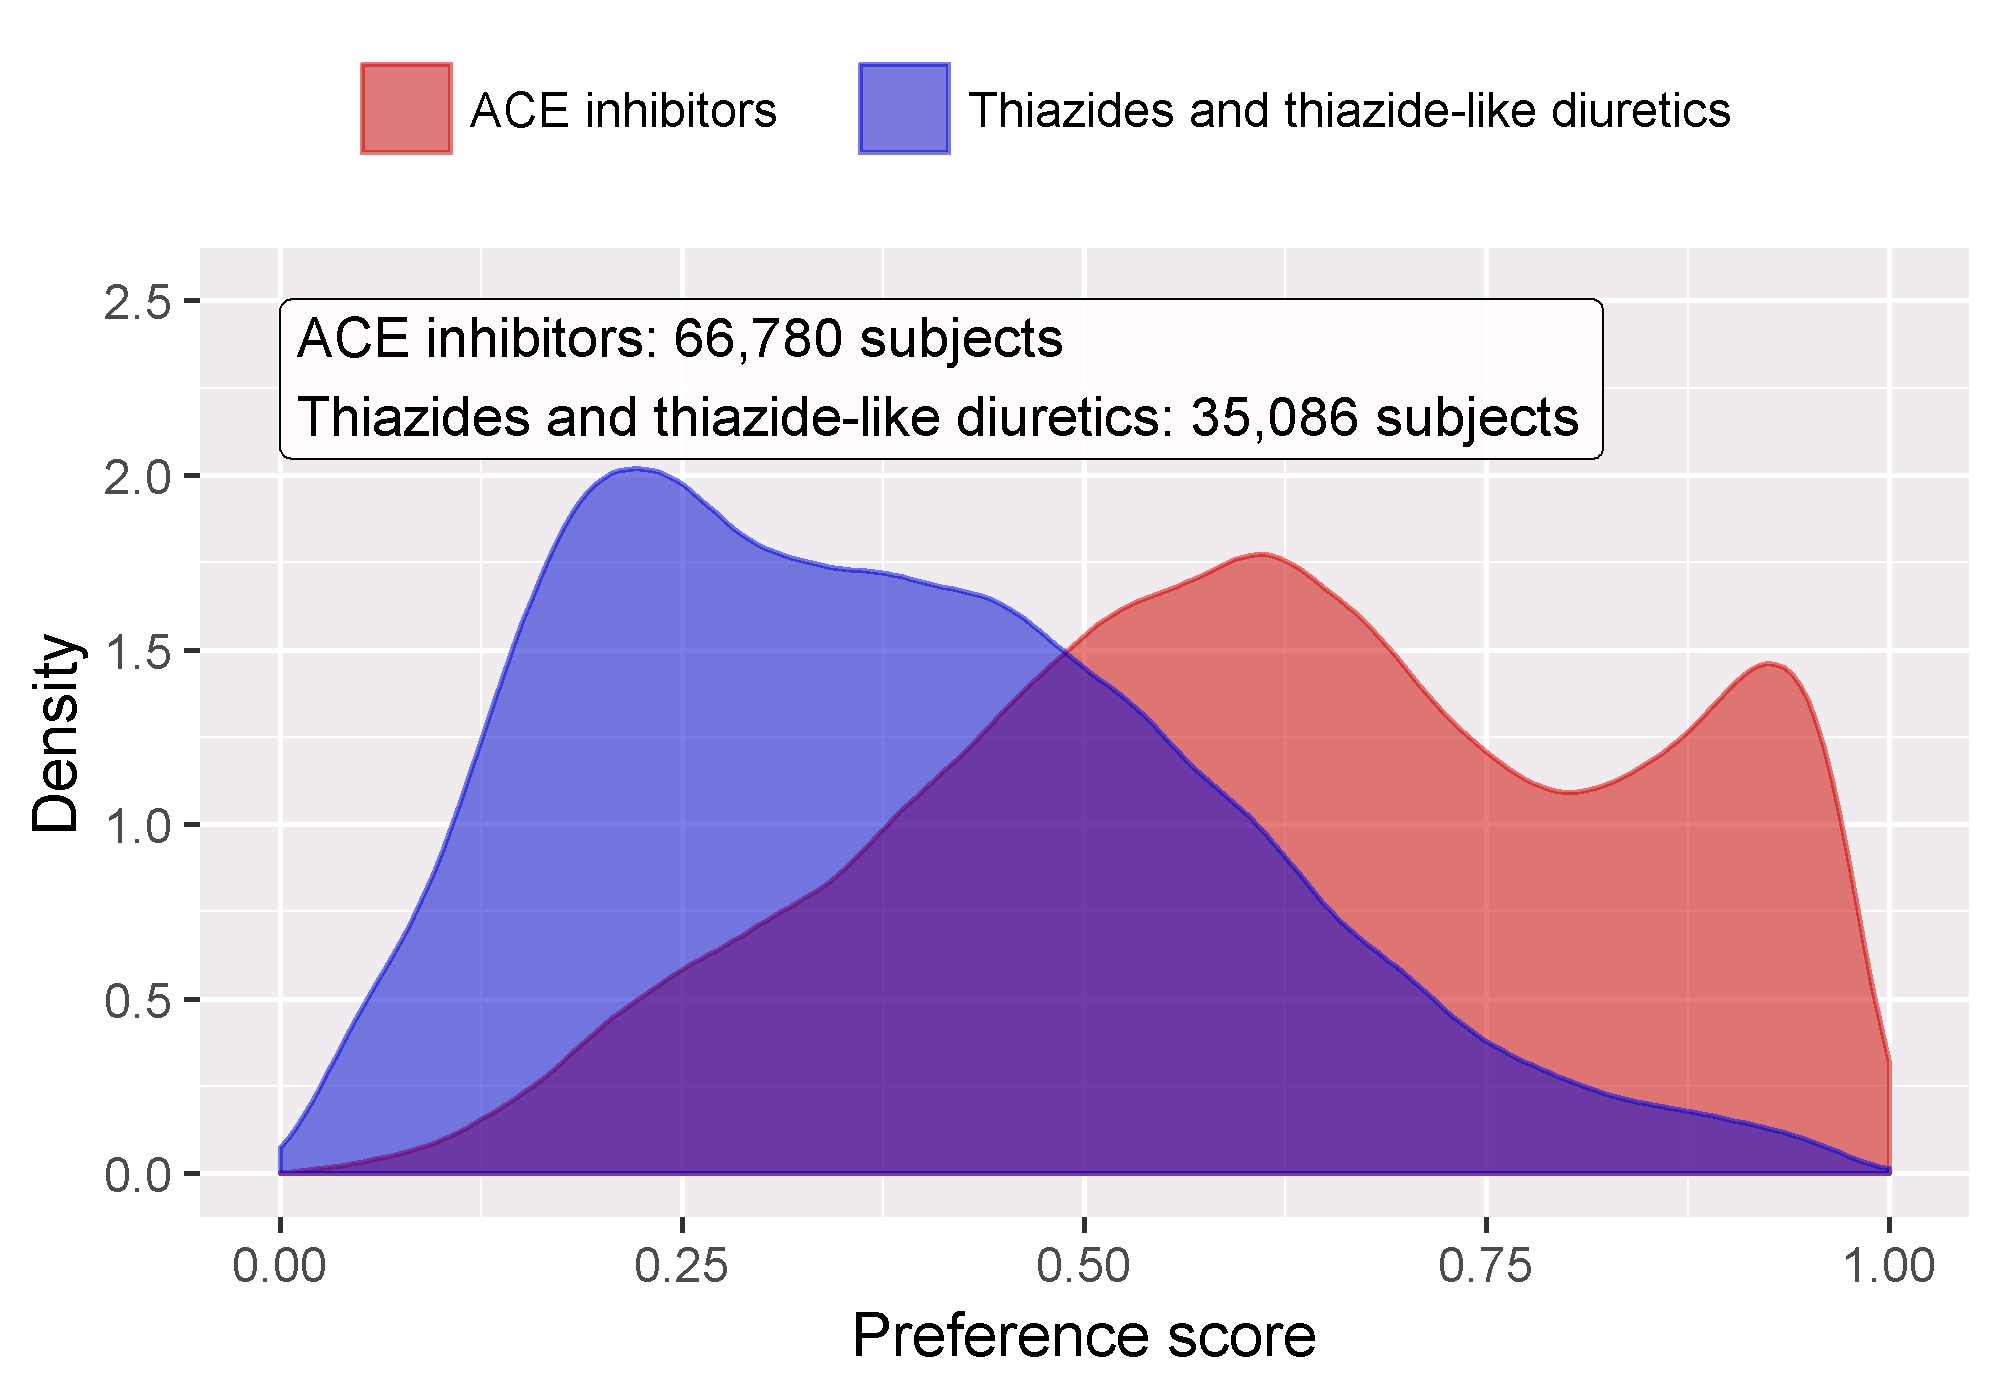
\includegraphics[width=0.8\linewidth]{images/PopulationLevelEstimation/ps} 

}

\caption{Preference score distribution.}\label{fig:ps}
\end{figure}

In general it is a good idea to also inspect the propensity model
itself, and especially so if the model is very predictive. That way we
may discover which variables are most predictive. Table
\ref{tab:psModel} shows the top predictors in our propensity model. Note
that if a variable is too predictive, the CohortMethod package will
throw an informative error rather than attempt to fit a model that is
already known to be perfectly predictive.

\begin{longtable}[]{@{}rl@{}}
\caption{\label{tab:psModel} Top 10 predictors in the propensity model for
ACEi and THZ. Positive values mean subjects with the covariate are more
likely to receive the target treatment.}\tabularnewline
\toprule
\begin{minipage}[b]{0.07\columnwidth}\raggedleft\strut
Beta\strut
\end{minipage} & \begin{minipage}[b]{0.87\columnwidth}\raggedright\strut
Covariate\strut
\end{minipage}\tabularnewline
\midrule
\endfirsthead
\toprule
\begin{minipage}[b]{0.07\columnwidth}\raggedleft\strut
Beta\strut
\end{minipage} & \begin{minipage}[b]{0.87\columnwidth}\raggedright\strut
Covariate\strut
\end{minipage}\tabularnewline
\midrule
\endhead
\begin{minipage}[t]{0.07\columnwidth}\raggedleft\strut
-1.42\strut
\end{minipage} & \begin{minipage}[t]{0.87\columnwidth}\raggedright\strut
condition\_era group during day -30 through 0 days relative to index:
Edema\strut
\end{minipage}\tabularnewline
\begin{minipage}[t]{0.07\columnwidth}\raggedleft\strut
-1.11\strut
\end{minipage} & \begin{minipage}[t]{0.87\columnwidth}\raggedright\strut
drug\_era group during day 0 through 0 days relative to index: Potassium
Chloride\strut
\end{minipage}\tabularnewline
\begin{minipage}[t]{0.07\columnwidth}\raggedleft\strut
0.68\strut
\end{minipage} & \begin{minipage}[t]{0.87\columnwidth}\raggedright\strut
age group: 05-09\strut
\end{minipage}\tabularnewline
\begin{minipage}[t]{0.07\columnwidth}\raggedleft\strut
0.64\strut
\end{minipage} & \begin{minipage}[t]{0.87\columnwidth}\raggedright\strut
measurement during day -365 through 0 days relative to index:
Renin\strut
\end{minipage}\tabularnewline
\begin{minipage}[t]{0.07\columnwidth}\raggedleft\strut
0.63\strut
\end{minipage} & \begin{minipage}[t]{0.87\columnwidth}\raggedright\strut
condition\_era group during day -30 through 0 days relative to index:
Urticaria\strut
\end{minipage}\tabularnewline
\begin{minipage}[t]{0.07\columnwidth}\raggedleft\strut
0.57\strut
\end{minipage} & \begin{minipage}[t]{0.87\columnwidth}\raggedright\strut
condition\_era group during day -30 through 0 days relative to index:
Proteinuria\strut
\end{minipage}\tabularnewline
\begin{minipage}[t]{0.07\columnwidth}\raggedleft\strut
0.55\strut
\end{minipage} & \begin{minipage}[t]{0.87\columnwidth}\raggedright\strut
drug\_era group during day -365 through 0 days relative to index:
INSULINS AND ANALOGUES\strut
\end{minipage}\tabularnewline
\begin{minipage}[t]{0.07\columnwidth}\raggedleft\strut
-0.54\strut
\end{minipage} & \begin{minipage}[t]{0.87\columnwidth}\raggedright\strut
race = Black or African American\strut
\end{minipage}\tabularnewline
\begin{minipage}[t]{0.07\columnwidth}\raggedleft\strut
0.52\strut
\end{minipage} & \begin{minipage}[t]{0.87\columnwidth}\raggedright\strut
(Intercept)\strut
\end{minipage}\tabularnewline
\begin{minipage}[t]{0.07\columnwidth}\raggedleft\strut
0.50\strut
\end{minipage} & \begin{minipage}[t]{0.87\columnwidth}\raggedright\strut
gender = MALE\strut
\end{minipage}\tabularnewline
\bottomrule
\end{longtable}

\BeginKnitrBlock{rmdimportant}
If a variable is found to be highly predictive, there are two possible
conclusions: Either we find that the variable is clearly part of the
exposure itself and should be removed before fitting the model, or else
we must conclude that the two populations are truly incomparable, and
the analysis must be stopped.
\EndKnitrBlock{rmdimportant}

\subsection{Covariate balance}\label{covariate-balance}

The goal of using PS is to make the two groups comparable (or at least
to select comparable groups). We must verify whether this is achieved,
for example by checked whether the baseline covariates are indeed
balanced after adjustment. We can use the
\texttt{computeCovariateBalance} and
\texttt{plotCovariateBalanceScatterPlot} functions to generate Figure
\ref{fig:balance}. One rule-of-thumb to use is that no covariate may
have an absolute standardized difference of means greater than 0.1 after
propensity score adjustment. Here we see that although there was
substantial imbalance before matching, after matching we meet this
criterion.

\begin{figure}

{\centering 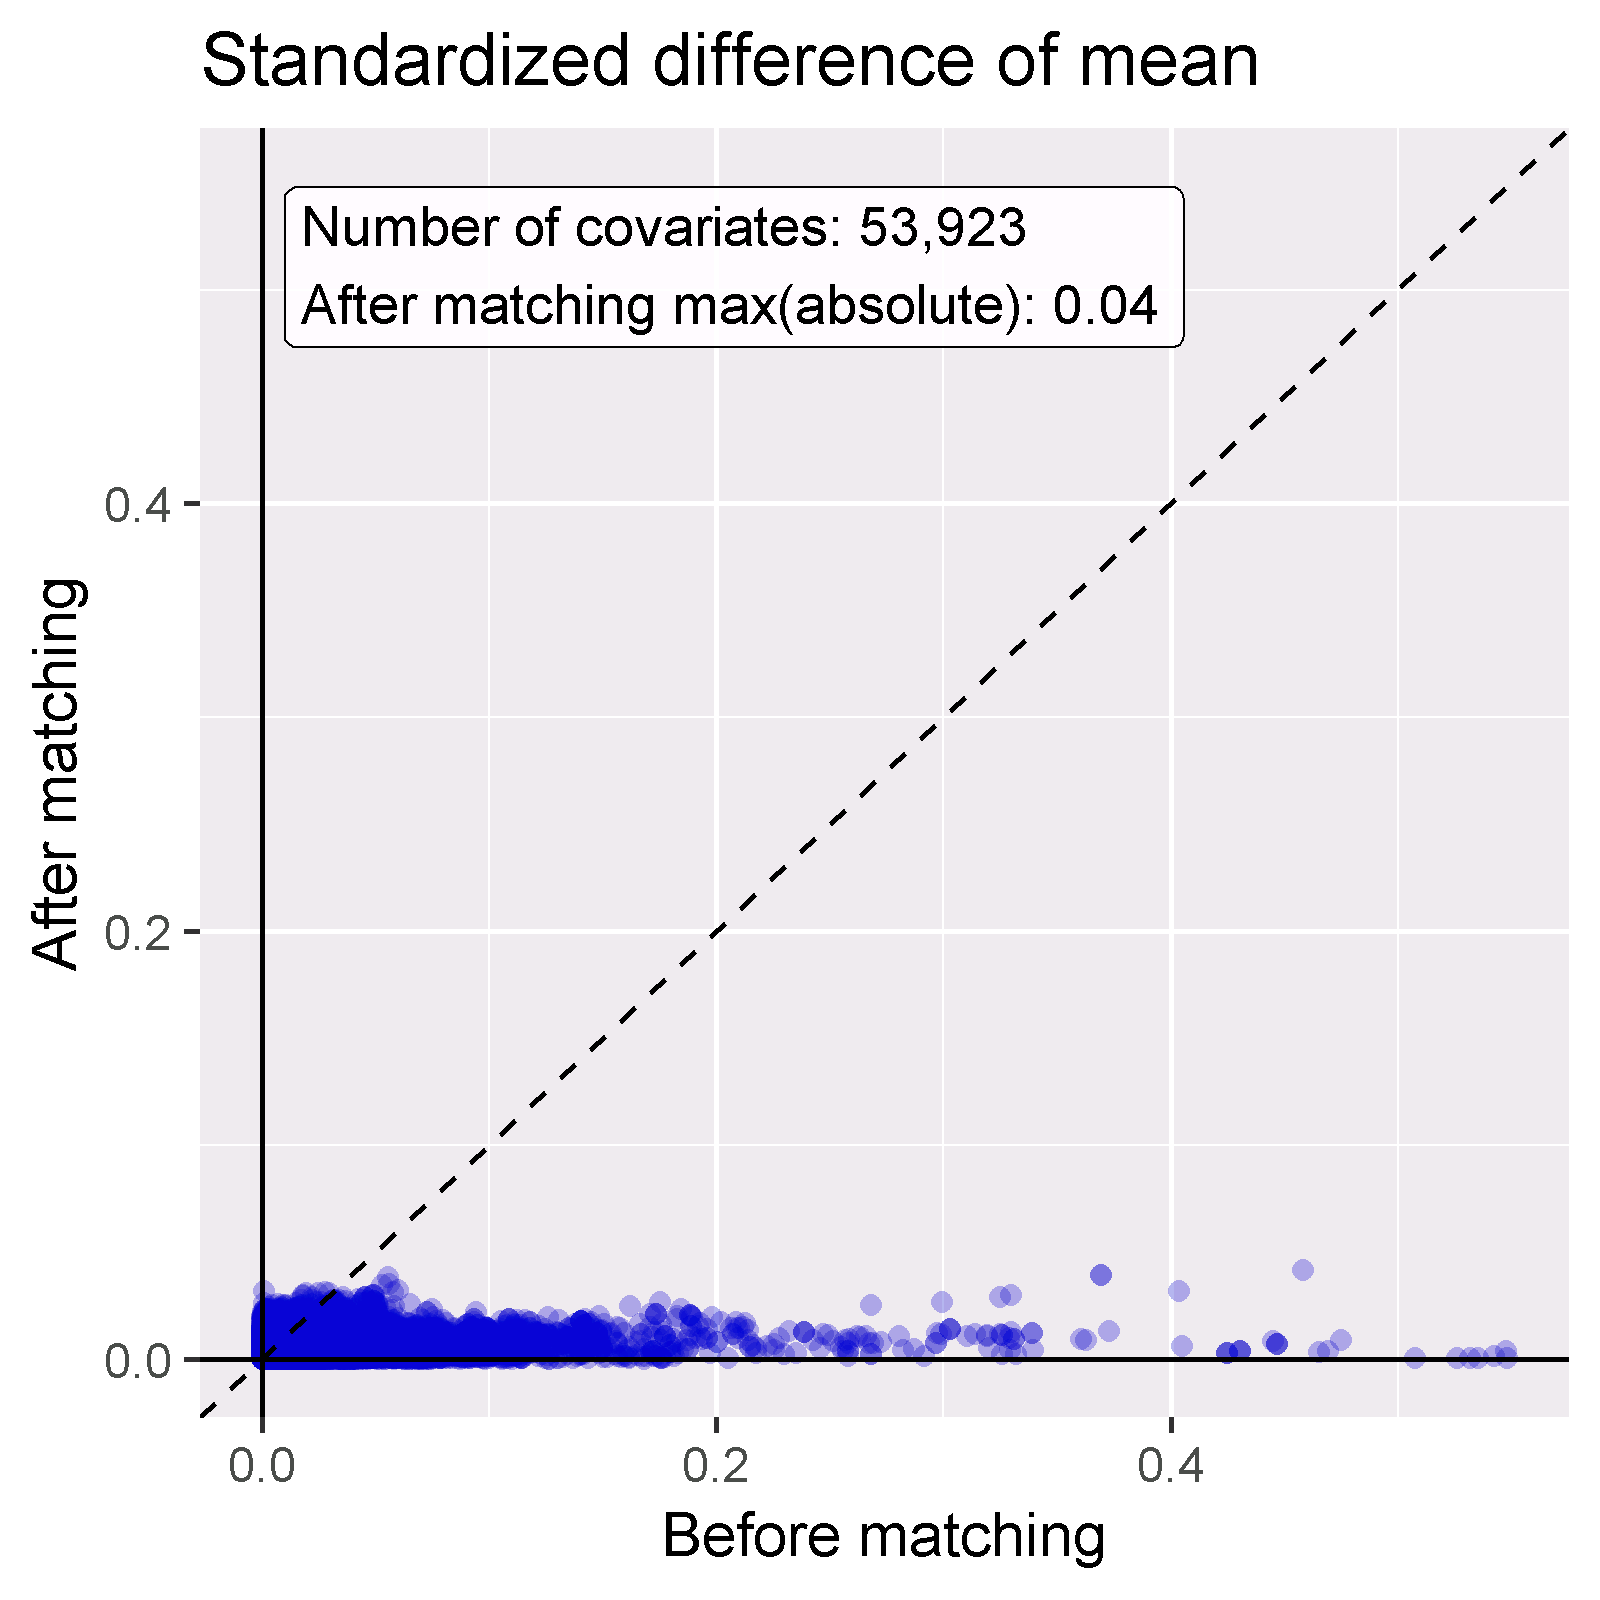
\includegraphics[width=0.7\linewidth]{images/PopulationLevelEstimation/balance} 

}

\caption{Covariate balance, showing the absolute standardized difference of mean before and after propensity score matching. Each blue dot represents a covariate.}\label{fig:balance}
\end{figure}

\subsection{Follow up and power}\label{follow-up-and-power}

Before fitting an outcome model, we might be interested to know whether
we have sufficient power to detect a particular effect size. It makes
sense to perform these power calculations once the study population has
been fully defined, so taking into account loss to the various inclusion
and exclusion criteria (such as no prior outcomes), and loss due to
matching and/or trimming. We can view the attrition of subjects in our
study using the \texttt{drawAttritionDiagram} function as shown in
Figure \ref{fig:attrition}.

\begin{figure}

{\centering 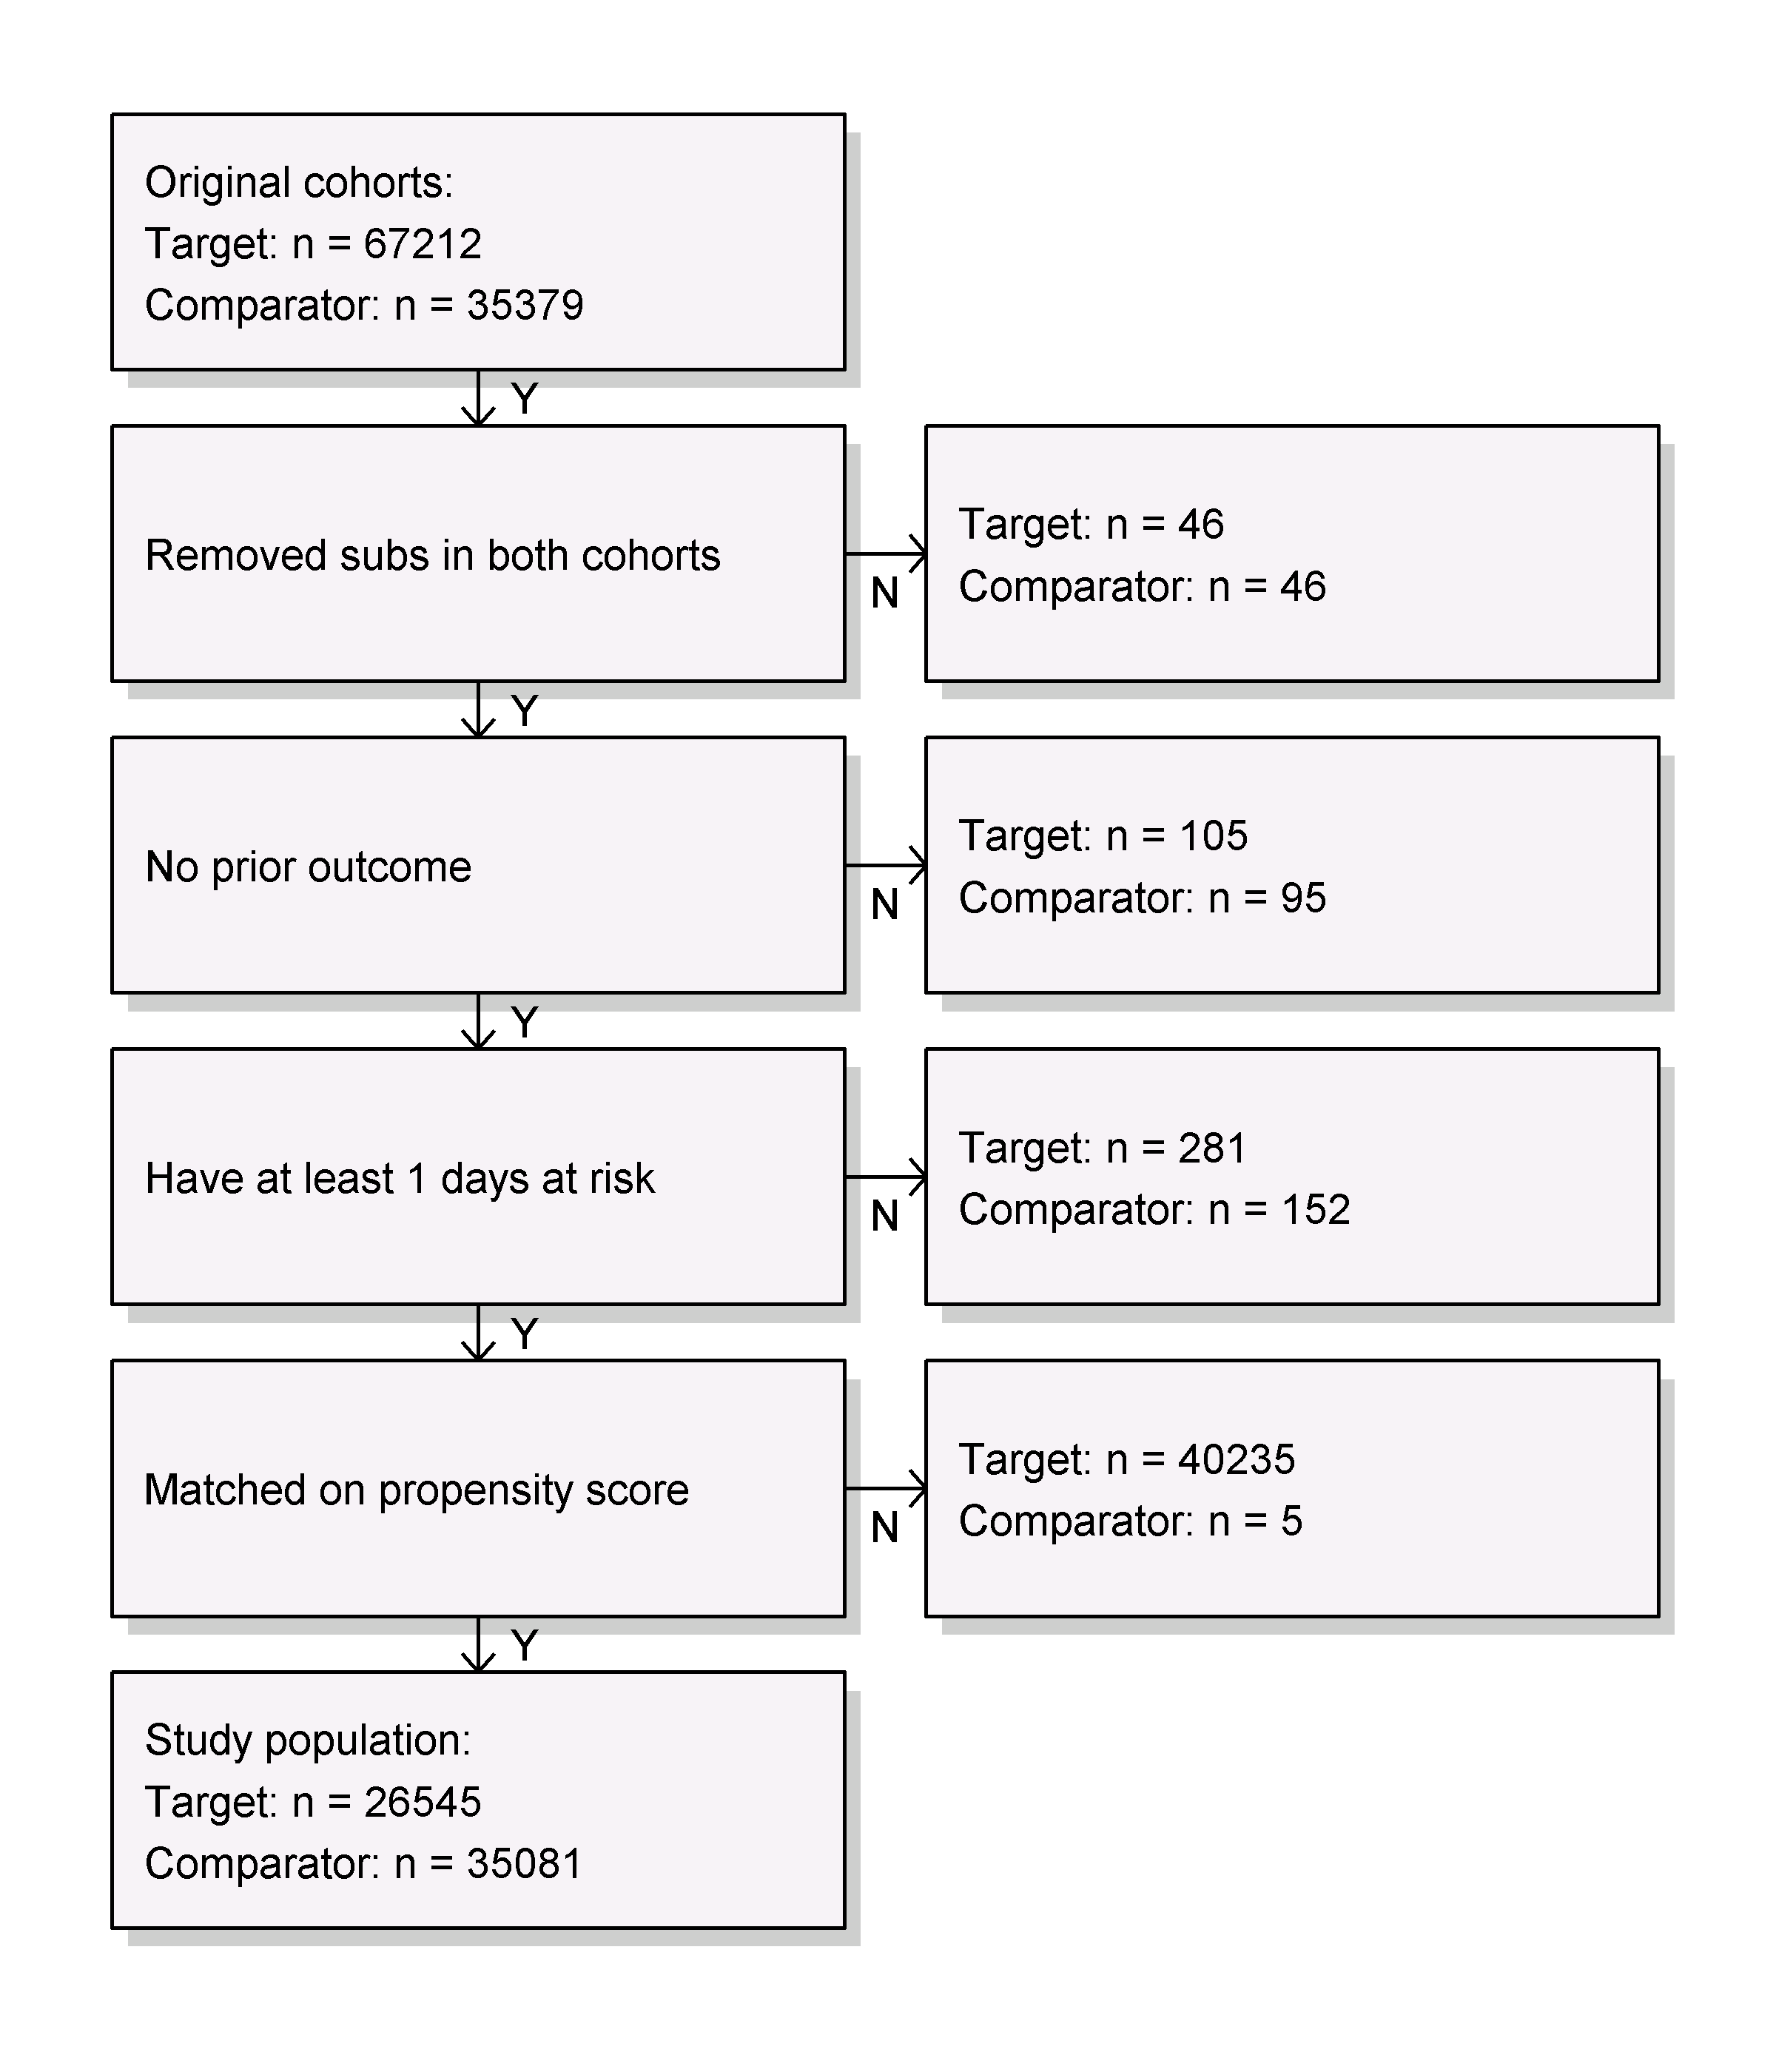
\includegraphics[width=0.7\linewidth]{images/PopulationLevelEstimation/attrition} 

}

\caption{Attrition diagram. The counts shown at the top are those that meet our target and comparator cohort definitions. The counts at the bottom are those that enter our outcome model, in  this case a Cox regression.}\label{fig:attrition}
\end{figure}

Since the sample size is fixed in retrospective studies (the data has
already been collected), and the true effect size is unknown, it is
therefore less meaningful to compute the power given an expected effect
size. Instead, the CohortMethod package provides the
\texttt{computeMdrr} function to compute the minimum detectable relative
risk (MDRR). In our example study the MDRR is 1.69.

To gain a better understanding of the amount of follow-up available we
can also inspect the distribution of follow-up time. We defined
follow-up time as time at risk, so not censored by the occurrence of the
outcome. The \texttt{getFollowUpDistribution} can provide a simple
overview as shown in Figure \ref{fig:followUp}, which suggests the
follow-up time for both cohorts is comparable.

\begin{figure}

{\centering 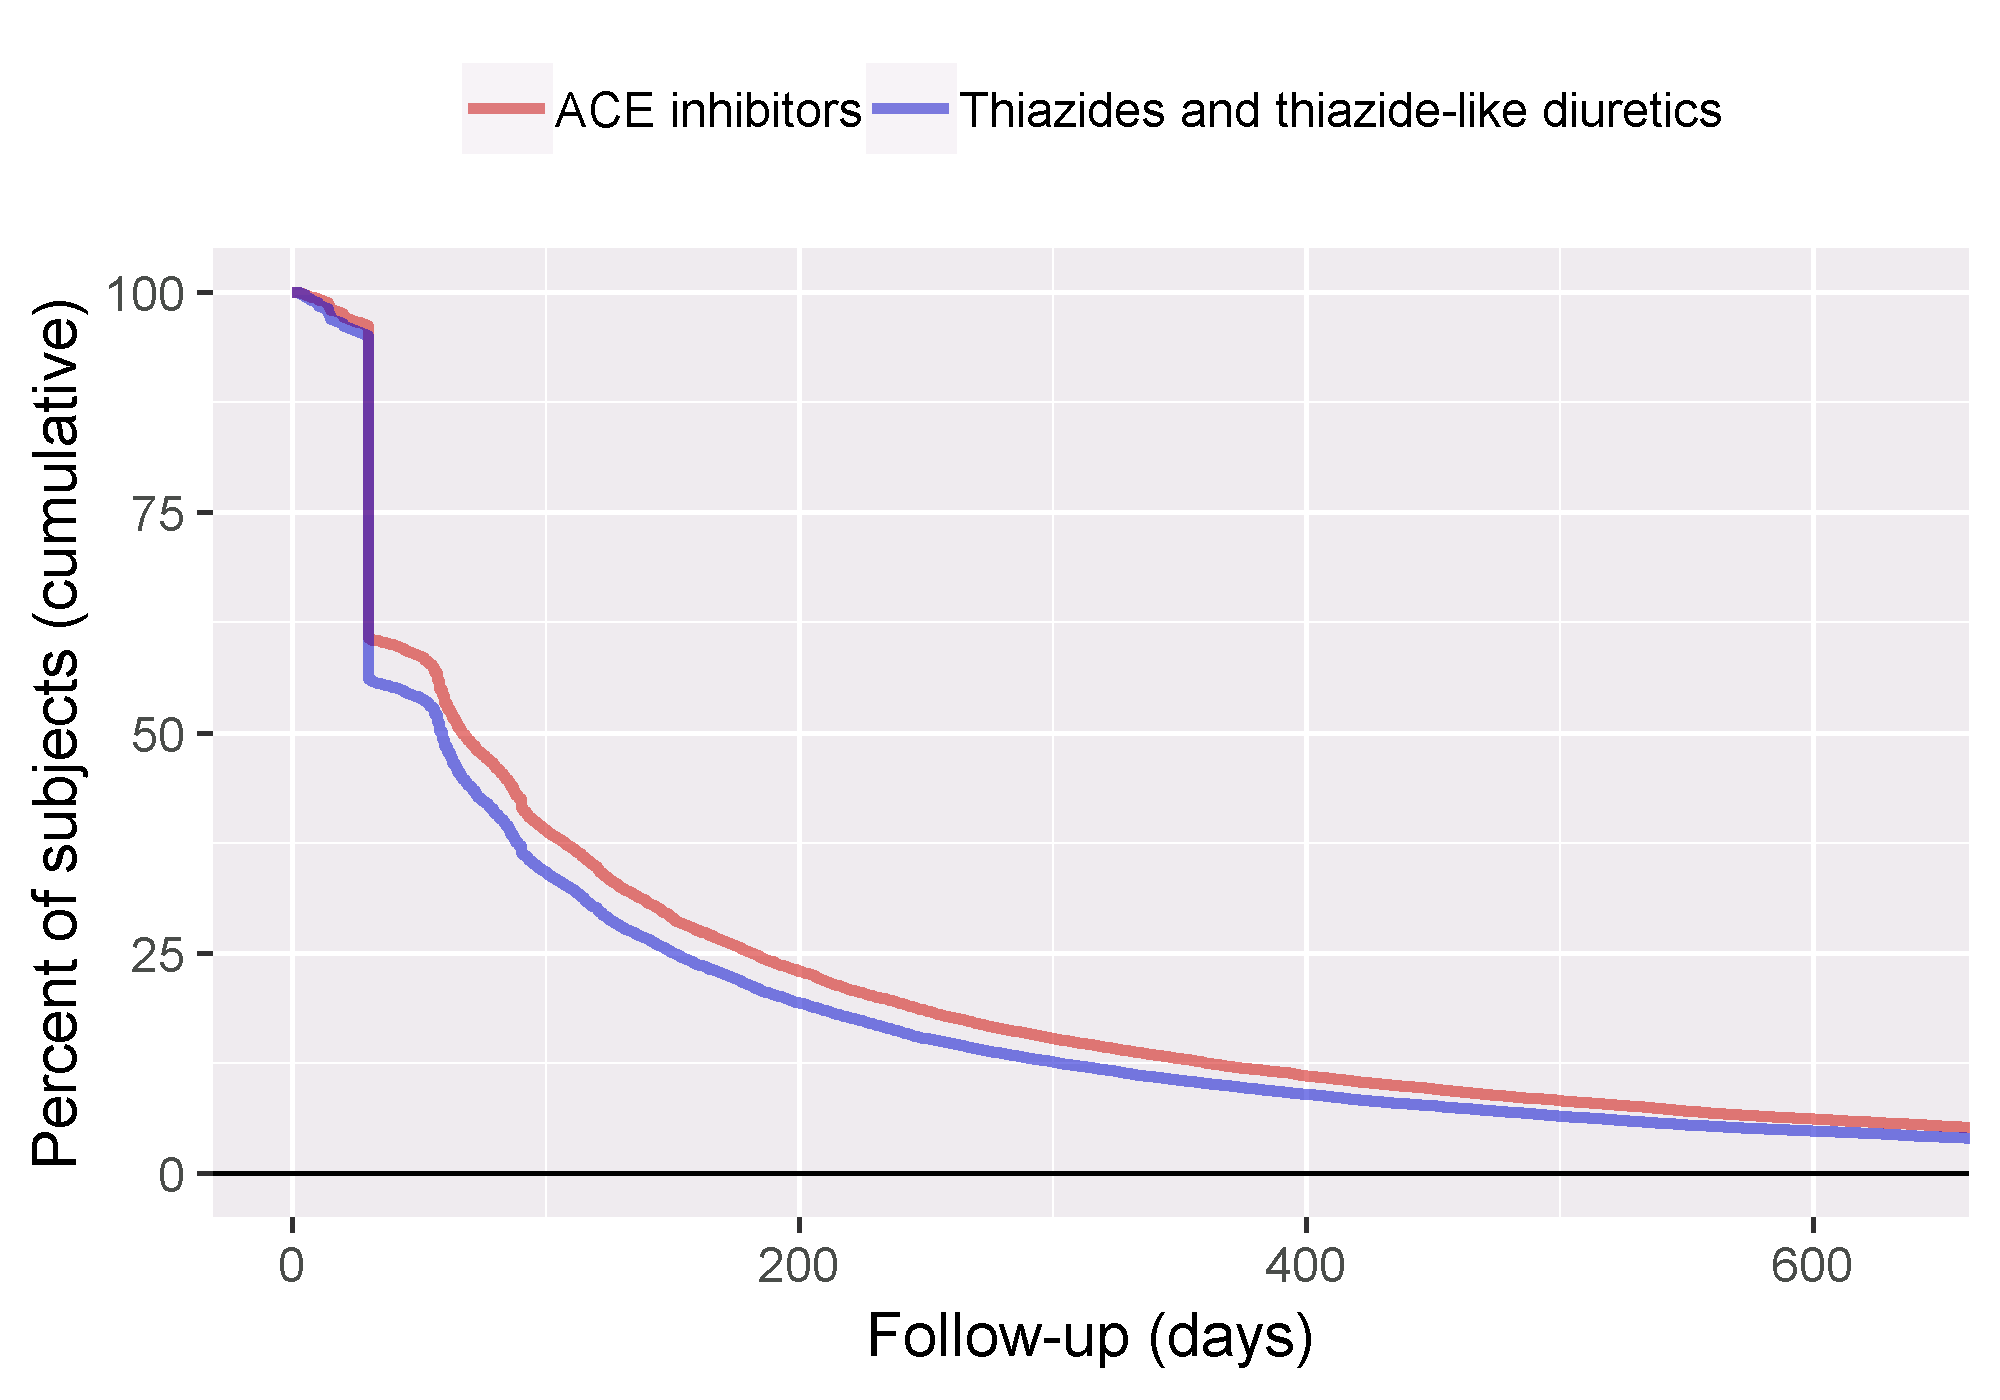
\includegraphics[width=0.8\linewidth]{images/PopulationLevelEstimation/followUp} 

}

\caption{Distribution of follow-up time for the target and comparator cohorts.}\label{fig:followUp}
\end{figure}

\subsection{Kaplan Meier}\label{kaplan-meier}

One last check is to review the Kaplan Meier plot, showing the survival
over time in both cohorts. Using the \texttt{plotKaplanMeier} function
we can create \ref{fig:kmPlot}, which we can check for example if our
assumption of proportionality of hazards holds. The Kaplan-Meier plot
automatically adjusts for stratification or weighting by PS. In this
case, because variable-ratio matching is used, the survival curve for
the comparator groups is adjusted to mimick what the curve had looked
like for the target group had they been exposued to the comparator
instead.

\begin{figure}

{\centering 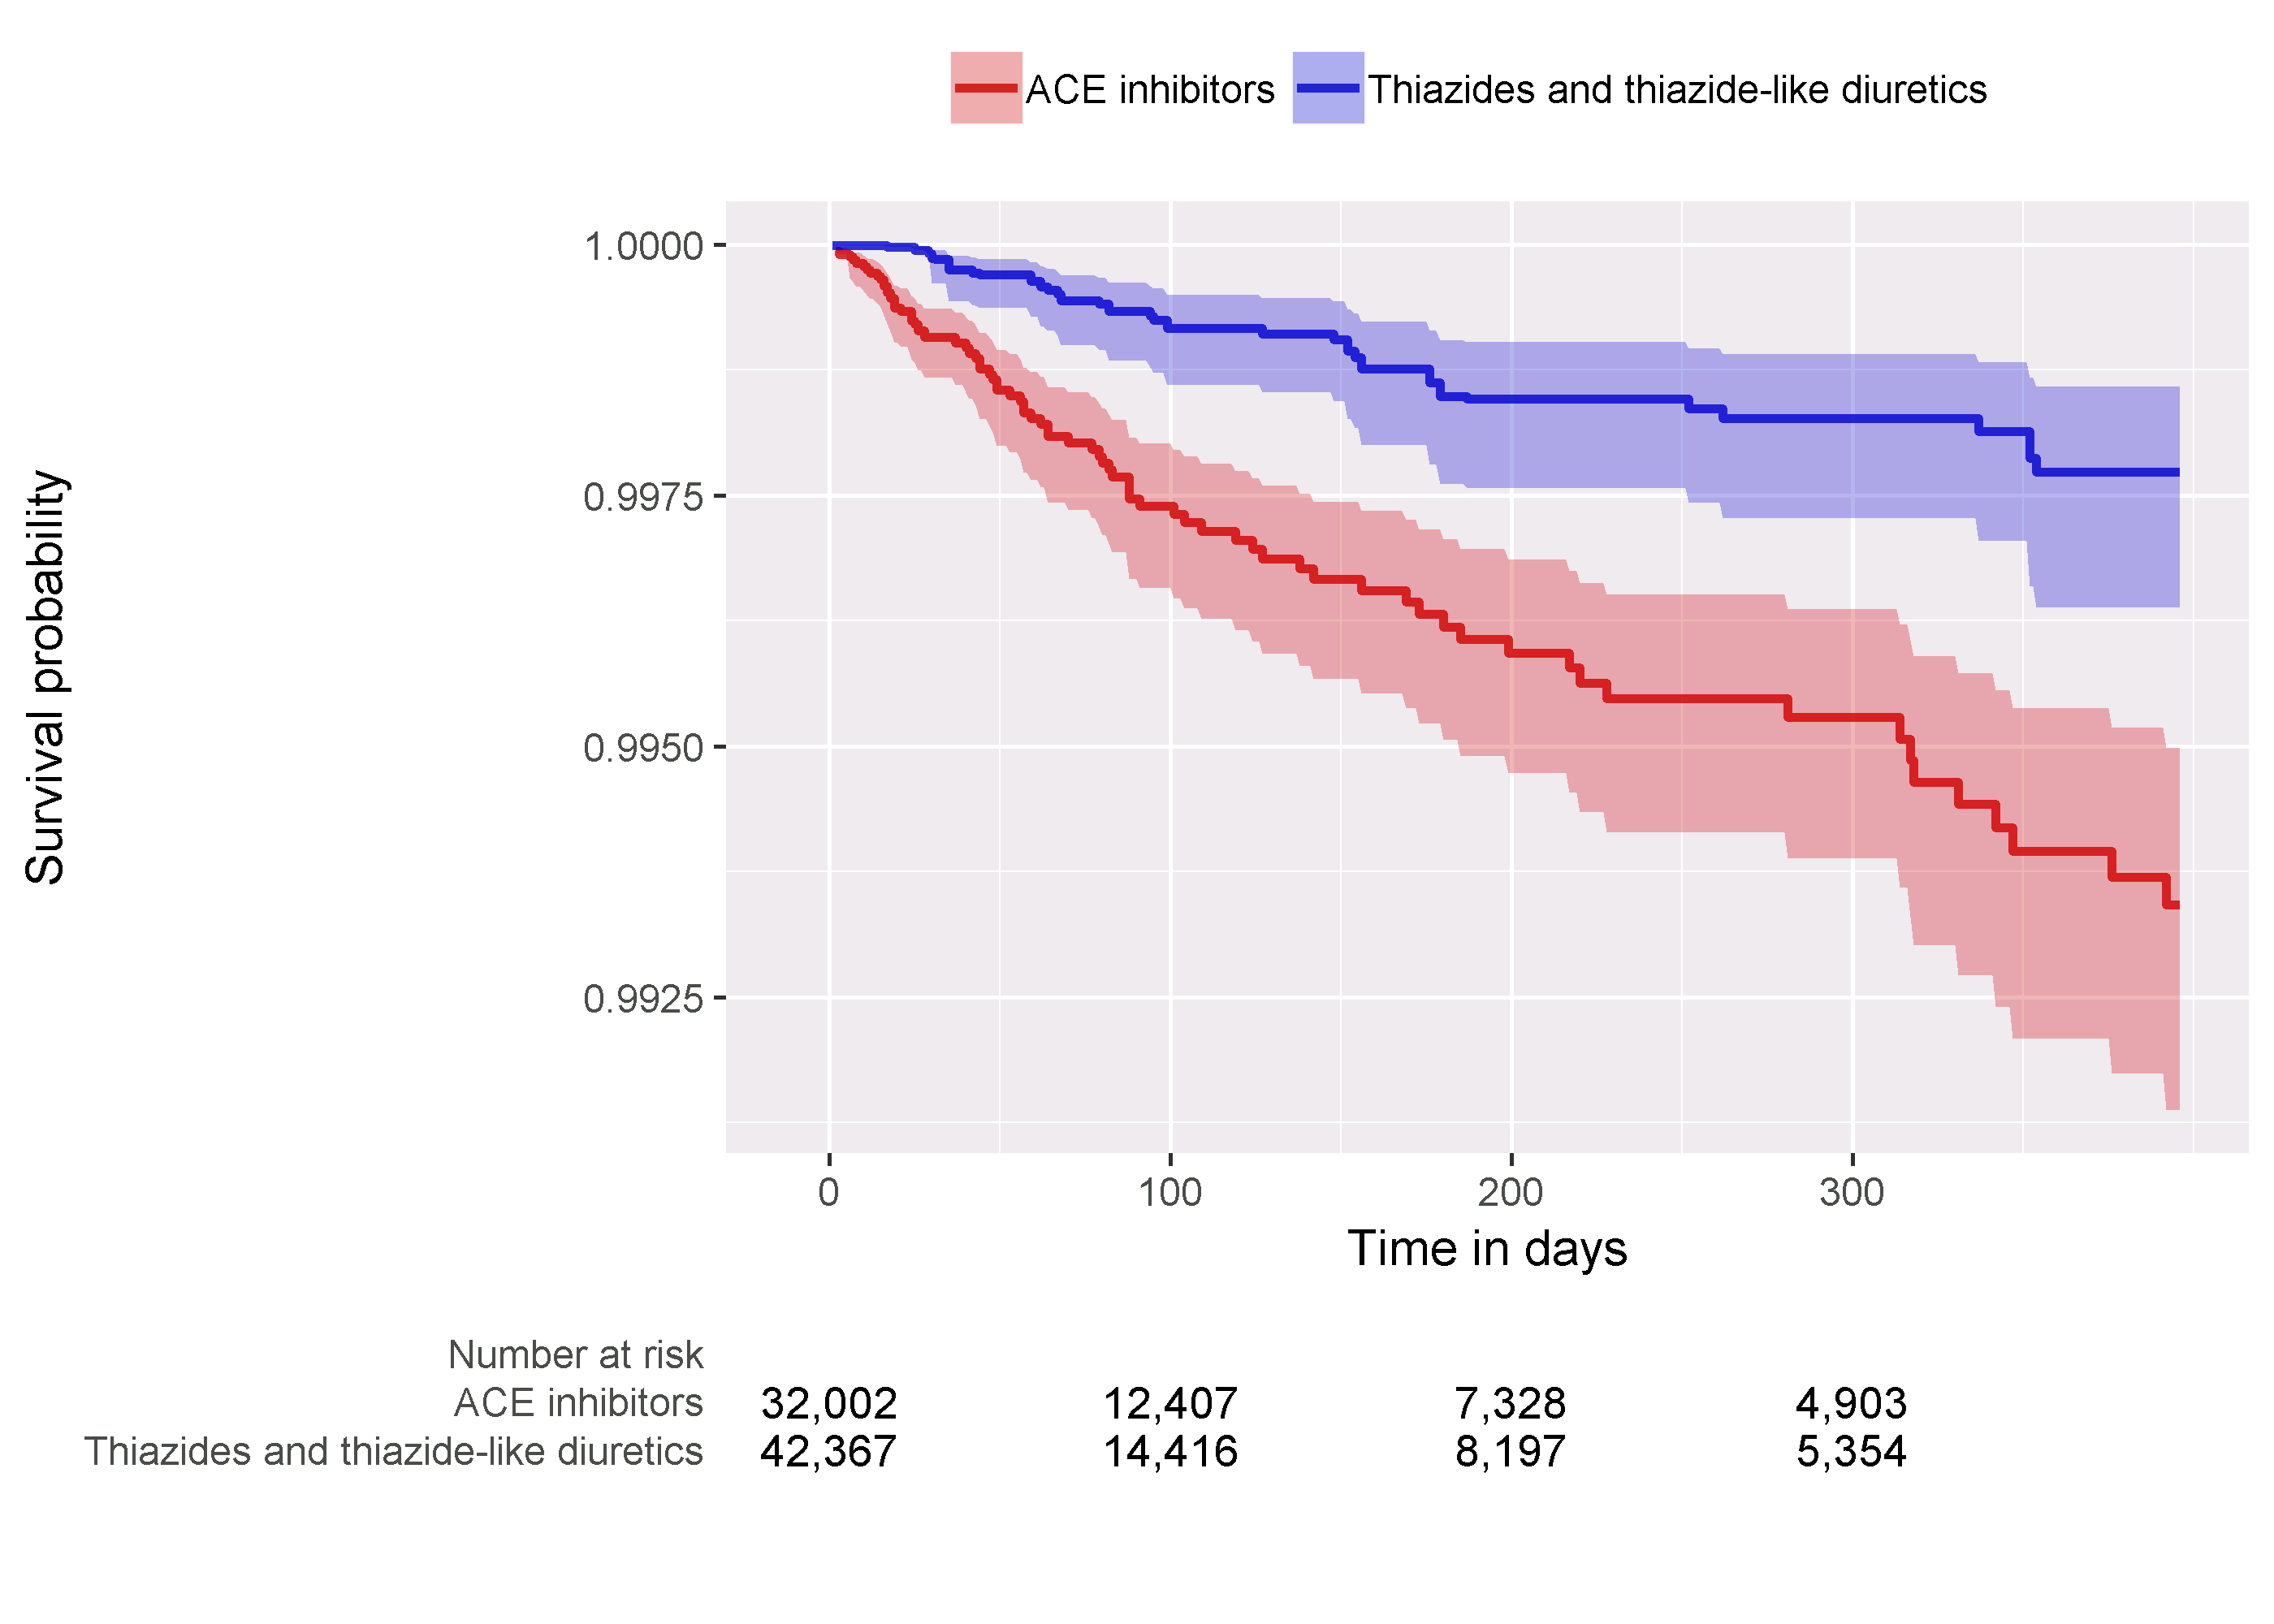
\includegraphics[width=1\linewidth]{images/PopulationLevelEstimation/kmPlot} 

}

\caption{Kaplan Meier plot.}\label{fig:kmPlot}
\end{figure}

\subsection{Effect size estimate}\label{effect-size-estimate}

We observe a hazard ratio of 4.32 (95\% confidence interval: 2.45 -
8.08) for angioedema, which tells us that ACEi appear to increase the
risk of angioedema compared to THZ. Similarly, we observe a hazard ratio
of 1.13 (95\% confidence interval: 0.59 - 2.18) for AMI, suggesting
little or no effect for AMI. Our diagnostics, as reviewed earlier, give
no reason for doubt. However, ultimately the quality of this evidence,
and whether we choose to trust it, depends on many factors that are not
covererd by the study diagnostics as described in Chapter
\ref{EvidenceQuality}.

\section{Summary}\label{summary-3}

\BeginKnitrBlock{rmdsummary}
\begin{itemize}
\item
  Population-level estimation aims to infer causal effects from
  observational data.
\item
  The \textbf{counterfactual}, what would have happened if the subject
  had received an alternative exposure or no exposure, cannot be
  observed.
\item
  Different designs aim to construct the counterfactual in different
  ways.
\item
  The various designs as implemented in the OHDSI Methods Library
  provide diagnostics to evaluate whether the assumptions for creating
  an appropriate counterfactual have been met.
\end{itemize}
\EndKnitrBlock{rmdsummary}

\section{Excercises}\label{excercises}

Note: The excercises still have to be defined. The idea is to require
readers to define a study that estimates the effect of celecoxib on GI
bleed, compared to diclofenac. For this they must use the Eunomia
package, which is still under development.

\chapter{Patient Level Prediction}\label{PatientLevelPrediction}

\emph{Chapter leads: Peter Rijnbeek \& Jenna Reps}

\section{Introduction}\label{introduction}

Clinical decision making is a complicated task in which the clinician
has to infer a diagnosis or treatment pathway based on the available
medical history of the patient and the current clinical guidelines.
Clinical prediction models have been developed to support this decision
making process and are used in clinical practice in a wide spectrum of
specialties. These models predict a diagnostic or prognostic outcome
based on a combination of patient characteristics, e.g.~demographic
information, disease history, treatment history. The number of
publications describing clinical prediction models has increased
strongly over the last 10 years. An example is the Garvan model that
predicts the 5-years and 10-years fractures risk in any elderly man or
woman based on age, fracture history, fall history, bone mass density or
weight \citep{nguyen2008}. Many prediction models have been developed in
patient subgroups at higher risk that need more intensive monitoring,
e.g.~the prediction of 30-day mortality after an acute myocardial
described by \citet{lee1995}. Also, many models have been developed for
asymptomatic subjects in the population, e.g.~the famous Framingham risk
functions for cardiovascular disease \citep{wilson1998}, or the models
for breast cancer screening \citep{engel2015}.

Surprisingly, most currently used models are estimated using small
datasets and contain a limited set of patient characteristics. For
example, in a review of 102 prognostic models in traumatic brain injury
showed that three quarters of the models were based on samples with less
than 500 patients \citep{perel2006}. This low sample size, and thus low
statistical power, forces the data analyst to make stronger modelling
assumptions. The selection of the often limited set of patient
characteristics is strongly guided by the expert knowledge at hand. This
contrasts sharply with the reality of modern medicine wherein patients
generate a rich digital trail, which is well beyond the power of any
medical practitioner to fully assimilate. Presently, health care is
generating huge amount of patient-specific information contained in the
Electronic Health Record (EHR). This includes structured data in the
form of diagnose, medication, laboratory test results, and unstructured
data contained in clinical narratives. Currently, it is unknown how much
predictive accuracy can be gained by leveraging the large amount of data
originating from the complete EHR of a patient.

Massive-scale, patient-specific predictive modeling has become reality
due the OHDSI initiative in which the common data model (CDM) allows for
uniform and transparent analysis at an unprecedented scale. These large
standardized populations contain rich data to build highly predictive
large-scale models and also provide immediate opportunity to serve large
communities of patients who are in most need of improved quality of
care. Such models can inform truly personalized medical care leading
hopefully to sharply improved patient outcomes. Furthermore, these
models could assist in the design and analysis of randomized controlled
trials (RCT) by enabling a better patient stratification or can be
utilized to adjust for confounding variables in observational research.
More accurate prediction models contribute to targeting of treatment and
to increasing cost-effectiveness of medical care.

Advances in machine learning for large dataset analysis have led to
increased interest in applying patient-level prediction on this type of
data. However, many published efforts in patient-level-prediction do not
follow the model development guidelines, fail to perform extensive
external validation, or provide insufficient model details that limits
the ability of independent researchers to reproduce the models and
perform external validation. This makes it hard to fairly evaluate the
predictive performance of the models and reduces the likelihood of the
model being used appropriately in clinical practice. To improve
standards, several papers have been written detailing guidelines for
best practices in developing and reporting prediction models.

The Transparent Reporting of a multivariable prediction model for
Individual Prognosis Or Diagnosis (TRIPOD) statement \footnote{\url{https://www.equator-network.org/reporting-guidelines/tripod-statement/}}
provides clear recommendations for reporting prediction model
development and validation and addresses some of the concerns related to
transparency. However, data structure heterogeneity and inconsistent
terminologies still make collaboration and model sharing difficult as
different researchers are often required to write new code to extract
the data from their databases and may define variables differently.

In our paper \citep{reps2018}, we propose a standardised framework for
patient-level prediction that utilizes the OMOP Common Data Model (CDM)
and standardized vocabularies, and describe the open-source software
that we developed implementing the framework's pipeline. The framework
is the first to support existing best practice guidelines and will
enable open dissemination of models that can be extensively validated
across the network of OHDSI collaborators.

Figure \ref{fig:figure1}, illustrates the prediction problem we address.
Among a population at risk, we aim to predict which patients at a
defined moment in time (t = 0) will experience some outcome during a
time-at-risk. Prediction is done using only information about the
patients in an observation window prior to that moment in time.

\begin{figure}
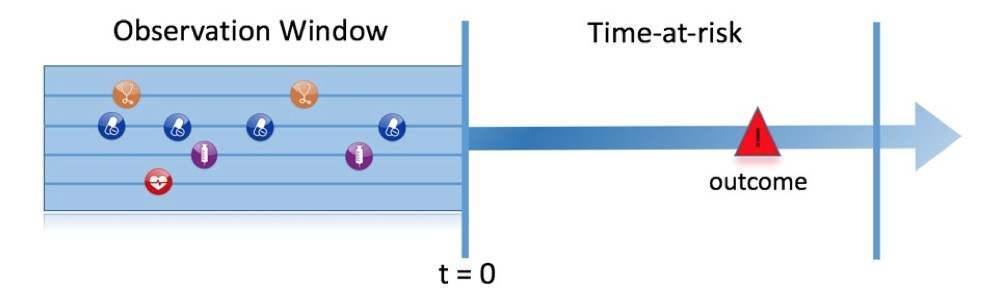
\includegraphics[width=1\linewidth]{images/PatientLevelPrediction/Figure1} \caption{The prediction problem.}\label{fig:figure1}
\end{figure}

As shown in Table \ref{tab:plpDesign}, to define a prediction problem we
have to define t=0 by a target Cohort (T), the outcome we like to
predict by an outcome cohort (O), and the time-at-risk (TAR). We define
the standard prediction question as:

\BeginKnitrBlock{rmdimportant}
Amongst {[}add Target cohort definition{]}, who will go on to have
{[}add outcome definition{]} within {[}add time at risk period{]}
\EndKnitrBlock{rmdimportant}

Furthermore, we have to make design choices for the model we like to
develop, and determine the observational datasets to perform internal
and external validation.

\begin{longtable}[]{@{}ll@{}}
\caption{\label{tab:plpDesign} Main design choices in a prediction
design.}\tabularnewline
\toprule
\begin{minipage}[b]{0.23\columnwidth}\raggedright\strut
Choice\strut
\end{minipage} & \begin{minipage}[b]{0.71\columnwidth}\raggedright\strut
Description\strut
\end{minipage}\tabularnewline
\midrule
\endfirsthead
\toprule
\begin{minipage}[b]{0.23\columnwidth}\raggedright\strut
Choice\strut
\end{minipage} & \begin{minipage}[b]{0.71\columnwidth}\raggedright\strut
Description\strut
\end{minipage}\tabularnewline
\midrule
\endhead
\begin{minipage}[t]{0.23\columnwidth}\raggedright\strut
Target cohort\strut
\end{minipage} & \begin{minipage}[t]{0.71\columnwidth}\raggedright\strut
A cohort for whom we wish to predict\strut
\end{minipage}\tabularnewline
\begin{minipage}[t]{0.23\columnwidth}\raggedright\strut
Outcome cohort\strut
\end{minipage} & \begin{minipage}[t]{0.71\columnwidth}\raggedright\strut
A cohort representing the outcome we wish to predict\strut
\end{minipage}\tabularnewline
\begin{minipage}[t]{0.23\columnwidth}\raggedright\strut
Time-at-risk\strut
\end{minipage} & \begin{minipage}[t]{0.71\columnwidth}\raggedright\strut
For what time relative to t=0 do we want to make the prediction?\strut
\end{minipage}\tabularnewline
\begin{minipage}[t]{0.23\columnwidth}\raggedright\strut
Model\strut
\end{minipage} & \begin{minipage}[t]{0.71\columnwidth}\raggedright\strut
What algorithms using which parameters do we want use, and what
predictor variables do we want to include?\strut
\end{minipage}\tabularnewline
\bottomrule
\end{longtable}

This conceptual framework works for all type of prediction problems:

\begin{itemize}
\tightlist
\item
  Disease onset and progression

  \begin{itemize}
  \tightlist
  \item
    \textbf{Structure}: Amongst patients who are newly diagnosed with
    \emph{{[}a disease{]}}, who will go on to have \emph{{[}another
    disease or complication{]}} within \emph{{[}time horizon from
    diagnosis{]}}?
  \item
    \textbf{Example}: Among newly diagnosed atrial fibrilation patients,
    who will go on to have ischemic stroke in the next three years?
  \end{itemize}
\item
  Treatment choice

  \begin{itemize}
  \tightlist
  \item
    \textbf{Structure}: Amongst patients with \emph{{[}indicated
    disease{]}} who are treated with either \emph{{[}treatment 1{]}} or
    \emph{{[}treatment 2{]}}, which patients were treated with
    \emph{{[}treatment 1{]}} (on day 0).
  \item
    \textbf{Example}: Among patients with atrial fibrilation who took
    either warfarin or rivaroxaban, which patients gets warfarin?
    (e.g.~for a propensity model)
  \end{itemize}
\item
  Treatment response

  \begin{itemize}
  \tightlist
  \item
    \textbf{Structure}: Amongst new users of \emph{{[}a treatment{]}},
    who will experience \emph{{[}some effect{]}} in \emph{{[}time
    window{]}} ?
  \item
    \textbf{Example}: Which patients with diabetes who start on
    metformin stay on metform for three years?
  \end{itemize}
\item
  Treatment safety

  \begin{itemize}
  \tightlist
  \item
    \textbf{Structure}: Amongst new users of \emph{{[}a treatment{]}},
    who will experience \emph{{[}adverse event{]}} in \emph{{[}time
    window{]}}?
  \item
    \textbf{Example}: Amongst new users of warfarin, who will have a GI
    bleed in one year?
  \end{itemize}
\item
  Treatment adherence

  \begin{itemize}
  \tightlist
  \item
    \textbf{Structure}: Amongst new users of \emph{{[}a treatment{]}},
    who will achieve \emph{{[}adherence metric{]}} at \emph{{[}time
    window{]}}?
  \item
    \textbf{Example}: Which patients with diabetes who start on
    metformin achieve \textgreater{}=80\% proportion of days covered at
    one year?
  \end{itemize}
\end{itemize}

In the next sections we will explain the best practices for model
specification, implementation, and evaluation using OHDSI's
Patient-Level Prediction (PLP) framework as guidance.

\newpage

\section{Patient-level Prediction
Theory}\label{patient-level-prediction-theory}

\subsection{Creating Labelled Data}\label{creating-labelled-data}

The observational datasets we use in OHDSI consist of timestamped
records of patient medical interactions. These are represented by tables
containing anonymised patient details such as gender and year of birth
in addition to tables containing date stamped medical records.

\begin{figure}
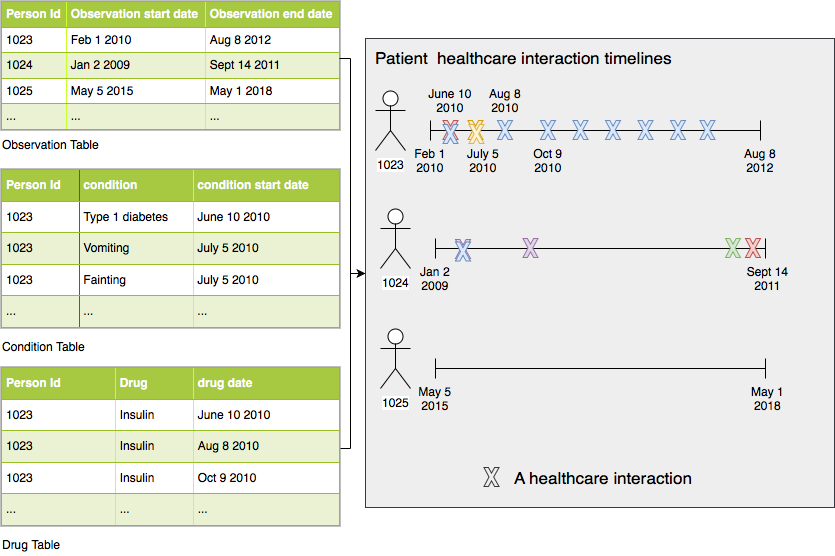
\includegraphics[width=1\linewidth]{images/PatientLevelPrediction/theory/patienttimeline} \caption{Observational data.}\label{fig:figuretheory1}
\end{figure}

Applying supervised learning techniques for prediction requires having
covariate and label pairs for a sufficient number of patients. The
covariates (also referred to as features or independant variables)
describe a patient. Example covariates could be: the patient's gender,
age and health state based on the presence or absense of medical
conditions. Many of these covariates are time dependant, for example age
changes over time, as do some medical conditions. The labels correspond
to whether a patient has a outcome of interest during some time
interval. The label is also time dependant.

To convert the observational data into labelled data consisting of
covariate and label pairs for a set of patients, we need to specify a
point in time for each patient that will be used as a pivot. Covariates
can be constructed at that pivot point in time (using all records up to
that point), and we can can determine whether a patient has the outcome
of interest during some time interval relative to the pivot point in
time (the time at risk).

\begin{figure}
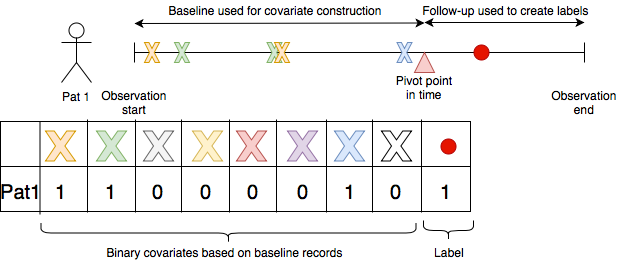
\includegraphics[width=1\linewidth]{images/PatientLevelPrediction/theory/dataplot1} \caption{Create laelled data from observational data.}\label{fig:figuretheory2}
\end{figure}

This will then provide us with labelled data. The definition of the
target cohort population is what we use to define this pivot point in
time. For example, if the target cohort was new users of drug A, then
the pivot point in time is the date a patient first had drug A recorded
in the database. Alternatively, if the target cohort was diagnoses of
cardiovascular disease, then the pivot point in time is the date a
patient first has a record indicating cardiovascular disease is present.
Our prediction specification directly links to how the labelled data are
constructed.

\begin{figure}
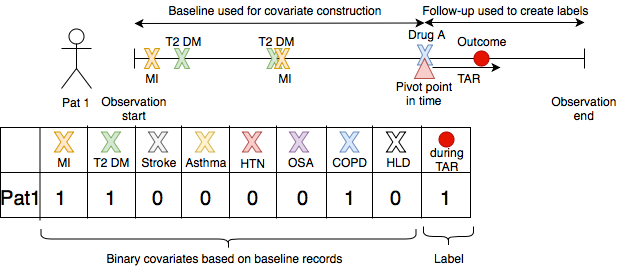
\includegraphics[width=1\linewidth]{images/PatientLevelPrediction/theory/dataplot2} \caption{Create laelled data from observational data.}\label{fig:figuretheory3}
\end{figure}

\subsection{Supervised learning}\label{supervised-learning}

The idea of supervised learning is to be able to generalise what is
observed in the labelled data so that when a new patient's covariates
are known but their label is unknown, we can predict their label.

If we consider the situation where we have two covariates, then we can
represent each patient as a plot in two dimensional space. The
shape/color of a data points corresponds to the patient's label. The
idea of supervised learning is to generalise the what we see and fill in
where there are no current data points. A supervised learning model will
try to partition the space via a decision boundary, as seen in Figure
\ref{fig:figuretheory4} that aims to minimise the cases where the data
point labels do not match the models prediction. Different supervised
learning techniques lead to different decision boundaries and there are
often hyper-parameters that can impact the complexity of the decision
boundary.

\begin{figure}
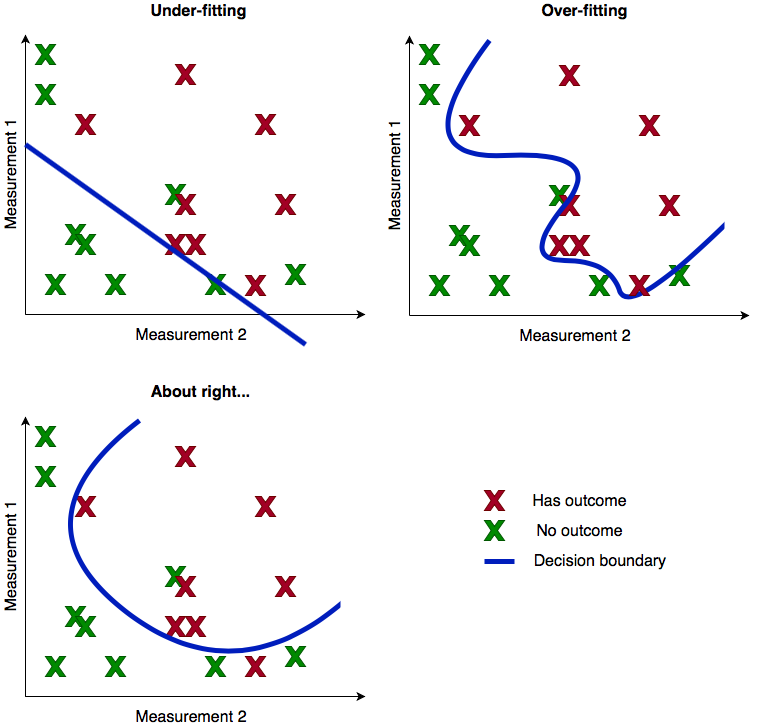
\includegraphics[width=1\linewidth]{images/PatientLevelPrediction/theory/learning} \caption{Decision boundary.}\label{fig:figuretheory4}
\end{figure}

In Figure Figure \ref{fig:figuretheory4} you can see three different
decision boundaries. The boundaries are used to infer the class of any
new data point. In figure Figure \ref{fig:figuretheory5} the decision
boundaries are used to shade the 2 dimentional space into red regions
and green regions. If a new data point falls into the green shaded area
then the model will predict `no outcome', otherwise it will predict `has
outcome'.

Ideally a decision boundary should partition the two classes with no
error. However, generlizability is an issue, as complex models can
`overfit' where they can correctly partition each data points in the
labelled data by using very complex boundaries:

\begin{figure}
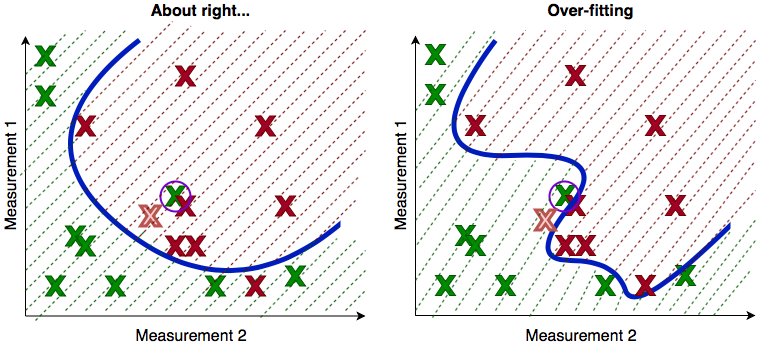
\includegraphics[width=1\linewidth]{images/PatientLevelPrediction/theory/noise} \caption{Overfitting issues.}\label{fig:figuretheory5}
\end{figure}

The issue here is that these boundaries may be fit too closely to the
labelled data used to learn them and may not work for new data. For
example, noise causing incorrectly positioned data points can cause
issues. This is shown in Figure Figure \ref{fig:figuretheory5} where the
decision boundary goes around a data point that was incorrectly
positioned due to noise and this impacts predictions near this region.

Therefore, you want a model that appears to partition the labelled data
well but is also as simple as possible. Techniques such as
regularization aim to maximise model performance on the labelled data
while minimising complexity. Complexity can also be controlled by
picking classifier hyper-parameters such that a simpler decision
boundary is used.

Another way to think about supervised learning is finding a function
that maps from a patient's covariates to their label. {[}add
function{]}. Each supervised learning model has a different way to learn
the mapping function and the no free lunch theorem states that no one
algorithm is always going to outperform the others. The performance of
each type of supervised learning algorithm depends on how the labelled
data points are distributed in space. Therefore we recommend trying
multiple supervised learning techniques when developing patient-level
prediction models.

\subsubsection{Regularized Logistic
Regression}\label{regularized-logistic-regression}

Lasso logistic regression belongs to the family of generalized linear
models, where a linear combination of the variables is learned and
finally a logistic function maps the linear combination to a value
between 0 and 1. The lasso regularization adds a cost based on model
complexity to the objective function when training the model. This cost
is the sum of the absolute values of the linear combination of the
coefficients. The model automatically performs feature selection by
minimizing this cost. We use the
\href{https://ohdsi.github.io/Cyclops/}{Cyclops} (Cyclic coordinate
descent for logistic, Poisson and survival analysis) package to perform
large-scale regularized logistic regression. \textbf{Hyper-parameters}:
var (starting variance), seed.

\subsubsection{Gradient boosting
machines}\label{gradient-boosting-machines}

Gradient boosting machines is a boosting ensemble technique and in our
framework it combines multiple decision trees. Boosting works by
iteratively adding decision trees but adds more weight to the
data-points that are misclassified by prior decision trees in the cost
function when training the next tree. We use Extreme Gradient Boosting,
which is an efficient implementation of the gradient boosting framework
implemented in the xgboost R package available from CRAN.
\textbf{Hyper-parameters}: ntree (number of trees), max depth (max
levels in tree), min rows (minimum data points in in node), learning
rate, seed \textbar{} mtry (number of features in each tree),ntree
(number of trees), maxDepth (max levels in tree), minRows (minimum data
points in in node),balance (balance class labels), seed.

\subsubsection{Random forest}\label{random-forest}

Random forest is a bagging ensemble technique that combines multiple
decision trees. The idea behind bagging is to reduce the likelihood of
overfitting, by using weak classifiers, but combining multiple diverse
weak classifiers into a strong classifier. Random forest accomplishes
this by training multiple decision trees but only using a subset of the
variables in each tree and the subset of variables differ between trees.
Our packages uses the sklearn learn implementation of Random Forest in
python. \textbf{Hyper-parameters}: mtry (number of features in each
tree),ntree (number of trees), maxDepth (max levels in tree), minRows
(minimum data points in in node),balance (balance class labels), seed.

\subsubsection{K-nearest neighbors}\label{k-nearest-neighbors}

K-nearest neighbors (KNN) is an algorithm that uses some metric to find
the K closest labelled data-points, given the specified metric, to a new
unlabelled data-point. The prediction of the new data-points is then the
most prevalent class of the K-nearest labelled data-points. There is a
sharing limitation of KNN, as the model requires labelled data to
perform the prediction on new data, and it is often not possible to
share this data across data sites. We included the
\href{https://github.com/OHDSI/BigKnn}{BigKnn} package developed in
OHDSI which is a large scale k-nearest neighbor classifier.
\textbf{Hyper-parameters}: k (number of neighbours), weighted (weight by
inverse frequency).

\subsubsection{Naive Bayes}\label{naive-bayes}

The Naive Bayes algorithm applies the Bayes theorem with the naive
assumption of conditional independence between every pair of features
given the value of the class variable. Based on the likelihood the data
belongs to a class and the prior distribution of the class, a posterior
distribution is obtained. \textbf{Hyper-parameters}: none.

\subsubsection{AdaBoost}\label{adaboost}

AdaBoost is a boosting ensemble technique. Boosting works by iteratively
adding classifiers but adds more weight to the data-points that are
misclassified by prior classifiers in the cost function when training
the next classifier. We use the sklearn AdaboostClassifier
implementation in Python. \textbf{Hyper-parameters}: nEstimators (the
maximum number of estimators at which boosting is terminated),
learningRate (learning rate shrinks the contribution of each classifier
by learning\_rate. There is a trade-off between learningRate and
nEstimators).

\subsubsection{Decision Tree}\label{decision-tree}

A decision tree is a classifier that partitions the variable space using
individual tests selected using a greedy approach. It aims to find
partitions that have the highest information gain to separate the
classes. The decision tree can easily overfit by enabling a large number
of partitions (tree depth) and often needs some regularization (e.g.,
pruning or specifying hyper-parameters that limit the complexity of the
model). We use the sklearn DecisionTreeClassifier implementation in
Python. \textbf{Hyper-parameters}: maxDepth (the maximum depth of the
tree), minSamplesSplit,minSamplesLeaf, minImpuritySplit (threshold for
early stopping in tree growth. A node will split if its impurity is
above the threshold, otherwise it is a leaf.), seed,classWeight
(``Balance''" or ``None'').

\subsubsection{Multilayer Perception}\label{multilayer-perception}

Neural networks containing multiple layers that weight their inputs
using a non-linear function. The first layer is the input layer, the
last layer is the output layer the between are the hidden layers. Neural
networks are generally trained using feed forward back-propagation. This
is when you go through the network with a data-point and calculate the
error between the true label and predicted label, then go backwards
through the network and update the linear function weights based on the
error. \textbf{Hyper-parameters}: size (the number of hidden nodes),
alpha (the l2 regularisation), seed.

\subsubsection{Deep Learning}\label{deep-learning}

Deep learning such as deep nets, convolutional neural networks or
recurrent neural networks are similar to a neural network but have
multiple hidden layers that aim to learn latent representations useful
for prediction. In a seperate vignette in the
\href{https://ohdsi.github.io/PatientLevelPrediction/}{PatientLevelPrediction}
package we describe these models and hyper-parameters in more detail.

\subsection{Evaluating Models}\label{evaluating-models}

\subsubsection{Evaluation Types}\label{evaluation-types}

There are various ways to evaluate a prediction model: internal
validation, external valdiation, temporal validation and spatial
validation.

Internal validation is when a prediction model is evaluated using the
same dataset used to develop the model. There are three ways to perform
internal validation: using a holdout set, using cross validation and
using bootstrapping. In the patient-level prediction framework we use a
holdout set for internal validation.

A holdout set approach simply splits the labelled data into two
independent sets, a train set and a test set (the hold out set). The
train set is used to learn the model and the test set is used to
evaluate it.

Cross validation is useful when the data are limited. A user needs to
specify the number of folds, such as 10, then the data are split into
that number of independent sets. For each data split, a model is trained
on all other data splits and then applied to the split to obtain the
predicted risks for each patient in the split. The model performance can
then be estimated using the predicted risk obtained when the patients
were held out from model training. A form of cross validation is leave
one out validation, where for each patient, the model is trained using
all other data except that patient's data and then applied to the
patient to obtain their predicted risk. This is repeated for each
patient to obtain risks for all the patients which can be used to
evaluate the model. In the patient-level prediction framework we use
cross validation to pick the optimal hyper-parameters on the train set.

Bootstrapping is useful when calculating confidence intervals. In
bootstrapping multiple sample sets are drawn with replacement from the
whole labelled dataset to generate hold out sets, the unsampled patient
data are used to develop the models and then evaluated on the sample
sets. This gives a range for each metric. We currently do not use
bootstrapping in the patient-level prediction framework.

\begin{figure}
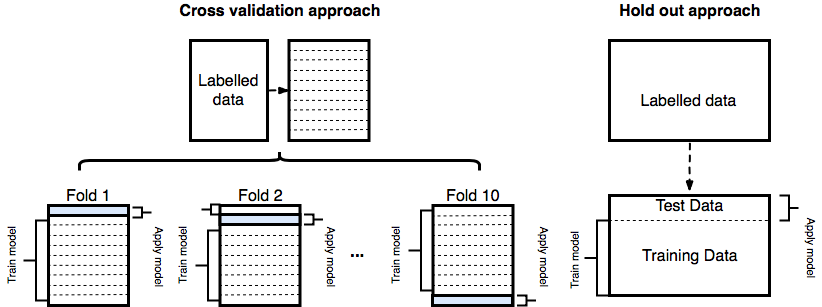
\includegraphics[width=1\linewidth]{images/PatientLevelPrediction/theory/validationTypes} \caption{Types of internal valdiation.}\label{fig:figuretheoryval}
\end{figure}

External validation is when a model trained on one dataset is validated
on a new dataset or set of patients. This is important as it helps model
developers understand which types of patients the model will transport
to.

\begin{figure}
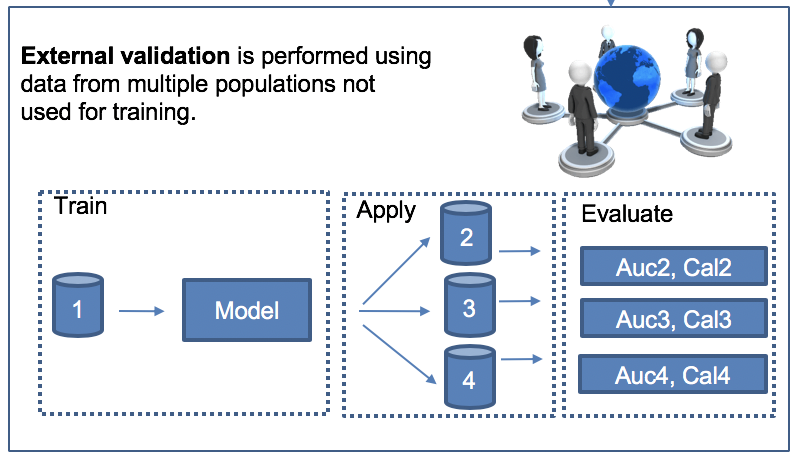
\includegraphics[width=1\linewidth]{images/PatientLevelPrediction/theory/externalValidation} \caption{Visulisation of external validation.}\label{fig:figuretheoryextval}
\end{figure}

Temporal validation is a type of validation where a model is validated
on data that were collected after the data used to develop the model.
This can help identify situations where they may be temporal shifts in
the data that impact the transportability of the model across time.
Another type of validation, spatial validation, is location based where
a model is developed on patients for some locations (perhaps certain
hospitals or doctor surgeries) and validated on patients at a different
location.

\subsubsection{Performance Metrics}\label{performance-metrics}

A prediction model assigned a value between 0 and 1 for each patient
corresponding to the risk of the patient having the outcome during the
time at risk. A value of 0 means 0\% risk, a value of 0.5 means 50\%
risk and a value of 1 means 100\% risk. Common metrics such as accuracy,
sensitivity, specificity, positivity predictive value can be calculated
by first specifying a threshold that is used to class patients as having
the outcome or not having the outcome during the time at risk. For
example, given Table \ldots{}, if we set the threshold as 0.5, the
patients 1,3,7 and 10 have a predicted risk greater than or equal to the
threshold of 0.5 so they would be predicted to have the outcome. All
other patients had a predicted risk less than 0.5, so would be predicted
to not have the outcome.

\begin{figure}
\includegraphics[width=1\linewidth]{images/PatientLevelPrediction/theory/exampleTable} \caption{Example performance table.}\label{fig:figuretheorytab}
\end{figure}

If a patient is predicted to have the outcome and has the outcome during
TAR then this is called as a true positive (TP). If a patient is
predicted to have the outcome but does not have the outcome during TAR
then this I called a false positive (FP). If a patient is predicted to
not have the outcome and does not have the outcome during TAR then this
is called a true negative (TN). Finally, if a patient is predicted to
not have the outcome but does have the outcome during TAR then this is
called a false negative (FN).

The following threshold based metrics are:

\begin{itemize}
\tightlist
\item
  accuracy: (TP+TN)/(TP+TN+FP+FN)
\item
  sensitivity: TP/(TP+FN)
\item
  specificity: TN/(TN+FP)
\item
  positive predictive value: TP/(TP+FP)
\end{itemize}

There are two main criteria used to assess a prediction model;
discrimination and calibration.

Discrimination is the ability to assign a higher risk to patients who
will experience the outcome during the time at risk, where the area
under the receiver operating characteristic curve (AUROC) gives an
overall measure of discrimination where a value of 0.5 corresponds to
randomly assigning the risk and a value of 1 means perfect
discrimination. In reality, most prediction models obtain AUCs between
0.6-0.8. The AUC is calculated by plotting 1 -- specificity on the
x-axis and sensitivity on the y-axis at all possible thresholds. This
generated a plot as seen in Figure \ldots{} and the area under the line
is the AUROC. The AUROC is invariant to class imbalance, unlike
accuracy, but for rare outcomes even a model with a high AUROC may not
be practical. When the outcome is rare another measure known as the area
under the precision recall curve (AUPRC) is recommended. A model may
obtain a high AUC when the outcome is rare but have a very low positive
predictive value. This would mean may false positives. Depending on the
severity of the outcome and cost (health risk and/or monetary) of some
intervention, a low false positive rate may result in a non-practical
model. The AUPRC is the area under the line generated by plotting the
sensitivity on the x-axis (also known as the recall) and the positive
predictive value (also known as the precision) on the y-axis.

The AUROC provides a way to determine how different the predicted risk
distributions are between the patients who experience the outcome during
the time at risk and those who do not. If the AUROC is high, then the
distributions will be mostly disjointed, whereas when there is a lot of
overlap, the AUROC will be closer to 0.5:

\begin{figure}
\includegraphics[width=1\linewidth]{images/PatientLevelPrediction/theory/roctheory} \caption{How the ROC plots are linked to discrimination.}\label{fig:figuretheoryroctheory}
\end{figure}

\begin{figure}
\includegraphics[width=1\linewidth]{images/PatientLevelPrediction/theory/discrimination} \caption{Example discrimination plots generated by the patient-level prediction framework.}\label{fig:figuretheoryroc}
\end{figure}

Calibration is the ability of the model to assign a correct risk. For
example, if the model assigned one hundred patients a risk of 10\% then
ten of the patients should experience the outcome during the time at
risk. If the model assigned 100 patients a risk of 80\% then eighty of
the patients should experience the outcome during the time at risk. The
calibration is generally calculated by partitioning the patients into
deciles based on the predicted risk and in each group calculating the
mean predicted risk and the fraction of the patients who experienced the
outcome during the time at risk. We then plot these ten points
(predicted risk on the y-axis and observed risk on the x-axis) and see
whether they fall on the x = y line, indicating the model is well
calibrated. We also fit a linear model using the points to calculate the
intercept (which should be close to 0) and the gradient (which should be
close to 1). If the gradient is greater than 1 then the model is
assigning a higher risk than the true risk and if the gradient is less
than 1 the model is assigning a lower risk than the true risk.

\begin{figure}
\includegraphics[width=1\linewidth]{images/PatientLevelPrediction/theory/calibration} \caption{Example calibration plots generated by the patient-level prediction framework.}\label{fig:figuretheorycal}
\end{figure}

It can also be useful to determine how well calibrated a model is for
different demographics (age and gender groups). This can be calculated
by partitioning the patients into groups of similar age and gender and
comparing the mean predicted risk within the group with the observed
fraction of the patients who experience the outcome during the time at
risk. This can identify demographic groups where the model does not
perform well when applied.

\newpage 

\section{Specfifying a Patient-level Prediction
Study}\label{specfifying-a-patient-level-prediction-study}

In this section we will demonstrate how to define a prediction problem
using an example for hypertension.

The first step is to clearly define the prediction problem.
Interestingly, in many published papers the prediction problem is poorly
defined, e.g.~it is unclear how the index date (start of the target
Cohort) is defined. A poorly defined prediction problem does not allow
for external validation by others let alone implementation in clinical
practice. In the PLP framework we have enforced that we have to define
the prediction problem we like to address, in which population we will
build the model, which model we will build and how we will evaluate its
performance. In this section we will guide you through this process and
we will use a ``Treatment safety'' prediction type as an example.

\subsection{Problem definition}\label{problem-definition-2}

Angioedema is a well known side-effect of ACE inhibitors, and the
incidence of angioedema reported in the labeling for ACE inhibitors is
in the range of 0.1\% to 0.7\% \citep{byrd_2006}. Monitoring patients
for this adverse effect is important, because although angioedema is
rare, it may be life-threatening, leading to respiratory arrest and
death \citep{norman_2013}. Further, if angioedema is not initially
recognized, it may lead to extensive and expensive workups before it is
identified as a cause \citep{norman_2013, thompson_1993}. Other than the
higher risk among African-American patients, there are no known
predisposing factors for the development of ACE inhibitor related
angioedema \citep{byrd_2006}. Most reactions occur within the first week
or month of initial therapy and often within hours of the initial dose
\citep{circardi_2004}. However, some cases may occur years after therapy
has begun \citep{mara_1996}.No diagnostic test is available that
specifically identifies those at risk. If we could identify those at
risk, doctors could act, for example by discontinuing the ACE
inhibitorin favor of another hypertension drug.

We will apply the PLP framework to observational healthcare data to
address the following patient-level prediction question:

\begin{quote}
Amongst patients who have just started on an ACE inhibitor for the first
time, who will experience angioedema in the following year?
\end{quote}

\subsection{Study population
definition}\label{study-population-definition}

The final study population in which we will develop our model is often a
subset of the target population, because we will e.g.~apply criteria
that are dependent on T and O or we want to do sensitivity analyses with
subpopulations of T. For this we have to answer the following questions:

\begin{itemize}
\item
  \emph{What is the minimum amount of observation time we require before
  the start of the target cohort?} This choice could depend on the
  available patient time in your training data, but also on the time you
  expect to be available in the data sources you want to apply the model
  on in the future. The longer the minimum observation time, the more
  baseline history time is available for each person to use for feature
  extraction, but the fewer patients will qualify for analysis.
  Moreover, there could be clinical reasons to choose a short or longer
  lookback period. For our example, we will use a prior history as
  lookback period (washout period).
\item
  \emph{Can patients enter the target cohort multiple times?} In the
  target cohort definition, a person may qualify for the cohort multiple
  times during different spans of time, for example if they had
  different episodes of a disease or separate periods of exposure to a
  medical product. The cohort definition does not necessarily apply a
  restriction to only let the patients enter once, but in the context of
  a particular patient-level prediction problem, a user may want to
  restrict the cohort to the first qualifying episode. In our example, a
  person can only enter the target cohort once since our criteria was
  based on first use of an ACE inhibitor.
\item
  \emph{Do we allow persons to enter the cohort if they experienced the
  outcome before?} Do we allow persons to enter the target cohort if
  they experienced the outcome before qualifying for the target cohort?
  Depending on the particular patient-level prediction problem, there
  may be a desire to predict incident first occurrence of an outcome, in
  which case patients who have previously experienced the outcome are
  not at-risk for having a first occurrence and therefore should be
  excluded from the target cohort. In other circumstances, there may be
  a desire to predict prevalent episodes, whereby patients with prior
  outcomes can be included in the analysis and the prior outcome itself
  can be a predictor of future outcomes. For our prediction example, we
  will choose not to include those with prior angioedema.
\item
  \emph{How do we define the period in which we will predict our outcome
  relative to the target cohort start?} We actually have to make two
  decisions to answer that question. First, does the time-at-risk window
  start at the date of the start of the target cohort or later?
  Arguments to make it start later could be that you want to avoid
  outcomes that were entered late in the record that actually occurred
  before the start of the target cohort or you want to leave a gap where
  interventions to prevent the outcome could theoretically be
  implemented. Second, you need to define the time-at-risk by setting
  the risk window end, as some specification of days offset relative to
  the target cohort start or end dates. For our problem we will predict
  in a time-at-risk window starting 1 day after the start of the target
  cohort up to 365 days later.
\item
  \emph{Do we require a minimum amount of time-at-risk?} We have to
  decide if we want to include patients that did not experience the
  outcome but did leave the database earlier than the end of our
  time-at-risk period. These patients may experience the outcome when we
  do not observe them. For our prediction problem we decide to answer
  this question with Yes, require a mimimum time-at-risk for that
  reason. Furthermore, we have to decide if this constraint also applies
  to persons who experienced the outcome or we will include all persons
  with the outcome irrespective of their total time at risk. For
  example, if the outcome is death, then persons with the outcome are
  likely censored before the full time-at-risk period is complete.
\end{itemize}

\subsection{Model development
settings}\label{model-development-settings}

To develop the model we have to decide which algorithm(s) we like to
train. We see the selection of the best algorithm for a certain
prediction problem as an empirical question, i.e.~you need to let the
data speak for itself and try different approaches to find the best one.
There is no algorithm that will work best for all problems (no free
lunch). In our framework we therefore aim to implement many algorithms.
Furthermore, we made the system modular so you can add your own custom
algorithms. This out-of-scope for this chapter but mode details can be
found in the \emph{AddingCustomAlgorithms} vignette in the
\href{https://ohdsi.github.io/PatientLevelPrediction/}{PatientLevelPrediction}
package.

Our framework currently contains the following algorithms to choose
from:

Furthermore, we have to decide on the \textbf{covariates} that we will
use to train our model. In our example, we like to add gender, age, all
conditions, drugs and drug groups, and visit counts. We also have to
specify in which time windows we will look and we decide to look in year
before and any time prior.

\subsection{Model evaluation}\label{model-evaluation}

Finally, we have to define how we will train and test our model on our
data, i.e.~how we perform \textbf{internal validation}. For this we have
to decide how we divide our dataset in a training and testing dataset
and how we randomly assign patients to these two sets. Dependent on the
size of the training set we can decide how much data we like to use for
training, typically this is a 75\% - 25\% split. If you have very large
datasets you can use more data for training. To randomly assign patients
to the training and testing set, there are two commonly used approaches:

\begin{enumerate}
\def\labelenumi{\arabic{enumi}.}
\tightlist
\item
  split by person. In this case a random seed is used to assign the
  patient to either sets.
\item
  split by time. In this case a time point is used to split the persons,
  e.g.~75\% of the data is before and 25\% is after this date. The
  advantage of this is that you take into consideration that the health
  care system has changed over time.
\end{enumerate}

For our prediction model we decide to start with a Regularized Logistic
Regression and will use the default parameters. We will do a 75\%-25\%
split by person.

\subsection{Study summary}\label{study-summary-1}

We now completely defined our study as shown in Table
\ref{tab:plpSummary}.

\begin{longtable}[]{@{}ll@{}}
\caption{\label{tab:plpSummary} Main design choices for our
study.}\tabularnewline
\toprule
\begin{minipage}[b]{0.23\columnwidth}\raggedright\strut
Choice\strut
\end{minipage} & \begin{minipage}[b]{0.71\columnwidth}\raggedright\strut
Value\strut
\end{minipage}\tabularnewline
\midrule
\endfirsthead
\toprule
\begin{minipage}[b]{0.23\columnwidth}\raggedright\strut
Choice\strut
\end{minipage} & \begin{minipage}[b]{0.71\columnwidth}\raggedright\strut
Value\strut
\end{minipage}\tabularnewline
\midrule
\endhead
\begin{minipage}[t]{0.23\columnwidth}\raggedright\strut
Target cohort\strut
\end{minipage} & \begin{minipage}[t]{0.71\columnwidth}\raggedright\strut
Patients who have just started on an ACE inhibitor for the first
time.\strut
\end{minipage}\tabularnewline
\begin{minipage}[t]{0.23\columnwidth}\raggedright\strut
Outcome cohort\strut
\end{minipage} & \begin{minipage}[t]{0.71\columnwidth}\raggedright\strut
Angioedema.\strut
\end{minipage}\tabularnewline
\begin{minipage}[t]{0.23\columnwidth}\raggedright\strut
Time-at-risk\strut
\end{minipage} & \begin{minipage}[t]{0.71\columnwidth}\raggedright\strut
1 day till 365 days from cohort start. We will require at least 364 days
at risk.\strut
\end{minipage}\tabularnewline
\begin{minipage}[t]{0.23\columnwidth}\raggedright\strut
Model\strut
\end{minipage} & \begin{minipage}[t]{0.71\columnwidth}\raggedright\strut
Gradient Boosting Machine with hyper-parameters ntree: 5000, max depth:
4 or 7 or 10 and learning rate: 0.001 or 0.01 or 0.1 or 0.9. Covariates
will include gender, age, conditions, drugs, drug groups, and visit
count. Data split: 75\% train - 25\% test, randomly assigned by
person.\strut
\end{minipage}\tabularnewline
\bottomrule
\end{longtable}

We define the target cohort as the first exposure to any ACE inhibitor.
Patients are excluded if they have less than 365 days of prior
observation time or have prior angioedema.

\newpage

\section{Implementing a Patient-level Prediction
Study}\label{implementing-a-patient-level-prediction-study}

There are two ways to use the OHDSI tools for patient-level prediction.
The first approach is to use the atlas interface to design a study and
then atlas creates an R package that goes end to end from data
extraction to model develoment and evaluation. This requires only basic
R knowledge. The second approach is to manually write R code using our
PatientLevelPrediction R library. This requires intermediate R knowledge
at a minimum, but enables greater flexibility in the prediction analysis
study design. In this section, we will provide step-by-step guides for
both approaches.

\subsection{Implementing the study in
Atlas}\label{implementing-the-study-in-atlas}

\subsubsection{Introduction}\label{introduction-1}

The atlas interface to patient-level prediction enables a users to
design a prediction study analysis containing multiple prediction
questions and analyses settings. The atlas interface creates a
prediction study R package populated with all the code ready to develop
and evaluate the specified models. All a user needs to develop the
models is R studio with:

\begin{itemize}
\tightlist
\item
  OHDSI's PatientLevelPrediction R package installed
\item
  devtools R package installed
\item
  connection details for the OMOP CDM databases
\end{itemize}

The atlas created prediction study R package has additional
functionality to:

\begin{itemize}
\tightlist
\item
  Create a study protocol template
\item
  Create a shiny app for interactively exploring the results
\item
  Create a validation study R package that can be shared to externally
  validate the developed models
\end{itemize}

In this section we will detail the design choices for the prediction
problem specification, the analysis settings and the executing settings.
We will then guide the user through the process of reviewing analysis,
downloading and running the prediction study package and interpreting
the results via the shiny app.

\subsubsection{The Atlas layout}\label{the-atlas-layout}

The interface for designing a prediction study can be opened by clicking
on the `Prediction' button in the left hand side atlas menu.

\begin{figure}
\includegraphics[width=1\linewidth]{images/PatientLevelPrediction/atlasImplementation/Atlas_home_prediction} \caption{The Atlas home page.}\label{fig:figure2a}
\end{figure}

Once in the `Prediction' view you should see:

\begin{figure}
\includegraphics[width=1\linewidth]{images/PatientLevelPrediction/atlasImplementation/prediction_page} \caption{The Atlas prediction page.}\label{fig:figure2b}
\end{figure}

You can create a new study by clicking on the blue `New Patient Level
Prediction'`button or by clicking on a row in the table with the name of
the study you want to open. Once inside the prediction study (either by
clicking the blue 'New Patient Level Prediction'`button or an existing
row in the table) you should see a specification option with the top
stating 'Patient Level Prediction' with a number such as `\#52'. This
tells us the cohort definition id is 52.

\begin{figure}
\includegraphics[width=1\linewidth]{images/PatientLevelPrediction/atlasImplementation/prediction_cohort_id} \caption{Where to find the cohort definition id of the prediction study in atlas.}\label{fig:figure2c}
\end{figure}

To the right of the `Patient Level Prediction \#52' there are buttons to
save (green button), exit (blue button with x), copy (blue button with
double paper) and delete (red button with bin) the current study.

\begin{figure}
\includegraphics[width=1\linewidth]{images/PatientLevelPrediction/atlasImplementation/prediction_saveexitcopydelete} \caption{The save/exit/copy/delete options for the prediction study}\label{fig:figure2d}
\end{figure}

Below these is a white text form where you can name the study:

\begin{figure}
\includegraphics[width=1\linewidth]{images/PatientLevelPrediction/atlasImplementation/prediction_naming} \caption{How to name a prediction study}\label{fig:figure2e}
\end{figure}

The `Specification' tab contains all the settings a user needs to define
for the prediction study. The first part is the `Prediction Problem
Settings', this is where the user defines the Target cohorts and Outcome
cohorts for the prediction analyses. These cohorts need to be created in
atlas using the `Cohort Definition' view and can then be imported into
the Prediction study. Instantiating cohorts is described in Chapter
\ref{Cohorts}.

\begin{figure}
\includegraphics[width=1\linewidth]{images/PatientLevelPrediction/atlasImplementation/Spec_prediction_problem_spec} \caption{The Prediction Problem Settings area}\label{fig:figure2f}
\end{figure}

The next part of the `Specification' is the `Analysis Settings'. This is
where the user specifies the models to train (classifiers or survival
models), the candidate covariates (these are standard OHDSI covariates),
the time-at-risk and additional inclusion criteria:

\begin{figure}
\includegraphics[width=1\linewidth]{images/PatientLevelPrediction/atlasImplementation/Spec_analysis_settings} \caption{The Analysis Setting area}\label{fig:figure2g}
\end{figure}

Then the `Execution Settings' define how many patients to extract for
the model development, whether to remove rare covariates and whether to
normalise the covariates:

\begin{figure}
\includegraphics[width=1\linewidth]{images/PatientLevelPrediction/atlasImplementation/Spec_executing_settings} \caption{The Execution Settings area}\label{fig:figure2h}
\end{figure}

Finally, the last part in the `Specification' is the `Training Settings'
which specifies' how to split the labelled data into data used to
develop the model (including how many folds you want to use when
applying cross validation) and validate the model:

\begin{figure}
\includegraphics[width=1\linewidth]{images/PatientLevelPrediction/atlasImplementation/Spec_training_settings} \caption{The Training Settings area}\label{fig:figure2i}
\end{figure}

Each of the `Specification' settings are described in more detail in the
following sections. We also describe the `Utilities' tab where a user
can review, import/export and download their study as an executional R
library.

\subsubsection{Atlas Specification Tab}\label{atlas-specification-tab}

The specification section is where a user can specify her prediction
question, covariates, additional study population inclusion criteria,
model type and hyper-parameters and execution settings.

\paragraph{Prediction Problem
Settings}\label{prediction-problem-settings}

The prediction problem settings enables you to select the target
population cohorts and outcome cohorts for the analysis. A prediction
model will be developed for all combinations of the target population
cohorts and the outcome cohorts.

For example, if you specify two target populations:

\begin{itemize}
\tightlist
\item
  `T1: new users of ACE inhibitors'
\item
  `T2: new users of ACE inhibitors with no prior anti-hypertensive'
\end{itemize}

and three outcomes:

\begin{itemize}
\tightlist
\item
  `O1: angioedema'
\item
  `O2: stroke'
\item
  `O3: myocardial infarction'
\end{itemize}

then six prediction problems will be investigated in the study:

\begin{itemize}
\tightlist
\item
  `In T1: new users of ACE inhibitors predict O1: angioedema during TAR'
\item
  `In T1: new users of ACE inhibitors predict O1: stroke during TAR'
\item
  `In T1: new users of ACE inhibitors predict O1: myocardial infarction
  during TAR'
\item
  `In T2: new users of ACE inhibitors with no prior anti-hypertensive
  predict O1: angioedema during TAR'
\item
  `In T2: new users of ACE inhibitors with no prior anti-hypertensive
  predict O1: stroke during TAR'
\item
  `In T2: new users of ACE inhibitors with no prior anti-hypertensive
  predict O1: myocardial infarction during TAR'
\end{itemize}

To select a target population cohort you need to have previously defined
it atlas. Instantiating cohorts is described in Chapter \ref{Cohorts}.
The Appendix provides the full definitions of the target (Appendix
\ref{AceInhibitors}) and outcome (Appendix \ref{Angioedema}) cohorts
used in this example. To add a target population to the cohort you then
need to click on the blue `+ Add Target Cohort' button:

\begin{figure}
\includegraphics[width=1\linewidth]{images/PatientLevelPrediction/atlasImplementation/prediction_problemSettings_adding_cohort} \caption{The Training Settings area}\label{fig:figure2j}
\end{figure}

This will open up a table of cohorts that have been created in atlas:

\begin{figure}
\includegraphics[width=1\linewidth]{images/PatientLevelPrediction/atlasImplementation/target_pop_cohort_table} \caption{The Training Settings area}\label{fig:figure2k}
\end{figure}

You can simple click on any row in the table to add that cohort. If you
have many cohorts, using the filter option on the top right may help
(just make sure to remember the cohort name). We filtered the book of
ohdsi cohorts by adding `book' to the filter as the cohort names all
included the work `book':

\begin{figure}
\includegraphics[width=1\linewidth]{images/PatientLevelPrediction/atlasImplementation/target_pop_cohort_filter} \caption{The Training Settings area}\label{fig:figure2l}
\end{figure}

By clicking on the row `{[}BookOfOHDSI{]} New users of ACE inhibitors as
first-line monotherapy for hypertension' this is now added as a target
population cohort in the study:

\begin{figure}
\includegraphics[width=1\linewidth]{images/PatientLevelPrediction/atlasImplementation/target_pop_added} \caption{The Training Settings area}\label{fig:figure2m}
\end{figure}

This process can be repeated to add more target population cohorts.
Adding outcome cohorts is a similar process, but requires click on the
blue `+ Add Outcome Cohort' button:

\begin{figure}
\includegraphics[width=1\linewidth]{images/PatientLevelPrediction/atlasImplementation/prediction_problemSettings_adding_outcome_cohort} \caption{The Training Settings area}\label{fig:figure2n}
\end{figure}

You need to specify, at minimum, one target population cohort and one
outcome cohort:

\begin{figure}
\includegraphics[width=1\linewidth]{images/PatientLevelPrediction/atlasImplementation/completed_problem_specification} \caption{The Training Settings area}\label{fig:figure2o}
\end{figure}

Once you have added all the target population cohorts and outcome
cohorts you are now ready to procede to the analysis settings.

\paragraph{Analysis Settings}\label{analysis-settings}

The analysis settings enables you to pick the supervised learning
models, the covariates and population settings.

\subparagraph{Model Settings}\label{model-settings}

You can pick one or more supervised learning models to investigate using
for model development. To add a supervised learning model click on the
blue `+ Add Model Settings' button. A dropdown containing all the models
currently supported in the Atlas interface will appear (note: more
models may be available outside of Atlas);

\begin{figure}
\includegraphics[width=1\linewidth]{images/PatientLevelPrediction/atlasImplementation/analysis_add_model} \caption{Adding a supervised learning model}\label{fig:figureAS1}
\end{figure}

You can select the supervised learning model you want to include in the
study by clicking on the name in the dropdown menu. This will then take
you to a view for that specific model and the hyper-parameters you can
include into a grid search. For example, if I click on `Lasso Logistic
Regression' the following view will appear:

\begin{figure}
\includegraphics[width=1\linewidth]{images/PatientLevelPrediction/atlasImplementation/analysis_lasso_lr_view} \caption{The lasso logistic regression view}\label{fig:figureAS2}
\end{figure}

As the Lasso Logistic Regression model only has one hyper-parameter, we
do an automatic search for the optimal value rather than a grid search
so a user just needs to specify the starting value, see Figure
\ref{fig:figureAS2}. Once you are happy with the hyper-parameter
settings you can return to the main settings view by clicking on the
grey `\textless{}' button:

\begin{figure}
\includegraphics[width=1\linewidth]{images/PatientLevelPrediction/atlasImplementation/analysis_back_from_model_view} \caption{Returning from the lasso logistic regression view}\label{fig:figureAS3}
\end{figure}

You will now see your chosen supervised learning model added:

\begin{figure}
\includegraphics[width=1\linewidth]{images/PatientLevelPrediction/atlasImplementation/analysis_with_model} \caption{The analysis settings with a model added}\label{fig:figureAS4}
\end{figure}

To edit the model you added, click on the corresponding row and it will
take you back to the model view where you can edit the hyper-parameter
settings.

To add a gradient boosting machine model we can follow the same process
and click on `Gradient Boosting Machine' in the drop down menu. This
will take us into the gradient boosting machine view:

\begin{figure}
\includegraphics[width=1\linewidth]{images/PatientLevelPrediction/atlasImplementation/analysis_gbm_view} \caption{The gradient boosting machine view}\label{fig:figureAS5}
\end{figure}

The gradient boosting machine model has four hyper-parameters you can
define a grid search for (boosting learn rate, maximum number of
interactions, minimum number of trees and number of trees to build).
Initially the default values are shown, but a user can add a new value
by typing it into the text field at the bottom of the hyper-parameter
box and clicking on the blue `Add' button.\\

\begin{figure}
\includegraphics[width=1\linewidth]{images/PatientLevelPrediction/atlasImplementation/analysis_adding_hyper} \caption{Adding a hyper-parameter value into the grid search}\label{fig:figureAS6}
\end{figure}

It is also possible to remove a hyper-parameter value from the grid
search by clicking on `Remove' for the corresponding row:

\begin{figure}
\includegraphics[width=1\linewidth]{images/PatientLevelPrediction/atlasImplementation/analysis_removing_hyper} \caption{Removing a hyper-parameter value into the grid search}\label{fig:figureAS7}
\end{figure}

Once happy with the hyper-parameters, click on the grey `\textless{}'
button on the top left to add the model into the prediction study. You
will now see you model and hyper-parameter settings in the `Model
Setttings' table. Repeat the process to include all the supervised
learning models you want to investigate.

\subparagraph{Covariate Settings}\label{covariate-settings}

We have defined a set of \emph{standard} covariates that can be
extracted from the observational data in the OMOP CDM format. In the
covariate settings view, it is possible to select which of the standard
covariates to include. It is possible to add many different types of
covariate settings.

To add a covariate setting into the study, click on the blue `+ Add
Covariate Settings' button:

\begin{figure}
\includegraphics[width=1\linewidth]{images/PatientLevelPrediction/atlasImplementation/analysis_adding_covariate} \caption{Adding a covariate setting specification}\label{fig:figureAS8}
\end{figure}

This will take you into the covariate setting view:

\begin{figure}
\includegraphics[width=1\linewidth]{images/PatientLevelPrediction/atlasImplementation/analysis_covariate_view} \caption{The covariate settings view}\label{fig:figureAS9}
\end{figure}

The \emph{standard} OHDSI covariates includes indicator covariates
corresponding to any concept id that is recorded in the database. The
indicator covariates are binary and indicate whether a patient had a
concept id recorded during some time interval relative to the target
cohort start date. The user can specify up to three time intervals,
longterm, mediumterm and shortterm in addition to using anytime prior.
There is also the option of whether to include the target cohort start
date:

{[}add picture{]}

Although the \emph{standard} OHDSI covariates iclude 4 time intervals
(all time prior, longterm, mediumterm and short term) and all concept
ids, generally only a subset of these covariates will be chosen. The
concept ids can be restricted by OHDSI vocabulary domain (condition,
drug, procedure, measurement and observation). Generally, a user will
select one or two time intervals and some of the domains. For example,
if a user selects long term (using default set to 365 days prior)
conditions and drugs and anytime prior measurements with end days set to
0, then there could be covariates for any condition or drug concept id
record 365 days prior to and up to the cohort start day for any patient
in the target cohort and covariates for any measurement concept id
recorded on the cohort start day or anytime prior.

Age group and gender are also binary covariates, with age group
covariates for every 5 years (0-4, 5-9, 10-14, \ldots{}, 95+).

Non binary covariates include age, domain counts, such as the number of
condition concept ids were recorded for each time interval per patient
or the number of inpatient visits a patient had during the time
interval. Measurement covaraites can be binary (indicating a measurement
was taken or whether it was abnormal) or non-binary (the value of the
measurement). Existing risk scores can also be chosen.

\textbf{Include/Exclude options}

The first part is of the covariate settings is the exclude/include
option.\\

\begin{figure}
\includegraphics[width=1\linewidth]{images/PatientLevelPrediction/atlasImplementation/analysis_covariate_include_exclude} \caption{The option to specify concepts/covariates to only include or to exclude}\label{fig:figureAS11}
\end{figure}

Above we mentioned that covariates are generally constructed for any
concept id in the chosen time intervals and domains. However, you may be
in a situation where you only want to include certain concept ids or you
may want to exlcude concept ids (e.g., if the concept id is linked to
the target cohort definition).

To only include certain concepts, create a concept set in atlas and then
under the ``What concepts do you want to include in baseline covariates
in the patient-level prediction model? (Leave blank if you want to
include everything)'' select the concept set by clicking on the blue
button with a folder icon:

\begin{figure}
\includegraphics[width=1\linewidth]{images/PatientLevelPrediction/atlasImplementation/analysis_covariate_include_folder} \caption{The option to specify concepts/covariates to only include or to exclude}\label{fig:figureAS12}
\end{figure}

this will then open up a table with all the concept sets, select the one
you want. You can include the concept ids in the concept set and all
descendants by select `yes' to the ``Should descendant concepts be added
to the list of included concepts?'' option. This option will mean after
you select the covariates you want, only covariates corresponding to
these included concept ids will be included.

The same process can be repeated for the ``What concepts do you want to
exclude in baseline covariates in the patient-level prediction model?
(Leave blank if you want to include everything)'' but this will mean
after you select the covariates you want, any covariates corresponding
to these concept ids will be removed.

To remove any include/exclude setting, click on the red button with an
X.

The final option ``A comma delimited list of covariate IDs that should
be restricted to:'' enables you to add a set of covariate ids (rather
than concept ids) comma seperated that will only be included in the
model. For example if you wanted covariate ids 340504504 and 8373747504
then you would type ``340504504,8373747504'' into the text box. You must
ensure the domain/time interval corresponding to these covariates are
selected below.

\textbf{Non time bound options}

The next section enables the selection of non-time bound variables:

\begin{itemize}
\tightlist
\item
  Gender: a binary variable indicating male or female gender
\item
  Age: a continuous variable corresponding to age in years
\item
  Age group: binary variables for every 5 years of age (0-4, 5-9, 10-14,
  \ldots{}, 95+)
\item
  Race: a binary variable for each race, 1 means the patient has that
  race recorded, 0 otherwise
\item
  Ethnicity: a binary variable for each ethnicity, 1 means the patient
  has that ethnicity recorded, 0 otherwise
\item
  Index year: {[}Not recommended for prediction{]} a binary variable for
  each cohort start date year, 1 means that was the patients cohort
  start date year, 0 otherwise
\item
  Index month - a binary variable for each cohort start date month, 1
  means that was the patients cohort start date month, 0 otherwise
\item
  Prior observation time: {[}Not recommended for prediction{]} a
  continuous variable corresponding to how long in days the patient was
  in the database prior to the cohort start date
\item
  Post observation time: {[}Not recommended for prediction{]} a
  continuous variable corresponding to how long in days the patient was
  in the database post cohort start date
\item
  Time in cohort: a continuous variable corresponding to how long in
  days the patient was in the cohort (cohort end date minus cohort start
  date)
\item
  Index year and month: {[}Not recommended for prediction{]} a binary
  variable for each cohort start date year and month combination, 1
  means that was the patients cohort start date year and month, 0
  otherwise
\end{itemize}

To include any of these variables, click the corresponding unticked box
to add a tick (clicking a ticked box will remove the variable):

\begin{figure}
\includegraphics[width=1\linewidth]{images/PatientLevelPrediction/atlasImplementation/analysis_covariates_nontime} \caption{The option to include non-time bound variables}\label{fig:figureAS13}
\end{figure}

\textbf{Time interval options}

The standard covariates enable three flexible time intervals for the
covariates:

\begin{itemize}
\tightlist
\item
  end days: when to end the time intervals relative to the cohort start
  date {[}default is 0{]}
\item
  long term {[}default -365 days to end days prior to cohort start
  date{]}
\item
  medium term {[}default -180 days to end days prior to cohort start
  date{]}
\item
  short term {[}default -30 days to end days prior to cohort start
  date{]}
\end{itemize}

These settings can be input into the text boxes to update them

\begin{figure}
\includegraphics[width=1\linewidth]{images/PatientLevelPrediction/atlasImplementation/analysis_covariates_timeset} \caption{The options to set the time intervals}\label{fig:figureAS14}
\end{figure}

\textbf{Domain covariates}

The next option is the covariates extracted from the era tables:

\begin{itemize}
\tightlist
\item
  Condition: Construct covariates for each condition concept id and time
  interval selected and if a patient has the concept id with an era
  (i.e., the condition starts or ends during the time interval or starts
  before and ends after the time interval) during the specified time
  interval prior to the cohort start date in the condition era table,
  the covariate value is 1, otherwise 0.
\item
  Condition group: Construct covariates for each condition concept id
  and time interval selected and if a patient has the concept id
  \textbf{or any descendant concept id} with an era during the specified
  time interval prior to the cohort start date in the condition era
  table, the covariate value is 1, otherwise 0.
\item
  Drug: Construct covariates for each drug concept id and time interval
  selected and if a patient has the concept id with an era during the
  specified time interval prior to the cohort start date in ths drug era
  table, the covariate value is 1, otherwise 0.
\item
  Drug group: Construct covariates for each drug concept id and time
  interval selected and if a patient has the concept id \textbf{or any
  descendant concept id} with an era during the specified time interval
  prior to the cohort start date in ths drug era table, the covariate
  value is 1, otherwise 0.
\end{itemize}

Click on a box with no tick to add a tick and select that covariate into
the covariate settings. Clicking on a box with a tick with untick it and
remove that covariate from the covaraite settings.

\begin{figure}
\includegraphics[width=1\linewidth]{images/PatientLevelPrediction/atlasImplementation/analysis_covariates_era} \caption{The options to pick the covariates extracted using the era table and vocabulary heirarchy}\label{fig:figureAS15}
\end{figure}

{[}need to check this{]} Overlapping time inverval setting means you
want the drug or condition to start prior to the cohort start date and
end after the cohort start date (so it overlaps with the cohort start
date). The \textbf{era start} option restricts to finding condition or
drug eras that start during the time interval selected.

The domain tables covariates enable you to pick whether to include
covariates corresponding to concept ids in each domain for the various
time intervals:

\begin{itemize}
\tightlist
\item
  Condition: Construct covariates for each condition concept id and time
  interval selected and if a patient has the concept id recorded during
  the specified time interval prior to the cohort start date in the
  condition occurrence table, the covariate value is 1, otherwise 0.
\item
  Condition Primary Inpatient: ?
\item
  Drug: Construct covariates for each drug concept id and time interval
  selected and if a patient has the concept id recorded during the
  specified time interval prior to the cohort start date in the drug
  exposure table, the covariate value is 1, otherwise 0.
\item
  Procedure: Construct covariates for each procedure concept id and time
  interval selected and if a patient has the concept id recorded during
  the specified time interval prior to the cohort start date in the
  procedure occurrence table, the covariate value is 1, otherwise 0.
\item
  Measurement: Construct covariates for each measurement concept id and
  time interval selected and if a patient has the concept id recorded
  during the specified time interval prior to the cohort start date in
  the measurement table, the covariate value is 1, otherwise 0.
\item
  Measurement Value: Construct covariates for each measurement concept
  id with a value and time interval selected and if a patient has the
  concept id recorded during the specified time interval prior to the
  cohort start date in the measurement table, the covariate value is the
  measurement value, otherwise 0.
\item
  Measurement range group: ?
\item
  Observation: Construct covariates for each observation concept id and
  time interval selected and if a patient has the concept id recorded
  during the specified time interval prior to the cohort start date in
  the observation table, the covariate value is 1, otherwise 0.
\item
  Device: Construct covariates for each device concept id and time
  interval selected and if a patient has the concept id recorded during
  the specified time interval prior to the cohort start date in the
  device table, the covariate value is 1, otherwise 0.
\item
  Visit Count: Construct covariates for each visit and time interval
  selected and count the number of visits recorded during the time
  interval as the covariate value
\item
  Visit Concept Count: Construct covariates for each visit, domain and
  time interval selected and count the number of records per domain
  recorded during the visit type and time interval as the covariate
  value
\end{itemize}

The distinct count option counds the number of records per domain and
time interval {[}expand{]}.

\begin{figure}
\includegraphics[width=1\linewidth]{images/PatientLevelPrediction/atlasImplementation/analysis_covariates_main} \caption{The options to pick the covariates from the domain tables}\label{fig:figureAS16}
\end{figure}

\textbf{Risk score covariates}

The final option is whether to include commonly used risk scores as
covariate:

\begin{figure}
\includegraphics[width=1\linewidth]{images/PatientLevelPrediction/atlasImplementation/analysis_covariates_riskscores} \caption{The options to pick existing risk scores as covariates}\label{fig:figureAS17}
\end{figure}

Once happy with the covariate settings, click the `\textless{}' button
on the top left corner to return to the main prediction settings. Your
covariate options you picked will now show in the covaraite settings
table. You can edit an exisitng setting by clicking on the corresponding
row or add more covariate settings by clicking on the blue `+ Add
Covariate Settings' button again.

\subparagraph{Population Settings}\label{population-settings}

The population settings is where addition inclusion criteria can be
applied to the target population (this may be useful for sensitivity
investigations) and is also where the time-at-risk is defined.

To add a population setting into the study, click on the blue `+ Add
Population Settings' button:

\begin{figure}
\includegraphics[width=1\linewidth]{images/PatientLevelPrediction/atlasImplementation/analysis_adding_population} \caption{Adding a population setting specification}\label{fig:figureAS18}
\end{figure}

This will open up the population setting view containing various setting
to define:

\begin{figure}
\includegraphics[width=1\linewidth]{images/PatientLevelPrediction/atlasImplementation/analysis_population_settings} \caption{The population setting options}\label{fig:figureAS19}
\end{figure}

The first set of options, A and B, enable the user to specify the
time-at-risk period. This is a time interval relative to the target
cohort dates where we look to see whether the outcome of interest
occurs. If a patient has the outcome during the time at risk period then
we will class them as `outcome', otherwise they are classed as
`non-outcome'.

The first option labelled with a red A is: ``Define the time-at-risk
window start, relative to target cohort entry:'' - this settings lets
you define the start of the time-at-risk. It is relative to the target
cohort dates (cohort start date or cohort end date). You can pick an
offset corresponding to the number of days and whether it is relative to
the target cohort start date or the target cohort end date.

The second option labelled with a red B is: ``Define the time-at-risk
window end:'' - this settings lets you define the end of the
time-at-risk. It is relative to the target cohort dates (cohort start
date or cohort end date). You can pick an offset corresponding to the
number of days and whether it is relative to the target cohort start
date or the target cohort end date.

See Figure \ref{fig:figureAS20} for an illustration of how these
settings define the time-at-risk period:

\begin{figure}
\includegraphics[width=1\linewidth]{images/PatientLevelPrediction/atlasImplementation/analysis_population_plot} \caption{How the population setting options define the time-at-risk}\label{fig:figureAS20}
\end{figure}

The next option, marked by the red C, is ``Minimum lookback period
applied to target cohort:''. This is where you can specify the minimum
baseline period, specifically the minimum number of days prior to the
cohort start date that a patient has been continuously observed. The
default is 365 days. Expanding the minimum lookback will give a more
complete picture of a patient (as they must have been observed for
longer) but will filter many patienst (who do not have the minimum
number of days prior observation).

The option maked by the red D is ``Should subjects without time at risk
be removed?''. If this is set to yes, then a value for ``Minimum time at
risk:'' is also required. This option lets you deal with people who are
lost to follow-up (e.g., they leave the database during the time-at-risk
period). If you select `yes' then you need to specify the minimum time a
patient needs to be in the time-at-risk period for them to be included
in the labelled data (if they do not have the minimum time they are
excluded from the population). For example, if the time-at-risk period
was 1 day from cohort start until 365 days from cohort start, then the
full time-at-risk interval is 364 days (365-1). If you only want to
include patients who are observed the whole interval, then set the
minimum time at risk to be 364. If you are happy as long as people are
in the time-at-risk for the first 100 days, then select minimum time at
risk to be 100. In this case as the time-at-risk start as 1 day from the
cohort start, a patient will be include if they remain in the database
for at least 101 days from the cohort start date. If you set ``Should
subjects without time at risk be removed?'' to `No', then this will keep
every patient, even those who drop out from the database during the
time-at-risk.

The option E ``Include people with outcomes who are not observed for the
whole at risk period?'' is also linked to D. This option lets you treat
people with the outcome who drop out of the database during time-at-risk
differently to those who do not have the outcome observed before
dropping out. If ``Include people with outcomes who are not observed for
the whole at risk period?'' is set to `No', then people who are not
observed for the whole time-at-risk are include/excluded depending on
your settings for D. However, if ``Include people with outcomes who are
not observed for the whole at risk period?'' is set to `Yes', then this
means people who have the outcome recorded during the time-at-risk
interval are included in the labelled data even if they drop out from
the database before the end of the time-at-risk interval.

The option ``Should only the first exposure per subject be included?''
labelled in F is only useful if you have a target cohort that contains
patients multiple times but with different cohort start dates. In this
situation, picking `yes' for ``Should only the first exposure per
subject be included?'' will result in only keeping the earliest target
cohort date per patient in the analysis (i.e., unique patients);
otherwise a patient can be in the labbelled dataset multiple times but
the covariates and time-at-risk will be at different time points in the
patients observation.

The final option G is ``Remove patients who have observed the outcome
prior to cohort entry?''. Selecting `Yes' to this option will remove
patients who have the outcome prior to the time-at-risk start date, so
the model is in patients who have never experience the outcome prior. If
`No' is selected, then patients could have had the outcome prior.
Generally, having the outcome prior is very predictive of having the
outcome during the time-at-risk.

Once you are happy with the population settings, click on the grey
`\textless{}' button in the top left and this will return you to the
main setting view. You will now see your population settings as a new
row in the population settings table. To edit the settings click on the
corresponding row. This will take you to the population setting view
where you can change any of the settings.

To add more population settings, repeat the process detailed in this
section.

\subparagraph{Execution settings}\label{execution-settings}

Execution settings determine whether to use sampling, how to manage rare
events, and whether to normalize covariates. Sampling can be an
efficient means to determine if a model for a large population (i.e.~10
million patients) is accurate, by creating and testing the model with a
subgroup of patients (e.g.~if AUC is close to 0.5 on your sampling, you
might abandon the model). The user specifies the size of the subgroup to
be sampled. A minimum threshold value for covariate occurrence is
necessary to remove rare events that are not representative of the
overall population. Normalization of the covariates is usually necessary
for successful implementation of a LASSO model.

\begin{figure}
\includegraphics[width=1\linewidth]{images/PatientLevelPrediction/atlasImplementation/analysis_execution_settings} \caption{The execution settings}\label{fig:figureAS21}
\end{figure}

There are three options:

\begin{itemize}
\tightlist
\item
  ``Perform sampling'': here you can choosen whether to perform sampling
  (default = `No'). If you set this to `yes', another option will appear
  ``How many patients to use for a subset?'', here you can add the
  sample size you wish to extract.
\item
  ``Minimum covariate occurrence: If a covariate occurs in a fraction of
  the target population less than this value, it will be removed:'':
  here you can choose then minimum covariate occurrence (default =
  0.001)
\item
  ``Normalize covariate'': here you can choose whether to normalize
  covariates (default = `Yes)
\end{itemize}

\subparagraph{Training settings}\label{training-settings}

Training settings determine how to distribute the data between training
and testing groups. Most of the data will be used to train the model and
the rest will be used to test it. The data can be divided by either unit
person or time. The percentage of data attributed to training or testing
the model is specified by the user (Figure X). Additionally, the number
of folds for cross-validation is specified, which partitions the
training data for hyper-parametric analysis (Figure Y). The user has the
option of specifying the seed used to split the training and testing
data for consistent distribution of the outcomes between the groups.
This option is only needed for person based splitting.

\begin{figure}
\includegraphics[width=1\linewidth]{images/PatientLevelPrediction/atlasImplementation/analysis_training_settings} \caption{The training settings}\label{fig:figureAS22}
\end{figure}

There are four options:

\begin{itemize}
\tightlist
\item
  ``Specify how to split the test/train set:: Select whether to
  differentiate the train/test data by person (stratified by outcome) or
  by time (older data to train the model, later data to evaluate the
  model)
\item
  ``Percentage of the data to be used as the test set (0-100\%)'':
  Select the percentage of data to be used as test data (default = 25\%)
\item
  ``The number of folds used in the cross validation'': Select the
  number of folds for cross-validation (default = 3)
\item
  ``The seed used to split the test/train set when using a person type
  testSplit (optional):'': Select the seed used to split the train/test
  set when using a person type test split
\end{itemize}

{[}add picture of the test/train and cross valdiation{]}

\paragraph{Atlas Utilities Tab}\label{atlas-utilities-tab}

The Utilities tab is where a user can review the prediction study (once
minimum required settings are defined), export/import existing atlas
prediction studies and download the prediction study R package.

\begin{figure}
\includegraphics[width=1\linewidth]{images/PatientLevelPrediction/atlasImplementation/utilities_main} \caption{The utilities tab}\label{fig:figureU1}
\end{figure}

\subparagraph{How to review a study}\label{how-to-review-a-study}

\textbf{Review and Download Tab} If you have not completed all
pre-requisites needed to run the study, you will see the following:

\begin{figure}
\includegraphics[width=1\linewidth]{images/PatientLevelPrediction/atlasImplementation/utilities_review_insuf} \caption{Reviewing when insufficient design}\label{fig:figureU2}
\end{figure}

Assuming your study contains all necessary components, you will see the
following screen, showing the tabs Full Analysis List, Prediction
Problem Settings, and Analysis Settings.

\begin{figure}
\includegraphics[width=1\linewidth]{images/PatientLevelPrediction/atlasImplementation/utilities_review} \caption{The utilities tab reviewing valid study}\label{fig:figureU3}
\end{figure}

Clicking on the Prediction Problem Settings shows the screen below,
showing the respective Target Cohort and Outcome Cohort names:

\begin{figure}
\includegraphics[width=1\linewidth]{images/PatientLevelPrediction/atlasImplementation/utilities_review_prediction} \caption{The utilities tab reviewing the prediction questions in the study}\label{fig:figureU4}
\end{figure}

Finally, clicking on the Analysis Settings tab results in the screen
below, allowing you to review all of the Model Names, Model Settings,
Covariate Settings, Risk Window Start and Risk Window End.

\begin{figure}
\includegraphics[width=1\linewidth]{images/PatientLevelPrediction/atlasImplementation/utilities_review_analysis} \caption{The utilities tab reviewing the analysis settings in the study}\label{fig:figureU5}
\end{figure}

\subparagraph{How to import/export
study}\label{how-to-importexport-study}

To export a study, click on the Export tab under utilities. ATLAS will
produce JSON file that can be directly copied and pasted into a file
that contains all of the data (study name, cohort definitions, models
selected, covariates, settings, etc.) needed to run the study.

\begin{figure}
\includegraphics[width=1\linewidth]{images/PatientLevelPrediction/atlasImplementation/utilities_export} \caption{Exporting a study design}\label{fig:figureU6}
\end{figure}

To import a study, first go back to the main ATLAS menu and click on
Prediction. Click on the New Patient Level Prediction button, give your
study a name, and Save. Next, click on the Utilities tab, then the
Import tab. Paste the contents of a Patient Level Prediction JSON file
into this window, then click on the Import button below the other tab
buttons.

\begin{figure}
\includegraphics[width=1\linewidth]{images/PatientLevelPrediction/atlasImplementation/utilities_import} \caption{Importing a study design}\label{fig:figureU7}
\end{figure}

\subparagraph{How to download package}\label{how-to-download-package}

The Download Study button is available at the bottom of the Utilities
screen. Enter a descriptive name for the R package, noting that any
illegal characters in R will automatically be removed from the file name
by ATLAS.

\begin{figure}
\includegraphics[width=1\linewidth]{images/PatientLevelPrediction/atlasImplementation/utilities_download} \caption{Downloading the study design as an R package}\label{fig:figureU8}
\end{figure}

ATLAS will generate an R package for the study.

\begin{figure}
\includegraphics[width=1\linewidth]{images/PatientLevelPrediction/atlasImplementation/utilities_downloading} \caption{The downloaded study design R package}\label{fig:figureU9}
\end{figure}

\paragraph{Building Atlas created prediction study R
package}\label{building-atlas-created-prediction-study-r-package}

\subparagraph{Setting up R}\label{setting-up-r}

To run the atlas generated prediction R package study requires having R
studio () installed, the devtools R package {[}in R run:
install.packages(`devtools'){]} and the OHDSI PatientLevelPrediction
package installed (see \ldots{}).

\subparagraph{Unzipping atlas compressed
folder}\label{unzipping-atlas-compressed-folder}

Atlas generates a zipped directory containing the R package. This zipped
directory needs to be extracted. Once extracted the directory will look
like:

\begin{figure}
\includegraphics[width=1\linewidth]{images/PatientLevelPrediction/atlasImplementation/download_folder} \caption{The directory of study design R package}\label{fig:figureU10}
\end{figure}

\subparagraph{Opening package project in
R}\label{opening-package-project-in-r}

The easiest way to open the atlas created package in R is to double
click on the project file:

\begin{figure}
\includegraphics[width=1\linewidth]{images/PatientLevelPrediction/atlasImplementation/download_folder_project} \caption{Opening the study design R package}\label{fig:figureU11}
\end{figure}

This will then open a new R studio session:

\begin{figure}
\includegraphics[width=1\linewidth]{images/PatientLevelPrediction/atlasImplementation/rstudio_start} \caption{Rstudio open with the study design project}\label{fig:figureU12}
\end{figure}

\subparagraph{Building project}\label{building-project}

Once R studio has opened the project, you can then build the package by
clicking on the `build' option in the top right hand side:

\begin{figure}
\includegraphics[width=1\linewidth]{images/PatientLevelPrediction/atlasImplementation/building} \caption{Building the R project into a local R library}\label{fig:figureU13}
\end{figure}

If you find a message like (but with the text in red matching the name
you called your study):

\begin{figure}
\includegraphics[width=1\linewidth]{images/PatientLevelPrediction/atlasImplementation/buildComplete} \caption{Building the R project completed}\label{fig:figureU14}
\end{figure}

Your package has now been created and will be available to run. If you
have a message with an error then there was an issue with building the
package and the package did not get built. Common issues causing the
build to fail are missing dependencies, to find out the R packages
required for your built, open the `DESCRIPTION' file in the main
directory:

\begin{figure}
\includegraphics[width=1\linewidth]{images/PatientLevelPrediction/atlasImplementation/download_folder_desc} \caption{Finding the DECSRIPTION file}\label{fig:figureU15}
\end{figure}

This will open up in R studio and show what R packages are required (the
packages in the Imports section)

\begin{figure}
\includegraphics[width=1\linewidth]{images/PatientLevelPrediction/atlasImplementation/description} \caption{The DECSRIPTION file content}\label{fig:figureU16}
\end{figure}

If you do not have any of the packages listed in `Imports:' then you
will need to install them before building the atlas generated package.

\paragraph{Running Study}\label{running-study}

\subparagraph{Readme and
extras/codetorun.R}\label{readme-and-extrascodetorun.r}

The key file in the atlas generated package directory is the one that
contains code for running the study, the CodeToRun.R file found in the
extras directory:

\begin{figure}
\includegraphics[width=1\linewidth]{images/PatientLevelPrediction/atlasImplementation/download_folder_extras} \caption{The CodeToRun.R file is in the extras folder}\label{fig:figureU17}
\end{figure}

We recommend opening the file CodeToRun.R

\begin{figure}
\includegraphics[width=1\linewidth]{images/PatientLevelPrediction/atlasImplementation/code_to_run} \caption{The CodeToRun.R file}\label{fig:figureU18}
\end{figure}

\subparagraph{CodeToRun.R Settings}\label{codetorun.r-settings}

The final step to running the study is to connect to the database
through R and specify where the results should be saved.,

The CodeToRun.R file looks like:

\begin{figure}
\includegraphics[width=1\linewidth]{images/PatientLevelPrediction/atlasImplementation/code_to_run_open} \caption{The CodeToRun.R default setting}\label{fig:figureU19}
\end{figure}

The inputs for the CodeToRun file are:

\begin{itemize}
\tightlist
\item
  outputFolder: This is a string specifying where in your computer to
  save the results. This location needs to have sufficient space as data
  will be extracted from the database into this location and the
  lcoation must have read/write access.
\item
  options(fftempdir = ''): this is a location in your computer that must
  have read/write access and large amounts of space. It will be used to
  store temporary data.
\item
  dbms: The database management system you use
\item
  user: Your username for the database connection (contact database
  administrator if unknown)
\item
  pw: Your password for the database connection (contact database
  administrator if unknown)
\item
  server: a string specifying the database server (contact database
  administrator if unknown)
\item
  port: (optional) the port number (contact database administrator if
  unknown)
\item
  cdmDatabaseSchema: a string specifying the database schema containing
  the OMOP CDM instance
\item
  cohortDatabaseSchema: a string specifying the database schema either
  containing the cohorts or where to create the cohorts.
\item
  oracleTempSchema: if using oracle, this is your temp database schema
\item
  cohortTable: the name of the cohort table (if using atlas cohorts then
  this will be `cohort')
\end{itemize}

Once the settings are filled out, the final step is to pick what parts
of the study to execute:

\begin{figure}
\includegraphics[width=1\linewidth]{images/PatientLevelPrediction/atlasImplementation/execute} \caption{Executing the study}\label{fig:figureU20}
\end{figure}

The following options specify:

\begin{itemize}
\tightlist
\item
  A: createProtocol - set to `True' if you want to create a word
  document protocol template that automatically inserts the study design
  settings. This can be shared if creating a network study.
\item
  B: createCohorts - do you need to create the cohorts for this study?
  If you are using atlas cohorts you can set this to `False' otherwise
  set this to `True' and the cohorts you picked for the study will all
  be generated.
\item
  C: runAnalyses - setting this to `True' will result in models being
  developed and evaluated for each setting you specified in the study
  design. This requires cohorts to have been generated (in atlas or
  using B createCohorts set to `True').
\item
  D: createResultsDoc - if you set A: createProtocol to `True' and
  generated a protocol and also ran the analysis by setting C:
  runAnalyses to `True' then you can add the results into the protocol
  to create a word document with the protocol and results.
\item
  E: packageResults - if you set C: runAnalyses to `True' and have
  results, you can set packageResults to `True' to create a zipped
  folder containing your results with any sensitive data removed. This
  can be easily shared with other OHDSI colabortors.
\item
  F: createValidationPackage - if a model seems to do, we can use this
  option to create a new R package for validating the model. Set to
  `True' to create a validation package containing all the models for
  external validation. In later Atlas versions there is another input
  where you can specify the analysis id of a model rather than
  validating all models.
\item
  G: minCellCount - this is linked to E: packageResults and F:
  createValidationPackage and specifies the minimum cell count for any
  result to be included when sharing the models. For example, if the
  minCellCount is 5, then any count with a value less than 5 will be
  removed.
\end{itemize}

\paragraph{Viewing the Results}\label{viewing-the-results}

After running the R package analysis you can view the results in an
interactive shiny app by running:

\begin{Shaded}
\begin{Highlighting}[]
\NormalTok{PatientLevelPrediction}\OperatorTok{::}\KeywordTok{viewMultiplePlp}\NormalTok{(outputFolder)}
\end{Highlighting}
\end{Shaded}

\newpage

\subsection{Implementing the study in
R}\label{implementing-the-study-in-r}

Now we have completely designed our study we have to implement the study
in R. This will be done using the
\href{https://ohdsi.github.io/PatientLevelPrediction/}{PatientLevelPrediction}
package to build patient-level predictive models. The package enables
data extraction, model building, and model evaluation using data from
databases that are translated into the OMOP CDM.

\subsubsection{Cohort instantiation}\label{cohort-instantiation-1}

We first need to instantiate the target and outcome cohorts.
Instantiating cohorts is described in Chapter \ref{Cohorts}. The
Appendix provides the full definitions of the target (Appendix
\ref{AceInhibitors}) and outcome (Appendix \ref{Angioedema}) cohorts. In
this example we will assume the ACE inhibitors cohort has ID 1, and the
angioedema cohort has ID 2.

\subsubsection{Data extraction}\label{data-extraction-1}

We first need to tell R how to connect to the server.
\href{https://ohdsi.github.io/PatientLevelPrediction/}{\texttt{PatientLevelPrediction}}
uses the
\href{https://ohdsi.github.io/DatabaseConnector/}{\texttt{DatabaseConnector}}
package, which provides a function called
\texttt{createConnectionDetails}. Type \texttt{?createConnectionDetails}
for the specific settings required for the various database management
systems (DBMS). For example, one might connect to a PostgreSQL database
using this code:

\begin{Shaded}
\begin{Highlighting}[]
\KeywordTok{library}\NormalTok{(PatientLevelPrediction)}
\NormalTok{connDetails <-}\StringTok{ }\KeywordTok{createConnectionDetails}\NormalTok{(}\DataTypeTok{dbms =} \StringTok{"postgresql"}\NormalTok{,}
                                       \DataTypeTok{server =} \StringTok{"localhost/ohdsi"}\NormalTok{,}
                                       \DataTypeTok{user =} \StringTok{"joe"}\NormalTok{,}
                                       \DataTypeTok{password =} \StringTok{"supersecret"}\NormalTok{)}

\NormalTok{cdmDbSchema <-}\StringTok{ "my_cdm_data"}
\NormalTok{cohortsDbSchema <-}\StringTok{ "scratch"}
\NormalTok{cohortsDbTable <-}\StringTok{ "my_cohorts"}
\NormalTok{cdmVersion <-}\StringTok{ "5"}
\end{Highlighting}
\end{Shaded}

The last four lines define the \texttt{cdmDbSchema},
\texttt{cohortsDbSchema}, and \texttt{cohortsDbTable} variables, as well
as the CDM version. We will use these later to tell R where the data in
CDM format live, where the cohorts of interest have been created, and
what version CDM is used. Note that for Microsoft SQL Server, database
schemas need to specify both the database and the schema, so for example
\texttt{cdmDbSchema\ \textless{}-\ "my\_cdm\_data.dbo"}.

First it makes sense to verify that the cohort creation has succeeded,
by counting the number of cohort entries:

\begin{Shaded}
\begin{Highlighting}[]
\NormalTok{sql <-}\StringTok{ }\KeywordTok{paste}\NormalTok{(}\StringTok{"SELECT cohort_definition_id, COUNT(*) AS count"}\NormalTok{,}
\StringTok{"FROM @cohortsDbSchema.cohortsDbTable"}\NormalTok{,}
\StringTok{"GROUP BY cohort_definition_id"}\NormalTok{)}
\NormalTok{conn <-}\StringTok{ }\KeywordTok{connect}\NormalTok{(connDetails)}
\KeywordTok{renderTranslateQuerySql}\NormalTok{(}\DataTypeTok{connection =}\NormalTok{ conn, }
                        \DataTypeTok{sql =}\NormalTok{ sql,}
                        \DataTypeTok{cohortsDbSchema =}\NormalTok{ cohortsDbSchema,}
                        \DataTypeTok{cohortsDbTable =}\NormalTok{ cohortsDbTable)}
\end{Highlighting}
\end{Shaded}

\begin{verbatim}
##   cohort_definition_id  count
## 1                    1 527616
## 2                    2   3201
\end{verbatim}

Now we can tell
\href{https://ohdsi.github.io/PatientLevelPrediction/}{PatientLevelPrediction}
to extract all necessary data for our analysis. Covariates are extracted
using the
\href{https://ohdsi.github.io/FeatureExtraction/}{\texttt{FeatureExtraction}}
package. For more detailed information on the FeatureExtraction package
see its vignettes. For our example study we decided to use these
settings:

\begin{Shaded}
\begin{Highlighting}[]
\NormalTok{covSettings <-}\StringTok{ }\KeywordTok{createCovariateSettings}\NormalTok{(}\DataTypeTok{useDemographicsGender =} \OtherTok{TRUE}\NormalTok{,}
                                       \DataTypeTok{useDemographicsAge =} \OtherTok{TRUE}\NormalTok{,}
                                       \DataTypeTok{useConditionGroupEraLongTerm =} \OtherTok{TRUE}\NormalTok{,}
                                       \DataTypeTok{useConditionGroupEraAnyTimePrior =} \OtherTok{TRUE}\NormalTok{,}
                                       \DataTypeTok{useDrugGroupEraLongTerm =} \OtherTok{TRUE}\NormalTok{,}
                                       \DataTypeTok{useDrugGroupEraAnyTimePrior =} \OtherTok{TRUE}\NormalTok{,}
                                       \DataTypeTok{useVisitConceptCountLongTerm =} \OtherTok{TRUE}\NormalTok{,}
                                       \DataTypeTok{longTermStartDays =} \OperatorTok{-}\DecValTok{365}\NormalTok{,}
                                       \DataTypeTok{endDays =} \OperatorTok{-}\DecValTok{1}\NormalTok{)}
\end{Highlighting}
\end{Shaded}

The final step for extracting the data is to run the \texttt{getPlpData}
function and input the connection details, the database schema where the
cohorts are stored, the cohort definition ids for the cohort and
outcome, and the washoutPeriod which is the minimum number of days prior
to cohort index date that the person must have been observed to be
included into the data, and finally input the previously constructed
covariate settings.

\begin{Shaded}
\begin{Highlighting}[]
\NormalTok{plpData <-}\StringTok{ }\KeywordTok{getPlpData}\NormalTok{(}\DataTypeTok{connectionDetails =}\NormalTok{ connDetails,}
                      \DataTypeTok{cdmDatabaseSchema =}\NormalTok{ cdmDbSchema,}
                      \DataTypeTok{cohortDatabaseSchema =}\NormalTok{ cohortsDbSchema,}
                      \DataTypeTok{cohortTable =}\NormalTok{ cohortsDbSchema,}
                      \DataTypeTok{cohortId =} \DecValTok{1}\NormalTok{,}
                      \DataTypeTok{covariateSettings =}\NormalTok{ covariateSettings,}
                      \DataTypeTok{outcomeDatabaseSchema =}\NormalTok{ cohortsDbSchema,}
                      \DataTypeTok{outcomeTable =}\NormalTok{ cohortsDbSchema,}
                      \DataTypeTok{outcomeIds =} \DecValTok{2}\NormalTok{,}
                      \DataTypeTok{sampleSize =} \DecValTok{10000}
\NormalTok{)}
\end{Highlighting}
\end{Shaded}

There are many additional parameters for the \texttt{getPlpData}
function which are all documented in the
\href{https://ohdsi.github.io/PatientLevelPrediction/}{PatientLevelPrediction}
manual. The resulting \texttt{plpData} object uses the package
\texttt{ff} to store information in a way that ensures R does not run
out of memory, even when the data are large.

Creating the \texttt{plpData} object can take considerable computing
time, and it is probably a good idea to save it for future sessions.
Because \texttt{plpData} uses \texttt{ff}, we cannot use R's regular
save function. Instead, we'll have to use the \texttt{savePlpData()}
function:

\begin{Shaded}
\begin{Highlighting}[]
\KeywordTok{savePlpData}\NormalTok{(plpData, }\StringTok{"angio_in_ace_data"}\NormalTok{)}
\end{Highlighting}
\end{Shaded}

We can use the \texttt{loadPlpData()} function to load the data in a
future session.

\subsubsection{Additional inclusion
criteria}\label{additional-inclusion-criteria}

To completely define the prediction problem the final study population
is obtained by applying additional constraints on the two earlier
defined cohorts, e.g., a minumim time at risk can be enforced
(\texttt{requireTimeAtRisk,\ minTimeAtRisk}) and we can specify if this
also applies to patients with the outcome (\texttt{includeAllOutcomes}).
Here we also specify the start and end of the risk window relative to
target cohort start. For example, if we like the risk window to start 30
days after the at-risk cohort start and end a year later we can set
\texttt{riskWindowStart\ =\ 30} and \texttt{riskWindowEnd\ =\ 365}. In
some cases the risk window needs to start at the cohort end date. This
can be achieved by setting \texttt{addExposureToStart\ =\ TRUE} which
adds the cohort (exposure) time to the start date.

In the example below all the settings we defined for our study are
imposed:

\begin{Shaded}
\begin{Highlighting}[]
\NormalTok{population <-}\StringTok{ }\KeywordTok{createStudyPopulation}\NormalTok{(}\DataTypeTok{plpData =}\NormalTok{ plpData,}
                                    \DataTypeTok{outcomeId =} \DecValTok{2}\NormalTok{,}
                                    \DataTypeTok{washoutPeriod =} \DecValTok{364}\NormalTok{,}
                                    \DataTypeTok{firstExposureOnly =} \OtherTok{FALSE}\NormalTok{,}
                                    \DataTypeTok{removeSubjectsWithPriorOutcome =} \OtherTok{TRUE}\NormalTok{,}
                                    \DataTypeTok{priorOutcomeLookback =} \DecValTok{9999}\NormalTok{,}
                                    \DataTypeTok{riskWindowStart =} \DecValTok{1}\NormalTok{,}
                                    \DataTypeTok{riskWindowEnd =} \DecValTok{365}\NormalTok{,}
                                    \DataTypeTok{addExposureDaysToStart =} \OtherTok{FALSE}\NormalTok{,}
                                    \DataTypeTok{addExposureDaysToEnd =} \OtherTok{FALSE}\NormalTok{,}
                                    \DataTypeTok{minTimeAtRisk =} \DecValTok{364}\NormalTok{,}
                                    \DataTypeTok{requireTimeAtRisk =} \OtherTok{TRUE}\NormalTok{,}
                                    \DataTypeTok{includeAllOutcomes =} \OtherTok{TRUE}\NormalTok{,}
                                    \DataTypeTok{verbosity =} \StringTok{"DEBUG"}
\NormalTok{)}
\end{Highlighting}
\end{Shaded}

\subsubsection{Model Development}\label{model-development}

In the set function of an algorithm the user can specify a list of
eligible values for each hyper-parameter. All possible combinations of
the hyper-parameters are included in a so-called grid search using
cross-validation on the training set. If a user does not specify any
value then the default value is used instead.

For example, if we use the following settings for the
gradientBoostingMachine: ntrees=c(100,200), maxDepth=4 the grid search
will apply the gradient boosting machine algorithm with ntrees=100 and
maxDepth=4 plus the default settings for other hyper-parameters and
ntrees=200 and maxDepth=4 plus the default settings for other
hyper-parameters. The hyper-parameters that lead to the
bestcross-validation performance will then be chosen for the final
model. For our problem we choose to build a logistic regression model
with the default hyper-parameters

\begin{Shaded}
\begin{Highlighting}[]
\NormalTok{gbmModel <-}\StringTok{ }\KeywordTok{setGradientBoostingMachine}\NormalTok{(}\DataTypeTok{ntrees =} \DecValTok{5000}\NormalTok{, }
                                       \DataTypeTok{maxDepth =} \KeywordTok{c}\NormalTok{(}\DecValTok{4}\NormalTok{,}\DecValTok{7}\NormalTok{,}\DecValTok{10}\NormalTok{), }
                                       \DataTypeTok{learnRate =} \KeywordTok{c}\NormalTok{(}\FloatTok{0.001}\NormalTok{,}\FloatTok{0.01}\NormalTok{,}\FloatTok{0.1}\NormalTok{,}\FloatTok{0.9}\NormalTok{))}
\end{Highlighting}
\end{Shaded}

The \texttt{runPlP} function uses the population, \texttt{plpData}, and
model settings to train and evaluate the model. We can use the testSplit
(person/time) and testFraction parameters to split the data in a
75\%-25\% split and run the patient-level prediction pipeline:

\begin{Shaded}
\begin{Highlighting}[]
\NormalTok{gbmResults <-}\StringTok{ }\KeywordTok{runPlp}\NormalTok{(}\DataTypeTok{population =}\NormalTok{ population, }
                     \DataTypeTok{plpData =}\NormalTok{ plpData, }
                     \DataTypeTok{modelSettings =}\NormalTok{ gbmModel, }
                     \DataTypeTok{testSplit =} \StringTok{'person'}\NormalTok{,}
                     \DataTypeTok{testFraction =} \FloatTok{0.25}\NormalTok{, }
                     \DataTypeTok{nfold =} \DecValTok{2}\NormalTok{, }
                     \DataTypeTok{splitSeed =} \DecValTok{1234}\NormalTok{)}
\end{Highlighting}
\end{Shaded}

Under the hood the package will now use the R xgboost package to fit a a
gradient boosting machine model using 75\% of the data and will evaluate
the model on the remaining 25\%. A results data structure is returned
containing information about the model, its performance etc.

In the \texttt{runPlp} function there are several parameters to save the
\texttt{plpData}, \texttt{plpResults}, \texttt{plpPlots},
\texttt{evaluation}, etc. objects which are all set to \texttt{TRUE} by
default.

You can save the model using:

\begin{Shaded}
\begin{Highlighting}[]
\KeywordTok{savePlpModel}\NormalTok{(gbmResults}\OperatorTok{$}\NormalTok{model, }\DataTypeTok{dirPath =} \StringTok{"model"}\NormalTok{)}
\end{Highlighting}
\end{Shaded}

You can load the model using:

\begin{Shaded}
\begin{Highlighting}[]
\NormalTok{plpModel <-}\StringTok{ }\KeywordTok{loadPlpModel}\NormalTok{(}\StringTok{"model"}\NormalTok{)}
\end{Highlighting}
\end{Shaded}

You can also save the full results structure using:

\begin{Shaded}
\begin{Highlighting}[]
\KeywordTok{savePlpResult}\NormalTok{(gbmResults, }\DataTypeTok{location =} \StringTok{"gbmResults"}\NormalTok{)}
\end{Highlighting}
\end{Shaded}

To load the full results structure use:

\begin{Shaded}
\begin{Highlighting}[]
\NormalTok{gbmResults <-}\StringTok{ }\KeywordTok{loadPlpResult}\NormalTok{(}\StringTok{"gbmResults"}\NormalTok{)}
\end{Highlighting}
\end{Shaded}

\subsubsection{Interpreting the Patient-level Prediction Study
Performance}\label{interpreting-the-patient-level-prediction-study-performance}

\paragraph{Internal Validation}\label{internal-validation}

Once we execute the study, the \texttt{runPlp} function returns the
trained model and the evaluation of the model on the train/test sets.
You can interactively view the results by running:
\texttt{viewPlp(runPlp\ =\ gbmResults)}. This will open a Shiny App in
your browser in which you can view all performance measures created by
the framework, including interactive plots, as shown in Figure
\ref{fig:shinysummary}.

\textbf{Todo: update Shiny app screenshot with hypertension example}

\includegraphics[width=1\linewidth]{images/PatientLevelPrediction/shinysummary}

To generate and save all the evaluation plots to a folder run the
following code:

\begin{Shaded}
\begin{Highlighting}[]
\KeywordTok{plotPlp}\NormalTok{(gbmResults, }\StringTok{"plots"}\NormalTok{)}
\end{Highlighting}
\end{Shaded}

The plots are described in more detail in the next sections.

\emph{Discrimination}

The Receiver Operating Characteristics (ROC) plot shows the sensitivity
against 1-specificity on the test set. The plot illustrates how well the
model is able to discriminate between the people with the outcome and
those without. The dashed diagonal line is the performance of a model
that randomly assigns predictions. The higher the area under the ROC
plot the better the discrimination of the model. Figure \ref{fig:roc} is
created by changing the probability threshold to assign the positive
class.

\textbf{Todo: update plots with hypertension example}

\begin{figure}

{\centering \includegraphics[width=0.8\linewidth]{images/PatientLevelPrediction/sparseROC} 

}

\caption{The Receiver Operating Characteristics (ROC) curve.}\label{fig:roc}
\end{figure}

\emph{Calibration}

The calibration plot (Figure \ref{fig:plpCalibration}) shows how close
the predicted risk is to the observed risk. The diagonal dashed line
thus indicates a perfectly calibrated model. The ten (or fewer) dots
represent the mean predicted values for each quantile plotted against
the observed fraction of people in that quantile who had the outcome
(observed fraction). The straight black line is the linear regression
using these 10 plotted quantile mean predicted vs observed fraction
points. The straight vertical lines represented the 95\% lower and upper
confidence intervals of the slope of the fitted line.

\begin{figure}

{\centering \includegraphics[width=0.9\linewidth]{images/PatientLevelPrediction/sparseCalibration} 

}

\caption{Calibration plot.}\label{fig:plpCalibration}
\end{figure}

\emph{Smooth Calibration}

Similar to the traditional calibration shown above the Smooth
Calibration plot shows the relationship between predicted and observed
risk. the major difference is that the smooth fit allows for a more fine
grained examination of this. Whereas the traditional plot will be
heavily influenced by the areas with the highest density of data the
smooth plot will provide the same information for this region as well as
a more accurate interpretation of areas with lower density. the plot
also contains information on the distribution of the outcomes relative
to predicted risk.

However, the increased information gain comes at a computational cost.
It is recommended to use the traditional plot for examination and then
to produce the smooth plot for final versions. To create the smooth
calibarion plot you have to run the follow command:

\begin{Shaded}
\begin{Highlighting}[]
\KeywordTok{plotSmoothCalibration}\NormalTok{(gbmResults)}
\end{Highlighting}
\end{Shaded}

See the help function for more information, on how to set the smoothing
method etc.

Figure \ref{fig:plpSmoothCal} shows an example from another study that
better demonstrates the impact of using a smooth calibration plot. The
default line fit would not highlight the miss-calibration at the lower
predicted probability levels that well.

\begin{figure}

{\centering \includegraphics[width=1\linewidth]{images/PatientLevelPrediction/smoothCalibration} 

}

\caption{Smooth calibration plot.}\label{fig:plpSmoothCal}
\end{figure}

\emph{Preference distribution}

The preference distribution plot (Figure \ref{fig:plpPreference}) shows
the preference score distributions for people in the test set with the
outcome (red) without the outcome (blue).

\begin{figure}

{\centering \includegraphics[width=0.9\linewidth]{images/PatientLevelPrediction/preferencePDF} 

}

\caption{Preference distribution plot.}\label{fig:plpPreference}
\end{figure}

\emph{Predicted probability distribution}

The prediction distribution box plot shows the predicted risks of the
people in the test set with the outcome (blue) and without the outcome
(red).

The box plots in Figure \ref{fig:plpPredProb} show that the predicted
probability of the outcome is indeed higher for those with the outcome
but there is also overlap between the two distribution which lead to an
imperfect discrimination.

\begin{figure}

{\centering \includegraphics[width=0.9\linewidth]{images/PatientLevelPrediction/predictionDistribution} 

}

\caption{Predicted probability distribution.}\label{fig:plpPredProb}
\end{figure}

\emph{Test-Train similarity}

The test-train similarity is assessed by plotting the mean covariate
values in the train set against those in the test set for people with
and without the outcome.

The results in Figure \ref{fig:plpTestTrain} for our example look very
promising since the mean values of the covariates are on the diagonal.

\begin{figure}

{\centering \includegraphics[width=1\linewidth]{images/PatientLevelPrediction/generalizability} 

}

\caption{Predicted probability distribution.}\label{fig:plpTestTrain}
\end{figure}

\emph{Variable scatter plot}

The variable scatter plot shows the mean covariate value for the people
with the outcome against the mean covariate value for the people without
the outcome. The color of the dots corresponds to the inclusion (green)
or exclusion in the model (blue), respectively. It is highly recommended
to use the Shiny App since this allows you to hoover over a covariate to
show more details (name, value etc).

Figure \ref{fig:plpVarScatter} shows that the mean of most of the
covariates is higher for subjects with the outcome compared to those
without.

\begin{figure}

{\centering \includegraphics[width=1\linewidth]{images/PatientLevelPrediction/variableScatterplot} 

}

\caption{Predicted probability distribution.}\label{fig:plpVarScatter}
\end{figure}

\emph{Precision recall}

Precision (P) is defined as the number of true positives (TP) over the
number of true positives plus the number of false positives (FP):

\[P\ =\frac{\ TP}{TP\ +\ FP}\]

Recall (R) is defined as the number of true positives over the number of
true positives plus the number of false negatives (FN):

\[R\ =\frac{\ TP}{TP\ +\ FN}\]

These quantities are also related to the (F1) score, which is defined as
the harmonic mean of precision and recall.

\[F1\ =\ 2\ \cdot\ \frac{P\cdot R}{P+R}\]

Note that the precision can either decrease or increase if the threshold
is lowered. Lowering the threshold of a classifier may increase the
denominator, by increasing the number of results returned. If the
threshold was previously set too high, the new results may all be true
positives, which will increase precision. If the previous threshold was
about right or too low, further lowering the threshold will introduce
false positives, decreasing precision. For Recall the denominator does
not depend on the classifier threshold (Tp+Fn is a constant). This means
that lowering the classifier threshold may increase recall, by
increasing the number of true positive results. It is also possible that
lowering the threshold may leave recall unchanged, while the precision
fluctuates.

Figure \ref{fig:plpPrecisionRecall} shows the tradeoff between precision
and recall.

\begin{figure}

{\centering \includegraphics[width=0.8\linewidth]{images/PatientLevelPrediction/precisionRecall} 

}

\caption{Precision-recall plot.}\label{fig:plpPrecisionRecall}
\end{figure}

\emph{Demographic summary}

Figure \ref{fig:plpDemoSummary} shows for females and males the expected
and observed risk in different age groups together with a confidence
area. The results show that our model is well calibrated across gender
and age groups.

\begin{figure}

{\centering \includegraphics[width=1\linewidth]{images/PatientLevelPrediction/demographicSummary} 

}

\caption{Precision-recall plot.}\label{fig:plpDemoSummary}
\end{figure}

\paragraph{External validation}\label{external-validation}

We recommend to always perform external validation, i.e.~apply the final
model on as much new datasets as feasible and evaluate its performance.
Here we assume the data extraction has already been peformed on a second
database and stored in the \texttt{newData} folder. We load the model we
previously fitted from the \texttt{model} folder:

\begin{Shaded}
\begin{Highlighting}[]
\CommentTok{# load the trained model}
\NormalTok{plpModel <-}\StringTok{ }\KeywordTok{loadPlpModel}\NormalTok{(}\StringTok{"model"}\NormalTok{)}

\CommentTok{#load the new plpData and create the population}
\NormalTok{plpData <-}\StringTok{ }\KeywordTok{loadPlpData}\NormalTok{(}\StringTok{"newData"}\NormalTok{)}

\NormalTok{population <-}\StringTok{ }\KeywordTok{createStudyPopulation}\NormalTok{(}\DataTypeTok{plpData =}\NormalTok{ plpData,}
                                    \DataTypeTok{outcomeId =} \DecValTok{2}\NormalTok{,}
                                    \DataTypeTok{washoutPeriod =} \DecValTok{364}\NormalTok{,}
                                    \DataTypeTok{firstExposureOnly =} \OtherTok{FALSE}\NormalTok{,}
                                    \DataTypeTok{removeSubjectsWithPriorOutcome =} \OtherTok{TRUE}\NormalTok{,}
                                    \DataTypeTok{priorOutcomeLookback =} \DecValTok{9999}\NormalTok{,}
                                    \DataTypeTok{riskWindowStart =} \DecValTok{1}\NormalTok{,}
                                    \DataTypeTok{riskWindowEnd =} \DecValTok{365}\NormalTok{,}
                                    \DataTypeTok{addExposureDaysToStart =} \OtherTok{FALSE}\NormalTok{,}
                                    \DataTypeTok{addExposureDaysToEnd =} \OtherTok{FALSE}\NormalTok{,}
                                    \DataTypeTok{minTimeAtRisk =} \DecValTok{364}\NormalTok{,}
                                    \DataTypeTok{requireTimeAtRisk =} \OtherTok{TRUE}\NormalTok{,}
                                    \DataTypeTok{includeAllOutcomes =} \OtherTok{TRUE}
\NormalTok{)}

\CommentTok{# apply the trained model on the new data}
\NormalTok{validationResults <-}\StringTok{ }\KeywordTok{applyModel}\NormalTok{(population, plpData, plpModel)}
\end{Highlighting}
\end{Shaded}

To make things easier we also provide the \texttt{externalValidatePlp}
function for performing external validation that also extracts the
required data. This function is described in the package manual.

\newpage

\section{Exploring the Atlas PLP Shiny
App}\label{exploring-the-atlas-plp-shiny-app}

To view the atlas generated analysis results via an interactive shiny
app, run: \texttt{PatientLevelPrediction::viewMultiplePlp(outputFolder)}
where \emph{outputFolder} is the directory path containing the analysis
results (e.g., `C:/atlasResults/Example'), it will look like:

\begin{figure}

{\centering \includegraphics[width=0.8\linewidth]{images/PatientLevelPrediction/shiny/shinyResults} 

}

\caption{The directory where the atlas models and results were saved}\label{fig:shinyResults}
\end{figure}

The interactive shiny app will start at the summary page:

\begin{figure}

{\centering \includegraphics[width=0.8\linewidth]{images/PatientLevelPrediction/shiny/shinySummary} 

}

\caption{The shiny summary page containing key hold out set performance metrics for each model trained}\label{fig:shinySummary}
\end{figure}

This summary page table contains:

\begin{itemize}
\tightlist
\item
  basic information about the model (e.g., database information,
  classifier type, time at risk settings, target population and outcome
  names)
\item
  hold out target population count and incidence of outcome
\item
  discrimination metrics: AUC, AUPRC
\end{itemize}

To the left of the table is the filter option:

\begin{figure}

{\centering \includegraphics[width=0.8\linewidth]{images/PatientLevelPrediction/shiny/shinyFilter} 

}

\caption{Demonstration of the filter option}\label{fig:shinyFilter}
\end{figure}

Here a user can specify the development/valdiation databases to focus
on, the type of model, the time at risk settings of interest and/or the
cohorts of interest. For example, to pick the models corresponding to
the target population ``New users of ACE inhibitors as first line
monotherapy for hypertension'', select this in the \emph{Target Cohort}
option.

To explore a model click on the corresponding row, a selected row will
be highlighted. To unselect simply click on the selected row again or
select a new row.

\begin{figure}

{\centering \includegraphics[width=0.8\linewidth]{images/PatientLevelPrediction/shiny/shinySelect} 

}

\caption{The highlighted row shows a selected model.  We can then use other tab to explore the settings and results for the selected model}\label{fig:shinySelect}
\end{figure}

With a row selected, you can now explore the model settings used when
developing the model by clicking on the \emph{Model Settings} tab:

\begin{figure}

{\centering \includegraphics[width=0.8\linewidth]{images/PatientLevelPrediction/shiny/shinyModel} 

}

\caption{To view the model settings used when developing the model.}\label{fig:shinyModel}
\end{figure}

To explore the population settings, click on the \emph{Population
Settings} tab to display the settings used when developing the model:

\begin{figure}

{\centering \includegraphics[width=0.8\linewidth]{images/PatientLevelPrediction/shiny/shinyPopSet} 

}

\caption{To view the model settings used when developing the model.}\label{fig:shinyPopSet}
\end{figure}

Simialrly, to explore the covariates settings, click on the
\emph{Covariate Settings} tab to display which covariates were used as
candidate covariates in the model:

\begin{figure}

{\centering \includegraphics[width=0.8\linewidth]{images/PatientLevelPrediction/shiny/shinyCovSet} 

}

\caption{To view the covariate settings used when developing the model.}\label{fig:shinyCovSet}
\end{figure}

The row selection also works for displaying the model performance. To
view the performance you need to select `Performance' from the left
menu:

\begin{figure}

{\centering \includegraphics[width=0.8\linewidth]{images/PatientLevelPrediction/shiny/shinyBar} 

}

\caption{The shiny option bar for navigating around the interface.}\label{fig:shinyBar}
\end{figure}

By clicking the `Performance' option from the menu you will be taken to
a threshold performance summary:

\begin{figure}

{\centering \includegraphics[width=0.8\linewidth]{images/PatientLevelPrediction/shiny/shinyPerformanceSum} 

}

\caption{The summary performance measures at a set threshold.}\label{fig:shinyPerformanceSum}
\end{figure}

This summary view shows the selected prediction question in the standard
format, a threshold selector and a dashboard containing key threshold
based metrics such as positive predictive value (PPV), negative
predictive value (NPV), sensitivity and specificity. See Section
\ldots{} for more details about these measurements. In Figure
\ref{fig:shinyPerformanceSum} we see the selected prediction model is:
``within new users of ACE inhibitors as first line monotherapy for
hypertension predict who will developed acute myocardial infarction
during 1 day after cohort start and 365 days after cohort start''. At a
threshold of 0.00482 the sensitivity is 83.4\% (83.4\% of patients with
the acute MI in the following year have a risk greater than or equal to
0.00482) and the PPV is 1.2\% (1.2\% of patients with a risk greater
than or equal to 0.00482 have an acute MI in the following year). As the
incidence of the acute MI within the year is 0.741\%, identifying
patients with a risk greater than or equal to 0.00482 would find a
subgroup of patients that have nearly double the risk of the population
average risk.

You can adjust the threshold by moving the dot in the \emph{Input} box:

\begin{figure}

{\centering \includegraphics[width=0.8\linewidth]{images/PatientLevelPrediction/shiny/shinyPerformanceThres} 

}

\caption{Moving this changes the threshold and the values in the Dashboard will update.}\label{fig:shinyPerformanceThres}
\end{figure}

To look at the overal discrimination ability of the model click on the
`Discrimination' tab, this then takes you to a view with the ROC plot,
PR plot, and distribution plots (the line on the plots corresponds to
the selected threshold point):

\begin{figure}

{\centering \includegraphics[width=0.8\linewidth]{images/PatientLevelPrediction/shiny/shinyPerformanceDisc} 

}

\caption{The ROC and PR plots used to access the overal discrimination ability of the model.}\label{fig:shinyPerformanceDisc}
\end{figure}

We see in Figure \ref{fig:shinyPerformanceDisc} that the ROC plot shows
the model was able to discriminate between those who will have the acute
MI within the year and those who will not. However, the performance
looks less impressive when we see the PR plot, as the low incidence of
the acute MI means there is a high false positive rate.

\begin{figure}

{\centering \includegraphics[width=0.8\linewidth]{images/PatientLevelPrediction/shiny/shinyPerformanceDist} 

}

\caption{The predicted risk distribtion for those with and without the outcome.  The more these overlap the worse the discrimination}\label{fig:shinyPerformanceDist}
\end{figure}

Finally, you can also inspect the calibration of the model by clicking
on the `Calibration' tab. This displays the calibration plot and the
demographic calibration:

\begin{figure}

{\centering \includegraphics[width=0.8\linewidth]{images/PatientLevelPrediction/shiny/shinyPerformanceCal} 

}

\caption{The risk stratified calibration and demographic calibration}\label{fig:shinyPerformanceCal}
\end{figure}

Figure \ref{fig:shinyPerformanceCal} shows the average predicted risk
appears to match the observed fraction who experienced the acute MI
within a year, so the model is well calibrated. Interestingly, the
demographic calibration shows that the blue line is higher than the red
line for young patients, so we are predicting a higher risk for young
age groups. Conversely, for the patients above 80 the model is
predicting a lower risk than the observed risk. This may prompt us to
develop seperate models for the younger or older patients.

To inspect the final model, select the ``Model'' option from the left
hand menu. This will open a view containing plots for each variable in
the model and a table summarising all the candidate covariates. The
variable plots are seperated into binary variables and continuous
variables. The x-axis is the prevalance/mean in patients without the
outcome and the y-axis is the prevalance/mean in patients with the
outcome. Therefore, any variable's dot falling above the diagonal is
more common in patients with the outcome and any variable's dot falling
below the diagonal is less common in patients with the outcome:

\begin{figure}

{\centering \includegraphics[width=0.8\linewidth]{images/PatientLevelPrediction/shiny/shinyModelPlots} 

}

\caption{Each dot corresponds to a varible included in the model.}\label{fig:shinyModelPlots}
\end{figure}

The table below displays the Name, Value (coefficient if using a glm or
variable importance otherwise) all the candidate covariates, Outcome
mean (the mean value for those who have the outcome) and non-outcome
mean (the mean value for those who do not have the outcome):

\begin{figure}

{\centering \includegraphics[width=0.8\linewidth]{images/PatientLevelPrediction/shiny/shinyModelTable} 

}

\caption{Each dot corresponds to a varible included in the model.}\label{fig:shinyModelTable}
\end{figure}

You can click on the columns headers to order by the chosen column. For
example, to order by Value, click on the `Value' heading.

The shiny interface also enables you to view the model development and
evaluation log file. Click on `Log' in the left hand option bar:

\begin{figure}

{\centering \includegraphics[width=0.8\linewidth]{images/PatientLevelPrediction/shiny/shinyLog} 

}

\caption{Example log display.}\label{fig:shinyLog}
\end{figure}

Finally, for instructions on accessing a youtube video demonstrating how
to use the interactive shiny result viewer click on ``Help'' in the left
hand option bar:

\begin{figure}

{\centering \includegraphics[width=0.8\linewidth]{images/PatientLevelPrediction/shiny/shinyHelp} 

}

\caption{Instructions for viewing a demo video.}\label{fig:shinyHelp}
\end{figure}

\newpage

\section{Additional Patient-level Prediction
Features}\label{additional-patient-level-prediction-features}

\subsection{Journal paper generation}\label{journal-paper-generation}

We have added functionality to automatically generate a word document
you can use as start of a journal paper. It contains many of the
generated study details and results. If you have performed external
validation these results will can be added as well. Optionally, you can
add a ``Table 1'' that contains data on many covariates for the target
population. You can create the draft journal paper by running this
function:

\begin{Shaded}
\begin{Highlighting}[]
 \KeywordTok{createPlpJournalDocument}\NormalTok{(}\DataTypeTok{plpResult =} \OperatorTok{<}\NormalTok{your plp results}\OperatorTok{>}\NormalTok{,}
                          \DataTypeTok{plpValidation =} \OperatorTok{<}\NormalTok{your validation results}\OperatorTok{>}\NormalTok{,}
                          \DataTypeTok{plpData =} \OperatorTok{<}\NormalTok{your plp data}\OperatorTok{>}\NormalTok{,}
                          \DataTypeTok{targetName =} \StringTok{"<target population>"}\NormalTok{,}
                          \DataTypeTok{outcomeName =} \StringTok{"<outcome>"}\NormalTok{,}
                          \DataTypeTok{table1 =}\NormalTok{ F,}
                          \DataTypeTok{connectionDetails =} \OtherTok{NULL}\NormalTok{,}
                          \DataTypeTok{includeTrain =} \OtherTok{FALSE}\NormalTok{,}
                          \DataTypeTok{includeTest =} \OtherTok{TRUE}\NormalTok{,}
                          \DataTypeTok{includePredictionPicture =} \OtherTok{TRUE}\NormalTok{,}
                          \DataTypeTok{includeAttritionPlot =} \OtherTok{TRUE}\NormalTok{,}
                          \DataTypeTok{outputLocation =} \StringTok{"<your location>"}\NormalTok{)}
\end{Highlighting}
\end{Shaded}

For more details see the help page of the function.

\section{Excercises}\label{excercises-1}

\part{Evidence Quality}\label{part-evidence-quality}

\chapter{Introduction to Evidence Quality}\label{EvidenceQuality}

\emph{Chapter lead: Jon Duke}

\begin{quote}
Loss of fidelity begins with the movement of data from the doctor's
brain to the medical record.
\end{quote}

\emph{Clem McDonald, MD} \emph{Director, Lister Hill Center for
Biomedical Informatics} \emph{National Library of Medicine, USA}

How do we know if the results of a study are reliable? Can they be
trusted for use in clinical settings? What about in regulatory
decision-making? Can they serve as a foundation for future research?
Each time a new study is published or disseminated, readers must
consider these questions, regardless of whether the work was a
randomized controlled trial, an observational study, or other type of
analysis.

One of the concerns that is often raised around observational studies
and the use of ``real world data'' is the topic of data quality. As a
community, OHDSI strives to take a holistic view on the subject of
quality by focusing more broadly on the question of ``evidence quality''
rather than data quality alone. Specifically, OHDSI seeks to recognize,
evaluate, and optimize the diverse set of processes necessary to achieve
the highest quality reproducible evidence from diverse data sources.

As such, we frame the discussion of evidence quality by considering the
following four dimensions:

\begin{itemize}
\tightlist
\item
  \href{DataQuality.html}{Data Quality} (ie data validity)
\item
  \href{ClinicalValidity.html}{Clinical Validity}
\item
  \href{SoftwareValidity.html}{Software Validity}
\item
  \href{MethodValidity.html}{Method Validity}
\end{itemize}

In this chapter, we will review each of these components and discuss how
OHDSI tools, conventions, and community support their evaluation and
improvement.

\chapter{Data Quality}\label{DataQuality}

\section{Introduction}\label{introduction-2}

Kahn et al. define data quality as consisting of three components: (1)
conformance (do data values adhere to do specified standard and
formats?; subtypes: value, relational and computational conformance);
(2) completeness (are data values present?); and (3) plausibility (are
data values believable?; subtypes uniqueness, atemporal; temporal)
\citep{kahn_harmonized_2016}

Kahn additionaly defines two contexts: verification and validation.
Verification focuses on model and data constraints and does not rely on
external reference. Validation focuses on data expectations that are
derived from comparison to a relative gold standard and uses external
knowledge.

\begin{longtable}[]{@{}lll@{}}
\toprule
\begin{minipage}[b]{0.09\columnwidth}\raggedright\strut
Term\strut
\end{minipage} & \begin{minipage}[b]{0.16\columnwidth}\raggedright\strut
Subtype\strut
\end{minipage} & \begin{minipage}[b]{0.67\columnwidth}\raggedright\strut
Validation example\strut
\end{minipage}\tabularnewline
\midrule
\endhead
\begin{minipage}[t]{0.09\columnwidth}\raggedright\strut
Conformance\strut
\end{minipage} & \begin{minipage}[t]{0.16\columnwidth}\raggedright\strut
Value\strut
\end{minipage} & \begin{minipage}[t]{0.67\columnwidth}\raggedright\strut
Providers are only assigned valid medical specialties.\strut
\end{minipage}\tabularnewline
\begin{minipage}[t]{0.09\columnwidth}\raggedright\strut
\strut
\end{minipage} & \begin{minipage}[t]{0.16\columnwidth}\raggedright\strut
Relational\strut
\end{minipage} & \begin{minipage}[t]{0.67\columnwidth}\raggedright\strut
Prescribing provider identifier is present in drug dispensation
data.\strut
\end{minipage}\tabularnewline
\begin{minipage}[t]{0.09\columnwidth}\raggedright\strut
\strut
\end{minipage} & \begin{minipage}[t]{0.16\columnwidth}\raggedright\strut
Computational\strut
\end{minipage} & \begin{minipage}[t]{0.67\columnwidth}\raggedright\strut
Computed eGFR value conforms to the expected value for a test case
patient scenario.\strut
\end{minipage}\tabularnewline
\begin{minipage}[t]{0.09\columnwidth}\raggedright\strut
Completeness\strut
\end{minipage} & \begin{minipage}[t]{0.16\columnwidth}\raggedright\strut
n/a (no subtypes defined)\strut
\end{minipage} & \begin{minipage}[t]{0.67\columnwidth}\raggedright\strut
A drug product withdrawn from the market at a specific absolute historic
date shows expected drop in dispensation.\strut
\end{minipage}\tabularnewline
\begin{minipage}[t]{0.09\columnwidth}\raggedright\strut
Plausibility\strut
\end{minipage} & \begin{minipage}[t]{0.16\columnwidth}\raggedright\strut
Uniqueness\strut
\end{minipage} & \begin{minipage}[t]{0.67\columnwidth}\raggedright\strut
A zip code for a location does not refer to vastly conflicting
geographical areas.\strut
\end{minipage}\tabularnewline
\begin{minipage}[t]{0.09\columnwidth}\raggedright\strut
\strut
\end{minipage} & \begin{minipage}[t]{0.16\columnwidth}\raggedright\strut
Atemporal\strut
\end{minipage} & \begin{minipage}[t]{0.67\columnwidth}\raggedright\strut
Use of a medication (by age group) for a specific disease agrees with
the age pattern for that disease.\strut
\end{minipage}\tabularnewline
\begin{minipage}[t]{0.09\columnwidth}\raggedright\strut
\strut
\end{minipage} & \begin{minipage}[t]{0.16\columnwidth}\raggedright\strut
Temporal\strut
\end{minipage} & \begin{minipage}[t]{0.67\columnwidth}\raggedright\strut
Temporal pattern of an outbreak of a disease (e.g., Zika) agrees with
external source pattern.\strut
\end{minipage}\tabularnewline
\bottomrule
\end{longtable}

Kahn introduces the term \emph{data quality check} (sometimes refered to
as data quality rule) that tests whether data conform to a given
requirement (e.g., implausible age of 141 of a patient (due to incorrect
birth year or missing death event)). In support of checks, he also
defines \emph{data quality measure} (sometimes refered to as
pre-computed analysis) as data analysis that supports evaluation of a
check. For example, distribution of days of supply by drug concept.

Two types of DQ checks can be distinguished\citep{weiskopf_methods_2013}

\begin{itemize}
\tightlist
\item
  general checks
\item
  study-specific checks
\end{itemize}

From the point of researcher analyzing the data, the desired situation
is that data is free from erros that could have been prevented.
\emph{ETL data errors} are errors introduced during
extract-tranform-load proces. A special type of ETL data error is
\emph{mapping error} that results from incorrect mapping of the data
from the source terminology (e.g., Korean national drug terminology)
into the target data model's standard terminology (e.g., RxNorm and
RxNorm Extension). A \emph{source data error} is an error that is
already present in the source data due to various cuases (e.g., human
typo during data entry).

Data quality can also be seen as a component in a larger effort refered
to as \emph{evidence quality} or \emph{evidence validation}. Data
quality would fall in this framework under \emph{data validation}.

\section{Achilles Heel tool}\label{achilles-heel-tool}

Since 2014, a component of the OHDSI Achilles tool called Heel was used
to check data quality.\citep{huser_methods_2018}

\subsection{Precomputed Analyses}\label{precomputed-analyses}

In support of data characterization, Achilles tool pre-computes number
of data analyses. Each pre-computed analysis has an analysis ID and a
short description of the analysis. For example, ``715: Distribution of
days\_supply by drug\_concept\_id'' or ``506: Distribution of age at
death by gender''. List of all pre-computed analyses (for Achilles
version 1.6.3) as available at
\url{https://github.com/OHDSI/Achilles/blob/v1.6.3/inst/csv/achilles/achilles_analysis_details.csv}

Achilles has more than 170 pre-computed analysis that support not only
data quality checks but also general data characterization (outside data
quality context) such as data density visualizations. The
pre-computations are largely guided by the CDM relational database
schema and analyze most terminology-based data columns, such as
condition\_concept\_id or place\_of\_service\_concept\_id.
Pre-computations results are stored in table ACHILLES\_RESULTS and
ACHILLES\_RESULTS\_DIST.

\subsection{Example DQ check}\label{example-dq-check}

In complete data about general population, a range of services is
provided by a range of providers (with many specialties). A data
completness rule with rule\_id of 38 evaluates data completness in the
PROVIDER table. Checking optional fields in CDM (such as provider
specialty) lead to a notification severity output. Analysis Rule 38
triggers a notification if count of distinct specialties \textless{}2.
It relies on a derived measure \texttt{Provider:SpeciatlyCnt}. The rule
SQL-formulated logic can be found here:
\url{https://github.com/OHDSI/Achilles/blob/v1.6.3/inst/sql/sql_server/heels/serial/rule_38.sql}

\subsection{Overview of existing DQ Heel
checks}\label{overview-of-existing-dq-heel-checks}

Achilles developers maintain a list of all DQ checks in an overview
file. For version 1.6.3, this overview is available here
\url{https://github.com/OHDSI/Achilles/blob/v1.6.3/inst/csv/heel/heel_rules_all.csv}
Each DQ check has a rule\_id.

Checks are classified into CDM conformance checks and DQ checks.

Depending on the severity of the problem, the Heel output can be error,
warning or notification.

\section{Study-specific checks}\label{study-specific-checks}

The chapter has so far focused on general DQ checks. Such checks are
executed regardless of the single research question context. The
assumption is that a researcher would formulate additional DQ checks
that are required for a specific research question.

We use case studies to demostrate study-specific checks.

\subsection{Outcomes}\label{outcomes}

For an international analysis, part of OHDSI study diagnostics (for a
give dataset) may involve checking whether coding practices (that are
country specific) affect a cohort definition. A stringent cohort
definition may lead to zero cohort size in one (or multiple dataesets).

\subsection{Laboratory data}\label{laboratory-data}

A diabetes study may utilize HbA1c measurement. A 2018 OHDSI study
(\url{https://www.ncbi.nlm.nih.gov/pubmed/30646124}) defined a cohort
`HbA1c8Moderate' (see
\url{https://github.com/rohit43/DiabetesTxPath/blob/master/inst/settings/CohortsToCreate.csv})

\chapter{Clinical Validity}\label{ClinicalValidity}

\chapter{Software Validity}\label{SoftwareValidity}

\emph{Chapter lead: Martijn Schuemie}

The central question of sofware validity is

\begin{quote}
Does the software do what it is expected to do?
\end{quote}

In broad strokes there are two approaches to ensure software validity:
by using a software development process aimed at creating valid
software, and by testing whether the software is valid. Here we focus
specifically on the \href{https://ohdsi.github.io/MethodsLibrary/}{OHDSI
Methods Library}, the set of R packages used in population-level
estimation and patient-level prediction. The OHDSI Population-Level
Estimation Workgroup and the OHDSI Patient-Level Prediction Workgroup
together are responsible for developing and maintaining the OHDSI
Methods Library. The OHDSI Population-Level Estimation Workgroup is
headed by Drs. Marc Suchard and Martijn Schuemie. The OHDSI
Patient-Level Prediction Workgroup his headed by Drs. Peter Rijnbeek and
Jenna Reps.

\section{Software Development
Process}\label{software-development-process}

The OHDSI Methods Library is developed by the OHDSI community. Proposed
changes to the Library are discussed in two venues: The GitHub issue
trackers and the \href{http://forums.ohdsi.org/}{OHDSI Forums}. Both are
open to the public. Any member of the community can contribute software
code to the Library, however, final approval of any changes incorporated
in the released versions of the software is performed by the OHDSI
Population-Level Estimation Workgroup and OHDSI Patient-Level Prediction
Workgroup leadership only.

Users can install the Methods Library in R directly from the master
branches in the GitHub repositories, or through a system known as `drat'
that is always up-to-date with the master branches. A number of the
Methods Library packages are available through R's Comprehensive R
Archive Network (CRAN), and this number is expected to increase over
time.

Reasonable software development and testing methodologies are employed
by OHDSI to maximize the accuracy, reliability and consistency of the
Methods Library performance. Importantly, as the Methods Library is
released under the terms of the Apache License V2, all source code
underlying the Methods Library, whether it be in R, C++, SQL, or Java is
available for peer review by all members of the OHDSI community, and the
public in general. Thus, all the functionality embodied within Methods
Library is subject to continuous critique and improvement relative to
its accuracy, reliability and consistency.

\subsection{Source Code Management}\label{source-code-management}

All of the Methods Library's source code is managed in the source code
version control system `git' publicly assessible via GitHub. The OHDSI
Methods Library repositories are access controlled. Anyone in the world
can view the source code, and any member of the OHDSI community can
submit changes through so-called pull requests. Only the OHDSI
Population-Level Estimation Workgroup and Patient-Level Prediction
Workgroup leadership can approve such request, make changes to the
master branches, and release new versions. Continuous logs of code
changes are maintained within the GitHub repositories and reflect all
aspects of changes in code and documentation. These commit logs are
available for public review.

New versions are released by the OHDSI Population-Level Estimation
Workgroup and Patient-Level Prediction Workgroup leadership as needed. A
new release starts by pushing changes to a master branch with a package
version number (as defined in the DESCRIPTION file inside the package)
that is greater than the version number of the previous release. This
automatically triggers checking and testing of the package. If all tests
are passed, the new version is automatically tagged in the version
control system and the package is automatically uploaded to the OHDSI
drat repository. New versions are numbered using three-component version
number:

\begin{itemize}
\tightlist
\item
  New micro versions (e.g.~from 4.3.2 to 4.3.3) indicate bug fixes only.
  No new functionality, and forward and backward compatibility are
  guaranteed
\item
  New minor versions (e.g.~from 4.3.3 to 4.4.0) indicate added
  functionality. Only backward compatibility is guaranteed
\item
  New major versions (e.g.~from 4.4.0 to 5.0.0) indicate major
  revisions. No guarantees are madef in terms of compatibility
\end{itemize}

\subsection{Documentation}\label{documentation-2}

All packages in the Methods Library are documented through R's internal
documentation framework. Each package has a package manual that
describes every function available in the package. To promote alignment
between the function documentation and the function implementation, the
roxygen2 software is used to combine a function's documentation and
source code in a single file. The package manual is available on demand
through R's command line interface, as a PDF in the package
repositories, and as a web page. In addition, many packages also have
vignettes that highlight specific use cases of a package. All Method
Library source code is available to end users. Feedback from the
community is facilitated using GitHub's issue tracking system and the
\href{http://forums.ohdsi.org/}{OHDSI Forums}.

\subsection{Availability of Current and Historical Archive
Versions}\label{availability-of-current-and-historical-archive-versions}

Current and historical versions of the Methods Library packages are
available in two locations: First, the GitHub version control system
contains the full development history of each package, and the state of
a package at each point in time can be reconstructed and retrieved. Most
importantly, each released version is tagged in GitHub. Second, the
released R source packages are stored in the OHDSI GitHub drat
repository.

\subsection{Maintenance, Support and
Retirement}\label{maintenance-support-and-retirement}

Each current version of the Methods Library is actively supported by
OHDSI with respect to bug reporting, fixes and patches. Issues can be
reported through GitHub's issue tracking system, and through the OHDSI
forums. Each package has a package manual, and zero, one or several
vignettes. Online video tutorials are available, and in-person tutorials
are provided from time to time.

\subsection{Qualified Personnel}\label{qualified-personnel}

Members of OHDSI community represent multiple statistical disciplines
and are based at academic, not-for-profit and industry-affiliated
institutions on multiple continents.

All leaders of the OHDSI Population-Level Estimation Workgroup and OHDSI
Patient-Level Prediction Workgroup hold PhDs from accredited academic
institutions and have published extensively in peer reviewed journals.

\subsection{Physical and Logical
Security}\label{physical-and-logical-security}

The OHDSI Methods Library is hosted on the
\href{https://github.com/}{GitHub} system. GitHub's security measures
are described at \url{https://github.com/security}. Usernames and
passwords are required by all members of the OHDSI community contribute
modifications to the Methods Library, and only the Population-Level
Estimation Workgroup and Patient-Level Prediction Workgroup leadership
can makes changes to the master branches. User accounts are limited in
access based upon standard security policies and functional
requirements.

\subsection{Disaster Recovery}\label{disaster-recovery}

The OHDSI Methods Library is hosted on the GitHub system. GitHub's
disaster recovery facilities are described at
\url{https://github.com/security}.

\section{Testing}\label{testing}

We distinguish between two types of tests performed on the Methods
Library: Tests for individual functions in the packages (so-called `unit
tests'), and tests to determine whether analyses implemented using the
Methods Library produce reliable and accurate results (we will call this
`method tests').

\subsection{Unit test}\label{unit-test}

A large set of automated validation tests is maintained and upgraded by
OHDSI to enable the testing of source code against known data and known
results. Each test begins with specifying some simple input data, then
executes a function in one of the packages on this input, and evaluates
whether the output is exactly what would be expected. For simple
functions, the expected result is often obvious (for example when
performing propensity score matching on example data containing only a
few subjects), for more complicated functions the expected result may be
generated using combinations of other functions available in R (for
example, Cyclops, our large-scale regression engine, is tested amongst
others by comparing results on simple problems with other regression
routines in R). We aim for these tests in total to cover 100\% of the
lines of executable source code. Appendix A lists the locations of the
tests in each package. These tests are automatically performed when
changes are made to a package (specifically, when changes are pushed to
the package repository). Any errors noted during testing automatically
trigger emails to the leadership of the Workgroups, and must be resolved
prior to release of a new version of a package. The results of the unit
tests can be found in the locations specified in Appendix A. The source
code and expected results for these tests are available for review and
use in other applications as may be appropriate. These tests are also
available to end users and/or system administrators and can be run as
part of their installation process to provide further documentation and
objective evidence as to the accuracy, reliability and consistency of
their installation of the Methods Library.

\section{Conclusions}\label{conclusions}

The purpose of this chapter is to document evidence to provide a high
degree of assurance that the Methods Library can be used in
observational studies to consistently produce reliable and accurate
estimates. Both through adoption of best software development practices
during the software lifecycle, as well as continuous extensive testing
of individual components of the software and the start-to-finish
application of the methods library on a gold standard aim to ensure the
validity of the Methods Library. However, use of the Methods Library
does not guarantee validity of a study, since validity depends on many
other components outside of the Methods Library as well, including
appropriate study design, exposure and outcome definitions, and data
quality. It is important to note that there is a significant obligation
on the part of the end-user's organization to define, create, implement
and enforce the Method Library installation, validation and utilization
related Standard Operating Procedures (SOPs) within the end-user's
environment. These SOPs should define appropriate and reasonable quality
control processes to manage end-user related risk within the applicable
operating framework. The details and content of any such SOPs are beyond
the scope of this document.

\chapter{Method Validity}\label{MethodValidity}

\emph{Chapter lead: Martijn Schuemie}

When considering method validity we aim to answer the question

\begin{quote}
Is this method valid for answering this question?
\end{quote}

Where ``method'' includes not only the study design, but als the data
and the implementation of the design. Method validity is therefore
somewhat of a catch-all; It is often not possible to observe good method
validity without good data quality, clinical validity, and software
validity. Those aspects of evidence quality should have already been
addressed separately before we consider method validity.

The core activity when establishing method validity is evaluating
whether important assumptions in the analysis have been met. For
example, we assume that propensity-score matching makes two populations
comparable, but we need to evaluate whether this is the case. Where
possible, empirical tests should be performed to verify these
assumptions. We can for example generate diagnostics to show that our
two populations are indeed comparable on a wide range of characteristics
after matching. In OHDSI we have developed a wide range of standardized
diagnostics that should be generated and evaluated whenever an analysis
is performed.

In this chapter we will focus on the validity of methods use in
population-level estimation. We will first briefly highlight some study
design-specific diagnostics, and will then discuss diagnostics that are
applicable to most if not all population-level estimation studies.
Following this is a step-by-step description of how to execute these
diagnostics using the OHDSI tools. We close this chapter with an
advanced topic, reviewing the OHDSI Methods Benchmark and its
application to the OHDSI Methods Library.

\section{Design-specific diagnostics}\label{design-specific-diagnostics}

For each study design there are diagnostics specific to such a design.
Many of these diagnostics are implemented and readily available in the R
packages of the \href{https://ohdsi.github.io/MethodsLibrary/}{OHDSI
Methods Library}. For example, Section \ref{studyOutputs} lists a wide
range of diagnostics generated by the
\href{https://ohdsi.github.io/CohortMethod/}{CohortMethod} package,
including:

\begin{itemize}
\tightlist
\item
  \textbf{Propensity score distribution} to asses initial comparability
  of cohorts.
\item
  \textbf{Propensity model} to identify potential variables that should
  be excluded from the model.
\item
  \textbf{Covariate balance} to evaluate whether propensity score
  adjustment has made the cohorts comparable (as measured through
  baseline covariates).
\item
  \textbf{Attrition} to observe how many subjects were excluded, which
  may inform on the generalizability of the results to the initial
  cohorts of interest.
\item
  \textbf{Power} to assess whether enough data is available to answer
  the question.
\item
  \textbf{Kaplan Meier curve} to asses typical time to onset, and
  whether the proportionality assumption underlying Cox models is met.
\end{itemize}

Other study designs require different diagnostics to test the different
assumptions in those designs. For example, for the self-controlled case
series (SCCS) design we may check the necessary assumption that the end
of observation is independent of the outcome. This assumption is often
violated in the case of serious, potentially lethal, events such as
myocardial infarction. We can evaluate whether the assumption holds by
generating the plot shown in Figure \ref{fig:timeToObsEnd}, which shows
a histograms of the time to obsevation period end for those that are
censored, and those that uncensored. In our data we consider those whose
observation period ends at the end date of data capture (the date when
observation stopped for the entire data base, for example the date of
extraction, or the study end date) to be uncensored, and all others to
be censored. In Figure \ref{fig:timeToObsEnd} we see only minor
differences between the two distributions, suggesting our assumptions
holds.

\begin{figure}

{\centering \includegraphics[width=1\linewidth]{images/MethodValidity/timeToObsEnd} 

}

\caption{Time to observation end for those that are censored, and those that uncensored.}\label{fig:timeToObsEnd}
\end{figure}

\section{Diagnostics for all
estimation}\label{diagnostics-for-all-estimation}

Next to the design-specific diagnostics, there are also several
diagnostics that are applicable across all causal effect estimation
methods. Many of these rely on the use of control hypotheses, research
questions where the answer is already known. Using control hypotheses we
can then evaluate whether our design produces results in line with the
truth. Controls can be divided into negative controls and positive
controls.

\subsection{Negative controls}\label{NegativeControls}

Negative controls are exposure-outcome pairs where one believes no
causal effect exists, and including negative controls or ``falsification
endpoints'' \citep{prased_2013} has been recommended as a means to
detect confounding, \citep{lipsitch_2010} selection bias and measurement
error. \citep{arnold_2016} For example, in one study
\citep{zaadstra_2008} investigating the relationship between childhood
diseases and later multiple sclerosis (MS), the authors include three
negative controls that are not believed to cause MS: a broken arm,
concussion, and tonsillectomy. Two of these three controls produce
statistically significant associations with MS, suggesting that the
study may be biased.

We should select negative controls that are comparable to our hypothesis
of interest, which means we typically select exposure-outcome pairs that
either have the same exposure as the hypothesis of interest (so-called
``outcome controls'') or the same outcome (``exposure controls''). Our
negative controls should further meet these criteria:

\begin{itemize}
\tightlist
\item
  The exposure \textbf{cannot cause} the outcome. One way to think of
  causation is to think of the counterfactual: could the outcome be
  caused (or prevented) if a patient was not exposed, compared to if the
  patient had been exposed? Sometimes this is clear, for example ACEi
  are known to cause angioedema. Other times this is far less obvious.
  For example, a drug that may cause hypertension can therefore
  indirectly cause cardiovascular diseases that are a consequence of the
  hypertension.
\item
  The exposure should also \textbf{not prevent or treat} the outcome.
  This is just another causal relationship that should be absent if we
  are to believe the true effect size (e.g.~the hazard ratio) is 1.
\item
  The negative control should \textbf{exist in the data}, ideally with
  sufficient numbers. We try to achieve this by rank-ordering the
  candidate list by prevalence.
\item
  Negative controls should ideally be \textbf{independent}. For example,
  we should avoid having negative controls that are either ancestors of
  each other (e.g. ``ingrown nail'' and ``ingrown nail of foot'') or
  siblings (e.g. ``fracture of left femur'' and ``fracture of right
  femur'').
\item
  Negative controls should ideally have \textbf{some potential for
  bias}. For example, the last digit of someone's social security number
  is basically a random number, and is unlikely to show confounding. It
  should therefore not be used as a negative control.
\end{itemize}

The absence of a causal relationship between an exposure and an outcome
is rarely documented. Instead, we often make the assumption that a lack
of evidence of a relationship implies the lack of a relationship. This
assumption is more likely to hold if the exposure and outcome have both
been studies extensively, so a relationship could have been detected.
For example, the lack of evidence for a completely novel drug likely
implies a lack of knowledge, not the lack of a relationship. With this
principe in mind we have developed a semi-automated procedure for
selecting negative controls \citep{voss_2016}. In brief, information
from literature, product labels, and spontaneous reporting is
automatically extracted and synthesized to produce a candidate list of
negative controls. This list must then undergo manual review, not only
to verify that the automated extraction was accurate, but also to impose
additional criteria such as biological plausibility.

\subsection{Positive controls}\label{positive-controls}

To understand the behavior of a method when the true relative risk is
smaller or greater than one requires the use of positive controls, where
the null is believed to not be true. Unfortunately, real positive
controls for observational research tend to be problematic for three
reasons. First, in most research contexts, for example when comparing
the effect of two treatments, there is a paucity of positive controls
relevant for that specific context. Second, even if positive controls
are available, the magnitude of the effect size may not be known with
great accuracy, and often depends on the population in which one
measures it. Third, when treatments are widely known to cause a
particular outcome, this shapes the behavior of physicians prescribing
the treatment, for example by taking actions to mitigate the risk of
unwanted outcomes, thereby rendering the positive controls useless as a
means for evaluation. \citep{noren_2014}

In OHDSI we therefore use synthetic positive controls,
\citep{schuemie_2018} created by modifying a negative control through
injection of additional, simulated occurrences of the outcome during the
time at risk of the exposure. One issue that stands important is the
preservation of confounding. The negative controls may show strong
confounding, but if we inject additional outcomes randomly, these new
outcomes will not be confounded, and we may therefore be optimistic in
our evaluation of our capacity to deal with confounding for positive
controls. To preserve confounding, we want the new outcomes to show
similar associations with baseline subject-specific covariates as the
original outcomes. To achieve this, for each outcome we train a model to
predict the survival rate with respect to the outcome during exposure
using covariates captured prior to exposure. These covariates include
demographics, as well as all recorded diagnoses, drug exposures,
measurements, and medical procedures. An L1-regularized Poisson
regression \citep{suchard_2013} using 10-fold cross-validation to select
the regularization hyperparameter fits the prediction model. We then use
the predicted rates to sample simulated outcomes during exposure to
increase the true effect size to the desired magnitude. The resulting
positive control thus contains both real and simulated outcomes. Figure
\ref{fig:posControlSynth} depicts this process. Note that although this
procedure simulates several important sources of bias, it does not
capture all. For example, some effects of measurement error are not
present. The synthetic positive controls imply constant positive
predictive value and sensitivity, which may not be true in reality.

\begin{figure}

{\centering \includegraphics[width=0.9\linewidth]{images/MethodValidity/posControlSynth} 

}

\caption{Synthesizing positive controls from negative controls.}\label{fig:posControlSynth}
\end{figure}

Although we refer to a single true ``effect size'' for each control,
different methods estimate different statistics of the treatment effect.
For negative controls, where we believe no causal effect exists, all
such statistics, including the relative risk, hazard ratio, odds ratio,
incidence rate ratio, both conditional and marginal, as well as the
average treatment effect in the treated (ATT) and the overall average
treatment effect (ATE) will be identical to 1. Our process for creating
positive controls synthesizes outcomes with a constant incidence rate
ratio over time and between patients, using a model conditioned on the
patient where this ratio is held constant, up to the point where the
marginal effect is achieved. The true effect size is thus guaranteed to
hold as the marginal incidence rate ratio in the treated. Under the
assumption that our outcome model used during synthesis is correct, this
also holds for the conditional effect size and the ATE. Since all
outcomes are rare, odds ratios are all but identical to the relative
risk.

\subsection{Empirical evaluation}\label{empirical-evaluation}

Based on the estimates of a particular method for the negative and
positive controls, we can then understand the operating characteristic
by computing a range of metrics, for example:

\begin{itemize}
\tightlist
\item
  \textbf{Area Under the receiver operator Curve (AUC)}: the ability to
  discriminate between positive and negative controls.
\item
  \textbf{Coverage}: how often the true effect size is within the 95\%
  confidence interval.
\item
  \textbf{Mean precision}: precision is computed as
  \(1/(standard\ error)^2\), higher precision means narrower confidence
  intervals. We use the geometric mean to account for the skewed
  distribution of the precision.
\item
  \textbf{Mean squared error (MSE)}: Mean squared error between the log
  of the effect size point-estimate and the log of the true effect size.
\item
  \textbf{Type 1 error}: For negative controls, how often was the null
  rejected (at \(\alpha = 0.05\)). This is equivalent to the false
  positive rate and \(1 - specificity\).
\item
  \textbf{Type 2 error}: For positive controls, how often was the null
  not rejected (at \(\alpha = 0.05\)). This is equivalent to the false
  negative rate and \(1 - sensitivity\).
\item
  \textbf{Non-estimable}: For how many of the controls was the method
  unable to produce an estimate? There can be various reasons why an
  estimate cannot be produced, for example because there were no
  subjects left after propensity score matching, or because no subjects
  remained having the outcome.
\end{itemize}

Depending on our use case, we can evaluate whether these operating
characterists are suitable for our goal. For example, if we wish to
perform signal detection, we may care about type I and type II error, or
if we are willing to modify our \(\alpha\) threshold, we may inspect the
AUC instead.

\subsection{P-value calibration}\label{p-value-calibration}

Often the type I error (at \(\alpha = 0.05\)) is larger than 5\%. In
other words, we are often more likely than 5\% to reject the null
hypothesis when in fact the null hypothesis is true. The reason is that
the p-value only reflects random error, the error due to having a
limited sample size. It does not reflect systematic error, for example
the error due to confounding. OHDSI has developed a process for
calibrating p-values to restore the type I error to nominal.
\citep{schuemie_2014} We derive an empirical null distribution from the
actual effect estimates for the negative controls. These negative
control estimates give us an indication of what can be expected when the
null hypothesis is true, and we use them to estimate an empirical null
distribution.

Formally, we fit a Gaussian probability distribution to the estimates,
taking into account the sampling error of each estimate. Let
\(\hat{\theta}_i\) denote the estimated log effect estimate (relative
risk, odds or incidence rate ratio) from the \(i\)th negative control
drug--outcome pair, and let \(\hat{\tau}_i\) denote the corresponding
estimated standard error, \(i=1,\ldots,n\). Let \(\theta_i\) denote the
true log effect size (assumed 0 for negative controls), and let
\(\beta_i\) denote the true (but unknown) bias associated with pair
\(i\) , that is, the difference between the log of the true effect size
and the log of the estimate that the study would have returned for
control \(i\) had it been infinitely large. As in the standard p-value
computation, we assume that \(\hat{\theta}_i\) is normally distributed
with mean \(\theta_i + \beta_i\) and standard deviation
\(\hat{\tau}_i^2\). Note that in traditional p-value calculation,
\(\beta_i\) is always assumed to be equal to zero, but that we assume
the \(\beta_i\)'s, arise from a normal distribution with mean \(\mu\)
and variance \(\sigma^2\). This represents the null (bias) distribution.
We estimate \(\mu\) and \(\sigma^2\) via maximum likelihood. In summary,
we assume the following:
\[\beta_i \sim N(\mu,\sigma^2) \text{  and} \\ \hat{\theta}_i \sim N(\theta_i + \beta_i, \tau_i^2)\]

where \(N(a,b)\) denotes a Gaussian distribution with mean \(a\) and
variance \(b\), and estimate \(\mu\) and \(\sigma^2\) by maximizing the
following likelihood:
\[L(\mu, \sigma | \theta, \tau) \propto \prod_{i=1}^{n}\int p(\hat{\theta}_i|\beta_i, \theta_i, \hat{\tau}_i)p(\beta_i|\mu, \sigma) \text{d}\beta_i\]

yielding maximum likelihood estimates \(\hat{\mu}\) and
\(\hat{\sigma}\). We compute a calibrated p-value that uses the
empirical null distribution. Let \(\hat{\theta}_{n+1}\) denote the log
of the effect estimate from a new drug--outcome pair, and let
\(\hat{\tau}_{n+1}\) denote the corresponding estimated standard error.
From the aforementioned assumptions and assuming \(\beta_{n+1}\) arises
from the same null distribution, we have the following:

\[\hat{\theta}_{n+1} \sim N(\hat{\mu}, \hat{\sigma} + \hat{\tau}_{n+1})\]

When \(\hat{\theta}_{n+1}\) is smaller than \(\hat{\mu}\), the one-sided
calibrated p-value for the new pair is then

\[\phi\left(\frac{\theta_{n+1} - \hat{\mu}}{\sqrt{\hat{\sigma}^2 + \hat{\tau}_{n+1}^2}}\right)\]

where \(\phi(\cdot)\) denotes the cumulative distribution function of
the standard normal distribution. When \(\hat{\theta}_{n+1}\) is bigger
than \(\hat{\mu}\), the one-sided calibrated p-value is then
\[1-\phi\left(\frac{\theta_{n+1} - \hat{\mu}}{\sqrt{\hat{\sigma}^2 + \hat{\tau}_{n+1}^2}}\right)\]

\subsection{Confidence interval
calibration}\label{confidence-interval-calibration}

Similarly, we typically observe that the coverage of the 95\% confidence
interval is less than 95\%: the true effect size is inside the 95\%
confidence interval less than 95\% of the time. For confidence interval
calibration \citep{schuemie_2018} we extend the framework for p-value
calibration by also making use of our positive controls. Typically, but
not necessarily, the calibrated confidence interval is wider than the
nominal confidence interval, reflecting the problems unaccounted for in
the standard procedure (such as unmeasured confounding, selection bias
and measurement error) but accounted for in the calibration.

Formally, we assume that \(beta_i\), the bias associated with pair
\(i\), again comes from a Gaussian distribution, but this time using a
mean and standard deviation that are linearly related to \(theta_i\),
the true effect size:

\[\beta_i \sim N(\mu(\theta_i) , \sigma^2(\theta_i))\]

where

\[\mu(\theta_i) = a + b \times \theta_i \text{ and} \\
  \sigma(\theta_i) ^2= c + d \times \mid \theta_i \mid\]

We estimate \(a\), \(b\), \(c\) and \(d\) by maximizing the marginalized
likelihood in which we integrate out the unobserved \(\beta_i\):

\[l(a,b,c,d | \theta, \hat{\theta}, \hat{\tau} ) \propto \prod_{i=1}^{n}\int p(\hat{\theta}_i|\beta_i, \theta_i, \hat{\tau}_i)p(\beta_i|a,b,c,d,\theta_i) \text{d}\beta_i ,\]
yielding maximum likelihood estimates
\((\hat{a}, \hat{b}, \hat{c}, \hat{d})\).

We compute a calibrated CI that uses the systematic error model. Let
\(\hat{\theta}_{n+1}\) again denote the log of the effect estimate for a
new outcome of interest, and let \(\hat{\tau}_{n+1}\) denote the
corresponding estimated standard error. From the assumptions above, and
assuming \(\beta_{n+1}\) arises from the same systematic error model, we
have:

\[\hat{\theta}_{n+1} \sim N(
\theta_{n+1} + \hat{a} + \hat{b} \times \theta_{n+1},
\hat{c} + \hat{d} \times \mid \theta_{n+1} \mid) + \hat{\tau}_{n+1}^2) .\]

We find the lower bound of the calibrated 95\% CI by solving this
equation for \(\theta_{n+1}\):

\[\Phi\left(
\frac{\theta_{n+1} + \hat{a} + \hat{b} \times \theta_{n+1}-\hat{\theta}_{n+1}}
{\sqrt{(\hat{c} + \hat{d} \times \mid \theta_{n+1} \mid) + \hat{\tau}_{n+1}^2}}
\right) = 0.025 ,\]

where \(\Phi(\cdot)\) denotes the cumulative distribution function of
the standard normal distribution. We find the upper bound similarly for
probability 0.975. We define the calibrated point estimate by using
probability 0.5.

Both p-value calibration and confidence interval calibration are
implemented in the
\href{https://ohdsi.github.io/EmpiricalCalibration/}{EmpiricalCalibration}
package.

\subsection{Replication across sites}\label{replication-across-sites}

Another form of method validation comes from executing the study across
several different databases that represent different populations,
different health care systems, and/or different data capture processes.
Prior research has shown that executing the same study design across
different databases can produce vastly different effect size estimates,
\citep{madigan_2013} suggesting that either the effect differs greatly
for different populations, or that the design does not adequately
address the different biases found in the different databases. In fact,
we observe that accounting for residual bias in a database through
empirical calibration of confidence intervals can greatly reduce
between-study heterogeneity. \citep{schuemie_2018}

One way to express between-database heterogeneity is the \(I^2\) score,
describing the percentage of total variation across studies that is due
to heterogeneity rather than chance. \citep{higgins_2003} A naive
categorisation of values for \(I^2\) would not be appropriate for all
circumstances, although one could tentatively assign adjectives of low,
moderate, and high to \(I^2\) values of 25\%, 50\%, and 75\%. In a study
estimation many effects for depression treatments using a new-user
cohort design with large-scale propensity score adjustment,
\citet{schuemie_2018b} observed only 58\% of the estimates to have an
\(I^2\) below 25\%. After empirical calibration this increased to 83\%.

\BeginKnitrBlock{rmdimportant}
Observing between-database heterogeneity casts doubt on the validity of
the estimates. Unfortunately, the inverse is not true. Not observing
heterogeneity does not guarantee an unbiased estimate. It is not
unlikely that all databases share a similar bias, and that all estimates
are therefore consistently wrong.
\EndKnitrBlock{rmdimportant}

\subsection{Sensitivity analyses}\label{sensitivity-analyses}

When designing a study there are often design choices that are
uncertain. For example, should propensity score matching of
stratification be used? If stratification is used, how many strata? What
is the appropriate time-at-risk? When faced with such uncertainty, one
solution is to evaluate various options, and observe the sensitivity of
the results to the design choice. If the estimate remains the same under
various options, we can say the study is robust to the uncertainty.

This definition of sensitivity analysis should not be confused with the
definitions used by others such as \citet{rosenbaum_2005}, who define
sensitivity analysis to ``appraise how the conclusions of a study might
be altered by hidden biases of various magnitudes''.

\section{Method validation in
practice}\label{method-validation-in-practice}

Here we build on the example in Chapter \ref{PopulationLevelEstimation},
where we investigate the effect of ACE inhibitors (ACEi) on the risk of
angioedema and acute myocardial infarction (AMI), compared to thiazides
and thiazide-like diuretics (THZ). In that chapter we already explore
many of the diagnostics specific to the design we used: the cohort
method. Here, we apply additional diagnostics that could also have been
applied had other designs been used.

\subsection{Selecting negative
controls}\label{selecting-negative-controls}

We must select negative controls, exposure-outcome pairs where no causal
effect is believed to exist. For comparative effect estimation such as
our example study, we select negative control outcomes that are believed
to be neither caused by the target nor the comparator exposure. We want
enough negative controls to make sure we have a diverse mix of biases
represented in the controls, and also to allow empirical calibration. As
a rule-of-thumb we typically aim to have 50-100 such negative controls.
We could come up with these controls completely manually, but
fortunately ATLAS provides features to aid the selection of negative
controls using data from literature, product labels, and spontaneous
reports.

To generate a canidate list of negative controls, we first must create a
concept set containing all exposures of interest. In this case we select
all ingredients in the ACEi and THZ classes, as shown in Figure
\ref{fig:exposuresConceptSet}.

\begin{figure}

{\centering \includegraphics[width=1\linewidth]{images/MethodValidity/exposuresConceptSet} 

}

\caption{A concept set containing the concepts defining the target and comparator exposures.}\label{fig:exposuresConceptSet}
\end{figure}

Next, we go to the ``Explore Evidence'' tab, and click on the
\includegraphics{images/MethodValidity/generate.png} button. Generating
the evidence overview will take a few minutes, after which you can click
on the \includegraphics{images/MethodValidity/viewEvidence.png} button.
This will open the list of outcomes as shown in Figure
\ref{fig:candidateNcs}.

\begin{figure}

{\centering \includegraphics[width=1\linewidth]{images/MethodValidity/candidateNcs} 

}

\caption{Candidate control outcomes with an overview of the evidence found in literature, product labels, and spontaneous reports.}\label{fig:candidateNcs}
\end{figure}

This list shows condition concepts, along with an overview of the
evidence linking the condition to any of the exposures we defined. For
example, we see the number of publications that link the exposures to
the outcomes found in PubMed using various strategies, the number of
product labels of our exposures of interest that list the condition as a
possible adverse effect, and the number of spontaneous reports. By
default the list is sorted to show candidate negative controls first. It
is then sorted by the ``Sort Order'', which represents the prevalance of
the condition in a collection of observational databases. The higher the
Sort Order, the higher the prevalence. Although the prevalence in these
databases might not correspond with the prevalence in the database we
wish to run the study, it is likely a good approximation.

The next step is to manually review the candidate list, typically
starting at the top, so with the most prevalent condition, and working
our way down until we are satisfied we have enough. One typical way to
do this is to export the list to CSV, and have clinicians review these,
considering the criteria mentioned in Section \ref{NegativeControls}.

For our example study we select the 76 negative controls listed in
Appendix \ref{AceiThzNsc}.

\subsection{Including controls}\label{including-controls}

Once we have defined our set of negative controls we must include them
in our study. First we must define some logic for turning our negative
control condition concepts into outcome cohorts. Section
\ref{evaluationSettings} discusses how ATLAS allows creating such
cohorts based on a few choices the user must make. Often we simply
choose to create a cohort based on any occurrence of a negative control
concept or any of its descendants.

The OHDSI tools also provide functionality for automatically generating
and including positive controls derived from the negative controls. This
functionality can be found in the Evaluation Settings section in ATLAS
described in Section \ref{evaluationSettings}, and is implemented in the
\texttt{injectSignals} function in the
\href{https://ohdsi.github.io/MethodEvaluation/}{MethodEvaluation}
package. Here we generate three positive controls for each negative
control, with true effect sizes of 1.5, 2, and 4, using a survival
model.

Next we must execute the same study used to estimate the effect of
interest to also estimate effects for the negative and positive
controls. Setting the set of negative controls in the comparisons dialog
in ATLAS instructs ATLAS to compute estimates for these controls.
Similarly, specifying that positive controls be generated in the
Evaluation Settings includes these in our analysis. In R, the negative
and positive controls should be treated as any other outcome. All
estimation packages in the
\href{https://ohdsi.github.io/MethodsLibrary/}{OHDSI Methods Library}
readily allow estimation of many effects in an efficient manner.

\subsection{Empirical performance}\label{empirical-performance}

Figure \ref{fig:controls} shows the estimated effect sizes for the
negative and positive controls included in our example study, stratified
by true effect size. This plot is included in the Shiny app that comes
with the study R package generated by ATLAS, and can be generated using
the \texttt{plotControls} function in the
\href{https://ohdsi.github.io/MethodEvaluation/}{MethodEvaluation}
package. Note that the number of controls is often lower than what was
defined because there was not enough data to either produce an estimate,
or to synthesize a positive control.

\begin{figure}

{\centering \includegraphics[width=1\linewidth]{images/MethodValidity/controls} 

}

\caption{Estimates for the negative (true hazard ratio = 1) and positive controls (true hazard ratio > 1). Each dot represents a control. Estimates below the dashed line have a confidence interval that doesn't include the true effect size.}\label{fig:controls}
\end{figure}

Based on these estimates we can compute the metrics shown in Table
\ref{tab:exampleMetrics} using the \texttt{computeMetrics} function in
the \href{https://ohdsi.github.io/MethodEvaluation/}{MethodEvaluation}
package.

\begin{longtable}[]{@{}lr@{}}
\caption{\label{tab:exampleMetrics} Method performance metrics derived from
the negative and positive control estimates.}\tabularnewline
\toprule
Metric & Value\tabularnewline
\midrule
\endfirsthead
\toprule
Metric & Value\tabularnewline
\midrule
\endhead
AUC & 0.96\tabularnewline
Coverage & 0.97\tabularnewline
Mean Precision & 19.33\tabularnewline
MSE & 2.08\tabularnewline
Type 1 error & 0.00\tabularnewline
Type 2 error & 0.18\tabularnewline
Non-estimable & 0.08\tabularnewline
\bottomrule
\end{longtable}

We see that coverage and type 1 error are very close to their nominal
values of 95\% and 5\%, respectively, and that the AUC is very high.
This is certainly not always the case.

Note that although in \ref{fig:controls} not all confidence intervals
include 1 when the true hazard ratio is 1, the type 1 error in Table
\ref{tab:exampleMetrics} is 0\%. This is an exceptional situation,
caused by the fact that confidence intervals in the
\href{https://ohdsi.github.io/Cyclops/}{Cyclops} package are estimated
using likelihood profiling, which is more accurate than traditional
methods but can result in assymmetric confidence intervals. The p-value
instead is computed assuming symmetrical confidence intervals, and this
is what was used to compute the type 1 error.

\subsection{P-value calibration}\label{p-value-calibration-1}

\subsection{Calibrate confidence
interval}\label{calibrate-confidence-interval}

\subsection{Between-database
heterogeneity}\label{between-database-heterogeneity}

Use LEGEND results

\subsection{Sensitivity analyses}\label{sensitivity-analyses-1}

Use LEGEND results

\section{Advanced: OHDSI Methods
Benchmark}\label{advanced-ohdsi-methods-benchmark}

Todo: add text on OHDSI Methods Benchmark

\section{Summary}\label{summary-4}

\BeginKnitrBlock{rmdsummary}
\begin{itemize}
\tightlist
\item
  TODO: add
\end{itemize}
\EndKnitrBlock{rmdsummary}

\section{Exercises}\label{exercises-2}

\part{OHDSI Studies}\label{part-ohdsi-studies}

\chapter{Study steps}\label{StudySteps}

Writing the protocol, OHDSI style:
\url{http://www.ohdsi.org/web/wiki/lib/exe/fetch.php?media=projects:workgroups:wg_study_protocols_eastern_hemisphere.pptx}

Study reproducibility (Martijn has some slides that might help:
\url{http://www.ohdsi.org/web/wiki/lib/exe/fetch.php?media=projects:workgroups:wg_study_reproducability.pptx}
)

\chapter{OHDSI Network Research}\label{NetworkResearch}

Contributors: Greg Klebanov, Vojtech Huser, list others

What is OHDSI Network?

\begin{itemize}
\tightlist
\item
  OHDSI Community and Network Research
\item
  International Open Science Networks
\item
  OHDSI US
\item
  OHDSI EU and EHDEN
\item
  OHDSI APAC
\end{itemize}

OHDSI Network Study Process

\begin{itemize}
\tightlist
\item
  Goals
\item
  Workflow Overview
\item
  Structure of Studies
\item
  Protocol and IRB issues
\item
  Existing framework (de-identified {[}time shifted{]} OMOP dataset
  under existing IRB protocol
\item
  Overcoming Network Study Challenges
\item
  Data Privacy, Security and Compliance
\item
  Data Quality
\item
  Running OHDSI Methods in Isolated Environment
\item
  OMOP CDM Versioning
\end{itemize}

Tools, Platforms and Study Automation * OHDSI Methods support for
Network Studies * LEGEND (should we have it here?) * OHDSI ARACHNE
Network Platform

Opportunities, future trends and Roadmap

\section{OHDSI Network Study
Examples}\label{ohdsi-network-study-examples}

\subsection{Endometriosis study}\label{endometriosis-study}

An endometriosis characterization study (available at
\url{https://github.com/molliemckillop/Endometriosis-Phenotype-Characterization})
works with two cohorts. They are defined in cohorts.csv file (see here
\url{https://github.com/molliemckillop/Endometriosis-Phenotype-Characterization/blob/master/inst/settings/cohorts.csv}).

After creating a cohort table, it is populated by executing this command
here by infering a name of a `.sql' file from the previously defined
cohort file. A createCohorts function is executed next. (see
\url{https://github.com/molliemckillop/Endometriosis-Phenotype-Characterization/blob/master/R/createCohorts.R}).
An SQL file that is generated by Atlas populates the cohort table with
specific person\_ids that fulfill the cohort definition.

\section{Excercises}\label{excercises-2}

\subsection{Defining a cohort}\label{defining-a-cohort}

Q: Study the code for the x study and determine whether the cohort
definition is available on the public OHDSI server. It if it, what is
the cohort ID there?

A:

\appendix


\chapter{Glossary}\label{Glossary}

Cohort A cohort is a list of person\_ids with start and end date. It is
stored in a study specific cohort table or a CDM specified cohort table
can also be used. Cohort can be represented as .json file. It is used
for import and export but not during an analysis. OHDSI tools use SQL so
Atlas also generates a .sql file that creates the cohort during
analysis.

Parametized SQL code An SQL code that allows for use of parameters.
Parameters are prefixed with @. Such code has to be ``rendered''.
Synonym: OHDSI SQL code.

\chapter{Cohort definitions}\label{CohortDefinitions}

This Appendix contains cohort definitions used throughout the book.

\section{ACE inhibitors}\label{AceInhibitors}

\textbf{Initial Event Cohort}

People having any of the following:

\begin{itemize}
\tightlist
\item
  a drug exposure of \emph{ACE inhibitors} (Table
  \ref{tab:aceInhibitors}) for the first time in the person's history
\end{itemize}

with continuous observation of at least 365 days prior and 0 days after
event index date, and limit initial events to: all events per person.

Limit qualifying cohort to: all events per person.

\textbf{End Date Strategy}

Custom Drug Era Exit Criteria This strategy creates a drug era from the
codes found in the specified concept set. If the index event is found
within an era, the cohort end date will use the era's end date.
Otherwise, it will use the observation period end date that contains the
index event.

Use the era end date of \emph{ACE inhibitors} (Table
\ref{tab:aceInhibitors})

\begin{itemize}
\tightlist
\item
  allowing 30 days between exposures
\item
  adding 0 days after exposure end
\end{itemize}

\textbf{Cohort Collapse Strategy}

Collapse cohort by era with a gap size of 30 days.

\textbf{Concept Set Definitions}

\begin{longtable}[]{@{}lllll@{}}
\caption{\label{tab:aceInhibitors} ACE inhibitors}\tabularnewline
\toprule
Concept Id & Concept Name & Excluded & Descendants &
Mapped\tabularnewline
\midrule
\endfirsthead
\toprule
Concept Id & Concept Name & Excluded & Descendants &
Mapped\tabularnewline
\midrule
\endhead
1308216 & Lisinopril & NO & YES & NO\tabularnewline
1310756 & moexipril & NO & YES & NO\tabularnewline
1331235 & quinapril & NO & YES & NO\tabularnewline
1334456 & Ramipril & NO & YES & NO\tabularnewline
1335471 & benazepril & NO & YES & NO\tabularnewline
1340128 & Captopril & NO & YES & NO\tabularnewline
1341927 & Enalapril & NO & YES & NO\tabularnewline
1342439 & trandolapril & NO & YES & NO\tabularnewline
1363749 & Fosinopril & NO & YES & NO\tabularnewline
1373225 & Perindopril & NO & YES & NO\tabularnewline
\bottomrule
\end{longtable}

\section{New users of ACE inhibitors as first-line monotherapy for
hypertension}\label{AceInhibitorsMono}

\textbf{Initial Event Cohort}

People having any of the following:

\begin{itemize}
\tightlist
\item
  a drug exposure of \emph{ACE inhibitors} (Table
  \ref{tab:aceInhibitorsMono}) for the first time in the person's
  history
\end{itemize}

with continuous observation of at least 365 days prior and 0 days after
event index date, and limit initial events to: earliest event per
person.

\textbf{Inclusion Rules}

Inclusion Criteria \#1: has hypertension diagnosis in 1 yr prior to
treatment

Having all of the following criteria:

\begin{itemize}
\tightlist
\item
  at least 1 occurrences of a condition occurrence of \emph{Hypertensive
  disorder} (Table \ref{tab:hypertensionAceMono}) where event starts
  between 365 days Before and 0 days After index start date
\end{itemize}

Inclusion Criteria \#2: Has no prior antihypertensive drug exposures in
medical history

Having all of the following criteria:

\begin{itemize}
\tightlist
\item
  exactly 0 occurrences of a drug exposure of \emph{Hypertension drugs}
  (Table \ref{tab:htnDrugsAceMono}) where event starts between all days
  Before and 1 days Before index start date
\end{itemize}

Inclusion Criteria \#3: Is only taking ACE as monotherapy, with no
concomitant combination treatments

Having all of the following criteria:

\begin{itemize}
\tightlist
\item
  exactly 1 distinct occurrences of a drug era of \emph{Hypertension
  drugs} (Table \ref{tab:htnDrugsAceMono}) where event starts between 0
  days Before and 7 days After index start date
\end{itemize}

Limit qualifying cohort to: earliest event per person.

\textbf{End Date Strategy}

Custom Drug Era Exit Criteria. This strategy creates a drug era from the
codes found in the specified concept set. If the index event is found
within an era, the cohort end date will use the era's end date.
Otherwise, it will use the observation period end date that contains the
index event.

Use the era end date of \emph{ACE inhibitors} (Table
\ref{tab:aceInhibitorsMono})

\begin{itemize}
\tightlist
\item
  allowing 30 days between exposures
\item
  adding 0 days after exposure end
\end{itemize}

\textbf{Cohort Collapse Strategy}

Collapse cohort by era with a gap size of 0 days.

\textbf{Concept Set Definitions}

\begin{longtable}[]{@{}lllll@{}}
\caption{\label{tab:aceInhibitorsMono} ACE inhibitors}\tabularnewline
\toprule
Concept Id & Concept Name & Excluded & Descendants &
Mapped\tabularnewline
\midrule
\endfirsthead
\toprule
Concept Id & Concept Name & Excluded & Descendants &
Mapped\tabularnewline
\midrule
\endhead
1308216 & Lisinopril & NO & YES & NO\tabularnewline
1310756 & moexipril & NO & YES & NO\tabularnewline
1331235 & quinapril & NO & YES & NO\tabularnewline
1334456 & Ramipril & NO & YES & NO\tabularnewline
1335471 & benazepril & NO & YES & NO\tabularnewline
1340128 & Captopril & NO & YES & NO\tabularnewline
1341927 & Enalapril & NO & YES & NO\tabularnewline
1342439 & trandolapril & NO & YES & NO\tabularnewline
1363749 & Fosinopril & NO & YES & NO\tabularnewline
1373225 & Perindopril & NO & YES & NO\tabularnewline
\bottomrule
\end{longtable}

\begin{longtable}[]{@{}lllll@{}}
\caption{\label{tab:hypertensionAceMono} Hypertensive
disorder}\tabularnewline
\toprule
Concept Id & Concept Name & Excluded & Descendants &
Mapped\tabularnewline
\midrule
\endfirsthead
\toprule
Concept Id & Concept Name & Excluded & Descendants &
Mapped\tabularnewline
\midrule
\endhead
316866 & Hypertensive disorder & NO & YES & NO\tabularnewline
\bottomrule
\end{longtable}

\begin{longtable}[]{@{}lllll@{}}
\caption{\label{tab:htnDrugsAceMono} Hypertension drugs}\tabularnewline
\toprule
Concept Id & Concept Name & Excluded & Descendants &
Mapped\tabularnewline
\midrule
\endfirsthead
\toprule
Concept Id & Concept Name & Excluded & Descendants &
Mapped\tabularnewline
\midrule
\endhead
904542 & Triamterene & NO & YES & NO\tabularnewline
907013 & Metolazone & NO & YES & NO\tabularnewline
932745 & Bumetanide & NO & YES & NO\tabularnewline
942350 & torsemide & NO & YES & NO\tabularnewline
956874 & Furosemide & NO & YES & NO\tabularnewline
970250 & Spironolactone & NO & YES & NO\tabularnewline
974166 & Hydrochlorothiazide & NO & YES & NO\tabularnewline
978555 & Indapamide & NO & YES & NO\tabularnewline
991382 & Amiloride & NO & YES & NO\tabularnewline
1305447 & Methyldopa & NO & YES & NO\tabularnewline
1307046 & Metoprolol & NO & YES & NO\tabularnewline
1307863 & Verapamil & NO & YES & NO\tabularnewline
1308216 & Lisinopril & NO & YES & NO\tabularnewline
1308842 & valsartan & NO & YES & NO\tabularnewline
1309068 & Minoxidil & NO & YES & NO\tabularnewline
1309799 & eplerenone & NO & YES & NO\tabularnewline
1310756 & moexipril & NO & YES & NO\tabularnewline
1313200 & Nadolol & NO & YES & NO\tabularnewline
1314002 & Atenolol & NO & YES & NO\tabularnewline
1314577 & nebivolol & NO & YES & NO\tabularnewline
1317640 & telmisartan & NO & YES & NO\tabularnewline
1317967 & aliskiren & NO & YES & NO\tabularnewline
1318137 & Nicardipine & NO & YES & NO\tabularnewline
1318853 & Nifedipine & NO & YES & NO\tabularnewline
1319880 & Nisoldipine & NO & YES & NO\tabularnewline
1319998 & Acebutolol & NO & YES & NO\tabularnewline
1322081 & Betaxolol & NO & YES & NO\tabularnewline
1326012 & Isradipine & NO & YES & NO\tabularnewline
1327978 & Penbutolol & NO & YES & NO\tabularnewline
1328165 & Diltiazem & NO & YES & NO\tabularnewline
1331235 & quinapril & NO & YES & NO\tabularnewline
1332418 & Amlodipine & NO & YES & NO\tabularnewline
1334456 & Ramipril & NO & YES & NO\tabularnewline
1335471 & benazepril & NO & YES & NO\tabularnewline
1338005 & Bisoprolol & NO & YES & NO\tabularnewline
1340128 & Captopril & NO & YES & NO\tabularnewline
1341238 & Terazosin & NO & YES & NO\tabularnewline
1341927 & Enalapril & NO & YES & NO\tabularnewline
1342439 & trandolapril & NO & YES & NO\tabularnewline
1344965 & Guanfacine & NO & YES & NO\tabularnewline
1345858 & Pindolol & NO & YES & NO\tabularnewline
1346686 & eprosartan & NO & YES & NO\tabularnewline
1346823 & carvedilol & NO & YES & NO\tabularnewline
1347384 & irbesartan & NO & YES & NO\tabularnewline
1350489 & Prazosin & NO & YES & NO\tabularnewline
1351557 & candesartan & NO & YES & NO\tabularnewline
1353766 & Propranolol & NO & YES & NO\tabularnewline
1353776 & Felodipine & NO & YES & NO\tabularnewline
1363053 & Doxazosin & NO & YES & NO\tabularnewline
1363749 & Fosinopril & NO & YES & NO\tabularnewline
1367500 & Losartan & NO & YES & NO\tabularnewline
1373225 & Perindopril & NO & YES & NO\tabularnewline
1373928 & Hydralazine & NO & YES & NO\tabularnewline
1386957 & Labetalol & NO & YES & NO\tabularnewline
1395058 & Chlorthalidone & NO & YES & NO\tabularnewline
1398937 & Clonidine & NO & YES & NO\tabularnewline
40226742 & olmesartan & NO & YES & NO\tabularnewline
40235485 & azilsartan & NO & YES & NO\tabularnewline
\bottomrule
\end{longtable}

\section{Acute myocardial infarction (AMI)}\label{Ami}

\textbf{Initial Event Cohort}

People having any of the following:

\begin{itemize}
\tightlist
\item
  a condition occurrence of \emph{Acute myocardial Infarction} (Table
  \ref{tab:ami})
\end{itemize}

with continuous observation of at least 0 days prior and 0 days after
event index date, and limit initial events to: all events per person.

For people matching the Primary Events, include: Having any of the
following criteria:

\begin{itemize}
\tightlist
\item
  at least 1 occurrences of a visit occurrence of \emph{Inpatient or ER
  visit} (Table \ref{tab:inpatientOrErAmi}) where event starts between
  all days Before and 0 days After index start date and event ends
  between 0 days Before and all days After index start date
\end{itemize}

Limit cohort of initial events to: all events per person.

Limit qualifying cohort to: all events per person.

\textbf{End Date Strategy}

Date Offset Exit Criteria. This cohort defintion end date will be the
index event's start date plus 7 days

\textbf{Cohort Collapse Strategy}

Collapse cohort by era with a gap size of 180 days.

\textbf{Concept Set Definitions}

\begin{longtable}[]{@{}lllll@{}}
\caption{\label{tab:ami} Inpatient or ER visit}\tabularnewline
\toprule
Concept Id & Concept Name & Excluded & Descendants &
Mapped\tabularnewline
\midrule
\endfirsthead
\toprule
Concept Id & Concept Name & Excluded & Descendants &
Mapped\tabularnewline
\midrule
\endhead
314666 & Old myocardial infarction & YES & YES & NO\tabularnewline
4329847 & Myocardial infarction & NO & YES & NO\tabularnewline
\bottomrule
\end{longtable}

\begin{longtable}[]{@{}lllll@{}}
\caption{\label{tab:inpatientOrErAmi} Inpatient or ER visit}\tabularnewline
\toprule
Concept Id & Concept Name & Excluded & Descendants &
Mapped\tabularnewline
\midrule
\endfirsthead
\toprule
Concept Id & Concept Name & Excluded & Descendants &
Mapped\tabularnewline
\midrule
\endhead
262 & Emergency Room and Inpatient Visit & NO & YES & NO\tabularnewline
9201 & Inpatient Visit & NO & YES & NO\tabularnewline
9203 & Emergency Room Visit & NO & YES & NO\tabularnewline
\bottomrule
\end{longtable}

\section{Angioedema}\label{Angioedema}

\textbf{Initial Event Cohort}

People having any of the following:

\begin{itemize}
\tightlist
\item
  a condition occurrence of \emph{Angioedema} (Table
  \ref{tab:angioedema})
\end{itemize}

with continuous observation of at least 0 days prior and 0 days after
event index date, and limit initial events to: all events per person.

For people matching the Primary Events, include: Having any of the
following criteria:

\begin{itemize}
\tightlist
\item
  at least 1 occurrences of a visit occurrence of \emph{Inpatient or ER
  visit} (Table \ref{tab:inpatientOrEr}) where event starts between all
  days Before and 0 days After index start date and event ends between 0
  days Before and all days After index start date
\end{itemize}

Limit cohort of initial events to: all events per person.

Limit qualifying cohort to: all events per person.

\textbf{End Date Strategy}

This cohort defintion end date will be the index event's start date plus
7 days

\textbf{Cohort Collapse Strategy}

Collapse cohort by era with a gap size of 30 days.

\textbf{Concept Set Definitions}

\begin{longtable}[]{@{}lllll@{}}
\caption{\label{tab:angioedema} Angioedema}\tabularnewline
\toprule
Concept Id & Concept Name & Excluded & Descendants &
Mapped\tabularnewline
\midrule
\endfirsthead
\toprule
Concept Id & Concept Name & Excluded & Descendants &
Mapped\tabularnewline
\midrule
\endhead
432791 & Angioedema & NO & YES & NO\tabularnewline
\bottomrule
\end{longtable}

\begin{longtable}[]{@{}lllll@{}}
\caption{\label{tab:inpatientOrEr} Inpatient or ER visit}\tabularnewline
\toprule
Concept Id & Concept Name & Excluded & Descendants &
Mapped\tabularnewline
\midrule
\endfirsthead
\toprule
Concept Id & Concept Name & Excluded & Descendants &
Mapped\tabularnewline
\midrule
\endhead
262 & Emergency Room and Inpatient Visit & NO & YES & NO\tabularnewline
9201 & Inpatient Visit & NO & YES & NO\tabularnewline
9203 & Emergency Room Visit & NO & YES & NO\tabularnewline
\bottomrule
\end{longtable}

\section{New users of Thiazide-like diuretics as first-line monotherapy
for hypertension}\label{ThiazidesMono}

\textbf{Initial Event Cohort}

People having any of the following:

\begin{itemize}
\tightlist
\item
  a drug exposure of \emph{Thiazide or thiazide-like diuretic} (Table
  \ref{tab:thiazidesMono}) for the first time in the person's history
\end{itemize}

with continuous observation of at least 365 days prior and 0 days after
event index date, and limit initial events to: earliest event per
person.

\textbf{Inclusion Rules}

Inclusion Criteria \#1: has hypertension diagnosis in 1 yr prior to
treatment

Having all of the following criteria:

\begin{itemize}
\tightlist
\item
  at least 1 occurrences of a condition occurrence of \emph{Hypertensive
  disorder} (Table \ref{tab:hypertensionThzMono}) where event starts
  between 365 days Before and 0 days After index start date
\end{itemize}

Inclusion Criteria \#2: Has no prior antihypertensive drug exposures in
medical history

Having all of the following criteria:

\begin{itemize}
\tightlist
\item
  exactly 0 occurrences of a drug exposure of \emph{Hypertension drugs}
  (Table \ref{tab:htnDrugsThzMono}) where event starts between all days
  Before and 1 days Before index start date
\end{itemize}

Inclusion Criteria \#3: Is only taking ACE as monotherapy, with no
concomitant combination treatments

Having all of the following criteria:

\begin{itemize}
\tightlist
\item
  exactly 1 distinct occurrences of a drug era of \emph{Hypertension
  drugs} (Table \ref{tab:htnDrugsThzMono}) where event starts between 0
  days Before and 7 days After index start date
\end{itemize}

Limit qualifying cohort to: earliest event per person.

\textbf{End Date Strategy}

Custom Drug Era Exit Criteria. This strategy creates a drug era from the
codes found in the specified concept set. If the index event is found
within an era, the cohort end date will use the era's end date.
Otherwise, it will use the observation period end date that contains the
index event.

Use the era end date of \emph{Thiazide or thiazide-like diuretic} (Table
\ref{tab:thiazidesMono})

\begin{itemize}
\tightlist
\item
  allowing 30 days between exposures
\item
  adding 0 days after exposure end
\end{itemize}

\textbf{Cohort Collapse Strategy}

Collapse cohort by era with a gap size of 0 days.

\textbf{Concept Set Definitions}

\begin{longtable}[]{@{}lllll@{}}
\caption{\label{tab:thiazidesMono} Thiazide or thiazide-like
diuretic}\tabularnewline
\toprule
Concept Id & Concept Name & Excluded & Descendants &
Mapped\tabularnewline
\midrule
\endfirsthead
\toprule
Concept Id & Concept Name & Excluded & Descendants &
Mapped\tabularnewline
\midrule
\endhead
907013 & Metolazone & NO & YES & NO\tabularnewline
974166 & Hydrochlorothiazide & NO & YES & NO\tabularnewline
978555 & Indapamide & NO & YES & NO\tabularnewline
1395058 & Chlorthalidone & NO & YES & NO\tabularnewline
\bottomrule
\end{longtable}

\begin{longtable}[]{@{}lllll@{}}
\caption{\label{tab:hypertensionThzMono} Hypertensive
disorder}\tabularnewline
\toprule
Concept Id & Concept Name & Excluded & Descendants &
Mapped\tabularnewline
\midrule
\endfirsthead
\toprule
Concept Id & Concept Name & Excluded & Descendants &
Mapped\tabularnewline
\midrule
\endhead
316866 & Hypertensive disorder & NO & YES & NO\tabularnewline
\bottomrule
\end{longtable}

\begin{longtable}[]{@{}lllll@{}}
\caption{\label{tab:htnDrugsThzMono} Hypertension drugs}\tabularnewline
\toprule
Concept Id & Concept Name & Excluded & Descendants &
Mapped\tabularnewline
\midrule
\endfirsthead
\toprule
Concept Id & Concept Name & Excluded & Descendants &
Mapped\tabularnewline
\midrule
\endhead
904542 & Triamterene & NO & YES & NO\tabularnewline
907013 & Metolazone & NO & YES & NO\tabularnewline
932745 & Bumetanide & NO & YES & NO\tabularnewline
942350 & torsemide & NO & YES & NO\tabularnewline
956874 & Furosemide & NO & YES & NO\tabularnewline
970250 & Spironolactone & NO & YES & NO\tabularnewline
974166 & Hydrochlorothiazide & NO & YES & NO\tabularnewline
978555 & Indapamide & NO & YES & NO\tabularnewline
991382 & Amiloride & NO & YES & NO\tabularnewline
1305447 & Methyldopa & NO & YES & NO\tabularnewline
1307046 & Metoprolol & NO & YES & NO\tabularnewline
1307863 & Verapamil & NO & YES & NO\tabularnewline
1308216 & Lisinopril & NO & YES & NO\tabularnewline
1308842 & valsartan & NO & YES & NO\tabularnewline
1309068 & Minoxidil & NO & YES & NO\tabularnewline
1309799 & eplerenone & NO & YES & NO\tabularnewline
1310756 & moexipril & NO & YES & NO\tabularnewline
1313200 & Nadolol & NO & YES & NO\tabularnewline
1314002 & Atenolol & NO & YES & NO\tabularnewline
1314577 & nebivolol & NO & YES & NO\tabularnewline
1317640 & telmisartan & NO & YES & NO\tabularnewline
1317967 & aliskiren & NO & YES & NO\tabularnewline
1318137 & Nicardipine & NO & YES & NO\tabularnewline
1318853 & Nifedipine & NO & YES & NO\tabularnewline
1319880 & Nisoldipine & NO & YES & NO\tabularnewline
1319998 & Acebutolol & NO & YES & NO\tabularnewline
1322081 & Betaxolol & NO & YES & NO\tabularnewline
1326012 & Isradipine & NO & YES & NO\tabularnewline
1327978 & Penbutolol & NO & YES & NO\tabularnewline
1328165 & Diltiazem & NO & YES & NO\tabularnewline
1331235 & quinapril & NO & YES & NO\tabularnewline
1332418 & Amlodipine & NO & YES & NO\tabularnewline
1334456 & Ramipril & NO & YES & NO\tabularnewline
1335471 & benazepril & NO & YES & NO\tabularnewline
1338005 & Bisoprolol & NO & YES & NO\tabularnewline
1340128 & Captopril & NO & YES & NO\tabularnewline
1341238 & Terazosin & NO & YES & NO\tabularnewline
1341927 & Enalapril & NO & YES & NO\tabularnewline
1342439 & trandolapril & NO & YES & NO\tabularnewline
1344965 & Guanfacine & NO & YES & NO\tabularnewline
1345858 & Pindolol & NO & YES & NO\tabularnewline
1346686 & eprosartan & NO & YES & NO\tabularnewline
1346823 & carvedilol & NO & YES & NO\tabularnewline
1347384 & irbesartan & NO & YES & NO\tabularnewline
1350489 & Prazosin & NO & YES & NO\tabularnewline
1351557 & candesartan & NO & YES & NO\tabularnewline
1353766 & Propranolol & NO & YES & NO\tabularnewline
1353776 & Felodipine & NO & YES & NO\tabularnewline
1363053 & Doxazosin & NO & YES & NO\tabularnewline
1363749 & Fosinopril & NO & YES & NO\tabularnewline
1367500 & Losartan & NO & YES & NO\tabularnewline
1373225 & Perindopril & NO & YES & NO\tabularnewline
1373928 & Hydralazine & NO & YES & NO\tabularnewline
1386957 & Labetalol & NO & YES & NO\tabularnewline
1395058 & Chlorthalidone & NO & YES & NO\tabularnewline
1398937 & Clonidine & NO & YES & NO\tabularnewline
40226742 & olmesartan & NO & YES & NO\tabularnewline
40235485 & azilsartan & NO & YES & NO\tabularnewline
\bottomrule
\end{longtable}

\chapter{Negative controls}\label{NegativeControls}

This Appendix contains negative controls used in various chapters of the
book.

\section{ACEi and THZ}\label{AceiThzNsc}

\begin{longtable}[]{@{}rl@{}}
\caption{\label{tab:AceiThzNsc} Negative control outcomes when comparing ACE
inhibitors (ACEi) to thiazides and thiazide-like diuretics
(THZ).}\tabularnewline
\toprule
Concept ID & Concept Name\tabularnewline
\midrule
\endfirsthead
\toprule
Concept ID & Concept Name\tabularnewline
\midrule
\endhead
434165 & Abnormal cervical smear\tabularnewline
436409 & Abnormal pupil\tabularnewline
199192 & Abrasion and/or friction burn of trunk without
infection\tabularnewline
4088290 & Absence of breast\tabularnewline
4092879 & Absent kidney\tabularnewline
44783954 & Acid reflux\tabularnewline
75911 & Acquired hallux valgus\tabularnewline
137951 & Acquired keratoderma\tabularnewline
77965 & Acquired trigger finger\tabularnewline
376707 & Acute conjunctivitis\tabularnewline
4103640 & Amputated foot\tabularnewline
73241 & Anal and rectal polyp\tabularnewline
133655 & Burn of forearm\tabularnewline
73560 & Calcaneal spur\tabularnewline
434327 & Cannabis abuse\tabularnewline
4213540 & Cervical somatic dysfunction\tabularnewline
140842 & Changes in skin texture\tabularnewline
81378 & Chondromalacia of patella\tabularnewline
432303 & Cocaine abuse\tabularnewline
4201390 & Colostomy present\tabularnewline
46269889 & Complication due to Crohn's disease\tabularnewline
134438 & Contact dermatitis\tabularnewline
78619 & Contusion of knee\tabularnewline
201606 & Crohn's disease\tabularnewline
76786 & Derangement of knee\tabularnewline
4115402 & Difficulty sleeping\tabularnewline
45757370 & Disproportion of reconstructed breast\tabularnewline
433111 & Effects of hunger\tabularnewline
433527 & Endometriosis\tabularnewline
4170770 & Epidermoid cyst\tabularnewline
4092896 & Feces contents abnormal\tabularnewline
259995 & Foreign body in orifice\tabularnewline
40481632 & Ganglion cyst\tabularnewline
4166231 & Genetic predisposition\tabularnewline
433577 & Hammer toe\tabularnewline
4231770 & Hereditary thrombophilia\tabularnewline
440329 & Herpes zoster without complication\tabularnewline
4012570 & High risk sexual behavior\tabularnewline
4012934 & Homocystinuria\tabularnewline
441788 & Human papilloma virus infection\tabularnewline
4201717 & Ileostomy present\tabularnewline
374375 & Impacted cerumen\tabularnewline
4344500 & Impingement syndrome of shoulder region\tabularnewline
139099 & Ingrowing nail\tabularnewline
444132 & Injury of knee\tabularnewline
196168 & Irregular periods\tabularnewline
432593 & Kwashiorkor\tabularnewline
434203 & Late effect of contusion\tabularnewline
438329 & Late effect of motor vehicle accident\tabularnewline
195873 & Leukorrhea\tabularnewline
4083487 & Macular drusen\tabularnewline
4103703 & Melena\tabularnewline
4209423 & Nicotine dependence\tabularnewline
377572 & Noise effects on inner ear\tabularnewline
40480893 & Nonspecific tuberculin test reaction\tabularnewline
136368 & Non-toxic multinodular goiter\tabularnewline
140648 & Onychomycosis due to dermatophyte\tabularnewline
438130 & Opioid abuse\tabularnewline
4091513 & Passing flatus\tabularnewline
4202045 & Postviral fatigue syndrome\tabularnewline
373478 & Presbyopia\tabularnewline
46286594 & Problem related to lifestyle\tabularnewline
439790 & Psychalgia\tabularnewline
81634 & Ptotic breast\tabularnewline
380706 & Regular astigmatism\tabularnewline
141932 & Senile hyperkeratosis\tabularnewline
36713918 & Somatic dysfunction of lumbar region\tabularnewline
443172 & Splinter of face, without major open wound\tabularnewline
81151 & Sprain of ankle\tabularnewline
72748 & Strain of rotator cuff capsule\tabularnewline
378427 & Tear film insufficiency\tabularnewline
437264 & Tobacco dependence syndrome\tabularnewline
194083 & Vaginitis and vulvovaginitis\tabularnewline
140641 & Verruca vulgaris\tabularnewline
440193 & Wristdrop\tabularnewline
4115367 & Wrist joint pain\tabularnewline
&\tabularnewline
\bottomrule
\end{longtable}

\bibliography{book.bib,packages.bib}


\end{document}
